\documentclass[twoside]{book}

% Packages required by doxygen
\usepackage{fixltx2e}
\usepackage{calc}
\usepackage{doxygen}
\usepackage[export]{adjustbox} % also loads graphicx
\usepackage{graphicx}
\usepackage[utf8]{inputenc}
\usepackage{makeidx}
\usepackage{multicol}
\usepackage{multirow}
\PassOptionsToPackage{warn}{textcomp}
\usepackage{textcomp}
\usepackage[nointegrals]{wasysym}
\usepackage[table]{xcolor}

% Font selection
\usepackage[T1]{fontenc}
\usepackage[scaled=.90]{helvet}
\usepackage{courier}
\usepackage{amssymb}
\usepackage{sectsty}
\renewcommand{\familydefault}{\sfdefault}
\allsectionsfont{%
  \fontseries{bc}\selectfont%
  \color{darkgray}%
}
\renewcommand{\DoxyLabelFont}{%
  \fontseries{bc}\selectfont%
  \color{darkgray}%
}
\newcommand{\+}{\discretionary{\mbox{\scriptsize$\hookleftarrow$}}{}{}}

% Page & text layout
\usepackage{geometry}
\geometry{%
  a4paper,%
  top=2.5cm,%
  bottom=2.5cm,%
  left=2.5cm,%
  right=2.5cm%
}
\tolerance=750
\hfuzz=15pt
\hbadness=750
\setlength{\emergencystretch}{15pt}
\setlength{\parindent}{0cm}
\setlength{\parskip}{3ex plus 2ex minus 2ex}
\makeatletter
\renewcommand{\paragraph}{%
  \@startsection{paragraph}{4}{0ex}{-1.0ex}{1.0ex}{%
    \normalfont\normalsize\bfseries\SS@parafont%
  }%
}
\renewcommand{\subparagraph}{%
  \@startsection{subparagraph}{5}{0ex}{-1.0ex}{1.0ex}{%
    \normalfont\normalsize\bfseries\SS@subparafont%
  }%
}
\makeatother

% Headers & footers
\usepackage{fancyhdr}
\pagestyle{fancyplain}
\fancyhead[LE]{\fancyplain{}{\bfseries\thepage}}
\fancyhead[CE]{\fancyplain{}{}}
\fancyhead[RE]{\fancyplain{}{\bfseries\leftmark}}
\fancyhead[LO]{\fancyplain{}{\bfseries\rightmark}}
\fancyhead[CO]{\fancyplain{}{}}
\fancyhead[RO]{\fancyplain{}{\bfseries\thepage}}
\fancyfoot[LE]{\fancyplain{}{}}
\fancyfoot[CE]{\fancyplain{}{}}
\fancyfoot[RE]{\fancyplain{}{\bfseries\scriptsize Generated by Doxygen }}
\fancyfoot[LO]{\fancyplain{}{\bfseries\scriptsize Generated by Doxygen }}
\fancyfoot[CO]{\fancyplain{}{}}
\fancyfoot[RO]{\fancyplain{}{}}
\renewcommand{\footrulewidth}{0.4pt}
\renewcommand{\chaptermark}[1]{%
  \markboth{#1}{}%
}
\renewcommand{\sectionmark}[1]{%
  \markright{\thesection\ #1}%
}

% Indices & bibliography
\usepackage{natbib}
\usepackage[titles]{tocloft}
\setcounter{tocdepth}{3}
\setcounter{secnumdepth}{5}
\makeindex

% Hyperlinks (required, but should be loaded last)
\usepackage{ifpdf}
\ifpdf
  \usepackage[pdftex,pagebackref=true]{hyperref}
\else
  \usepackage[ps2pdf,pagebackref=true]{hyperref}
\fi
\hypersetup{%
  colorlinks=true,%
  linkcolor=blue,%
  citecolor=blue,%
  unicode%
}

% Custom commands
\newcommand{\clearemptydoublepage}{%
  \newpage{\pagestyle{empty}\cleardoublepage}%
}

\usepackage{caption}
\captionsetup{labelsep=space,justification=centering,font={bf},singlelinecheck=off,skip=4pt,position=top}

%===== C O N T E N T S =====

\begin{document}

% Titlepage & ToC
\hypersetup{pageanchor=false,
             bookmarksnumbered=true,
             pdfencoding=unicode
            }
\pagenumbering{alph}
\begin{titlepage}
\vspace*{7cm}
\begin{center}%
{\Large t\+Rex\+Runner\+Cpp }\\
\vspace*{1cm}
{\large Generated by Doxygen 1.8.14}\\
\end{center}
\end{titlepage}
\clearemptydoublepage
\pagenumbering{roman}
\tableofcontents
\clearemptydoublepage
\pagenumbering{arabic}
\hypersetup{pageanchor=true}

%--- Begin generated contents ---
\chapter{Hierarchical Index}
\section{Class Hierarchy}
This inheritance list is sorted roughly, but not completely, alphabetically\+:\begin{DoxyCompactList}
\item \contentsline{section}{tinyxml2\+:\+:Dyn\+Array$<$ T, I\+N\+I\+T\+I\+A\+L\+\_\+\+S\+I\+ZE $>$}{\pageref{classtinyxml2_1_1_dyn_array}}{}
\item \contentsline{section}{tinyxml2\+:\+:Dyn\+Array$<$ Block $\ast$, 10 $>$}{\pageref{classtinyxml2_1_1_dyn_array}}{}
\item \contentsline{section}{tinyxml2\+:\+:Dyn\+Array$<$ char, 20 $>$}{\pageref{classtinyxml2_1_1_dyn_array}}{}
\item \contentsline{section}{tinyxml2\+:\+:Dyn\+Array$<$ const char $\ast$, 10 $>$}{\pageref{classtinyxml2_1_1_dyn_array}}{}
\item \contentsline{section}{tinyxml2\+:\+:Dyn\+Array$<$ tinyxml2\+:\+:X\+M\+L\+Node $\ast$, 10 $>$}{\pageref{classtinyxml2_1_1_dyn_array}}{}
\item \contentsline{section}{tinyxml2\+:\+:Entity}{\pageref{structtinyxml2_1_1_entity}}{}
\item \contentsline{section}{Game\+Object}{\pageref{class_game_object}}{}
\begin{DoxyCompactList}
\item \contentsline{section}{Horizon}{\pageref{class_horizon}}{}
\item \contentsline{section}{Obstacle}{\pageref{class_obstacle}}{}
\begin{DoxyCompactList}
\item \contentsline{section}{Cactus}{\pageref{class_cactus}}{}
\item \contentsline{section}{Pterodactyl}{\pageref{class_pterodactyl}}{}
\end{DoxyCompactList}
\item \contentsline{section}{T\+Rex}{\pageref{class_t_rex}}{}
\end{DoxyCompactList}
\item \contentsline{section}{tinyxml2\+:\+:Long\+Fits\+Into\+Size\+T\+Minus\+One$<$ bool $>$}{\pageref{structtinyxml2_1_1_long_fits_into_size_t_minus_one}}{}
\item \contentsline{section}{tinyxml2\+:\+:Long\+Fits\+Into\+Size\+T\+Minus\+One$<$ false $>$}{\pageref{structtinyxml2_1_1_long_fits_into_size_t_minus_one_3_01false_01_4}}{}
\item \contentsline{section}{tinyxml2\+:\+:Mem\+Pool}{\pageref{classtinyxml2_1_1_mem_pool}}{}
\begin{DoxyCompactList}
\item \contentsline{section}{tinyxml2\+:\+:Mem\+PoolT$<$ sizeof(tinyxml2\+:\+:X\+M\+L\+Attribute) $>$}{\pageref{classtinyxml2_1_1_mem_pool_t}}{}
\item \contentsline{section}{tinyxml2\+:\+:Mem\+PoolT$<$ sizeof(tinyxml2\+:\+:X\+M\+L\+Comment) $>$}{\pageref{classtinyxml2_1_1_mem_pool_t}}{}
\item \contentsline{section}{tinyxml2\+:\+:Mem\+PoolT$<$ sizeof(tinyxml2\+:\+:X\+M\+L\+Element) $>$}{\pageref{classtinyxml2_1_1_mem_pool_t}}{}
\item \contentsline{section}{tinyxml2\+:\+:Mem\+PoolT$<$ sizeof(tinyxml2\+:\+:X\+M\+L\+Text) $>$}{\pageref{classtinyxml2_1_1_mem_pool_t}}{}
\item \contentsline{section}{tinyxml2\+:\+:Mem\+PoolT$<$ I\+T\+E\+M\+\_\+\+S\+I\+ZE $>$}{\pageref{classtinyxml2_1_1_mem_pool_t}}{}
\end{DoxyCompactList}
\item \contentsline{section}{tinyxml2\+:\+:Str\+Pair}{\pageref{classtinyxml2_1_1_str_pair}}{}
\item \contentsline{section}{tinyxml2\+:\+:X\+M\+L\+Attribute}{\pageref{classtinyxml2_1_1_x_m_l_attribute}}{}
\item \contentsline{section}{tinyxml2\+:\+:X\+M\+L\+Const\+Handle}{\pageref{classtinyxml2_1_1_x_m_l_const_handle}}{}
\item \contentsline{section}{tinyxml2\+:\+:X\+M\+L\+Handle}{\pageref{classtinyxml2_1_1_x_m_l_handle}}{}
\item \contentsline{section}{tinyxml2\+:\+:X\+M\+L\+Node}{\pageref{classtinyxml2_1_1_x_m_l_node}}{}
\begin{DoxyCompactList}
\item \contentsline{section}{tinyxml2\+:\+:X\+M\+L\+Comment}{\pageref{classtinyxml2_1_1_x_m_l_comment}}{}
\item \contentsline{section}{tinyxml2\+:\+:X\+M\+L\+Declaration}{\pageref{classtinyxml2_1_1_x_m_l_declaration}}{}
\item \contentsline{section}{tinyxml2\+:\+:X\+M\+L\+Document}{\pageref{classtinyxml2_1_1_x_m_l_document}}{}
\item \contentsline{section}{tinyxml2\+:\+:X\+M\+L\+Element}{\pageref{classtinyxml2_1_1_x_m_l_element}}{}
\item \contentsline{section}{tinyxml2\+:\+:X\+M\+L\+Text}{\pageref{classtinyxml2_1_1_x_m_l_text}}{}
\item \contentsline{section}{tinyxml2\+:\+:X\+M\+L\+Unknown}{\pageref{classtinyxml2_1_1_x_m_l_unknown}}{}
\end{DoxyCompactList}
\item \contentsline{section}{tinyxml2\+:\+:X\+M\+L\+Util}{\pageref{classtinyxml2_1_1_x_m_l_util}}{}
\item \contentsline{section}{tinyxml2\+:\+:X\+M\+L\+Visitor}{\pageref{classtinyxml2_1_1_x_m_l_visitor}}{}
\begin{DoxyCompactList}
\item \contentsline{section}{tinyxml2\+:\+:X\+M\+L\+Printer}{\pageref{classtinyxml2_1_1_x_m_l_printer}}{}
\end{DoxyCompactList}
\end{DoxyCompactList}

\chapter{Class Index}
\section{Class List}
Here are the classes, structs, unions and interfaces with brief descriptions\+:\begin{DoxyCompactList}
\item\contentsline{section}{\mbox{\hyperlink{class_cactus}{Cactus}} \\*\mbox{\hyperlink{_cactus_8h_source}{Cactus.\+h}} }{\pageref{class_cactus}}{}
\item\contentsline{section}{\mbox{\hyperlink{classtinyxml2_1_1_dyn_array}{tinyxml2\+::\+Dyn\+Array$<$ T, I\+N\+I\+T\+I\+A\+L\+\_\+\+S\+I\+Z\+E $>$}} }{\pageref{classtinyxml2_1_1_dyn_array}}{}
\item\contentsline{section}{\mbox{\hyperlink{structtinyxml2_1_1_entity}{tinyxml2\+::\+Entity}} }{\pageref{structtinyxml2_1_1_entity}}{}
\item\contentsline{section}{\mbox{\hyperlink{class_game}{Game}} \\*\mbox{\hyperlink{_game_8h_source}{Game.\+h}} }{\pageref{class_game}}{}
\item\contentsline{section}{\mbox{\hyperlink{class_game_object}{Game\+Object}} \\*\mbox{\hyperlink{_game_object_8h_source}{Game\+Object.\+h}} }{\pageref{class_game_object}}{}
\item\contentsline{section}{\mbox{\hyperlink{class_horizon}{Horizon}} \\*\mbox{\hyperlink{_horizon_8h_source}{Horizon.\+h}} }{\pageref{class_horizon}}{}
\item\contentsline{section}{\mbox{\hyperlink{structtinyxml2_1_1_long_fits_into_size_t_minus_one}{tinyxml2\+::\+Long\+Fits\+Into\+Size\+T\+Minus\+One$<$ bool $>$}} }{\pageref{structtinyxml2_1_1_long_fits_into_size_t_minus_one}}{}
\item\contentsline{section}{\mbox{\hyperlink{structtinyxml2_1_1_long_fits_into_size_t_minus_one_3_01false_01_4}{tinyxml2\+::\+Long\+Fits\+Into\+Size\+T\+Minus\+One$<$ false $>$}} }{\pageref{structtinyxml2_1_1_long_fits_into_size_t_minus_one_3_01false_01_4}}{}
\item\contentsline{section}{\mbox{\hyperlink{classtinyxml2_1_1_mem_pool}{tinyxml2\+::\+Mem\+Pool}} }{\pageref{classtinyxml2_1_1_mem_pool}}{}
\item\contentsline{section}{\mbox{\hyperlink{classtinyxml2_1_1_mem_pool_t}{tinyxml2\+::\+Mem\+Pool\+T$<$ I\+T\+E\+M\+\_\+\+S\+I\+Z\+E $>$}} }{\pageref{classtinyxml2_1_1_mem_pool_t}}{}
\item\contentsline{section}{\mbox{\hyperlink{class_obstacle}{Obstacle}} \\*\mbox{\hyperlink{_obstacle_8h_source}{Obstacle.\+h}} }{\pageref{class_obstacle}}{}
\item\contentsline{section}{\mbox{\hyperlink{class_pterodactyl}{Pterodactyl}} \\*\mbox{\hyperlink{_pterodactyl_8h_source}{Pterodactyl.\+h}} }{\pageref{class_pterodactyl}}{}
\item\contentsline{section}{\mbox{\hyperlink{classtinyxml2_1_1_str_pair}{tinyxml2\+::\+Str\+Pair}} }{\pageref{classtinyxml2_1_1_str_pair}}{}
\item\contentsline{section}{\mbox{\hyperlink{class_t_rex}{T\+Rex}} \\*\mbox{\hyperlink{_t_rex_8h_source}{T\+Rex.\+h}} }{\pageref{class_t_rex}}{}
\item\contentsline{section}{\mbox{\hyperlink{classtinyxml2_1_1_x_m_l_attribute}{tinyxml2\+::\+X\+M\+L\+Attribute}} }{\pageref{classtinyxml2_1_1_x_m_l_attribute}}{}
\item\contentsline{section}{\mbox{\hyperlink{classtinyxml2_1_1_x_m_l_comment}{tinyxml2\+::\+X\+M\+L\+Comment}} }{\pageref{classtinyxml2_1_1_x_m_l_comment}}{}
\item\contentsline{section}{\mbox{\hyperlink{classtinyxml2_1_1_x_m_l_const_handle}{tinyxml2\+::\+X\+M\+L\+Const\+Handle}} }{\pageref{classtinyxml2_1_1_x_m_l_const_handle}}{}
\item\contentsline{section}{\mbox{\hyperlink{classtinyxml2_1_1_x_m_l_declaration}{tinyxml2\+::\+X\+M\+L\+Declaration}} }{\pageref{classtinyxml2_1_1_x_m_l_declaration}}{}
\item\contentsline{section}{\mbox{\hyperlink{classtinyxml2_1_1_x_m_l_document}{tinyxml2\+::\+X\+M\+L\+Document}} }{\pageref{classtinyxml2_1_1_x_m_l_document}}{}
\item\contentsline{section}{\mbox{\hyperlink{classtinyxml2_1_1_x_m_l_element}{tinyxml2\+::\+X\+M\+L\+Element}} }{\pageref{classtinyxml2_1_1_x_m_l_element}}{}
\item\contentsline{section}{\mbox{\hyperlink{classtinyxml2_1_1_x_m_l_handle}{tinyxml2\+::\+X\+M\+L\+Handle}} }{\pageref{classtinyxml2_1_1_x_m_l_handle}}{}
\item\contentsline{section}{\mbox{\hyperlink{classtinyxml2_1_1_x_m_l_node}{tinyxml2\+::\+X\+M\+L\+Node}} }{\pageref{classtinyxml2_1_1_x_m_l_node}}{}
\item\contentsline{section}{\mbox{\hyperlink{classtinyxml2_1_1_x_m_l_printer}{tinyxml2\+::\+X\+M\+L\+Printer}} }{\pageref{classtinyxml2_1_1_x_m_l_printer}}{}
\item\contentsline{section}{\mbox{\hyperlink{classtinyxml2_1_1_x_m_l_text}{tinyxml2\+::\+X\+M\+L\+Text}} }{\pageref{classtinyxml2_1_1_x_m_l_text}}{}
\item\contentsline{section}{\mbox{\hyperlink{classtinyxml2_1_1_x_m_l_unknown}{tinyxml2\+::\+X\+M\+L\+Unknown}} }{\pageref{classtinyxml2_1_1_x_m_l_unknown}}{}
\item\contentsline{section}{\mbox{\hyperlink{classtinyxml2_1_1_x_m_l_util}{tinyxml2\+::\+X\+M\+L\+Util}} }{\pageref{classtinyxml2_1_1_x_m_l_util}}{}
\item\contentsline{section}{\mbox{\hyperlink{classtinyxml2_1_1_x_m_l_visitor}{tinyxml2\+::\+X\+M\+L\+Visitor}} }{\pageref{classtinyxml2_1_1_x_m_l_visitor}}{}
\end{DoxyCompactList}

\chapter{Class Documentation}
\hypertarget{class_cactus}{}\section{Cactus Class Reference}
\label{class_cactus}\index{Cactus@{Cactus}}


\mbox{\hyperlink{_cactus_8h_source}{Cactus.\+h}}.  




{\ttfamily \#include $<$Cactus.\+h$>$}

Inheritance diagram for Cactus\+:\begin{figure}[H]
\begin{center}
\leavevmode
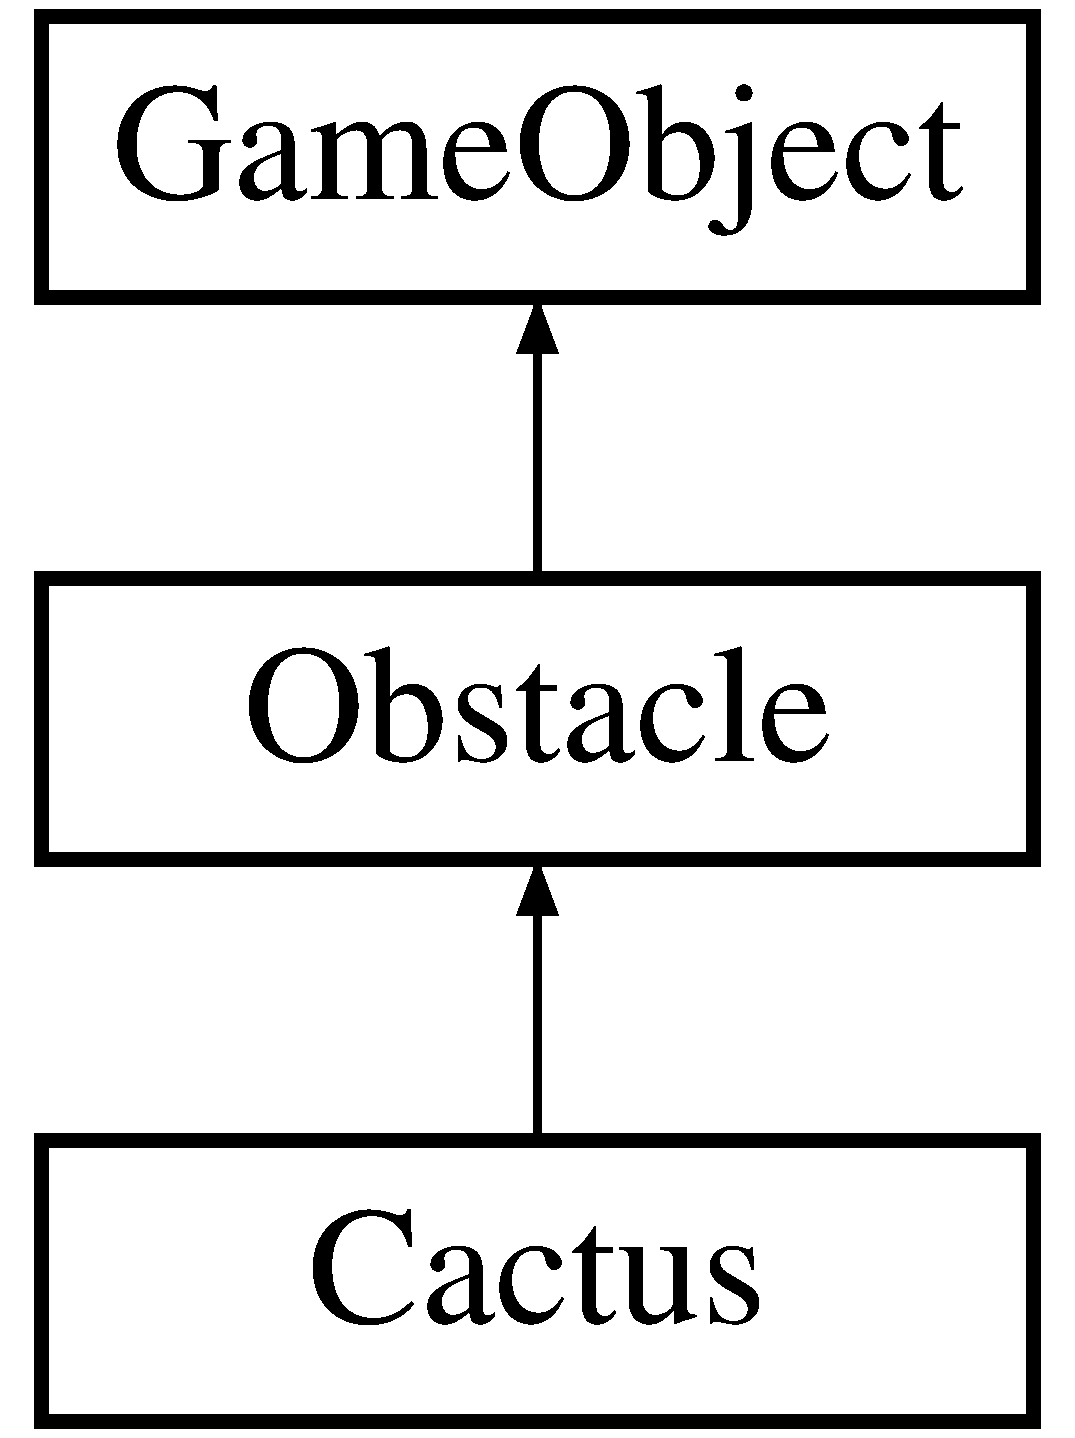
\includegraphics[height=3.000000cm]{class_cactus}
\end{center}
\end{figure}
\subsection*{Public Member Functions}
\begin{DoxyCompactItemize}
\item 
\mbox{\hyperlink{class_cactus_a1db8ad82bbfb944cf480d84b55ebd837}{Cactus}} (float distance, int type)
\begin{DoxyCompactList}\small\item\em Constructor. \end{DoxyCompactList}\item 
void \mbox{\hyperlink{class_cactus_aa432a0a002a0027ca294813d11cb76f3}{Update}} (float increment)
\begin{DoxyCompactList}\small\item\em Update method. \end{DoxyCompactList}\item 
\mbox{\Hypertarget{class_cactus_aad137061a9d2432ac47f4c28b23644c3}\label{class_cactus_aad137061a9d2432ac47f4c28b23644c3}} 
virtual \mbox{\hyperlink{class_cactus_aad137061a9d2432ac47f4c28b23644c3}{$\sim$\+Cactus}} ()
\begin{DoxyCompactList}\small\item\em Default destructor. \end{DoxyCompactList}\end{DoxyCompactItemize}
\subsection*{Additional Inherited Members}


\subsection{Detailed Description}
\mbox{\hyperlink{_cactus_8h_source}{Cactus.\+h}}. 

\mbox{\hyperlink{class_cactus}{Cactus}} subclass

Created\+: 20.\+08.\+2018. Author \+: Robert Gerstmajer 

\subsection{Constructor \& Destructor Documentation}
\mbox{\Hypertarget{class_cactus_a1db8ad82bbfb944cf480d84b55ebd837}\label{class_cactus_a1db8ad82bbfb944cf480d84b55ebd837}} 
\index{Cactus@{Cactus}!Cactus@{Cactus}}
\index{Cactus@{Cactus}!Cactus@{Cactus}}
\subsubsection{\texorpdfstring{Cactus()}{Cactus()}}
{\footnotesize\ttfamily Cactus\+::\+Cactus (\begin{DoxyParamCaption}\item[{float}]{distance,  }\item[{int}]{type }\end{DoxyParamCaption})}



Constructor. 

Cactus.\+cpp.

Creates a cactus at distance, with certain type 
\begin{DoxyParams}{Parameters}
{\em distance} & \\
\hline
{\em type} & Implementation of the \mbox{\hyperlink{class_cactus}{Cactus}} class\\
\hline
\end{DoxyParams}
Created\+: 20.\+08.\+2018. Author \+: Robert Gerstmajer 

\subsection{Member Function Documentation}
\mbox{\Hypertarget{class_cactus_aa432a0a002a0027ca294813d11cb76f3}\label{class_cactus_aa432a0a002a0027ca294813d11cb76f3}} 
\index{Cactus@{Cactus}!Update@{Update}}
\index{Update@{Update}!Cactus@{Cactus}}
\subsubsection{\texorpdfstring{Update()}{Update()}}
{\footnotesize\ttfamily void Cactus\+::\+Update (\begin{DoxyParamCaption}\item[{float}]{increment }\end{DoxyParamCaption})\hspace{0.3cm}{\ttfamily [virtual]}}



Update method. 

Moves sprite to the left according to increment 
\begin{DoxyParams}{Parameters}
{\em increment} & How much to move the sprite \\
\hline
\end{DoxyParams}


Implements \mbox{\hyperlink{class_obstacle_ad7bd00104a2c53cfb7421ca5986644af}{Obstacle}}.



The documentation for this class was generated from the following files\+:\begin{DoxyCompactItemize}
\item 
Cactus.\+h\item 
Cactus.\+cpp\end{DoxyCompactItemize}

\hypertarget{classtinyxml2_1_1_dyn_array}{}\section{tinyxml2\+:\+:Dyn\+Array$<$ T, I\+N\+I\+T\+I\+A\+L\+\_\+\+S\+I\+ZE $>$ Class Template Reference}
\label{classtinyxml2_1_1_dyn_array}\index{tinyxml2\+::\+Dyn\+Array$<$ T, I\+N\+I\+T\+I\+A\+L\+\_\+\+S\+I\+Z\+E $>$@{tinyxml2\+::\+Dyn\+Array$<$ T, I\+N\+I\+T\+I\+A\+L\+\_\+\+S\+I\+Z\+E $>$}}


{\ttfamily \#include $<$tinyxml2.\+h$>$}

\subsection*{Public Member Functions}
\begin{DoxyCompactItemize}
\item 
\mbox{\hyperlink{classtinyxml2_1_1_dyn_array_aaad72f384e761c70a4519183eb8fea17}{Dyn\+Array}} ()
\item 
\mbox{\hyperlink{classtinyxml2_1_1_dyn_array_a4a6aefdca7fe0d3f4068e31870a5adee}{$\sim$\+Dyn\+Array}} ()
\item 
void \mbox{\hyperlink{classtinyxml2_1_1_dyn_array_af87a804cd831226d069274b44b74b8bc}{Clear}} ()
\item 
void \mbox{\hyperlink{classtinyxml2_1_1_dyn_array_aea7ffe983b5d3284bd43171afd7c99d0}{Push}} (T t)
\item 
T $\ast$ \mbox{\hyperlink{classtinyxml2_1_1_dyn_array_ad289abee8cd02b26e215f1b63d2043f1}{Push\+Arr}} (int count)
\item 
T \mbox{\hyperlink{classtinyxml2_1_1_dyn_array_a27a3f2f6f869815b6eabb3ea40cf0712}{Pop}} ()
\item 
void \mbox{\hyperlink{classtinyxml2_1_1_dyn_array_ab8b8c94a2312ab27e2846f0d61ef677a}{Pop\+Arr}} (int count)
\item 
bool \mbox{\hyperlink{classtinyxml2_1_1_dyn_array_a044fc26f44ed3e96ffaeac542188149e}{Empty}} () const
\item 
T \& \mbox{\hyperlink{classtinyxml2_1_1_dyn_array_a756cf4e7464c711aa720e2b17a251daa}{operator\mbox{[}$\,$\mbox{]}}} (int i)
\item 
const T \& \mbox{\hyperlink{classtinyxml2_1_1_dyn_array_a474a5cd9bc97ea32b3dcef4c773125e1}{operator\mbox{[}$\,$\mbox{]}}} (int i) const
\item 
const T \& \mbox{\hyperlink{classtinyxml2_1_1_dyn_array_a5e4e1e408e646688503dec77c77c9d59}{Peek\+Top}} () const
\item 
int \mbox{\hyperlink{classtinyxml2_1_1_dyn_array_a67614d80847eb92cab330f1a5849a9a2}{Size}} () const
\item 
int \mbox{\hyperlink{classtinyxml2_1_1_dyn_array_a8e101fdf5b4248ac119d7dca6d0f5421}{Capacity}} () const
\item 
void \mbox{\hyperlink{classtinyxml2_1_1_dyn_array_aa72c644f8b5e9ec5dab5b66c88f5665f}{Swap\+Remove}} (int i)
\item 
const T $\ast$ \mbox{\hyperlink{classtinyxml2_1_1_dyn_array_a60b33e61cf10b3fd900ee46692dc0fe9}{Mem}} () const
\item 
T $\ast$ \mbox{\hyperlink{classtinyxml2_1_1_dyn_array_a2f0842cd666e2ad951f1a8bd6561fa40}{Mem}} ()
\end{DoxyCompactItemize}


\subsection{Constructor \& Destructor Documentation}
\mbox{\Hypertarget{classtinyxml2_1_1_dyn_array_aaad72f384e761c70a4519183eb8fea17}\label{classtinyxml2_1_1_dyn_array_aaad72f384e761c70a4519183eb8fea17}} 
\index{tinyxml2\+::\+Dyn\+Array@{tinyxml2\+::\+Dyn\+Array}!Dyn\+Array@{Dyn\+Array}}
\index{Dyn\+Array@{Dyn\+Array}!tinyxml2\+::\+Dyn\+Array@{tinyxml2\+::\+Dyn\+Array}}
\subsubsection{\texorpdfstring{Dyn\+Array()}{DynArray()}}
{\footnotesize\ttfamily template$<$class T, int I\+N\+I\+T\+I\+A\+L\+\_\+\+S\+I\+ZE$>$ \\
\mbox{\hyperlink{classtinyxml2_1_1_dyn_array}{tinyxml2\+::\+Dyn\+Array}}$<$ T, I\+N\+I\+T\+I\+A\+L\+\_\+\+S\+I\+ZE $>$\+::\mbox{\hyperlink{classtinyxml2_1_1_dyn_array}{Dyn\+Array}} (\begin{DoxyParamCaption}{ }\end{DoxyParamCaption})\hspace{0.3cm}{\ttfamily [inline]}}

\mbox{\Hypertarget{classtinyxml2_1_1_dyn_array_a4a6aefdca7fe0d3f4068e31870a5adee}\label{classtinyxml2_1_1_dyn_array_a4a6aefdca7fe0d3f4068e31870a5adee}} 
\index{tinyxml2\+::\+Dyn\+Array@{tinyxml2\+::\+Dyn\+Array}!````~Dyn\+Array@{$\sim$\+Dyn\+Array}}
\index{````~Dyn\+Array@{$\sim$\+Dyn\+Array}!tinyxml2\+::\+Dyn\+Array@{tinyxml2\+::\+Dyn\+Array}}
\subsubsection{\texorpdfstring{$\sim$\+Dyn\+Array()}{~DynArray()}}
{\footnotesize\ttfamily template$<$class T, int I\+N\+I\+T\+I\+A\+L\+\_\+\+S\+I\+ZE$>$ \\
\mbox{\hyperlink{classtinyxml2_1_1_dyn_array}{tinyxml2\+::\+Dyn\+Array}}$<$ T, I\+N\+I\+T\+I\+A\+L\+\_\+\+S\+I\+ZE $>$\+::$\sim$\mbox{\hyperlink{classtinyxml2_1_1_dyn_array}{Dyn\+Array}} (\begin{DoxyParamCaption}{ }\end{DoxyParamCaption})\hspace{0.3cm}{\ttfamily [inline]}}



\subsection{Member Function Documentation}
\mbox{\Hypertarget{classtinyxml2_1_1_dyn_array_a8e101fdf5b4248ac119d7dca6d0f5421}\label{classtinyxml2_1_1_dyn_array_a8e101fdf5b4248ac119d7dca6d0f5421}} 
\index{tinyxml2\+::\+Dyn\+Array@{tinyxml2\+::\+Dyn\+Array}!Capacity@{Capacity}}
\index{Capacity@{Capacity}!tinyxml2\+::\+Dyn\+Array@{tinyxml2\+::\+Dyn\+Array}}
\subsubsection{\texorpdfstring{Capacity()}{Capacity()}}
{\footnotesize\ttfamily template$<$class T, int I\+N\+I\+T\+I\+A\+L\+\_\+\+S\+I\+ZE$>$ \\
int \mbox{\hyperlink{classtinyxml2_1_1_dyn_array}{tinyxml2\+::\+Dyn\+Array}}$<$ T, I\+N\+I\+T\+I\+A\+L\+\_\+\+S\+I\+ZE $>$\+::Capacity (\begin{DoxyParamCaption}{ }\end{DoxyParamCaption}) const\hspace{0.3cm}{\ttfamily [inline]}}

\mbox{\Hypertarget{classtinyxml2_1_1_dyn_array_af87a804cd831226d069274b44b74b8bc}\label{classtinyxml2_1_1_dyn_array_af87a804cd831226d069274b44b74b8bc}} 
\index{tinyxml2\+::\+Dyn\+Array@{tinyxml2\+::\+Dyn\+Array}!Clear@{Clear}}
\index{Clear@{Clear}!tinyxml2\+::\+Dyn\+Array@{tinyxml2\+::\+Dyn\+Array}}
\subsubsection{\texorpdfstring{Clear()}{Clear()}}
{\footnotesize\ttfamily template$<$class T, int I\+N\+I\+T\+I\+A\+L\+\_\+\+S\+I\+ZE$>$ \\
void \mbox{\hyperlink{classtinyxml2_1_1_dyn_array}{tinyxml2\+::\+Dyn\+Array}}$<$ T, I\+N\+I\+T\+I\+A\+L\+\_\+\+S\+I\+ZE $>$\+::Clear (\begin{DoxyParamCaption}{ }\end{DoxyParamCaption})\hspace{0.3cm}{\ttfamily [inline]}}

\mbox{\Hypertarget{classtinyxml2_1_1_dyn_array_a044fc26f44ed3e96ffaeac542188149e}\label{classtinyxml2_1_1_dyn_array_a044fc26f44ed3e96ffaeac542188149e}} 
\index{tinyxml2\+::\+Dyn\+Array@{tinyxml2\+::\+Dyn\+Array}!Empty@{Empty}}
\index{Empty@{Empty}!tinyxml2\+::\+Dyn\+Array@{tinyxml2\+::\+Dyn\+Array}}
\subsubsection{\texorpdfstring{Empty()}{Empty()}}
{\footnotesize\ttfamily template$<$class T, int I\+N\+I\+T\+I\+A\+L\+\_\+\+S\+I\+ZE$>$ \\
bool \mbox{\hyperlink{classtinyxml2_1_1_dyn_array}{tinyxml2\+::\+Dyn\+Array}}$<$ T, I\+N\+I\+T\+I\+A\+L\+\_\+\+S\+I\+ZE $>$\+::Empty (\begin{DoxyParamCaption}{ }\end{DoxyParamCaption}) const\hspace{0.3cm}{\ttfamily [inline]}}

\mbox{\Hypertarget{classtinyxml2_1_1_dyn_array_a60b33e61cf10b3fd900ee46692dc0fe9}\label{classtinyxml2_1_1_dyn_array_a60b33e61cf10b3fd900ee46692dc0fe9}} 
\index{tinyxml2\+::\+Dyn\+Array@{tinyxml2\+::\+Dyn\+Array}!Mem@{Mem}}
\index{Mem@{Mem}!tinyxml2\+::\+Dyn\+Array@{tinyxml2\+::\+Dyn\+Array}}
\subsubsection{\texorpdfstring{Mem()}{Mem()}\hspace{0.1cm}{\footnotesize\ttfamily [1/2]}}
{\footnotesize\ttfamily template$<$class T, int I\+N\+I\+T\+I\+A\+L\+\_\+\+S\+I\+ZE$>$ \\
const T$\ast$ \mbox{\hyperlink{classtinyxml2_1_1_dyn_array}{tinyxml2\+::\+Dyn\+Array}}$<$ T, I\+N\+I\+T\+I\+A\+L\+\_\+\+S\+I\+ZE $>$\+::Mem (\begin{DoxyParamCaption}{ }\end{DoxyParamCaption}) const\hspace{0.3cm}{\ttfamily [inline]}}

\mbox{\Hypertarget{classtinyxml2_1_1_dyn_array_a2f0842cd666e2ad951f1a8bd6561fa40}\label{classtinyxml2_1_1_dyn_array_a2f0842cd666e2ad951f1a8bd6561fa40}} 
\index{tinyxml2\+::\+Dyn\+Array@{tinyxml2\+::\+Dyn\+Array}!Mem@{Mem}}
\index{Mem@{Mem}!tinyxml2\+::\+Dyn\+Array@{tinyxml2\+::\+Dyn\+Array}}
\subsubsection{\texorpdfstring{Mem()}{Mem()}\hspace{0.1cm}{\footnotesize\ttfamily [2/2]}}
{\footnotesize\ttfamily template$<$class T, int I\+N\+I\+T\+I\+A\+L\+\_\+\+S\+I\+ZE$>$ \\
T$\ast$ \mbox{\hyperlink{classtinyxml2_1_1_dyn_array}{tinyxml2\+::\+Dyn\+Array}}$<$ T, I\+N\+I\+T\+I\+A\+L\+\_\+\+S\+I\+ZE $>$\+::Mem (\begin{DoxyParamCaption}{ }\end{DoxyParamCaption})\hspace{0.3cm}{\ttfamily [inline]}}

\mbox{\Hypertarget{classtinyxml2_1_1_dyn_array_a756cf4e7464c711aa720e2b17a251daa}\label{classtinyxml2_1_1_dyn_array_a756cf4e7464c711aa720e2b17a251daa}} 
\index{tinyxml2\+::\+Dyn\+Array@{tinyxml2\+::\+Dyn\+Array}!operator\mbox{[}\mbox{]}@{operator[]}}
\index{operator\mbox{[}\mbox{]}@{operator[]}!tinyxml2\+::\+Dyn\+Array@{tinyxml2\+::\+Dyn\+Array}}
\subsubsection{\texorpdfstring{operator[]()}{operator[]()}\hspace{0.1cm}{\footnotesize\ttfamily [1/2]}}
{\footnotesize\ttfamily template$<$class T, int I\+N\+I\+T\+I\+A\+L\+\_\+\+S\+I\+ZE$>$ \\
T\& \mbox{\hyperlink{classtinyxml2_1_1_dyn_array}{tinyxml2\+::\+Dyn\+Array}}$<$ T, I\+N\+I\+T\+I\+A\+L\+\_\+\+S\+I\+ZE $>$\+::operator\mbox{[}$\,$\mbox{]} (\begin{DoxyParamCaption}\item[{int}]{i }\end{DoxyParamCaption})\hspace{0.3cm}{\ttfamily [inline]}}

\mbox{\Hypertarget{classtinyxml2_1_1_dyn_array_a474a5cd9bc97ea32b3dcef4c773125e1}\label{classtinyxml2_1_1_dyn_array_a474a5cd9bc97ea32b3dcef4c773125e1}} 
\index{tinyxml2\+::\+Dyn\+Array@{tinyxml2\+::\+Dyn\+Array}!operator\mbox{[}\mbox{]}@{operator[]}}
\index{operator\mbox{[}\mbox{]}@{operator[]}!tinyxml2\+::\+Dyn\+Array@{tinyxml2\+::\+Dyn\+Array}}
\subsubsection{\texorpdfstring{operator[]()}{operator[]()}\hspace{0.1cm}{\footnotesize\ttfamily [2/2]}}
{\footnotesize\ttfamily template$<$class T, int I\+N\+I\+T\+I\+A\+L\+\_\+\+S\+I\+ZE$>$ \\
const T\& \mbox{\hyperlink{classtinyxml2_1_1_dyn_array}{tinyxml2\+::\+Dyn\+Array}}$<$ T, I\+N\+I\+T\+I\+A\+L\+\_\+\+S\+I\+ZE $>$\+::operator\mbox{[}$\,$\mbox{]} (\begin{DoxyParamCaption}\item[{int}]{i }\end{DoxyParamCaption}) const\hspace{0.3cm}{\ttfamily [inline]}}

\mbox{\Hypertarget{classtinyxml2_1_1_dyn_array_a5e4e1e408e646688503dec77c77c9d59}\label{classtinyxml2_1_1_dyn_array_a5e4e1e408e646688503dec77c77c9d59}} 
\index{tinyxml2\+::\+Dyn\+Array@{tinyxml2\+::\+Dyn\+Array}!Peek\+Top@{Peek\+Top}}
\index{Peek\+Top@{Peek\+Top}!tinyxml2\+::\+Dyn\+Array@{tinyxml2\+::\+Dyn\+Array}}
\subsubsection{\texorpdfstring{Peek\+Top()}{PeekTop()}}
{\footnotesize\ttfamily template$<$class T, int I\+N\+I\+T\+I\+A\+L\+\_\+\+S\+I\+ZE$>$ \\
const T\& \mbox{\hyperlink{classtinyxml2_1_1_dyn_array}{tinyxml2\+::\+Dyn\+Array}}$<$ T, I\+N\+I\+T\+I\+A\+L\+\_\+\+S\+I\+ZE $>$\+::Peek\+Top (\begin{DoxyParamCaption}{ }\end{DoxyParamCaption}) const\hspace{0.3cm}{\ttfamily [inline]}}

\mbox{\Hypertarget{classtinyxml2_1_1_dyn_array_a27a3f2f6f869815b6eabb3ea40cf0712}\label{classtinyxml2_1_1_dyn_array_a27a3f2f6f869815b6eabb3ea40cf0712}} 
\index{tinyxml2\+::\+Dyn\+Array@{tinyxml2\+::\+Dyn\+Array}!Pop@{Pop}}
\index{Pop@{Pop}!tinyxml2\+::\+Dyn\+Array@{tinyxml2\+::\+Dyn\+Array}}
\subsubsection{\texorpdfstring{Pop()}{Pop()}}
{\footnotesize\ttfamily template$<$class T, int I\+N\+I\+T\+I\+A\+L\+\_\+\+S\+I\+ZE$>$ \\
T \mbox{\hyperlink{classtinyxml2_1_1_dyn_array}{tinyxml2\+::\+Dyn\+Array}}$<$ T, I\+N\+I\+T\+I\+A\+L\+\_\+\+S\+I\+ZE $>$\+::Pop (\begin{DoxyParamCaption}{ }\end{DoxyParamCaption})\hspace{0.3cm}{\ttfamily [inline]}}

\mbox{\Hypertarget{classtinyxml2_1_1_dyn_array_ab8b8c94a2312ab27e2846f0d61ef677a}\label{classtinyxml2_1_1_dyn_array_ab8b8c94a2312ab27e2846f0d61ef677a}} 
\index{tinyxml2\+::\+Dyn\+Array@{tinyxml2\+::\+Dyn\+Array}!Pop\+Arr@{Pop\+Arr}}
\index{Pop\+Arr@{Pop\+Arr}!tinyxml2\+::\+Dyn\+Array@{tinyxml2\+::\+Dyn\+Array}}
\subsubsection{\texorpdfstring{Pop\+Arr()}{PopArr()}}
{\footnotesize\ttfamily template$<$class T, int I\+N\+I\+T\+I\+A\+L\+\_\+\+S\+I\+ZE$>$ \\
void \mbox{\hyperlink{classtinyxml2_1_1_dyn_array}{tinyxml2\+::\+Dyn\+Array}}$<$ T, I\+N\+I\+T\+I\+A\+L\+\_\+\+S\+I\+ZE $>$\+::Pop\+Arr (\begin{DoxyParamCaption}\item[{int}]{count }\end{DoxyParamCaption})\hspace{0.3cm}{\ttfamily [inline]}}

\mbox{\Hypertarget{classtinyxml2_1_1_dyn_array_aea7ffe983b5d3284bd43171afd7c99d0}\label{classtinyxml2_1_1_dyn_array_aea7ffe983b5d3284bd43171afd7c99d0}} 
\index{tinyxml2\+::\+Dyn\+Array@{tinyxml2\+::\+Dyn\+Array}!Push@{Push}}
\index{Push@{Push}!tinyxml2\+::\+Dyn\+Array@{tinyxml2\+::\+Dyn\+Array}}
\subsubsection{\texorpdfstring{Push()}{Push()}}
{\footnotesize\ttfamily template$<$class T, int I\+N\+I\+T\+I\+A\+L\+\_\+\+S\+I\+ZE$>$ \\
void \mbox{\hyperlink{classtinyxml2_1_1_dyn_array}{tinyxml2\+::\+Dyn\+Array}}$<$ T, I\+N\+I\+T\+I\+A\+L\+\_\+\+S\+I\+ZE $>$\+::Push (\begin{DoxyParamCaption}\item[{T}]{t }\end{DoxyParamCaption})\hspace{0.3cm}{\ttfamily [inline]}}

\mbox{\Hypertarget{classtinyxml2_1_1_dyn_array_ad289abee8cd02b26e215f1b63d2043f1}\label{classtinyxml2_1_1_dyn_array_ad289abee8cd02b26e215f1b63d2043f1}} 
\index{tinyxml2\+::\+Dyn\+Array@{tinyxml2\+::\+Dyn\+Array}!Push\+Arr@{Push\+Arr}}
\index{Push\+Arr@{Push\+Arr}!tinyxml2\+::\+Dyn\+Array@{tinyxml2\+::\+Dyn\+Array}}
\subsubsection{\texorpdfstring{Push\+Arr()}{PushArr()}}
{\footnotesize\ttfamily template$<$class T, int I\+N\+I\+T\+I\+A\+L\+\_\+\+S\+I\+ZE$>$ \\
T$\ast$ \mbox{\hyperlink{classtinyxml2_1_1_dyn_array}{tinyxml2\+::\+Dyn\+Array}}$<$ T, I\+N\+I\+T\+I\+A\+L\+\_\+\+S\+I\+ZE $>$\+::Push\+Arr (\begin{DoxyParamCaption}\item[{int}]{count }\end{DoxyParamCaption})\hspace{0.3cm}{\ttfamily [inline]}}

\mbox{\Hypertarget{classtinyxml2_1_1_dyn_array_a67614d80847eb92cab330f1a5849a9a2}\label{classtinyxml2_1_1_dyn_array_a67614d80847eb92cab330f1a5849a9a2}} 
\index{tinyxml2\+::\+Dyn\+Array@{tinyxml2\+::\+Dyn\+Array}!Size@{Size}}
\index{Size@{Size}!tinyxml2\+::\+Dyn\+Array@{tinyxml2\+::\+Dyn\+Array}}
\subsubsection{\texorpdfstring{Size()}{Size()}}
{\footnotesize\ttfamily template$<$class T, int I\+N\+I\+T\+I\+A\+L\+\_\+\+S\+I\+ZE$>$ \\
int \mbox{\hyperlink{classtinyxml2_1_1_dyn_array}{tinyxml2\+::\+Dyn\+Array}}$<$ T, I\+N\+I\+T\+I\+A\+L\+\_\+\+S\+I\+ZE $>$\+::Size (\begin{DoxyParamCaption}{ }\end{DoxyParamCaption}) const\hspace{0.3cm}{\ttfamily [inline]}}

\mbox{\Hypertarget{classtinyxml2_1_1_dyn_array_aa72c644f8b5e9ec5dab5b66c88f5665f}\label{classtinyxml2_1_1_dyn_array_aa72c644f8b5e9ec5dab5b66c88f5665f}} 
\index{tinyxml2\+::\+Dyn\+Array@{tinyxml2\+::\+Dyn\+Array}!Swap\+Remove@{Swap\+Remove}}
\index{Swap\+Remove@{Swap\+Remove}!tinyxml2\+::\+Dyn\+Array@{tinyxml2\+::\+Dyn\+Array}}
\subsubsection{\texorpdfstring{Swap\+Remove()}{SwapRemove()}}
{\footnotesize\ttfamily template$<$class T, int I\+N\+I\+T\+I\+A\+L\+\_\+\+S\+I\+ZE$>$ \\
void \mbox{\hyperlink{classtinyxml2_1_1_dyn_array}{tinyxml2\+::\+Dyn\+Array}}$<$ T, I\+N\+I\+T\+I\+A\+L\+\_\+\+S\+I\+ZE $>$\+::Swap\+Remove (\begin{DoxyParamCaption}\item[{int}]{i }\end{DoxyParamCaption})\hspace{0.3cm}{\ttfamily [inline]}}



The documentation for this class was generated from the following file\+:\begin{DoxyCompactItemize}
\item 
\mbox{\hyperlink{tinyxml2_8h}{tinyxml2.\+h}}\end{DoxyCompactItemize}

\hypertarget{structtinyxml2_1_1_entity}{}\section{tinyxml2\+:\+:Entity Struct Reference}
\label{structtinyxml2_1_1_entity}\index{tinyxml2\+::\+Entity@{tinyxml2\+::\+Entity}}
\subsection*{Public Attributes}
\begin{DoxyCompactItemize}
\item 
const char $\ast$ \mbox{\hyperlink{structtinyxml2_1_1_entity_ab330f5d665d29bfc811ecfa76315894b}{pattern}}
\item 
int \mbox{\hyperlink{structtinyxml2_1_1_entity_a25e2b57cb59cb4fa68f283d7cb570f21}{length}}
\item 
char \mbox{\hyperlink{structtinyxml2_1_1_entity_a7334e81e33b4615655a403711b24f3ed}{value}}
\end{DoxyCompactItemize}


\subsection{Member Data Documentation}
\mbox{\Hypertarget{structtinyxml2_1_1_entity_a25e2b57cb59cb4fa68f283d7cb570f21}\label{structtinyxml2_1_1_entity_a25e2b57cb59cb4fa68f283d7cb570f21}} 
\index{tinyxml2\+::\+Entity@{tinyxml2\+::\+Entity}!length@{length}}
\index{length@{length}!tinyxml2\+::\+Entity@{tinyxml2\+::\+Entity}}
\subsubsection{\texorpdfstring{length}{length}}
{\footnotesize\ttfamily int tinyxml2\+::\+Entity\+::length}

\mbox{\Hypertarget{structtinyxml2_1_1_entity_ab330f5d665d29bfc811ecfa76315894b}\label{structtinyxml2_1_1_entity_ab330f5d665d29bfc811ecfa76315894b}} 
\index{tinyxml2\+::\+Entity@{tinyxml2\+::\+Entity}!pattern@{pattern}}
\index{pattern@{pattern}!tinyxml2\+::\+Entity@{tinyxml2\+::\+Entity}}
\subsubsection{\texorpdfstring{pattern}{pattern}}
{\footnotesize\ttfamily const char$\ast$ tinyxml2\+::\+Entity\+::pattern}

\mbox{\Hypertarget{structtinyxml2_1_1_entity_a7334e81e33b4615655a403711b24f3ed}\label{structtinyxml2_1_1_entity_a7334e81e33b4615655a403711b24f3ed}} 
\index{tinyxml2\+::\+Entity@{tinyxml2\+::\+Entity}!value@{value}}
\index{value@{value}!tinyxml2\+::\+Entity@{tinyxml2\+::\+Entity}}
\subsubsection{\texorpdfstring{value}{value}}
{\footnotesize\ttfamily char tinyxml2\+::\+Entity\+::value}



The documentation for this struct was generated from the following file\+:\begin{DoxyCompactItemize}
\item 
\mbox{\hyperlink{tinyxml2_8cpp}{tinyxml2.\+cpp}}\end{DoxyCompactItemize}

\hypertarget{class_game_object}{}\section{Game\+Object Class Reference}
\label{class_game_object}\index{Game\+Object@{Game\+Object}}


\mbox{\hyperlink{_game_object_8h_source}{Game\+Object.\+h}}.  




{\ttfamily \#include $<$Game\+Object.\+h$>$}

Inheritance diagram for Game\+Object\+:\begin{figure}[H]
\begin{center}
\leavevmode
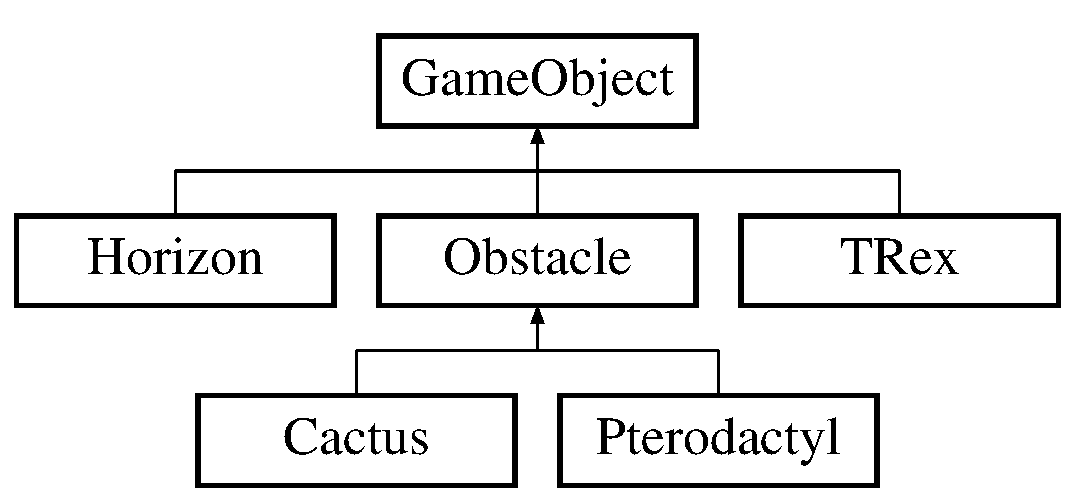
\includegraphics[height=3.000000cm]{class_game_object}
\end{center}
\end{figure}
\subsection*{Public Member Functions}
\begin{DoxyCompactItemize}
\item 
\mbox{\hyperlink{class_game_object_a0348e3ee2e83d56eafca7a3547f432c4}{Game\+Object}} ()
\begin{DoxyCompactList}\small\item\em Default constructor. \end{DoxyCompactList}\item 
void \mbox{\hyperlink{class_game_object_a7ba982dd7315ab822c18dd9892112316}{Draw}} (sf\+::\+Render\+Window $\ast$window)
\begin{DoxyCompactList}\small\item\em Drawing method. \end{DoxyCompactList}\item 
bool \mbox{\hyperlink{class_game_object_a9f63ba7fa09d165f175858276f71d44b}{Colliding}} (\mbox{\hyperlink{class_game_object}{Game\+Object}} $\ast$obstacle)
\begin{DoxyCompactList}\small\item\em Collision checking method. \end{DoxyCompactList}\item 
float \mbox{\hyperlink{class_game_object_a274bf74e1658d845a0603be2972a63c4}{Get\+PositionX}} ()
\item 
float \mbox{\hyperlink{class_game_object_abe7e418773edb98562033fcfdf191dd9}{Get\+PositionY}} ()
\item 
\mbox{\Hypertarget{class_game_object_ab82dfdb656f9051c0587e6593b2dda97}\label{class_game_object_ab82dfdb656f9051c0587e6593b2dda97}} 
\mbox{\hyperlink{class_game_object_ab82dfdb656f9051c0587e6593b2dda97}{$\sim$\+Game\+Object}} ()
\begin{DoxyCompactList}\small\item\em Default destructor. \end{DoxyCompactList}\end{DoxyCompactItemize}
\subsection*{Protected Member Functions}
\begin{DoxyCompactItemize}
\item 
sf\+::\+Sprite $\ast$ \mbox{\hyperlink{class_game_object_ab570c73233f2e8eb9fb3c043b1a68c4c}{Load\+Shape}} (sf\+::\+Texture $\ast$texture, const int height, const int width, const unsigned char $\ast$shape, bool is\+Bump=false)
\begin{DoxyCompactList}\small\item\em Shape loading method. \end{DoxyCompactList}\end{DoxyCompactItemize}
\subsection*{Protected Attributes}
\begin{DoxyCompactItemize}
\item 
\mbox{\Hypertarget{class_game_object_ac965ec6e2eba11bb1be2ecba57508329}\label{class_game_object_ac965ec6e2eba11bb1be2ecba57508329}} 
sf\+::\+Sprite $\ast$ {\bfseries sprite}
\item 
\mbox{\Hypertarget{class_game_object_a8cadf697830d86c59f4a193ad70b17b2}\label{class_game_object_a8cadf697830d86c59f4a193ad70b17b2}} 
sf\+::\+Float\+Rect {\bfseries shrunk\+Bounds}
\end{DoxyCompactItemize}


\subsection{Detailed Description}
\mbox{\hyperlink{_game_object_8h_source}{Game\+Object.\+h}}. 

\mbox{\hyperlink{class_game_object}{Game\+Object}} base class header file

Created\+: 20.\+08.\+2018. Author \+: Robert Gerstmajer 

\subsection{Constructor \& Destructor Documentation}
\mbox{\Hypertarget{class_game_object_a0348e3ee2e83d56eafca7a3547f432c4}\label{class_game_object_a0348e3ee2e83d56eafca7a3547f432c4}} 
\index{Game\+Object@{Game\+Object}!Game\+Object@{Game\+Object}}
\index{Game\+Object@{Game\+Object}!Game\+Object@{Game\+Object}}
\subsubsection{\texorpdfstring{Game\+Object()}{GameObject()}}
{\footnotesize\ttfamily Game\+Object\+::\+Game\+Object (\begin{DoxyParamCaption}{ }\end{DoxyParamCaption})}



Default constructor. 

Game\+Object.\+cpp.

Implementation of the \mbox{\hyperlink{class_game_object}{Game\+Object}} class

Created\+: 20.\+08.\+2018. Author \+: Robert Gerstmajer 

\subsection{Member Function Documentation}
\mbox{\Hypertarget{class_game_object_a9f63ba7fa09d165f175858276f71d44b}\label{class_game_object_a9f63ba7fa09d165f175858276f71d44b}} 
\index{Game\+Object@{Game\+Object}!Colliding@{Colliding}}
\index{Colliding@{Colliding}!Game\+Object@{Game\+Object}}
\subsubsection{\texorpdfstring{Colliding()}{Colliding()}}
{\footnotesize\ttfamily bool Game\+Object\+::\+Colliding (\begin{DoxyParamCaption}\item[{\mbox{\hyperlink{class_game_object}{Game\+Object}} $\ast$}]{obstacle }\end{DoxyParamCaption})}



Collision checking method. 

Checks if the \mbox{\hyperlink{class_game_object}{Game\+Object}} sprite is colliding with obstacle 
\begin{DoxyParams}{Parameters}
{\em obstacle} & to check collision with \\
\hline
\end{DoxyParams}
\mbox{\Hypertarget{class_game_object_a7ba982dd7315ab822c18dd9892112316}\label{class_game_object_a7ba982dd7315ab822c18dd9892112316}} 
\index{Game\+Object@{Game\+Object}!Draw@{Draw}}
\index{Draw@{Draw}!Game\+Object@{Game\+Object}}
\subsubsection{\texorpdfstring{Draw()}{Draw()}}
{\footnotesize\ttfamily void Game\+Object\+::\+Draw (\begin{DoxyParamCaption}\item[{sf\+::\+Render\+Window $\ast$}]{window }\end{DoxyParamCaption})}



Drawing method. 

Draws sprite on sfml Render\+Window 
\begin{DoxyParams}{Parameters}
{\em window} & sfml Render\+Window to draw on \\
\hline
\end{DoxyParams}
\mbox{\Hypertarget{class_game_object_a274bf74e1658d845a0603be2972a63c4}\label{class_game_object_a274bf74e1658d845a0603be2972a63c4}} 
\index{Game\+Object@{Game\+Object}!Get\+PositionX@{Get\+PositionX}}
\index{Get\+PositionX@{Get\+PositionX}!Game\+Object@{Game\+Object}}
\subsubsection{\texorpdfstring{Get\+Position\+X()}{GetPositionX()}}
{\footnotesize\ttfamily float Game\+Object\+::\+Get\+PositionX (\begin{DoxyParamCaption}{ }\end{DoxyParamCaption})\hspace{0.3cm}{\ttfamily [inline]}}

Returns the sprite location on X axis \mbox{\Hypertarget{class_game_object_abe7e418773edb98562033fcfdf191dd9}\label{class_game_object_abe7e418773edb98562033fcfdf191dd9}} 
\index{Game\+Object@{Game\+Object}!Get\+PositionY@{Get\+PositionY}}
\index{Get\+PositionY@{Get\+PositionY}!Game\+Object@{Game\+Object}}
\subsubsection{\texorpdfstring{Get\+Position\+Y()}{GetPositionY()}}
{\footnotesize\ttfamily float Game\+Object\+::\+Get\+PositionY (\begin{DoxyParamCaption}{ }\end{DoxyParamCaption})\hspace{0.3cm}{\ttfamily [inline]}}

Returns the sprite location on Y axis \mbox{\Hypertarget{class_game_object_ab570c73233f2e8eb9fb3c043b1a68c4c}\label{class_game_object_ab570c73233f2e8eb9fb3c043b1a68c4c}} 
\index{Game\+Object@{Game\+Object}!Load\+Shape@{Load\+Shape}}
\index{Load\+Shape@{Load\+Shape}!Game\+Object@{Game\+Object}}
\subsubsection{\texorpdfstring{Load\+Shape()}{LoadShape()}}
{\footnotesize\ttfamily sf\+::\+Sprite $\ast$ Game\+Object\+::\+Load\+Shape (\begin{DoxyParamCaption}\item[{sf\+::\+Texture $\ast$}]{texture,  }\item[{const int}]{height,  }\item[{const int}]{width,  }\item[{const unsigned char $\ast$}]{shape,  }\item[{bool}]{is\+Bump = {\ttfamily false} }\end{DoxyParamCaption})\hspace{0.3cm}{\ttfamily [protected]}}



Shape loading method. 

Loads shape into sprite 
\begin{DoxyParams}{Parameters}
{\em texture} & sfml Texture buffer for creating the sprite \\
\hline
{\em height} & sprite height \\
\hline
{\em width} & sprite width \\
\hline
{\em shape} & sprite\+Shape taken from \mbox{\hyperlink{_globals_8h_source}{Globals.\+h}} \\
\hline
{\em is\+Bump} & if the shape is a horizon bump, background is black, otherwise transparent \\
\hline
\end{DoxyParams}


The documentation for this class was generated from the following files\+:\begin{DoxyCompactItemize}
\item 
Game\+Object.\+h\item 
Game\+Object.\+cpp\end{DoxyCompactItemize}

\hypertarget{class_horizon}{}\section{Horizon Class Reference}
\label{class_horizon}\index{Horizon@{Horizon}}


\mbox{\hyperlink{_horizon_8h}{Horizon.\+h}}.  




{\ttfamily \#include $<$Horizon.\+h$>$}

Inheritance diagram for Horizon\+:\begin{figure}[H]
\begin{center}
\leavevmode
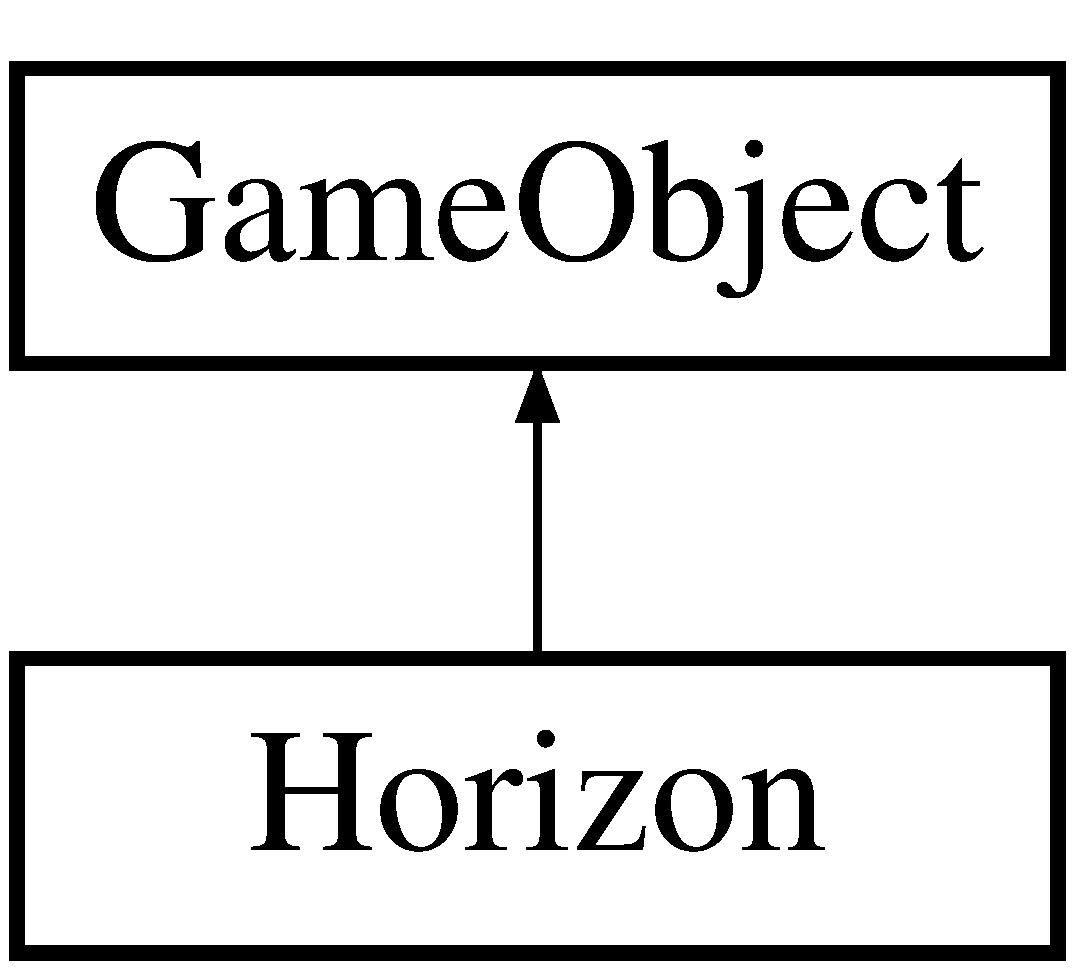
\includegraphics[height=2.000000cm]{class_horizon}
\end{center}
\end{figure}
\subsection*{Public Member Functions}
\begin{DoxyCompactItemize}
\item 
\mbox{\hyperlink{class_horizon_adbdceabfe68477247ecb2c469e4d8187}{Horizon}} (int type)
\begin{DoxyCompactList}\small\item\em Constructor. \end{DoxyCompactList}\item 
\mbox{\hyperlink{class_game_object_ad5092169e581fb0772e01026882ea0c8}{game\+Object\+Type}} \mbox{\hyperlink{class_horizon_abe319d6ba70ce79028ba9175a4bcd4e6}{Get\+Game\+Object\+Type}} ()
\item 
void \mbox{\hyperlink{class_horizon_a845596ecfc2953f0d124e5fd0d7cb1d3}{Move}} (float increment)
\begin{DoxyCompactList}\small\item\em Move method. \end{DoxyCompactList}\item 
void \mbox{\hyperlink{class_horizon_a80800c898ea4cd015ae865351a6aec4c}{Init}} ()
\item 
\mbox{\hyperlink{class_horizon_a4b917eb3365308d9ab6e1ab5c8891299}{$\sim$\+Horizon}} ()
\begin{DoxyCompactList}\small\item\em Default destructor. \end{DoxyCompactList}\end{DoxyCompactItemize}
\subsection*{Additional Inherited Members}


\subsection{Detailed Description}
\mbox{\hyperlink{_horizon_8h}{Horizon.\+h}}. 

\mbox{\hyperlink{class_horizon}{Horizon}} subclass for horizon bumps

Created\+: 20.\+08.\+2018. Author \+: Robert Gerstmajer 

\subsection{Constructor \& Destructor Documentation}
\mbox{\Hypertarget{class_horizon_adbdceabfe68477247ecb2c469e4d8187}\label{class_horizon_adbdceabfe68477247ecb2c469e4d8187}} 
\index{Horizon@{Horizon}!Horizon@{Horizon}}
\index{Horizon@{Horizon}!Horizon@{Horizon}}
\subsubsection{\texorpdfstring{Horizon()}{Horizon()}}
{\footnotesize\ttfamily Horizon\+::\+Horizon (\begin{DoxyParamCaption}\item[{int}]{type }\end{DoxyParamCaption})}



Constructor. 

\mbox{\hyperlink{_horizon_8cpp}{Horizon.\+cpp}}.

\mbox{\hyperlink{class_horizon}{Horizon}} bump constructr 
\begin{DoxyParams}{Parameters}
{\em type} & Type of bump (1 or 2)\\
\hline
\end{DoxyParams}
Implementation of the \mbox{\hyperlink{class_horizon}{Horizon}} class

Created\+: 20.\+08.\+2018. Author \+: Robert Gerstmajer \mbox{\Hypertarget{class_horizon_a4b917eb3365308d9ab6e1ab5c8891299}\label{class_horizon_a4b917eb3365308d9ab6e1ab5c8891299}} 
\index{Horizon@{Horizon}!````~Horizon@{$\sim$\+Horizon}}
\index{````~Horizon@{$\sim$\+Horizon}!Horizon@{Horizon}}
\subsubsection{\texorpdfstring{$\sim$\+Horizon()}{~Horizon()}}
{\footnotesize\ttfamily Horizon\+::$\sim$\+Horizon (\begin{DoxyParamCaption}{ }\end{DoxyParamCaption})}



Default destructor. 



\subsection{Member Function Documentation}
\mbox{\Hypertarget{class_horizon_abe319d6ba70ce79028ba9175a4bcd4e6}\label{class_horizon_abe319d6ba70ce79028ba9175a4bcd4e6}} 
\index{Horizon@{Horizon}!Get\+Game\+Object\+Type@{Get\+Game\+Object\+Type}}
\index{Get\+Game\+Object\+Type@{Get\+Game\+Object\+Type}!Horizon@{Horizon}}
\subsubsection{\texorpdfstring{Get\+Game\+Object\+Type()}{GetGameObjectType()}}
{\footnotesize\ttfamily \mbox{\hyperlink{class_game_object_ad5092169e581fb0772e01026882ea0c8}{game\+Object\+Type}} Horizon\+::\+Get\+Game\+Object\+Type (\begin{DoxyParamCaption}{ }\end{DoxyParamCaption})\hspace{0.3cm}{\ttfamily [inline]}}

\mbox{\Hypertarget{class_horizon_a80800c898ea4cd015ae865351a6aec4c}\label{class_horizon_a80800c898ea4cd015ae865351a6aec4c}} 
\index{Horizon@{Horizon}!Init@{Init}}
\index{Init@{Init}!Horizon@{Horizon}}
\subsubsection{\texorpdfstring{Init()}{Init()}}
{\footnotesize\ttfamily void Horizon\+::\+Init (\begin{DoxyParamCaption}{ }\end{DoxyParamCaption})\hspace{0.3cm}{\ttfamily [virtual]}}



Implements \mbox{\hyperlink{class_game_object_ab3b70fcc4e640ba2081508b1efb35536}{Game\+Object}}.

\mbox{\Hypertarget{class_horizon_a845596ecfc2953f0d124e5fd0d7cb1d3}\label{class_horizon_a845596ecfc2953f0d124e5fd0d7cb1d3}} 
\index{Horizon@{Horizon}!Move@{Move}}
\index{Move@{Move}!Horizon@{Horizon}}
\subsubsection{\texorpdfstring{Move()}{Move()}}
{\footnotesize\ttfamily void Horizon\+::\+Move (\begin{DoxyParamCaption}\item[{float}]{increment }\end{DoxyParamCaption})}



Move method. 

Moves sprite to the left according to increment 
\begin{DoxyParams}{Parameters}
{\em increment} & How much to move the sprite \\
\hline
\end{DoxyParams}


The documentation for this class was generated from the following files\+:\begin{DoxyCompactItemize}
\item 
\mbox{\hyperlink{_horizon_8h}{Horizon.\+h}}\item 
\mbox{\hyperlink{_horizon_8cpp}{Horizon.\+cpp}}\end{DoxyCompactItemize}

\hypertarget{structtinyxml2_1_1_long_fits_into_size_t_minus_one}{}\section{tinyxml2\+:\+:Long\+Fits\+Into\+Size\+T\+Minus\+One$<$ bool $>$ Struct Template Reference}
\label{structtinyxml2_1_1_long_fits_into_size_t_minus_one}\index{tinyxml2\+::\+Long\+Fits\+Into\+Size\+T\+Minus\+One$<$ bool $>$@{tinyxml2\+::\+Long\+Fits\+Into\+Size\+T\+Minus\+One$<$ bool $>$}}
\subsection*{Static Public Member Functions}
\begin{DoxyCompactItemize}
\item 
\mbox{\Hypertarget{structtinyxml2_1_1_long_fits_into_size_t_minus_one_a3057710104ab733963eb32fda0bc374c}\label{structtinyxml2_1_1_long_fits_into_size_t_minus_one_a3057710104ab733963eb32fda0bc374c}} 
static bool {\bfseries Fits} (unsigned long value)
\end{DoxyCompactItemize}


The documentation for this struct was generated from the following file\+:\begin{DoxyCompactItemize}
\item 
tinyxml2.\+cpp\end{DoxyCompactItemize}

\hypertarget{structtinyxml2_1_1_long_fits_into_size_t_minus_one_3_01false_01_4}{}\section{tinyxml2\+:\+:Long\+Fits\+Into\+Size\+T\+Minus\+One$<$ false $>$ Struct Template Reference}
\label{structtinyxml2_1_1_long_fits_into_size_t_minus_one_3_01false_01_4}\index{tinyxml2\+::\+Long\+Fits\+Into\+Size\+T\+Minus\+One$<$ false $>$@{tinyxml2\+::\+Long\+Fits\+Into\+Size\+T\+Minus\+One$<$ false $>$}}
\subsection*{Static Public Member Functions}
\begin{DoxyCompactItemize}
\item 
\mbox{\Hypertarget{structtinyxml2_1_1_long_fits_into_size_t_minus_one_3_01false_01_4_a29b01087f38a951276df69d358dc0764}\label{structtinyxml2_1_1_long_fits_into_size_t_minus_one_3_01false_01_4_a29b01087f38a951276df69d358dc0764}} 
static bool {\bfseries Fits} (unsigned long)
\end{DoxyCompactItemize}


The documentation for this struct was generated from the following file\+:\begin{DoxyCompactItemize}
\item 
tinyxml2.\+cpp\end{DoxyCompactItemize}

\hypertarget{classtinyxml2_1_1_mem_pool}{}\section{tinyxml2\+:\+:Mem\+Pool Class Reference}
\label{classtinyxml2_1_1_mem_pool}\index{tinyxml2\+::\+Mem\+Pool@{tinyxml2\+::\+Mem\+Pool}}


{\ttfamily \#include $<$tinyxml2.\+h$>$}

Inheritance diagram for tinyxml2\+:\+:Mem\+Pool\+:\begin{figure}[H]
\begin{center}
\leavevmode
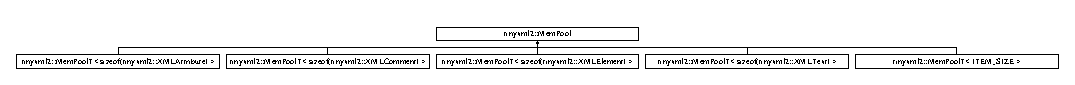
\includegraphics[height=0.691358cm]{classtinyxml2_1_1_mem_pool}
\end{center}
\end{figure}
\subsection*{Public Member Functions}
\begin{DoxyCompactItemize}
\item 
\mbox{\hyperlink{classtinyxml2_1_1_mem_pool_a9101a0083d7370c85bd5aaaba7157f84}{Mem\+Pool}} ()
\item 
virtual \mbox{\hyperlink{classtinyxml2_1_1_mem_pool_ae55ad9e3faeca702e6ccbb38fdbcad72}{$\sim$\+Mem\+Pool}} ()
\item 
virtual int \mbox{\hyperlink{classtinyxml2_1_1_mem_pool_a0c518d49e3a94bde566f61e13b7240bb}{Item\+Size}} () const =0
\item 
virtual void $\ast$ \mbox{\hyperlink{classtinyxml2_1_1_mem_pool_a4f977b5fed752c0bbfe5295f469d6449}{Alloc}} ()=0
\item 
virtual void \mbox{\hyperlink{classtinyxml2_1_1_mem_pool_a49e3bfac2cba2ebd6776b31e571f64f7}{Free}} (void $\ast$)=0
\item 
virtual void \mbox{\hyperlink{classtinyxml2_1_1_mem_pool_ac5804dd1387b2e4de5eef710076a0db1}{Set\+Tracked}} ()=0
\end{DoxyCompactItemize}


\subsection{Constructor \& Destructor Documentation}
\mbox{\Hypertarget{classtinyxml2_1_1_mem_pool_a9101a0083d7370c85bd5aaaba7157f84}\label{classtinyxml2_1_1_mem_pool_a9101a0083d7370c85bd5aaaba7157f84}} 
\index{tinyxml2\+::\+Mem\+Pool@{tinyxml2\+::\+Mem\+Pool}!Mem\+Pool@{Mem\+Pool}}
\index{Mem\+Pool@{Mem\+Pool}!tinyxml2\+::\+Mem\+Pool@{tinyxml2\+::\+Mem\+Pool}}
\subsubsection{\texorpdfstring{Mem\+Pool()}{MemPool()}}
{\footnotesize\ttfamily tinyxml2\+::\+Mem\+Pool\+::\+Mem\+Pool (\begin{DoxyParamCaption}{ }\end{DoxyParamCaption})\hspace{0.3cm}{\ttfamily [inline]}}

\mbox{\Hypertarget{classtinyxml2_1_1_mem_pool_ae55ad9e3faeca702e6ccbb38fdbcad72}\label{classtinyxml2_1_1_mem_pool_ae55ad9e3faeca702e6ccbb38fdbcad72}} 
\index{tinyxml2\+::\+Mem\+Pool@{tinyxml2\+::\+Mem\+Pool}!````~Mem\+Pool@{$\sim$\+Mem\+Pool}}
\index{````~Mem\+Pool@{$\sim$\+Mem\+Pool}!tinyxml2\+::\+Mem\+Pool@{tinyxml2\+::\+Mem\+Pool}}
\subsubsection{\texorpdfstring{$\sim$\+Mem\+Pool()}{~MemPool()}}
{\footnotesize\ttfamily virtual tinyxml2\+::\+Mem\+Pool\+::$\sim$\+Mem\+Pool (\begin{DoxyParamCaption}{ }\end{DoxyParamCaption})\hspace{0.3cm}{\ttfamily [inline]}, {\ttfamily [virtual]}}



\subsection{Member Function Documentation}
\mbox{\Hypertarget{classtinyxml2_1_1_mem_pool_a4f977b5fed752c0bbfe5295f469d6449}\label{classtinyxml2_1_1_mem_pool_a4f977b5fed752c0bbfe5295f469d6449}} 
\index{tinyxml2\+::\+Mem\+Pool@{tinyxml2\+::\+Mem\+Pool}!Alloc@{Alloc}}
\index{Alloc@{Alloc}!tinyxml2\+::\+Mem\+Pool@{tinyxml2\+::\+Mem\+Pool}}
\subsubsection{\texorpdfstring{Alloc()}{Alloc()}}
{\footnotesize\ttfamily virtual void$\ast$ tinyxml2\+::\+Mem\+Pool\+::\+Alloc (\begin{DoxyParamCaption}{ }\end{DoxyParamCaption})\hspace{0.3cm}{\ttfamily [pure virtual]}}



Implemented in \mbox{\hyperlink{classtinyxml2_1_1_mem_pool_t_a810fd2b0caf56b8b688e55f2768f96c7}{tinyxml2\+::\+Mem\+Pool\+T$<$ I\+T\+E\+M\+\_\+\+S\+I\+Z\+E $>$}}, \mbox{\hyperlink{classtinyxml2_1_1_mem_pool_t_a810fd2b0caf56b8b688e55f2768f96c7}{tinyxml2\+::\+Mem\+Pool\+T$<$ sizeof(tinyxml2\+::\+X\+M\+L\+Comment) $>$}}, \mbox{\hyperlink{classtinyxml2_1_1_mem_pool_t_a810fd2b0caf56b8b688e55f2768f96c7}{tinyxml2\+::\+Mem\+Pool\+T$<$ sizeof(tinyxml2\+::\+X\+M\+L\+Text) $>$}}, \mbox{\hyperlink{classtinyxml2_1_1_mem_pool_t_a810fd2b0caf56b8b688e55f2768f96c7}{tinyxml2\+::\+Mem\+Pool\+T$<$ sizeof(tinyxml2\+::\+X\+M\+L\+Attribute) $>$}}, and \mbox{\hyperlink{classtinyxml2_1_1_mem_pool_t_a810fd2b0caf56b8b688e55f2768f96c7}{tinyxml2\+::\+Mem\+Pool\+T$<$ sizeof(tinyxml2\+::\+X\+M\+L\+Element) $>$}}.

\mbox{\Hypertarget{classtinyxml2_1_1_mem_pool_a49e3bfac2cba2ebd6776b31e571f64f7}\label{classtinyxml2_1_1_mem_pool_a49e3bfac2cba2ebd6776b31e571f64f7}} 
\index{tinyxml2\+::\+Mem\+Pool@{tinyxml2\+::\+Mem\+Pool}!Free@{Free}}
\index{Free@{Free}!tinyxml2\+::\+Mem\+Pool@{tinyxml2\+::\+Mem\+Pool}}
\subsubsection{\texorpdfstring{Free()}{Free()}}
{\footnotesize\ttfamily virtual void tinyxml2\+::\+Mem\+Pool\+::\+Free (\begin{DoxyParamCaption}\item[{void $\ast$}]{ }\end{DoxyParamCaption})\hspace{0.3cm}{\ttfamily [pure virtual]}}



Implemented in \mbox{\hyperlink{classtinyxml2_1_1_mem_pool_t_a408ce0918e9d3d5e5e1cc4896944875f}{tinyxml2\+::\+Mem\+Pool\+T$<$ I\+T\+E\+M\+\_\+\+S\+I\+Z\+E $>$}}, \mbox{\hyperlink{classtinyxml2_1_1_mem_pool_t_a408ce0918e9d3d5e5e1cc4896944875f}{tinyxml2\+::\+Mem\+Pool\+T$<$ sizeof(tinyxml2\+::\+X\+M\+L\+Comment) $>$}}, \mbox{\hyperlink{classtinyxml2_1_1_mem_pool_t_a408ce0918e9d3d5e5e1cc4896944875f}{tinyxml2\+::\+Mem\+Pool\+T$<$ sizeof(tinyxml2\+::\+X\+M\+L\+Text) $>$}}, \mbox{\hyperlink{classtinyxml2_1_1_mem_pool_t_a408ce0918e9d3d5e5e1cc4896944875f}{tinyxml2\+::\+Mem\+Pool\+T$<$ sizeof(tinyxml2\+::\+X\+M\+L\+Attribute) $>$}}, and \mbox{\hyperlink{classtinyxml2_1_1_mem_pool_t_a408ce0918e9d3d5e5e1cc4896944875f}{tinyxml2\+::\+Mem\+Pool\+T$<$ sizeof(tinyxml2\+::\+X\+M\+L\+Element) $>$}}.

\mbox{\Hypertarget{classtinyxml2_1_1_mem_pool_a0c518d49e3a94bde566f61e13b7240bb}\label{classtinyxml2_1_1_mem_pool_a0c518d49e3a94bde566f61e13b7240bb}} 
\index{tinyxml2\+::\+Mem\+Pool@{tinyxml2\+::\+Mem\+Pool}!Item\+Size@{Item\+Size}}
\index{Item\+Size@{Item\+Size}!tinyxml2\+::\+Mem\+Pool@{tinyxml2\+::\+Mem\+Pool}}
\subsubsection{\texorpdfstring{Item\+Size()}{ItemSize()}}
{\footnotesize\ttfamily virtual int tinyxml2\+::\+Mem\+Pool\+::\+Item\+Size (\begin{DoxyParamCaption}{ }\end{DoxyParamCaption}) const\hspace{0.3cm}{\ttfamily [pure virtual]}}



Implemented in \mbox{\hyperlink{classtinyxml2_1_1_mem_pool_t_a54e4d9b343459ef1731314a99877ff35}{tinyxml2\+::\+Mem\+Pool\+T$<$ I\+T\+E\+M\+\_\+\+S\+I\+Z\+E $>$}}, \mbox{\hyperlink{classtinyxml2_1_1_mem_pool_t_a54e4d9b343459ef1731314a99877ff35}{tinyxml2\+::\+Mem\+Pool\+T$<$ sizeof(tinyxml2\+::\+X\+M\+L\+Comment) $>$}}, \mbox{\hyperlink{classtinyxml2_1_1_mem_pool_t_a54e4d9b343459ef1731314a99877ff35}{tinyxml2\+::\+Mem\+Pool\+T$<$ sizeof(tinyxml2\+::\+X\+M\+L\+Text) $>$}}, \mbox{\hyperlink{classtinyxml2_1_1_mem_pool_t_a54e4d9b343459ef1731314a99877ff35}{tinyxml2\+::\+Mem\+Pool\+T$<$ sizeof(tinyxml2\+::\+X\+M\+L\+Attribute) $>$}}, and \mbox{\hyperlink{classtinyxml2_1_1_mem_pool_t_a54e4d9b343459ef1731314a99877ff35}{tinyxml2\+::\+Mem\+Pool\+T$<$ sizeof(tinyxml2\+::\+X\+M\+L\+Element) $>$}}.

\mbox{\Hypertarget{classtinyxml2_1_1_mem_pool_ac5804dd1387b2e4de5eef710076a0db1}\label{classtinyxml2_1_1_mem_pool_ac5804dd1387b2e4de5eef710076a0db1}} 
\index{tinyxml2\+::\+Mem\+Pool@{tinyxml2\+::\+Mem\+Pool}!Set\+Tracked@{Set\+Tracked}}
\index{Set\+Tracked@{Set\+Tracked}!tinyxml2\+::\+Mem\+Pool@{tinyxml2\+::\+Mem\+Pool}}
\subsubsection{\texorpdfstring{Set\+Tracked()}{SetTracked()}}
{\footnotesize\ttfamily virtual void tinyxml2\+::\+Mem\+Pool\+::\+Set\+Tracked (\begin{DoxyParamCaption}{ }\end{DoxyParamCaption})\hspace{0.3cm}{\ttfamily [pure virtual]}}



Implemented in \mbox{\hyperlink{classtinyxml2_1_1_mem_pool_t_aee3c611215ae08cce41a940bf2763027}{tinyxml2\+::\+Mem\+Pool\+T$<$ I\+T\+E\+M\+\_\+\+S\+I\+Z\+E $>$}}, \mbox{\hyperlink{classtinyxml2_1_1_mem_pool_t_aee3c611215ae08cce41a940bf2763027}{tinyxml2\+::\+Mem\+Pool\+T$<$ sizeof(tinyxml2\+::\+X\+M\+L\+Comment) $>$}}, \mbox{\hyperlink{classtinyxml2_1_1_mem_pool_t_aee3c611215ae08cce41a940bf2763027}{tinyxml2\+::\+Mem\+Pool\+T$<$ sizeof(tinyxml2\+::\+X\+M\+L\+Text) $>$}}, \mbox{\hyperlink{classtinyxml2_1_1_mem_pool_t_aee3c611215ae08cce41a940bf2763027}{tinyxml2\+::\+Mem\+Pool\+T$<$ sizeof(tinyxml2\+::\+X\+M\+L\+Attribute) $>$}}, and \mbox{\hyperlink{classtinyxml2_1_1_mem_pool_t_aee3c611215ae08cce41a940bf2763027}{tinyxml2\+::\+Mem\+Pool\+T$<$ sizeof(tinyxml2\+::\+X\+M\+L\+Element) $>$}}.



The documentation for this class was generated from the following file\+:\begin{DoxyCompactItemize}
\item 
\mbox{\hyperlink{tinyxml2_8h}{tinyxml2.\+h}}\end{DoxyCompactItemize}

\hypertarget{classtinyxml2_1_1_mem_pool_t}{}\section{tinyxml2\+:\+:Mem\+PoolT$<$ I\+T\+E\+M\+\_\+\+S\+I\+ZE $>$ Class Template Reference}
\label{classtinyxml2_1_1_mem_pool_t}\index{tinyxml2\+::\+Mem\+Pool\+T$<$ I\+T\+E\+M\+\_\+\+S\+I\+Z\+E $>$@{tinyxml2\+::\+Mem\+Pool\+T$<$ I\+T\+E\+M\+\_\+\+S\+I\+Z\+E $>$}}
Inheritance diagram for tinyxml2\+:\+:Mem\+PoolT$<$ I\+T\+E\+M\+\_\+\+S\+I\+ZE $>$\+:\begin{figure}[H]
\begin{center}
\leavevmode
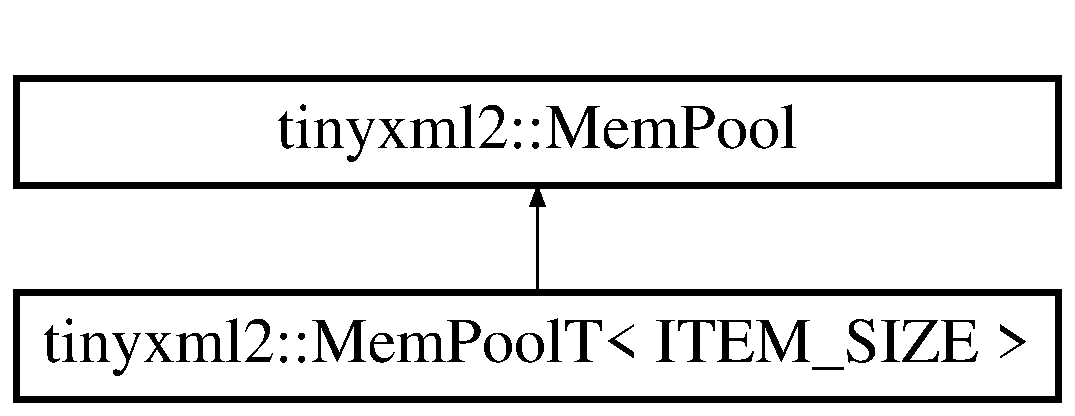
\includegraphics[height=2.000000cm]{classtinyxml2_1_1_mem_pool_t}
\end{center}
\end{figure}
\subsection*{Public Types}
\begin{DoxyCompactItemize}
\item 
\mbox{\Hypertarget{classtinyxml2_1_1_mem_pool_t_a04cf45156e6f913f93972869ff8a1d94}\label{classtinyxml2_1_1_mem_pool_t_a04cf45156e6f913f93972869ff8a1d94}} 
enum \{ {\bfseries I\+T\+E\+M\+S\+\_\+\+P\+E\+R\+\_\+\+B\+L\+O\+CK} = (4 $\ast$ 1024) / I\+T\+E\+M\+\_\+\+S\+I\+ZE
 \}
\end{DoxyCompactItemize}
\subsection*{Public Member Functions}
\begin{DoxyCompactItemize}
\item 
\mbox{\Hypertarget{classtinyxml2_1_1_mem_pool_t_a22d595caa0e9d23aa080f49ca6475fdd}\label{classtinyxml2_1_1_mem_pool_t_a22d595caa0e9d23aa080f49ca6475fdd}} 
void {\bfseries Clear} ()
\item 
\mbox{\Hypertarget{classtinyxml2_1_1_mem_pool_t_a54e4d9b343459ef1731314a99877ff35}\label{classtinyxml2_1_1_mem_pool_t_a54e4d9b343459ef1731314a99877ff35}} 
virtual int {\bfseries Item\+Size} () const
\item 
\mbox{\Hypertarget{classtinyxml2_1_1_mem_pool_t_a445a6c80151ba6268b24ec62a7c84d74}\label{classtinyxml2_1_1_mem_pool_t_a445a6c80151ba6268b24ec62a7c84d74}} 
int {\bfseries Current\+Allocs} () const
\item 
\mbox{\Hypertarget{classtinyxml2_1_1_mem_pool_t_a810fd2b0caf56b8b688e55f2768f96c7}\label{classtinyxml2_1_1_mem_pool_t_a810fd2b0caf56b8b688e55f2768f96c7}} 
virtual void $\ast$ {\bfseries Alloc} ()
\item 
\mbox{\Hypertarget{classtinyxml2_1_1_mem_pool_t_a408ce0918e9d3d5e5e1cc4896944875f}\label{classtinyxml2_1_1_mem_pool_t_a408ce0918e9d3d5e5e1cc4896944875f}} 
virtual void {\bfseries Free} (void $\ast$mem)
\item 
\mbox{\Hypertarget{classtinyxml2_1_1_mem_pool_t_a47eefbd934ef70d973ea41d41ab5f239}\label{classtinyxml2_1_1_mem_pool_t_a47eefbd934ef70d973ea41d41ab5f239}} 
void {\bfseries Trace} (const char $\ast$name)
\item 
\mbox{\Hypertarget{classtinyxml2_1_1_mem_pool_t_aee3c611215ae08cce41a940bf2763027}\label{classtinyxml2_1_1_mem_pool_t_aee3c611215ae08cce41a940bf2763027}} 
void {\bfseries Set\+Tracked} ()
\item 
\mbox{\Hypertarget{classtinyxml2_1_1_mem_pool_t_a3bcdc302ae15d2810e11192321a8f5f1}\label{classtinyxml2_1_1_mem_pool_t_a3bcdc302ae15d2810e11192321a8f5f1}} 
int {\bfseries Untracked} () const
\end{DoxyCompactItemize}


The documentation for this class was generated from the following file\+:\begin{DoxyCompactItemize}
\item 
tinyxml2.\+h\end{DoxyCompactItemize}

\hypertarget{class_obstacle}{}\section{Obstacle Class Reference}
\label{class_obstacle}\index{Obstacle@{Obstacle}}


\mbox{\hyperlink{_obstacle_8h_source}{Obstacle.\+h}}.  




{\ttfamily \#include $<$Obstacle.\+h$>$}

Inheritance diagram for Obstacle\+:\begin{figure}[H]
\begin{center}
\leavevmode
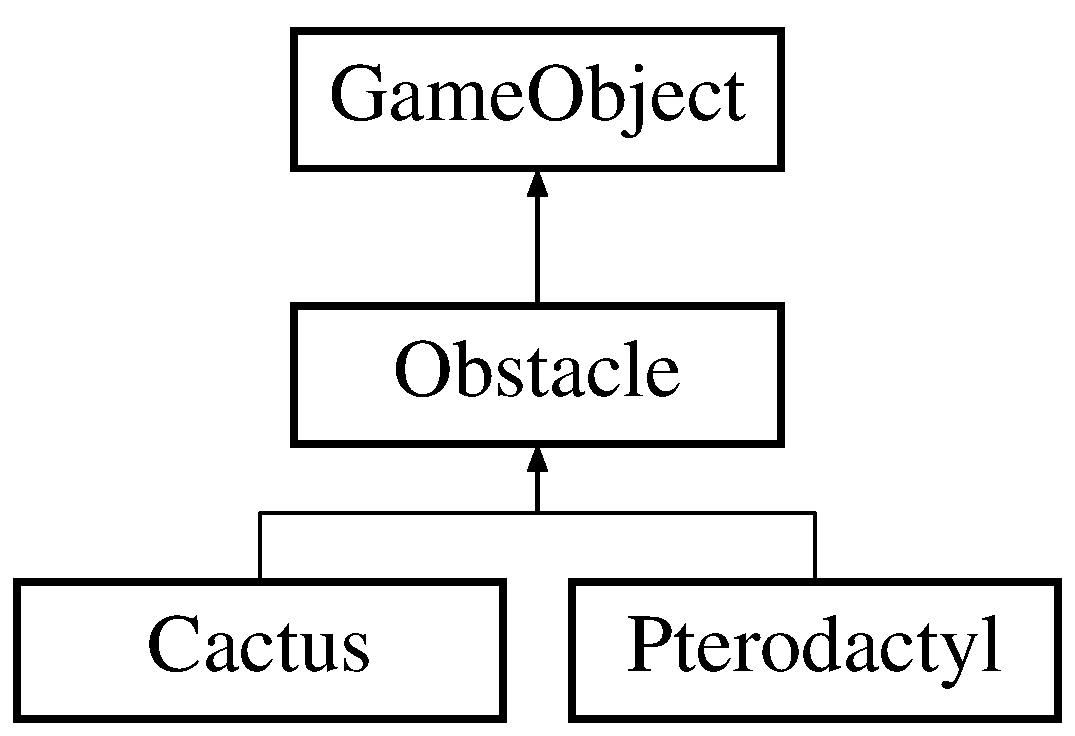
\includegraphics[height=3.000000cm]{class_obstacle}
\end{center}
\end{figure}
\subsection*{Public Member Functions}
\begin{DoxyCompactItemize}
\item 
\mbox{\hyperlink{class_obstacle_a8f734072321fa06a7b7dae2d5f50f352}{Obstacle}} ()
\begin{DoxyCompactList}\small\item\em Default constructor. \end{DoxyCompactList}\item 
void \mbox{\hyperlink{class_obstacle_af06377faeba537b4ff98ee2cfa061831}{Move}} (float increment)
\begin{DoxyCompactList}\small\item\em Move method. \end{DoxyCompactList}\item 
\mbox{\Hypertarget{class_obstacle_af2f9cc9c6cff75dca0974fd5ac4f71a9}\label{class_obstacle_af2f9cc9c6cff75dca0974fd5ac4f71a9}} 
\mbox{\hyperlink{class_obstacle_af2f9cc9c6cff75dca0974fd5ac4f71a9}{$\sim$\+Obstacle}} ()
\begin{DoxyCompactList}\small\item\em Default destructor. \end{DoxyCompactList}\end{DoxyCompactItemize}
\subsection*{Additional Inherited Members}


\subsection{Detailed Description}
\mbox{\hyperlink{_obstacle_8h_source}{Obstacle.\+h}}. 

\mbox{\hyperlink{class_obstacle}{Obstacle}} subclass for pterodactyls and cacti

Created\+: 20.\+08.\+2018. Author \+: Robert Gerstmajer 

\subsection{Constructor \& Destructor Documentation}
\mbox{\Hypertarget{class_obstacle_a8f734072321fa06a7b7dae2d5f50f352}\label{class_obstacle_a8f734072321fa06a7b7dae2d5f50f352}} 
\index{Obstacle@{Obstacle}!Obstacle@{Obstacle}}
\index{Obstacle@{Obstacle}!Obstacle@{Obstacle}}
\subsubsection{\texorpdfstring{Obstacle()}{Obstacle()}}
{\footnotesize\ttfamily Obstacle\+::\+Obstacle (\begin{DoxyParamCaption}{ }\end{DoxyParamCaption})}



Default constructor. 

Obstacle.\+cpp.

Implementation of the \mbox{\hyperlink{class_obstacle}{Obstacle}} class

Created\+: 20.\+08.\+2018. Author \+: Robert Gerstmajer 

\subsection{Member Function Documentation}
\mbox{\Hypertarget{class_obstacle_af06377faeba537b4ff98ee2cfa061831}\label{class_obstacle_af06377faeba537b4ff98ee2cfa061831}} 
\index{Obstacle@{Obstacle}!Move@{Move}}
\index{Move@{Move}!Obstacle@{Obstacle}}
\subsubsection{\texorpdfstring{Move()}{Move()}}
{\footnotesize\ttfamily void Obstacle\+::\+Move (\begin{DoxyParamCaption}\item[{float}]{increment }\end{DoxyParamCaption})}



Move method. 

Moves sprite to the left according to increment 
\begin{DoxyParams}{Parameters}
{\em increment} & How much to move the sprite \\
\hline
\end{DoxyParams}


The documentation for this class was generated from the following files\+:\begin{DoxyCompactItemize}
\item 
Obstacle.\+h\item 
Obstacle.\+cpp\end{DoxyCompactItemize}

\hypertarget{class_pterodactyl}{}\section{Pterodactyl Class Reference}
\label{class_pterodactyl}\index{Pterodactyl@{Pterodactyl}}


\mbox{\hyperlink{_pterodactyl_8h_source}{Pterodactyl.\+h}}.  




{\ttfamily \#include $<$Pterodactyl.\+h$>$}

Inheritance diagram for Pterodactyl\+:\begin{figure}[H]
\begin{center}
\leavevmode
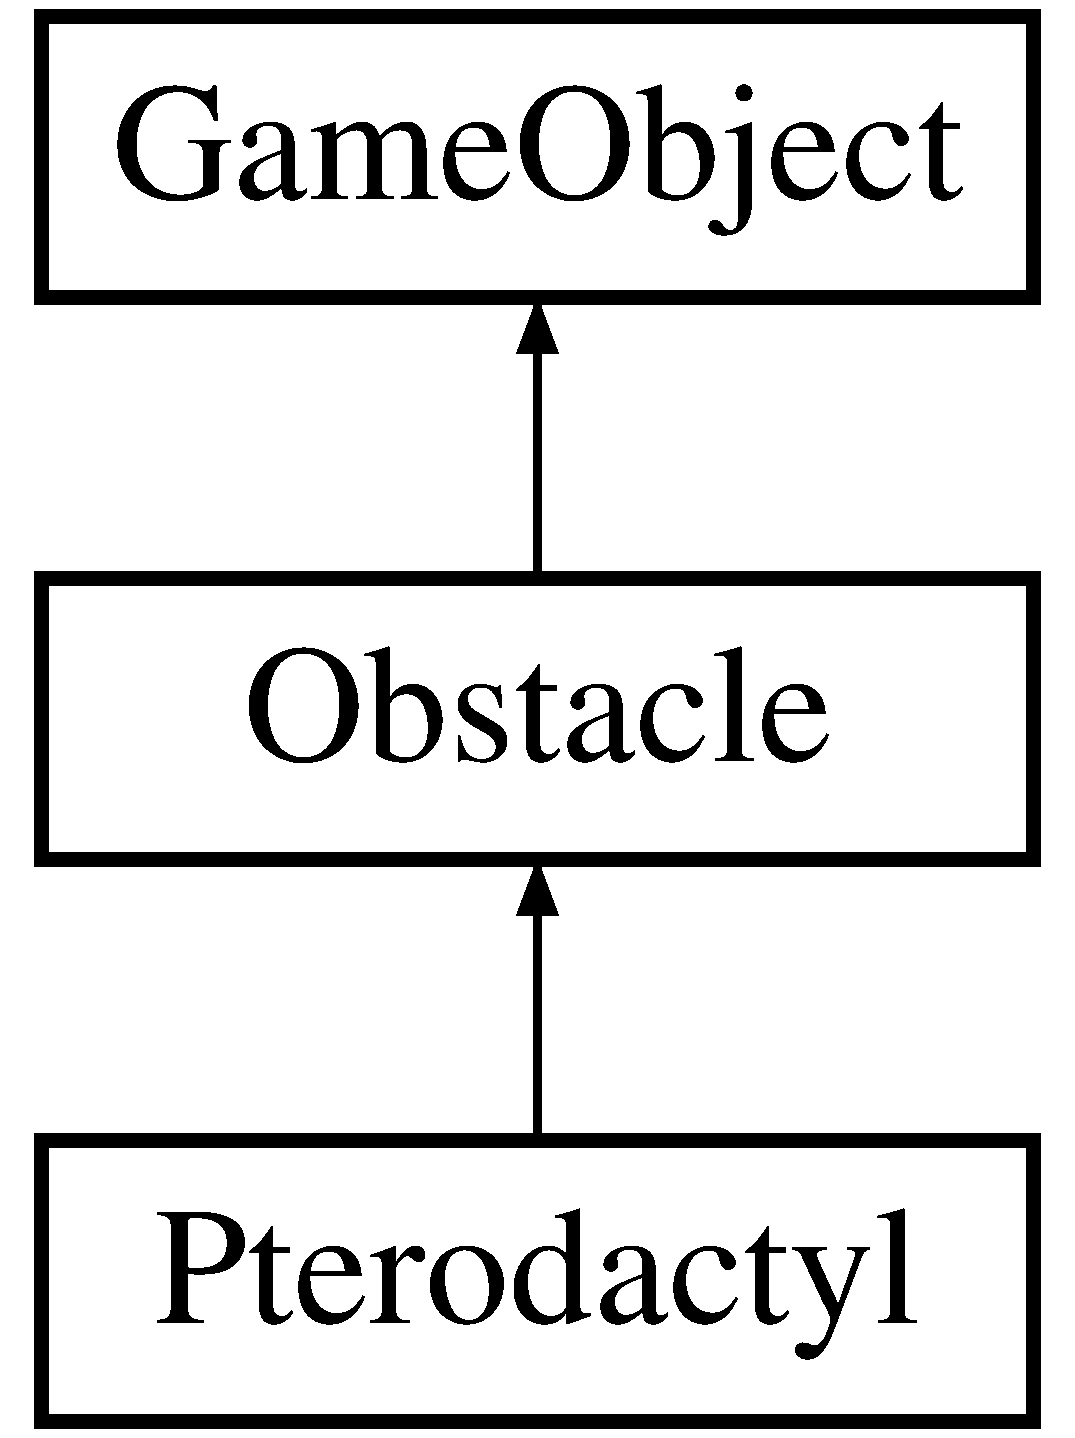
\includegraphics[height=3.000000cm]{class_pterodactyl}
\end{center}
\end{figure}
\subsection*{Public Member Functions}
\begin{DoxyCompactItemize}
\item 
\mbox{\hyperlink{class_pterodactyl_ae667ed30c8198eae8027bf34b2f90034}{Pterodactyl}} ()
\begin{DoxyCompactList}\small\item\em Default constructor. \end{DoxyCompactList}\item 
void \mbox{\hyperlink{class_pterodactyl_a55037eb1d5ed42027e9c0cf9891b3f70}{Init}} (int distance)
\begin{DoxyCompactList}\small\item\em Initialization method. \end{DoxyCompactList}\item 
\mbox{\Hypertarget{class_pterodactyl_a8ab71be091355092560c40746bf53bef}\label{class_pterodactyl_a8ab71be091355092560c40746bf53bef}} 
void \mbox{\hyperlink{class_pterodactyl_a8ab71be091355092560c40746bf53bef}{Update}} ()
\begin{DoxyCompactList}\small\item\em Update method. \end{DoxyCompactList}\item 
\mbox{\Hypertarget{class_pterodactyl_a57c101dcc34661693bb424770d590c0a}\label{class_pterodactyl_a57c101dcc34661693bb424770d590c0a}} 
\mbox{\hyperlink{class_pterodactyl_a57c101dcc34661693bb424770d590c0a}{$\sim$\+Pterodactyl}} ()
\begin{DoxyCompactList}\small\item\em Default destructor. \end{DoxyCompactList}\end{DoxyCompactItemize}
\subsection*{Additional Inherited Members}


\subsection{Detailed Description}
\mbox{\hyperlink{_pterodactyl_8h_source}{Pterodactyl.\+h}}. 

\mbox{\hyperlink{class_pterodactyl}{Pterodactyl}} subclass

Created\+: 20.\+08.\+2018. Author \+: Robert Gerstmajer 

\subsection{Constructor \& Destructor Documentation}
\mbox{\Hypertarget{class_pterodactyl_ae667ed30c8198eae8027bf34b2f90034}\label{class_pterodactyl_ae667ed30c8198eae8027bf34b2f90034}} 
\index{Pterodactyl@{Pterodactyl}!Pterodactyl@{Pterodactyl}}
\index{Pterodactyl@{Pterodactyl}!Pterodactyl@{Pterodactyl}}
\subsubsection{\texorpdfstring{Pterodactyl()}{Pterodactyl()}}
{\footnotesize\ttfamily Pterodactyl\+::\+Pterodactyl (\begin{DoxyParamCaption}{ }\end{DoxyParamCaption})}



Default constructor. 

Pterodactyl.\+cpp.

Implementation of the \mbox{\hyperlink{class_pterodactyl}{Pterodactyl}} class

Created\+: 20.\+08.\+2018. Author \+: Robert Gerstmajer 

\subsection{Member Function Documentation}
\mbox{\Hypertarget{class_pterodactyl_a55037eb1d5ed42027e9c0cf9891b3f70}\label{class_pterodactyl_a55037eb1d5ed42027e9c0cf9891b3f70}} 
\index{Pterodactyl@{Pterodactyl}!Init@{Init}}
\index{Init@{Init}!Pterodactyl@{Pterodactyl}}
\subsubsection{\texorpdfstring{Init()}{Init()}}
{\footnotesize\ttfamily void Pterodactyl\+::\+Init (\begin{DoxyParamCaption}\item[{int}]{distance }\end{DoxyParamCaption})}



Initialization method. 

Initializes random pterodactyl sprite on random distance.


\begin{DoxyParams}{Parameters}
{\em distance} & Distance of the pterodactyl being initialized \\
\hline
\end{DoxyParams}


The documentation for this class was generated from the following files\+:\begin{DoxyCompactItemize}
\item 
Pterodactyl.\+h\item 
Pterodactyl.\+cpp\end{DoxyCompactItemize}

\hypertarget{classtinyxml2_1_1_str_pair}{}\section{tinyxml2\+:\+:Str\+Pair Class Reference}
\label{classtinyxml2_1_1_str_pair}\index{tinyxml2\+::\+Str\+Pair@{tinyxml2\+::\+Str\+Pair}}


{\ttfamily \#include $<$tinyxml2.\+h$>$}

\subsection*{Public Types}
\begin{DoxyCompactItemize}
\item 
enum \{ \newline
\mbox{\hyperlink{classtinyxml2_1_1_str_pair_a0301ef962e15dd94574431f1c61266c5a4f1e01a55f8efe4ca72c32d454060237}{N\+E\+E\+D\+S\+\_\+\+E\+N\+T\+I\+T\+Y\+\_\+\+P\+R\+O\+C\+E\+S\+S\+I\+NG}} = 0x01, 
\mbox{\hyperlink{classtinyxml2_1_1_str_pair_a0301ef962e15dd94574431f1c61266c5a8f2045d56e70745d718672c0da91d0e0}{N\+E\+E\+D\+S\+\_\+\+N\+E\+W\+L\+I\+N\+E\+\_\+\+N\+O\+R\+M\+A\+L\+I\+Z\+A\+T\+I\+ON}} = 0x02, 
\mbox{\hyperlink{classtinyxml2_1_1_str_pair_a0301ef962e15dd94574431f1c61266c5a13996e9d4ed18fd2d6af59bbab291b63}{N\+E\+E\+D\+S\+\_\+\+W\+H\+I\+T\+E\+S\+P\+A\+C\+E\+\_\+\+C\+O\+L\+L\+A\+P\+S\+I\+NG}} = 0x04, 
\mbox{\hyperlink{classtinyxml2_1_1_str_pair_a0301ef962e15dd94574431f1c61266c5aae519eb5a639858591763aa5fc6cc953}{T\+E\+X\+T\+\_\+\+E\+L\+E\+M\+E\+NT}} = N\+E\+E\+D\+S\+\_\+\+E\+N\+T\+I\+T\+Y\+\_\+\+P\+R\+O\+C\+E\+S\+S\+I\+NG $\vert$ N\+E\+E\+D\+S\+\_\+\+N\+E\+W\+L\+I\+N\+E\+\_\+\+N\+O\+R\+M\+A\+L\+I\+Z\+A\+T\+I\+ON, 
\newline
\mbox{\hyperlink{classtinyxml2_1_1_str_pair_a0301ef962e15dd94574431f1c61266c5a96be48cf899bfeea0aa227f984f1fa63}{T\+E\+X\+T\+\_\+\+E\+L\+E\+M\+E\+N\+T\+\_\+\+L\+E\+A\+V\+E\+\_\+\+E\+N\+T\+I\+T\+I\+ES}} = N\+E\+E\+D\+S\+\_\+\+N\+E\+W\+L\+I\+N\+E\+\_\+\+N\+O\+R\+M\+A\+L\+I\+Z\+A\+T\+I\+ON, 
\mbox{\hyperlink{classtinyxml2_1_1_str_pair_a0301ef962e15dd94574431f1c61266c5aaab1cbefaa977e6f772b4e2575417aeb}{A\+T\+T\+R\+I\+B\+U\+T\+E\+\_\+\+N\+A\+ME}} = 0, 
\mbox{\hyperlink{classtinyxml2_1_1_str_pair_a0301ef962e15dd94574431f1c61266c5a6d72f9ce15f50e8bcd680edf66235dfd}{A\+T\+T\+R\+I\+B\+U\+T\+E\+\_\+\+V\+A\+L\+UE}} = N\+E\+E\+D\+S\+\_\+\+E\+N\+T\+I\+T\+Y\+\_\+\+P\+R\+O\+C\+E\+S\+S\+I\+NG $\vert$ N\+E\+E\+D\+S\+\_\+\+N\+E\+W\+L\+I\+N\+E\+\_\+\+N\+O\+R\+M\+A\+L\+I\+Z\+A\+T\+I\+ON, 
\mbox{\hyperlink{classtinyxml2_1_1_str_pair_a0301ef962e15dd94574431f1c61266c5a2decbd2513ac14f8befa987938326399}{A\+T\+T\+R\+I\+B\+U\+T\+E\+\_\+\+V\+A\+L\+U\+E\+\_\+\+L\+E\+A\+V\+E\+\_\+\+E\+N\+T\+I\+T\+I\+ES}} = N\+E\+E\+D\+S\+\_\+\+N\+E\+W\+L\+I\+N\+E\+\_\+\+N\+O\+R\+M\+A\+L\+I\+Z\+A\+T\+I\+ON, 
\newline
\mbox{\hyperlink{classtinyxml2_1_1_str_pair_a0301ef962e15dd94574431f1c61266c5a067a6ec90c8beea1cf5992930d93bffa}{C\+O\+M\+M\+E\+NT}} = N\+E\+E\+D\+S\+\_\+\+N\+E\+W\+L\+I\+N\+E\+\_\+\+N\+O\+R\+M\+A\+L\+I\+Z\+A\+T\+I\+ON
 \}
\end{DoxyCompactItemize}
\subsection*{Public Member Functions}
\begin{DoxyCompactItemize}
\item 
\mbox{\hyperlink{classtinyxml2_1_1_str_pair_a69153963f7052de9f767d3d8c1623a70}{Str\+Pair}} ()
\item 
\mbox{\hyperlink{classtinyxml2_1_1_str_pair_a60bed84d2503296e1c2a73fcef1431f9}{$\sim$\+Str\+Pair}} ()
\item 
void \mbox{\hyperlink{classtinyxml2_1_1_str_pair_a4f05549373394266a1eecba26813c166}{Set}} (char $\ast$start, char $\ast$end, int flags)
\item 
const char $\ast$ \mbox{\hyperlink{classtinyxml2_1_1_str_pair_ad87e3d11330f5e689ba1e7e54c023b57}{Get\+Str}} ()
\item 
bool \mbox{\hyperlink{classtinyxml2_1_1_str_pair_aca963a7eaa900bfddbea7312f040b39c}{Empty}} () const
\item 
void \mbox{\hyperlink{classtinyxml2_1_1_str_pair_a2baf6230e18333e02ab65d0897ee3941}{Set\+Interned\+Str}} (const char $\ast$str)
\item 
void \mbox{\hyperlink{classtinyxml2_1_1_str_pair_a1f82ec6b5bee35ee7466d8565e43b1de}{Set\+Str}} (const char $\ast$str, int flags=0)
\item 
char $\ast$ \mbox{\hyperlink{classtinyxml2_1_1_str_pair_a68e6999b7677fa711287ececb9ba317e}{Parse\+Text}} (char $\ast$in, const char $\ast$end\+Tag, int str\+Flags, int $\ast$cur\+Line\+Num\+Ptr)
\item 
char $\ast$ \mbox{\hyperlink{classtinyxml2_1_1_str_pair_aa6d8998efceba41d87ec2300c70a6085}{Parse\+Name}} (char $\ast$in)
\item 
void \mbox{\hyperlink{classtinyxml2_1_1_str_pair_a35f795b1557fe5fdcbd93d3cc5d6b939}{Transfer\+To}} (\mbox{\hyperlink{classtinyxml2_1_1_str_pair}{Str\+Pair}} $\ast$other)
\item 
void \mbox{\hyperlink{classtinyxml2_1_1_str_pair_a80c1b3bd99bf62ae85c94a29ce537125}{Reset}} ()
\end{DoxyCompactItemize}


\subsection{Member Enumeration Documentation}
\mbox{\Hypertarget{classtinyxml2_1_1_str_pair_a0301ef962e15dd94574431f1c61266c5}\label{classtinyxml2_1_1_str_pair_a0301ef962e15dd94574431f1c61266c5}} 
\subsubsection{\texorpdfstring{anonymous enum}{anonymous enum}}
{\footnotesize\ttfamily anonymous enum}

\begin{DoxyEnumFields}{Enumerator}
\raisebox{\heightof{T}}[0pt][0pt]{\index{N\+E\+E\+D\+S\+\_\+\+E\+N\+T\+I\+T\+Y\+\_\+\+P\+R\+O\+C\+E\+S\+S\+I\+NG@{N\+E\+E\+D\+S\+\_\+\+E\+N\+T\+I\+T\+Y\+\_\+\+P\+R\+O\+C\+E\+S\+S\+I\+NG}!tinyxml2\+::\+Str\+Pair@{tinyxml2\+::\+Str\+Pair}}\index{tinyxml2\+::\+Str\+Pair@{tinyxml2\+::\+Str\+Pair}!N\+E\+E\+D\+S\+\_\+\+E\+N\+T\+I\+T\+Y\+\_\+\+P\+R\+O\+C\+E\+S\+S\+I\+NG@{N\+E\+E\+D\+S\+\_\+\+E\+N\+T\+I\+T\+Y\+\_\+\+P\+R\+O\+C\+E\+S\+S\+I\+NG}}}\mbox{\Hypertarget{classtinyxml2_1_1_str_pair_a0301ef962e15dd94574431f1c61266c5a4f1e01a55f8efe4ca72c32d454060237}\label{classtinyxml2_1_1_str_pair_a0301ef962e15dd94574431f1c61266c5a4f1e01a55f8efe4ca72c32d454060237}} 
N\+E\+E\+D\+S\+\_\+\+E\+N\+T\+I\+T\+Y\+\_\+\+P\+R\+O\+C\+E\+S\+S\+I\+NG&\\
\hline

\raisebox{\heightof{T}}[0pt][0pt]{\index{N\+E\+E\+D\+S\+\_\+\+N\+E\+W\+L\+I\+N\+E\+\_\+\+N\+O\+R\+M\+A\+L\+I\+Z\+A\+T\+I\+ON@{N\+E\+E\+D\+S\+\_\+\+N\+E\+W\+L\+I\+N\+E\+\_\+\+N\+O\+R\+M\+A\+L\+I\+Z\+A\+T\+I\+ON}!tinyxml2\+::\+Str\+Pair@{tinyxml2\+::\+Str\+Pair}}\index{tinyxml2\+::\+Str\+Pair@{tinyxml2\+::\+Str\+Pair}!N\+E\+E\+D\+S\+\_\+\+N\+E\+W\+L\+I\+N\+E\+\_\+\+N\+O\+R\+M\+A\+L\+I\+Z\+A\+T\+I\+ON@{N\+E\+E\+D\+S\+\_\+\+N\+E\+W\+L\+I\+N\+E\+\_\+\+N\+O\+R\+M\+A\+L\+I\+Z\+A\+T\+I\+ON}}}\mbox{\Hypertarget{classtinyxml2_1_1_str_pair_a0301ef962e15dd94574431f1c61266c5a8f2045d56e70745d718672c0da91d0e0}\label{classtinyxml2_1_1_str_pair_a0301ef962e15dd94574431f1c61266c5a8f2045d56e70745d718672c0da91d0e0}} 
N\+E\+E\+D\+S\+\_\+\+N\+E\+W\+L\+I\+N\+E\+\_\+\+N\+O\+R\+M\+A\+L\+I\+Z\+A\+T\+I\+ON&\\
\hline

\raisebox{\heightof{T}}[0pt][0pt]{\index{N\+E\+E\+D\+S\+\_\+\+W\+H\+I\+T\+E\+S\+P\+A\+C\+E\+\_\+\+C\+O\+L\+L\+A\+P\+S\+I\+NG@{N\+E\+E\+D\+S\+\_\+\+W\+H\+I\+T\+E\+S\+P\+A\+C\+E\+\_\+\+C\+O\+L\+L\+A\+P\+S\+I\+NG}!tinyxml2\+::\+Str\+Pair@{tinyxml2\+::\+Str\+Pair}}\index{tinyxml2\+::\+Str\+Pair@{tinyxml2\+::\+Str\+Pair}!N\+E\+E\+D\+S\+\_\+\+W\+H\+I\+T\+E\+S\+P\+A\+C\+E\+\_\+\+C\+O\+L\+L\+A\+P\+S\+I\+NG@{N\+E\+E\+D\+S\+\_\+\+W\+H\+I\+T\+E\+S\+P\+A\+C\+E\+\_\+\+C\+O\+L\+L\+A\+P\+S\+I\+NG}}}\mbox{\Hypertarget{classtinyxml2_1_1_str_pair_a0301ef962e15dd94574431f1c61266c5a13996e9d4ed18fd2d6af59bbab291b63}\label{classtinyxml2_1_1_str_pair_a0301ef962e15dd94574431f1c61266c5a13996e9d4ed18fd2d6af59bbab291b63}} 
N\+E\+E\+D\+S\+\_\+\+W\+H\+I\+T\+E\+S\+P\+A\+C\+E\+\_\+\+C\+O\+L\+L\+A\+P\+S\+I\+NG&\\
\hline

\raisebox{\heightof{T}}[0pt][0pt]{\index{T\+E\+X\+T\+\_\+\+E\+L\+E\+M\+E\+NT@{T\+E\+X\+T\+\_\+\+E\+L\+E\+M\+E\+NT}!tinyxml2\+::\+Str\+Pair@{tinyxml2\+::\+Str\+Pair}}\index{tinyxml2\+::\+Str\+Pair@{tinyxml2\+::\+Str\+Pair}!T\+E\+X\+T\+\_\+\+E\+L\+E\+M\+E\+NT@{T\+E\+X\+T\+\_\+\+E\+L\+E\+M\+E\+NT}}}\mbox{\Hypertarget{classtinyxml2_1_1_str_pair_a0301ef962e15dd94574431f1c61266c5aae519eb5a639858591763aa5fc6cc953}\label{classtinyxml2_1_1_str_pair_a0301ef962e15dd94574431f1c61266c5aae519eb5a639858591763aa5fc6cc953}} 
T\+E\+X\+T\+\_\+\+E\+L\+E\+M\+E\+NT&\\
\hline

\raisebox{\heightof{T}}[0pt][0pt]{\index{T\+E\+X\+T\+\_\+\+E\+L\+E\+M\+E\+N\+T\+\_\+\+L\+E\+A\+V\+E\+\_\+\+E\+N\+T\+I\+T\+I\+ES@{T\+E\+X\+T\+\_\+\+E\+L\+E\+M\+E\+N\+T\+\_\+\+L\+E\+A\+V\+E\+\_\+\+E\+N\+T\+I\+T\+I\+ES}!tinyxml2\+::\+Str\+Pair@{tinyxml2\+::\+Str\+Pair}}\index{tinyxml2\+::\+Str\+Pair@{tinyxml2\+::\+Str\+Pair}!T\+E\+X\+T\+\_\+\+E\+L\+E\+M\+E\+N\+T\+\_\+\+L\+E\+A\+V\+E\+\_\+\+E\+N\+T\+I\+T\+I\+ES@{T\+E\+X\+T\+\_\+\+E\+L\+E\+M\+E\+N\+T\+\_\+\+L\+E\+A\+V\+E\+\_\+\+E\+N\+T\+I\+T\+I\+ES}}}\mbox{\Hypertarget{classtinyxml2_1_1_str_pair_a0301ef962e15dd94574431f1c61266c5a96be48cf899bfeea0aa227f984f1fa63}\label{classtinyxml2_1_1_str_pair_a0301ef962e15dd94574431f1c61266c5a96be48cf899bfeea0aa227f984f1fa63}} 
T\+E\+X\+T\+\_\+\+E\+L\+E\+M\+E\+N\+T\+\_\+\+L\+E\+A\+V\+E\+\_\+\+E\+N\+T\+I\+T\+I\+ES&\\
\hline

\raisebox{\heightof{T}}[0pt][0pt]{\index{A\+T\+T\+R\+I\+B\+U\+T\+E\+\_\+\+N\+A\+ME@{A\+T\+T\+R\+I\+B\+U\+T\+E\+\_\+\+N\+A\+ME}!tinyxml2\+::\+Str\+Pair@{tinyxml2\+::\+Str\+Pair}}\index{tinyxml2\+::\+Str\+Pair@{tinyxml2\+::\+Str\+Pair}!A\+T\+T\+R\+I\+B\+U\+T\+E\+\_\+\+N\+A\+ME@{A\+T\+T\+R\+I\+B\+U\+T\+E\+\_\+\+N\+A\+ME}}}\mbox{\Hypertarget{classtinyxml2_1_1_str_pair_a0301ef962e15dd94574431f1c61266c5aaab1cbefaa977e6f772b4e2575417aeb}\label{classtinyxml2_1_1_str_pair_a0301ef962e15dd94574431f1c61266c5aaab1cbefaa977e6f772b4e2575417aeb}} 
A\+T\+T\+R\+I\+B\+U\+T\+E\+\_\+\+N\+A\+ME&\\
\hline

\raisebox{\heightof{T}}[0pt][0pt]{\index{A\+T\+T\+R\+I\+B\+U\+T\+E\+\_\+\+V\+A\+L\+UE@{A\+T\+T\+R\+I\+B\+U\+T\+E\+\_\+\+V\+A\+L\+UE}!tinyxml2\+::\+Str\+Pair@{tinyxml2\+::\+Str\+Pair}}\index{tinyxml2\+::\+Str\+Pair@{tinyxml2\+::\+Str\+Pair}!A\+T\+T\+R\+I\+B\+U\+T\+E\+\_\+\+V\+A\+L\+UE@{A\+T\+T\+R\+I\+B\+U\+T\+E\+\_\+\+V\+A\+L\+UE}}}\mbox{\Hypertarget{classtinyxml2_1_1_str_pair_a0301ef962e15dd94574431f1c61266c5a6d72f9ce15f50e8bcd680edf66235dfd}\label{classtinyxml2_1_1_str_pair_a0301ef962e15dd94574431f1c61266c5a6d72f9ce15f50e8bcd680edf66235dfd}} 
A\+T\+T\+R\+I\+B\+U\+T\+E\+\_\+\+V\+A\+L\+UE&\\
\hline

\raisebox{\heightof{T}}[0pt][0pt]{\index{A\+T\+T\+R\+I\+B\+U\+T\+E\+\_\+\+V\+A\+L\+U\+E\+\_\+\+L\+E\+A\+V\+E\+\_\+\+E\+N\+T\+I\+T\+I\+ES@{A\+T\+T\+R\+I\+B\+U\+T\+E\+\_\+\+V\+A\+L\+U\+E\+\_\+\+L\+E\+A\+V\+E\+\_\+\+E\+N\+T\+I\+T\+I\+ES}!tinyxml2\+::\+Str\+Pair@{tinyxml2\+::\+Str\+Pair}}\index{tinyxml2\+::\+Str\+Pair@{tinyxml2\+::\+Str\+Pair}!A\+T\+T\+R\+I\+B\+U\+T\+E\+\_\+\+V\+A\+L\+U\+E\+\_\+\+L\+E\+A\+V\+E\+\_\+\+E\+N\+T\+I\+T\+I\+ES@{A\+T\+T\+R\+I\+B\+U\+T\+E\+\_\+\+V\+A\+L\+U\+E\+\_\+\+L\+E\+A\+V\+E\+\_\+\+E\+N\+T\+I\+T\+I\+ES}}}\mbox{\Hypertarget{classtinyxml2_1_1_str_pair_a0301ef962e15dd94574431f1c61266c5a2decbd2513ac14f8befa987938326399}\label{classtinyxml2_1_1_str_pair_a0301ef962e15dd94574431f1c61266c5a2decbd2513ac14f8befa987938326399}} 
A\+T\+T\+R\+I\+B\+U\+T\+E\+\_\+\+V\+A\+L\+U\+E\+\_\+\+L\+E\+A\+V\+E\+\_\+\+E\+N\+T\+I\+T\+I\+ES&\\
\hline

\raisebox{\heightof{T}}[0pt][0pt]{\index{C\+O\+M\+M\+E\+NT@{C\+O\+M\+M\+E\+NT}!tinyxml2\+::\+Str\+Pair@{tinyxml2\+::\+Str\+Pair}}\index{tinyxml2\+::\+Str\+Pair@{tinyxml2\+::\+Str\+Pair}!C\+O\+M\+M\+E\+NT@{C\+O\+M\+M\+E\+NT}}}\mbox{\Hypertarget{classtinyxml2_1_1_str_pair_a0301ef962e15dd94574431f1c61266c5a067a6ec90c8beea1cf5992930d93bffa}\label{classtinyxml2_1_1_str_pair_a0301ef962e15dd94574431f1c61266c5a067a6ec90c8beea1cf5992930d93bffa}} 
C\+O\+M\+M\+E\+NT&\\
\hline

\end{DoxyEnumFields}


\subsection{Constructor \& Destructor Documentation}
\mbox{\Hypertarget{classtinyxml2_1_1_str_pair_a69153963f7052de9f767d3d8c1623a70}\label{classtinyxml2_1_1_str_pair_a69153963f7052de9f767d3d8c1623a70}} 
\index{tinyxml2\+::\+Str\+Pair@{tinyxml2\+::\+Str\+Pair}!Str\+Pair@{Str\+Pair}}
\index{Str\+Pair@{Str\+Pair}!tinyxml2\+::\+Str\+Pair@{tinyxml2\+::\+Str\+Pair}}
\subsubsection{\texorpdfstring{Str\+Pair()}{StrPair()}}
{\footnotesize\ttfamily tinyxml2\+::\+Str\+Pair\+::\+Str\+Pair (\begin{DoxyParamCaption}{ }\end{DoxyParamCaption})\hspace{0.3cm}{\ttfamily [inline]}}

\mbox{\Hypertarget{classtinyxml2_1_1_str_pair_a60bed84d2503296e1c2a73fcef1431f9}\label{classtinyxml2_1_1_str_pair_a60bed84d2503296e1c2a73fcef1431f9}} 
\index{tinyxml2\+::\+Str\+Pair@{tinyxml2\+::\+Str\+Pair}!````~Str\+Pair@{$\sim$\+Str\+Pair}}
\index{````~Str\+Pair@{$\sim$\+Str\+Pair}!tinyxml2\+::\+Str\+Pair@{tinyxml2\+::\+Str\+Pair}}
\subsubsection{\texorpdfstring{$\sim$\+Str\+Pair()}{~StrPair()}}
{\footnotesize\ttfamily tinyxml2\+::\+Str\+Pair\+::$\sim$\+Str\+Pair (\begin{DoxyParamCaption}{ }\end{DoxyParamCaption})}



\subsection{Member Function Documentation}
\mbox{\Hypertarget{classtinyxml2_1_1_str_pair_aca963a7eaa900bfddbea7312f040b39c}\label{classtinyxml2_1_1_str_pair_aca963a7eaa900bfddbea7312f040b39c}} 
\index{tinyxml2\+::\+Str\+Pair@{tinyxml2\+::\+Str\+Pair}!Empty@{Empty}}
\index{Empty@{Empty}!tinyxml2\+::\+Str\+Pair@{tinyxml2\+::\+Str\+Pair}}
\subsubsection{\texorpdfstring{Empty()}{Empty()}}
{\footnotesize\ttfamily bool tinyxml2\+::\+Str\+Pair\+::\+Empty (\begin{DoxyParamCaption}{ }\end{DoxyParamCaption}) const\hspace{0.3cm}{\ttfamily [inline]}}

\mbox{\Hypertarget{classtinyxml2_1_1_str_pair_ad87e3d11330f5e689ba1e7e54c023b57}\label{classtinyxml2_1_1_str_pair_ad87e3d11330f5e689ba1e7e54c023b57}} 
\index{tinyxml2\+::\+Str\+Pair@{tinyxml2\+::\+Str\+Pair}!Get\+Str@{Get\+Str}}
\index{Get\+Str@{Get\+Str}!tinyxml2\+::\+Str\+Pair@{tinyxml2\+::\+Str\+Pair}}
\subsubsection{\texorpdfstring{Get\+Str()}{GetStr()}}
{\footnotesize\ttfamily const char $\ast$ tinyxml2\+::\+Str\+Pair\+::\+Get\+Str (\begin{DoxyParamCaption}{ }\end{DoxyParamCaption})}

\mbox{\Hypertarget{classtinyxml2_1_1_str_pair_aa6d8998efceba41d87ec2300c70a6085}\label{classtinyxml2_1_1_str_pair_aa6d8998efceba41d87ec2300c70a6085}} 
\index{tinyxml2\+::\+Str\+Pair@{tinyxml2\+::\+Str\+Pair}!Parse\+Name@{Parse\+Name}}
\index{Parse\+Name@{Parse\+Name}!tinyxml2\+::\+Str\+Pair@{tinyxml2\+::\+Str\+Pair}}
\subsubsection{\texorpdfstring{Parse\+Name()}{ParseName()}}
{\footnotesize\ttfamily char $\ast$ tinyxml2\+::\+Str\+Pair\+::\+Parse\+Name (\begin{DoxyParamCaption}\item[{char $\ast$}]{in }\end{DoxyParamCaption})}

\mbox{\Hypertarget{classtinyxml2_1_1_str_pair_a68e6999b7677fa711287ececb9ba317e}\label{classtinyxml2_1_1_str_pair_a68e6999b7677fa711287ececb9ba317e}} 
\index{tinyxml2\+::\+Str\+Pair@{tinyxml2\+::\+Str\+Pair}!Parse\+Text@{Parse\+Text}}
\index{Parse\+Text@{Parse\+Text}!tinyxml2\+::\+Str\+Pair@{tinyxml2\+::\+Str\+Pair}}
\subsubsection{\texorpdfstring{Parse\+Text()}{ParseText()}}
{\footnotesize\ttfamily char $\ast$ tinyxml2\+::\+Str\+Pair\+::\+Parse\+Text (\begin{DoxyParamCaption}\item[{char $\ast$}]{in,  }\item[{const char $\ast$}]{end\+Tag,  }\item[{int}]{str\+Flags,  }\item[{int $\ast$}]{cur\+Line\+Num\+Ptr }\end{DoxyParamCaption})}

\mbox{\Hypertarget{classtinyxml2_1_1_str_pair_a80c1b3bd99bf62ae85c94a29ce537125}\label{classtinyxml2_1_1_str_pair_a80c1b3bd99bf62ae85c94a29ce537125}} 
\index{tinyxml2\+::\+Str\+Pair@{tinyxml2\+::\+Str\+Pair}!Reset@{Reset}}
\index{Reset@{Reset}!tinyxml2\+::\+Str\+Pair@{tinyxml2\+::\+Str\+Pair}}
\subsubsection{\texorpdfstring{Reset()}{Reset()}}
{\footnotesize\ttfamily void tinyxml2\+::\+Str\+Pair\+::\+Reset (\begin{DoxyParamCaption}{ }\end{DoxyParamCaption})}

\mbox{\Hypertarget{classtinyxml2_1_1_str_pair_a4f05549373394266a1eecba26813c166}\label{classtinyxml2_1_1_str_pair_a4f05549373394266a1eecba26813c166}} 
\index{tinyxml2\+::\+Str\+Pair@{tinyxml2\+::\+Str\+Pair}!Set@{Set}}
\index{Set@{Set}!tinyxml2\+::\+Str\+Pair@{tinyxml2\+::\+Str\+Pair}}
\subsubsection{\texorpdfstring{Set()}{Set()}}
{\footnotesize\ttfamily void tinyxml2\+::\+Str\+Pair\+::\+Set (\begin{DoxyParamCaption}\item[{char $\ast$}]{start,  }\item[{char $\ast$}]{end,  }\item[{int}]{flags }\end{DoxyParamCaption})\hspace{0.3cm}{\ttfamily [inline]}}

\mbox{\Hypertarget{classtinyxml2_1_1_str_pair_a2baf6230e18333e02ab65d0897ee3941}\label{classtinyxml2_1_1_str_pair_a2baf6230e18333e02ab65d0897ee3941}} 
\index{tinyxml2\+::\+Str\+Pair@{tinyxml2\+::\+Str\+Pair}!Set\+Interned\+Str@{Set\+Interned\+Str}}
\index{Set\+Interned\+Str@{Set\+Interned\+Str}!tinyxml2\+::\+Str\+Pair@{tinyxml2\+::\+Str\+Pair}}
\subsubsection{\texorpdfstring{Set\+Interned\+Str()}{SetInternedStr()}}
{\footnotesize\ttfamily void tinyxml2\+::\+Str\+Pair\+::\+Set\+Interned\+Str (\begin{DoxyParamCaption}\item[{const char $\ast$}]{str }\end{DoxyParamCaption})\hspace{0.3cm}{\ttfamily [inline]}}

\mbox{\Hypertarget{classtinyxml2_1_1_str_pair_a1f82ec6b5bee35ee7466d8565e43b1de}\label{classtinyxml2_1_1_str_pair_a1f82ec6b5bee35ee7466d8565e43b1de}} 
\index{tinyxml2\+::\+Str\+Pair@{tinyxml2\+::\+Str\+Pair}!Set\+Str@{Set\+Str}}
\index{Set\+Str@{Set\+Str}!tinyxml2\+::\+Str\+Pair@{tinyxml2\+::\+Str\+Pair}}
\subsubsection{\texorpdfstring{Set\+Str()}{SetStr()}}
{\footnotesize\ttfamily void tinyxml2\+::\+Str\+Pair\+::\+Set\+Str (\begin{DoxyParamCaption}\item[{const char $\ast$}]{str,  }\item[{int}]{flags = {\ttfamily 0} }\end{DoxyParamCaption})}

\mbox{\Hypertarget{classtinyxml2_1_1_str_pair_a35f795b1557fe5fdcbd93d3cc5d6b939}\label{classtinyxml2_1_1_str_pair_a35f795b1557fe5fdcbd93d3cc5d6b939}} 
\index{tinyxml2\+::\+Str\+Pair@{tinyxml2\+::\+Str\+Pair}!Transfer\+To@{Transfer\+To}}
\index{Transfer\+To@{Transfer\+To}!tinyxml2\+::\+Str\+Pair@{tinyxml2\+::\+Str\+Pair}}
\subsubsection{\texorpdfstring{Transfer\+To()}{TransferTo()}}
{\footnotesize\ttfamily void tinyxml2\+::\+Str\+Pair\+::\+Transfer\+To (\begin{DoxyParamCaption}\item[{\mbox{\hyperlink{classtinyxml2_1_1_str_pair}{Str\+Pair}} $\ast$}]{other }\end{DoxyParamCaption})}



The documentation for this class was generated from the following files\+:\begin{DoxyCompactItemize}
\item 
\mbox{\hyperlink{tinyxml2_8h}{tinyxml2.\+h}}\item 
\mbox{\hyperlink{tinyxml2_8cpp}{tinyxml2.\+cpp}}\end{DoxyCompactItemize}

\hypertarget{class_t_rex}{}\section{T\+Rex Class Reference}
\label{class_t_rex}\index{T\+Rex@{T\+Rex}}


\mbox{\hyperlink{_t_rex_8h_source}{T\+Rex.\+h}}.  




{\ttfamily \#include $<$T\+Rex.\+h$>$}

Inheritance diagram for T\+Rex\+:\begin{figure}[H]
\begin{center}
\leavevmode
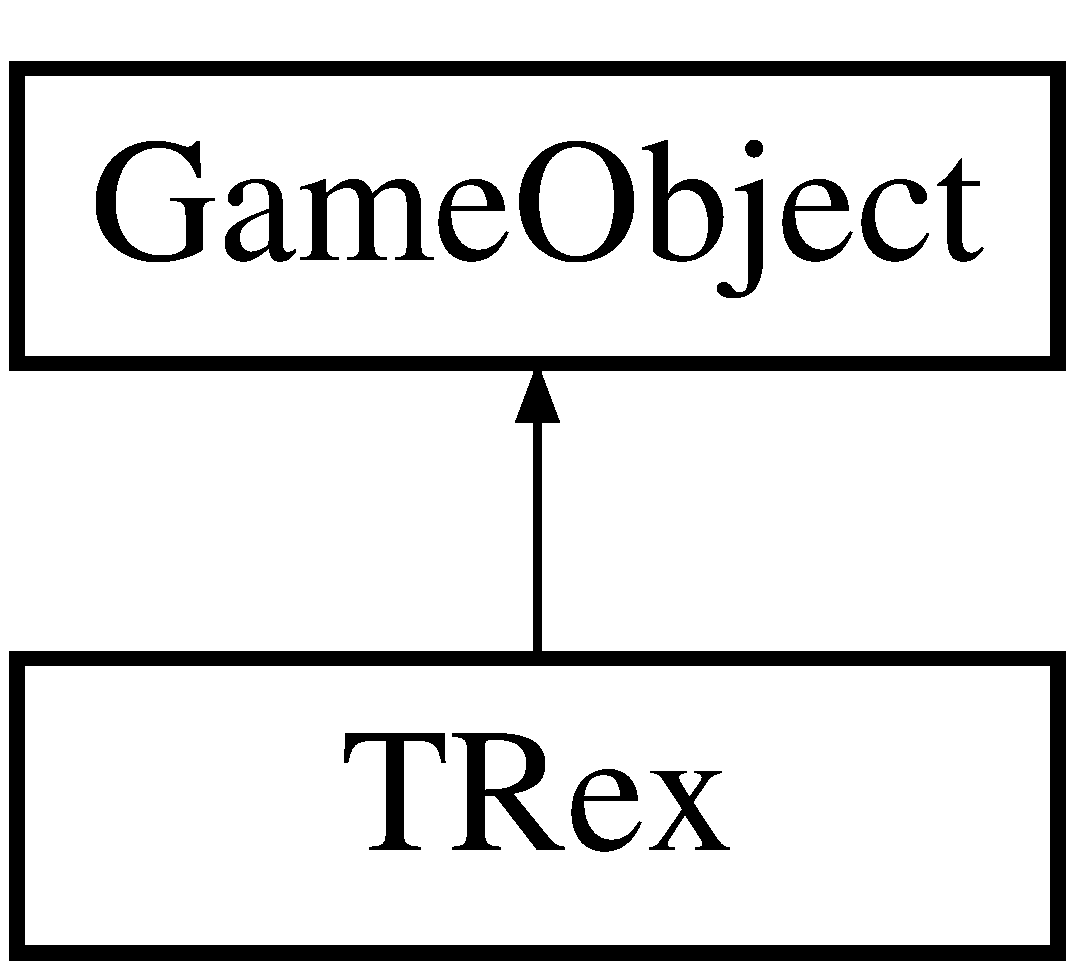
\includegraphics[height=2.000000cm]{class_t_rex}
\end{center}
\end{figure}
\subsection*{Public Types}
\begin{DoxyCompactItemize}
\item 
\mbox{\Hypertarget{class_t_rex_a000c4d51b41f07886af073a6b7b3e063}\label{class_t_rex_a000c4d51b41f07886af073a6b7b3e063}} 
enum {\bfseries T\+Rex\+States} \{ \newline
{\bfseries S\+T\+A\+N\+D\+I\+NG}, 
{\bfseries R\+U\+N\+N\+I\+N\+G1}, 
{\bfseries R\+U\+N\+N\+I\+N\+G2}, 
{\bfseries J\+U\+M\+P\+I\+NG}, 
\newline
{\bfseries D\+U\+C\+K\+I\+N\+G1}, 
{\bfseries D\+U\+C\+K\+I\+N\+G2}, 
{\bfseries C\+R\+A\+S\+H\+ED}
 \}
\end{DoxyCompactItemize}
\subsection*{Public Member Functions}
\begin{DoxyCompactItemize}
\item 
\mbox{\hyperlink{class_t_rex_ae762432f9b24294e971b9f62191f26e9}{T\+Rex}} (float jumping\+Speed, float gravity)
\begin{DoxyCompactList}\small\item\em \mbox{\hyperlink{class_t_rex}{T\+Rex}} constuctor. \end{DoxyCompactList}\item 
void \mbox{\hyperlink{class_t_rex_abc238b8e1df77d79f259cadd3a6c4cc8}{Jump}} ()
\begin{DoxyCompactList}\small\item\em Jump method. \end{DoxyCompactList}\item 
void \mbox{\hyperlink{class_t_rex_a1e672bcdbbeab5bc66c1812e3be30fd3}{Duck}} ()
\begin{DoxyCompactList}\small\item\em Duck method. \end{DoxyCompactList}\item 
void \mbox{\hyperlink{class_t_rex_af0e9ccbecc23739201a85e489da81efd}{Run}} ()
\begin{DoxyCompactList}\small\item\em Run method. \end{DoxyCompactList}\item 
\mbox{\Hypertarget{class_t_rex_a8881cde6c1a996532fa34cdb413ac441}\label{class_t_rex_a8881cde6c1a996532fa34cdb413ac441}} 
void \mbox{\hyperlink{class_t_rex_a8881cde6c1a996532fa34cdb413ac441}{Crash}} ()
\begin{DoxyCompactList}\small\item\em Crash method. \end{DoxyCompactList}\item 
void \mbox{\hyperlink{class_t_rex_aaef538213b79fb870e8af8f0cdf39a14}{Update}} ()
\begin{DoxyCompactList}\small\item\em Update method. \end{DoxyCompactList}\item 
\mbox{\Hypertarget{class_t_rex_a55dbaec9e6c442749133aaf017675c02}\label{class_t_rex_a55dbaec9e6c442749133aaf017675c02}} 
\mbox{\hyperlink{class_t_rex_a55dbaec9e6c442749133aaf017675c02}{$\sim$\+T\+Rex}} ()
\begin{DoxyCompactList}\small\item\em Default destructor. \end{DoxyCompactList}\end{DoxyCompactItemize}
\subsection*{Public Attributes}
\begin{DoxyCompactItemize}
\item 
\mbox{\Hypertarget{class_t_rex_ad30ad91fa9d6bb28c00e5d4819720d76}\label{class_t_rex_ad30ad91fa9d6bb28c00e5d4819720d76}} 
enum T\+Rex\+::\+T\+Rex\+States {\bfseries m\+\_\+state}
\end{DoxyCompactItemize}
\subsection*{Additional Inherited Members}


\subsection{Detailed Description}
\mbox{\hyperlink{_t_rex_8h_source}{T\+Rex.\+h}}. 

\mbox{\hyperlink{class_t_rex}{T\+Rex}} subclass

Created\+: 20.\+08.\+2018. Author \+: Robert Gerstmajer 

\subsection{Constructor \& Destructor Documentation}
\mbox{\Hypertarget{class_t_rex_ae762432f9b24294e971b9f62191f26e9}\label{class_t_rex_ae762432f9b24294e971b9f62191f26e9}} 
\index{T\+Rex@{T\+Rex}!T\+Rex@{T\+Rex}}
\index{T\+Rex@{T\+Rex}!T\+Rex@{T\+Rex}}
\subsubsection{\texorpdfstring{T\+Rex()}{TRex()}}
{\footnotesize\ttfamily T\+Rex\+::\+T\+Rex (\begin{DoxyParamCaption}\item[{float}]{jumping\+Speed,  }\item[{float}]{gravity }\end{DoxyParamCaption})}



\mbox{\hyperlink{class_t_rex}{T\+Rex}} constuctor. 

T\+Rex.\+cpp.


\begin{DoxyParams}{Parameters}
{\em jumping\+Speed} & loaded from config, how many pixels will the t\+Rex rise each frame \\
\hline
{\em gravity} & loaded from config, how many pixels will the t\+Rex drop each frame\\
\hline
\end{DoxyParams}
Implementation of the \mbox{\hyperlink{class_t_rex}{T\+Rex}} class

Created\+: 20.\+08.\+2018. Author \+: Robert Gerstmajer 

\subsection{Member Function Documentation}
\mbox{\Hypertarget{class_t_rex_a1e672bcdbbeab5bc66c1812e3be30fd3}\label{class_t_rex_a1e672bcdbbeab5bc66c1812e3be30fd3}} 
\index{T\+Rex@{T\+Rex}!Duck@{Duck}}
\index{Duck@{Duck}!T\+Rex@{T\+Rex}}
\subsubsection{\texorpdfstring{Duck()}{Duck()}}
{\footnotesize\ttfamily void T\+Rex\+::\+Duck (\begin{DoxyParamCaption}{ }\end{DoxyParamCaption})}



Duck method. 

Changes t\+Rex sprite to ducking, lowering its height \mbox{\Hypertarget{class_t_rex_abc238b8e1df77d79f259cadd3a6c4cc8}\label{class_t_rex_abc238b8e1df77d79f259cadd3a6c4cc8}} 
\index{T\+Rex@{T\+Rex}!Jump@{Jump}}
\index{Jump@{Jump}!T\+Rex@{T\+Rex}}
\subsubsection{\texorpdfstring{Jump()}{Jump()}}
{\footnotesize\ttfamily void T\+Rex\+::\+Jump (\begin{DoxyParamCaption}{ }\end{DoxyParamCaption})}



Jump method. 

Moves the t\+Rex up and drops it after reaching max height \mbox{\Hypertarget{class_t_rex_af0e9ccbecc23739201a85e489da81efd}\label{class_t_rex_af0e9ccbecc23739201a85e489da81efd}} 
\index{T\+Rex@{T\+Rex}!Run@{Run}}
\index{Run@{Run}!T\+Rex@{T\+Rex}}
\subsubsection{\texorpdfstring{Run()}{Run()}}
{\footnotesize\ttfamily void T\+Rex\+::\+Run (\begin{DoxyParamCaption}{ }\end{DoxyParamCaption})}



Run method. 

If the t\+Rex is jumping, do nothing; If the t\+Rex is on the ground or ducking, make it run normally \mbox{\Hypertarget{class_t_rex_aaef538213b79fb870e8af8f0cdf39a14}\label{class_t_rex_aaef538213b79fb870e8af8f0cdf39a14}} 
\index{T\+Rex@{T\+Rex}!Update@{Update}}
\index{Update@{Update}!T\+Rex@{T\+Rex}}
\subsubsection{\texorpdfstring{Update()}{Update()}}
{\footnotesize\ttfamily void T\+Rex\+::\+Update (\begin{DoxyParamCaption}{ }\end{DoxyParamCaption})}



Update method. 

If the t\+Rex is running or ducking, change sprites to look like it\textquotesingle{}s taking steps 

The documentation for this class was generated from the following files\+:\begin{DoxyCompactItemize}
\item 
T\+Rex.\+h\item 
T\+Rex.\+cpp\end{DoxyCompactItemize}

\hypertarget{classtinyxml2_1_1_x_m_l_attribute}{}\section{tinyxml2\+:\+:X\+M\+L\+Attribute Class Reference}
\label{classtinyxml2_1_1_x_m_l_attribute}\index{tinyxml2\+::\+X\+M\+L\+Attribute@{tinyxml2\+::\+X\+M\+L\+Attribute}}


{\ttfamily \#include $<$tinyxml2.\+h$>$}

\subsection*{Public Member Functions}
\begin{DoxyCompactItemize}
\item 
const char $\ast$ \mbox{\hyperlink{classtinyxml2_1_1_x_m_l_attribute_a5a5c135d24cce7abda6f17301c6274d8}{Name}} () const
\begin{DoxyCompactList}\small\item\em The name of the attribute. \end{DoxyCompactList}\item 
const char $\ast$ \mbox{\hyperlink{classtinyxml2_1_1_x_m_l_attribute_ab1c5cd993f836a771818ca408994b14e}{Value}} () const
\begin{DoxyCompactList}\small\item\em The value of the attribute. \end{DoxyCompactList}\item 
int \mbox{\hyperlink{classtinyxml2_1_1_x_m_l_attribute_a02d5ea924586e35f9c13857d1671b765}{Get\+Line\+Num}} () const
\begin{DoxyCompactList}\small\item\em Gets the line number the attribute is in, if the document was parsed from a file. \end{DoxyCompactList}\item 
const \mbox{\hyperlink{classtinyxml2_1_1_x_m_l_attribute}{X\+M\+L\+Attribute}} $\ast$ \mbox{\hyperlink{classtinyxml2_1_1_x_m_l_attribute_aee53571b21e7ce5421eb929523a8bbe6}{Next}} () const
\begin{DoxyCompactList}\small\item\em The next attribute in the list. \end{DoxyCompactList}\item 
int \mbox{\hyperlink{classtinyxml2_1_1_x_m_l_attribute_adfa2433f0fdafd5c3880936de9affa80}{Int\+Value}} () const
\item 
int64\+\_\+t \mbox{\hyperlink{classtinyxml2_1_1_x_m_l_attribute_a8762ed54f147c5744ada55c3d04d27f2}{Int64\+Value}} () const
\item 
unsigned \mbox{\hyperlink{classtinyxml2_1_1_x_m_l_attribute_a0be5343b08a957c42c02c5d32c35d338}{Unsigned\+Value}} () const
\begin{DoxyCompactList}\small\item\em Query as an unsigned integer. See \mbox{\hyperlink{classtinyxml2_1_1_x_m_l_attribute_adfa2433f0fdafd5c3880936de9affa80}{Int\+Value()}} \end{DoxyCompactList}\item 
bool \mbox{\hyperlink{classtinyxml2_1_1_x_m_l_attribute_a98ce5207344ad33a265b0422addae1ff}{Bool\+Value}} () const
\begin{DoxyCompactList}\small\item\em Query as a boolean. See \mbox{\hyperlink{classtinyxml2_1_1_x_m_l_attribute_adfa2433f0fdafd5c3880936de9affa80}{Int\+Value()}} \end{DoxyCompactList}\item 
double \mbox{\hyperlink{classtinyxml2_1_1_x_m_l_attribute_a4aa73513f54ff0087d3e804f0f54e30f}{Double\+Value}} () const
\begin{DoxyCompactList}\small\item\em Query as a double. See \mbox{\hyperlink{classtinyxml2_1_1_x_m_l_attribute_adfa2433f0fdafd5c3880936de9affa80}{Int\+Value()}} \end{DoxyCompactList}\item 
float \mbox{\hyperlink{classtinyxml2_1_1_x_m_l_attribute_a27797b45d21c981257720db94f5f8801}{Float\+Value}} () const
\begin{DoxyCompactList}\small\item\em Query as a float. See \mbox{\hyperlink{classtinyxml2_1_1_x_m_l_attribute_adfa2433f0fdafd5c3880936de9affa80}{Int\+Value()}} \end{DoxyCompactList}\item 
\mbox{\hyperlink{namespacetinyxml2_a1fbf88509c3ac88c09117b1947414e08}{X\+M\+L\+Error}} \mbox{\hyperlink{classtinyxml2_1_1_x_m_l_attribute_a6d5176260db00ea301c01af8457cd993}{Query\+Int\+Value}} (int $\ast$value) const
\item 
\mbox{\hyperlink{namespacetinyxml2_a1fbf88509c3ac88c09117b1947414e08}{X\+M\+L\+Error}} \mbox{\hyperlink{classtinyxml2_1_1_x_m_l_attribute_a48a7f3496f1415832e451bd8d09c9cb9}{Query\+Unsigned\+Value}} (unsigned int $\ast$value) const
\begin{DoxyCompactList}\small\item\em See Query\+Int\+Value. \end{DoxyCompactList}\item 
\mbox{\hyperlink{namespacetinyxml2_a1fbf88509c3ac88c09117b1947414e08}{X\+M\+L\+Error}} \mbox{\hyperlink{classtinyxml2_1_1_x_m_l_attribute_a4e25344d6e4159026be34dbddf1dcac2}{Query\+Int64\+Value}} (int64\+\_\+t $\ast$value) const
\begin{DoxyCompactList}\small\item\em See Query\+Int\+Value. \end{DoxyCompactList}\item 
\mbox{\hyperlink{namespacetinyxml2_a1fbf88509c3ac88c09117b1947414e08}{X\+M\+L\+Error}} \mbox{\hyperlink{classtinyxml2_1_1_x_m_l_attribute_a5f32e038954256f61c21ff20fd13a09c}{Query\+Bool\+Value}} (bool $\ast$value) const
\begin{DoxyCompactList}\small\item\em See Query\+Int\+Value. \end{DoxyCompactList}\item 
\mbox{\hyperlink{namespacetinyxml2_a1fbf88509c3ac88c09117b1947414e08}{X\+M\+L\+Error}} \mbox{\hyperlink{classtinyxml2_1_1_x_m_l_attribute_a2aa6e55e8ea03af0609cf6690bff79b9}{Query\+Double\+Value}} (double $\ast$value) const
\begin{DoxyCompactList}\small\item\em See Query\+Int\+Value. \end{DoxyCompactList}\item 
\mbox{\hyperlink{namespacetinyxml2_a1fbf88509c3ac88c09117b1947414e08}{X\+M\+L\+Error}} \mbox{\hyperlink{classtinyxml2_1_1_x_m_l_attribute_a049dea6449a6259b6cfed44a9427b607}{Query\+Float\+Value}} (float $\ast$value) const
\begin{DoxyCompactList}\small\item\em See Query\+Int\+Value. \end{DoxyCompactList}\item 
void \mbox{\hyperlink{classtinyxml2_1_1_x_m_l_attribute_a406d2c4a13c7af99a65edb59dd9f7581}{Set\+Attribute}} (const char $\ast$value)
\begin{DoxyCompactList}\small\item\em Set the attribute to a string value. \end{DoxyCompactList}\item 
void \mbox{\hyperlink{classtinyxml2_1_1_x_m_l_attribute_ad86d7d7058d76761c3a80662566a57e5}{Set\+Attribute}} (int value)
\begin{DoxyCompactList}\small\item\em Set the attribute to value. \end{DoxyCompactList}\item 
void \mbox{\hyperlink{classtinyxml2_1_1_x_m_l_attribute_ae70468c0f6df2748ba3529c716999fae}{Set\+Attribute}} (unsigned value)
\begin{DoxyCompactList}\small\item\em Set the attribute to value. \end{DoxyCompactList}\item 
void \mbox{\hyperlink{classtinyxml2_1_1_x_m_l_attribute_a7c1240f479722b9aa29b6c030aa116c2}{Set\+Attribute}} (int64\+\_\+t value)
\begin{DoxyCompactList}\small\item\em Set the attribute to value. \end{DoxyCompactList}\item 
void \mbox{\hyperlink{classtinyxml2_1_1_x_m_l_attribute_ab3516def4fe058fe328f2b89fc2d77da}{Set\+Attribute}} (bool value)
\begin{DoxyCompactList}\small\item\em Set the attribute to value. \end{DoxyCompactList}\item 
void \mbox{\hyperlink{classtinyxml2_1_1_x_m_l_attribute_a9a65ab3147abe8ccbbd373ce8791e818}{Set\+Attribute}} (double value)
\begin{DoxyCompactList}\small\item\em Set the attribute to value. \end{DoxyCompactList}\item 
void \mbox{\hyperlink{classtinyxml2_1_1_x_m_l_attribute_ae95e843313aaf5d56c32530b6456df02}{Set\+Attribute}} (float value)
\begin{DoxyCompactList}\small\item\em Set the attribute to value. \end{DoxyCompactList}\end{DoxyCompactItemize}
\subsection*{Friends}
\begin{DoxyCompactItemize}
\item 
class \mbox{\hyperlink{classtinyxml2_1_1_x_m_l_attribute_ac2fba9b6e452829dd892f7392c24e0eb}{X\+M\+L\+Element}}
\end{DoxyCompactItemize}


\subsection{Detailed Description}
An attribute is a name-\/value pair. Elements have an arbitrary number of attributes, each with a unique name.

\begin{DoxyNote}{Note}
The attributes are not X\+M\+L\+Nodes. You may only query the \mbox{\hyperlink{classtinyxml2_1_1_x_m_l_attribute_aee53571b21e7ce5421eb929523a8bbe6}{Next()}} attribute in a list. 
\end{DoxyNote}


\subsection{Member Function Documentation}
\mbox{\Hypertarget{classtinyxml2_1_1_x_m_l_attribute_a98ce5207344ad33a265b0422addae1ff}\label{classtinyxml2_1_1_x_m_l_attribute_a98ce5207344ad33a265b0422addae1ff}} 
\index{tinyxml2\+::\+X\+M\+L\+Attribute@{tinyxml2\+::\+X\+M\+L\+Attribute}!Bool\+Value@{Bool\+Value}}
\index{Bool\+Value@{Bool\+Value}!tinyxml2\+::\+X\+M\+L\+Attribute@{tinyxml2\+::\+X\+M\+L\+Attribute}}
\subsubsection{\texorpdfstring{Bool\+Value()}{BoolValue()}}
{\footnotesize\ttfamily bool tinyxml2\+::\+X\+M\+L\+Attribute\+::\+Bool\+Value (\begin{DoxyParamCaption}{ }\end{DoxyParamCaption}) const\hspace{0.3cm}{\ttfamily [inline]}}



Query as a boolean. See \mbox{\hyperlink{classtinyxml2_1_1_x_m_l_attribute_adfa2433f0fdafd5c3880936de9affa80}{Int\+Value()}} 

\mbox{\Hypertarget{classtinyxml2_1_1_x_m_l_attribute_a4aa73513f54ff0087d3e804f0f54e30f}\label{classtinyxml2_1_1_x_m_l_attribute_a4aa73513f54ff0087d3e804f0f54e30f}} 
\index{tinyxml2\+::\+X\+M\+L\+Attribute@{tinyxml2\+::\+X\+M\+L\+Attribute}!Double\+Value@{Double\+Value}}
\index{Double\+Value@{Double\+Value}!tinyxml2\+::\+X\+M\+L\+Attribute@{tinyxml2\+::\+X\+M\+L\+Attribute}}
\subsubsection{\texorpdfstring{Double\+Value()}{DoubleValue()}}
{\footnotesize\ttfamily double tinyxml2\+::\+X\+M\+L\+Attribute\+::\+Double\+Value (\begin{DoxyParamCaption}{ }\end{DoxyParamCaption}) const\hspace{0.3cm}{\ttfamily [inline]}}



Query as a double. See \mbox{\hyperlink{classtinyxml2_1_1_x_m_l_attribute_adfa2433f0fdafd5c3880936de9affa80}{Int\+Value()}} 

\mbox{\Hypertarget{classtinyxml2_1_1_x_m_l_attribute_a27797b45d21c981257720db94f5f8801}\label{classtinyxml2_1_1_x_m_l_attribute_a27797b45d21c981257720db94f5f8801}} 
\index{tinyxml2\+::\+X\+M\+L\+Attribute@{tinyxml2\+::\+X\+M\+L\+Attribute}!Float\+Value@{Float\+Value}}
\index{Float\+Value@{Float\+Value}!tinyxml2\+::\+X\+M\+L\+Attribute@{tinyxml2\+::\+X\+M\+L\+Attribute}}
\subsubsection{\texorpdfstring{Float\+Value()}{FloatValue()}}
{\footnotesize\ttfamily float tinyxml2\+::\+X\+M\+L\+Attribute\+::\+Float\+Value (\begin{DoxyParamCaption}{ }\end{DoxyParamCaption}) const\hspace{0.3cm}{\ttfamily [inline]}}



Query as a float. See \mbox{\hyperlink{classtinyxml2_1_1_x_m_l_attribute_adfa2433f0fdafd5c3880936de9affa80}{Int\+Value()}} 

\mbox{\Hypertarget{classtinyxml2_1_1_x_m_l_attribute_a02d5ea924586e35f9c13857d1671b765}\label{classtinyxml2_1_1_x_m_l_attribute_a02d5ea924586e35f9c13857d1671b765}} 
\index{tinyxml2\+::\+X\+M\+L\+Attribute@{tinyxml2\+::\+X\+M\+L\+Attribute}!Get\+Line\+Num@{Get\+Line\+Num}}
\index{Get\+Line\+Num@{Get\+Line\+Num}!tinyxml2\+::\+X\+M\+L\+Attribute@{tinyxml2\+::\+X\+M\+L\+Attribute}}
\subsubsection{\texorpdfstring{Get\+Line\+Num()}{GetLineNum()}}
{\footnotesize\ttfamily int tinyxml2\+::\+X\+M\+L\+Attribute\+::\+Get\+Line\+Num (\begin{DoxyParamCaption}{ }\end{DoxyParamCaption}) const\hspace{0.3cm}{\ttfamily [inline]}}



Gets the line number the attribute is in, if the document was parsed from a file. 

\mbox{\Hypertarget{classtinyxml2_1_1_x_m_l_attribute_a8762ed54f147c5744ada55c3d04d27f2}\label{classtinyxml2_1_1_x_m_l_attribute_a8762ed54f147c5744ada55c3d04d27f2}} 
\index{tinyxml2\+::\+X\+M\+L\+Attribute@{tinyxml2\+::\+X\+M\+L\+Attribute}!Int64\+Value@{Int64\+Value}}
\index{Int64\+Value@{Int64\+Value}!tinyxml2\+::\+X\+M\+L\+Attribute@{tinyxml2\+::\+X\+M\+L\+Attribute}}
\subsubsection{\texorpdfstring{Int64\+Value()}{Int64Value()}}
{\footnotesize\ttfamily int64\+\_\+t tinyxml2\+::\+X\+M\+L\+Attribute\+::\+Int64\+Value (\begin{DoxyParamCaption}{ }\end{DoxyParamCaption}) const\hspace{0.3cm}{\ttfamily [inline]}}

\mbox{\Hypertarget{classtinyxml2_1_1_x_m_l_attribute_adfa2433f0fdafd5c3880936de9affa80}\label{classtinyxml2_1_1_x_m_l_attribute_adfa2433f0fdafd5c3880936de9affa80}} 
\index{tinyxml2\+::\+X\+M\+L\+Attribute@{tinyxml2\+::\+X\+M\+L\+Attribute}!Int\+Value@{Int\+Value}}
\index{Int\+Value@{Int\+Value}!tinyxml2\+::\+X\+M\+L\+Attribute@{tinyxml2\+::\+X\+M\+L\+Attribute}}
\subsubsection{\texorpdfstring{Int\+Value()}{IntValue()}}
{\footnotesize\ttfamily int tinyxml2\+::\+X\+M\+L\+Attribute\+::\+Int\+Value (\begin{DoxyParamCaption}{ }\end{DoxyParamCaption}) const\hspace{0.3cm}{\ttfamily [inline]}}

Int\+Value interprets the attribute as an integer, and returns the value. If the value isn\textquotesingle{}t an integer, 0 will be returned. There is no error checking; use \mbox{\hyperlink{classtinyxml2_1_1_x_m_l_attribute_a6d5176260db00ea301c01af8457cd993}{Query\+Int\+Value()}} if you need error checking. \mbox{\Hypertarget{classtinyxml2_1_1_x_m_l_attribute_a5a5c135d24cce7abda6f17301c6274d8}\label{classtinyxml2_1_1_x_m_l_attribute_a5a5c135d24cce7abda6f17301c6274d8}} 
\index{tinyxml2\+::\+X\+M\+L\+Attribute@{tinyxml2\+::\+X\+M\+L\+Attribute}!Name@{Name}}
\index{Name@{Name}!tinyxml2\+::\+X\+M\+L\+Attribute@{tinyxml2\+::\+X\+M\+L\+Attribute}}
\subsubsection{\texorpdfstring{Name()}{Name()}}
{\footnotesize\ttfamily const char $\ast$ tinyxml2\+::\+X\+M\+L\+Attribute\+::\+Name (\begin{DoxyParamCaption}{ }\end{DoxyParamCaption}) const}



The name of the attribute. 

\mbox{\Hypertarget{classtinyxml2_1_1_x_m_l_attribute_aee53571b21e7ce5421eb929523a8bbe6}\label{classtinyxml2_1_1_x_m_l_attribute_aee53571b21e7ce5421eb929523a8bbe6}} 
\index{tinyxml2\+::\+X\+M\+L\+Attribute@{tinyxml2\+::\+X\+M\+L\+Attribute}!Next@{Next}}
\index{Next@{Next}!tinyxml2\+::\+X\+M\+L\+Attribute@{tinyxml2\+::\+X\+M\+L\+Attribute}}
\subsubsection{\texorpdfstring{Next()}{Next()}}
{\footnotesize\ttfamily const \mbox{\hyperlink{classtinyxml2_1_1_x_m_l_attribute}{X\+M\+L\+Attribute}}$\ast$ tinyxml2\+::\+X\+M\+L\+Attribute\+::\+Next (\begin{DoxyParamCaption}{ }\end{DoxyParamCaption}) const\hspace{0.3cm}{\ttfamily [inline]}}



The next attribute in the list. 

\mbox{\Hypertarget{classtinyxml2_1_1_x_m_l_attribute_a5f32e038954256f61c21ff20fd13a09c}\label{classtinyxml2_1_1_x_m_l_attribute_a5f32e038954256f61c21ff20fd13a09c}} 
\index{tinyxml2\+::\+X\+M\+L\+Attribute@{tinyxml2\+::\+X\+M\+L\+Attribute}!Query\+Bool\+Value@{Query\+Bool\+Value}}
\index{Query\+Bool\+Value@{Query\+Bool\+Value}!tinyxml2\+::\+X\+M\+L\+Attribute@{tinyxml2\+::\+X\+M\+L\+Attribute}}
\subsubsection{\texorpdfstring{Query\+Bool\+Value()}{QueryBoolValue()}}
{\footnotesize\ttfamily \mbox{\hyperlink{namespacetinyxml2_a1fbf88509c3ac88c09117b1947414e08}{X\+M\+L\+Error}} tinyxml2\+::\+X\+M\+L\+Attribute\+::\+Query\+Bool\+Value (\begin{DoxyParamCaption}\item[{bool $\ast$}]{value }\end{DoxyParamCaption}) const}



See Query\+Int\+Value. 

\mbox{\Hypertarget{classtinyxml2_1_1_x_m_l_attribute_a2aa6e55e8ea03af0609cf6690bff79b9}\label{classtinyxml2_1_1_x_m_l_attribute_a2aa6e55e8ea03af0609cf6690bff79b9}} 
\index{tinyxml2\+::\+X\+M\+L\+Attribute@{tinyxml2\+::\+X\+M\+L\+Attribute}!Query\+Double\+Value@{Query\+Double\+Value}}
\index{Query\+Double\+Value@{Query\+Double\+Value}!tinyxml2\+::\+X\+M\+L\+Attribute@{tinyxml2\+::\+X\+M\+L\+Attribute}}
\subsubsection{\texorpdfstring{Query\+Double\+Value()}{QueryDoubleValue()}}
{\footnotesize\ttfamily \mbox{\hyperlink{namespacetinyxml2_a1fbf88509c3ac88c09117b1947414e08}{X\+M\+L\+Error}} tinyxml2\+::\+X\+M\+L\+Attribute\+::\+Query\+Double\+Value (\begin{DoxyParamCaption}\item[{double $\ast$}]{value }\end{DoxyParamCaption}) const}



See Query\+Int\+Value. 

\mbox{\Hypertarget{classtinyxml2_1_1_x_m_l_attribute_a049dea6449a6259b6cfed44a9427b607}\label{classtinyxml2_1_1_x_m_l_attribute_a049dea6449a6259b6cfed44a9427b607}} 
\index{tinyxml2\+::\+X\+M\+L\+Attribute@{tinyxml2\+::\+X\+M\+L\+Attribute}!Query\+Float\+Value@{Query\+Float\+Value}}
\index{Query\+Float\+Value@{Query\+Float\+Value}!tinyxml2\+::\+X\+M\+L\+Attribute@{tinyxml2\+::\+X\+M\+L\+Attribute}}
\subsubsection{\texorpdfstring{Query\+Float\+Value()}{QueryFloatValue()}}
{\footnotesize\ttfamily \mbox{\hyperlink{namespacetinyxml2_a1fbf88509c3ac88c09117b1947414e08}{X\+M\+L\+Error}} tinyxml2\+::\+X\+M\+L\+Attribute\+::\+Query\+Float\+Value (\begin{DoxyParamCaption}\item[{float $\ast$}]{value }\end{DoxyParamCaption}) const}



See Query\+Int\+Value. 

\mbox{\Hypertarget{classtinyxml2_1_1_x_m_l_attribute_a4e25344d6e4159026be34dbddf1dcac2}\label{classtinyxml2_1_1_x_m_l_attribute_a4e25344d6e4159026be34dbddf1dcac2}} 
\index{tinyxml2\+::\+X\+M\+L\+Attribute@{tinyxml2\+::\+X\+M\+L\+Attribute}!Query\+Int64\+Value@{Query\+Int64\+Value}}
\index{Query\+Int64\+Value@{Query\+Int64\+Value}!tinyxml2\+::\+X\+M\+L\+Attribute@{tinyxml2\+::\+X\+M\+L\+Attribute}}
\subsubsection{\texorpdfstring{Query\+Int64\+Value()}{QueryInt64Value()}}
{\footnotesize\ttfamily \mbox{\hyperlink{namespacetinyxml2_a1fbf88509c3ac88c09117b1947414e08}{X\+M\+L\+Error}} tinyxml2\+::\+X\+M\+L\+Attribute\+::\+Query\+Int64\+Value (\begin{DoxyParamCaption}\item[{int64\+\_\+t $\ast$}]{value }\end{DoxyParamCaption}) const}



See Query\+Int\+Value. 

\mbox{\Hypertarget{classtinyxml2_1_1_x_m_l_attribute_a6d5176260db00ea301c01af8457cd993}\label{classtinyxml2_1_1_x_m_l_attribute_a6d5176260db00ea301c01af8457cd993}} 
\index{tinyxml2\+::\+X\+M\+L\+Attribute@{tinyxml2\+::\+X\+M\+L\+Attribute}!Query\+Int\+Value@{Query\+Int\+Value}}
\index{Query\+Int\+Value@{Query\+Int\+Value}!tinyxml2\+::\+X\+M\+L\+Attribute@{tinyxml2\+::\+X\+M\+L\+Attribute}}
\subsubsection{\texorpdfstring{Query\+Int\+Value()}{QueryIntValue()}}
{\footnotesize\ttfamily \mbox{\hyperlink{namespacetinyxml2_a1fbf88509c3ac88c09117b1947414e08}{X\+M\+L\+Error}} tinyxml2\+::\+X\+M\+L\+Attribute\+::\+Query\+Int\+Value (\begin{DoxyParamCaption}\item[{int $\ast$}]{value }\end{DoxyParamCaption}) const}

Query\+Int\+Value interprets the attribute as an integer, and returns the value in the provided parameter. The function will return X\+M\+L\+\_\+\+S\+U\+C\+C\+E\+SS on success, and X\+M\+L\+\_\+\+W\+R\+O\+N\+G\+\_\+\+A\+T\+T\+R\+I\+B\+U\+T\+E\+\_\+\+T\+Y\+PE if the conversion is not successful. \mbox{\Hypertarget{classtinyxml2_1_1_x_m_l_attribute_a48a7f3496f1415832e451bd8d09c9cb9}\label{classtinyxml2_1_1_x_m_l_attribute_a48a7f3496f1415832e451bd8d09c9cb9}} 
\index{tinyxml2\+::\+X\+M\+L\+Attribute@{tinyxml2\+::\+X\+M\+L\+Attribute}!Query\+Unsigned\+Value@{Query\+Unsigned\+Value}}
\index{Query\+Unsigned\+Value@{Query\+Unsigned\+Value}!tinyxml2\+::\+X\+M\+L\+Attribute@{tinyxml2\+::\+X\+M\+L\+Attribute}}
\subsubsection{\texorpdfstring{Query\+Unsigned\+Value()}{QueryUnsignedValue()}}
{\footnotesize\ttfamily \mbox{\hyperlink{namespacetinyxml2_a1fbf88509c3ac88c09117b1947414e08}{X\+M\+L\+Error}} tinyxml2\+::\+X\+M\+L\+Attribute\+::\+Query\+Unsigned\+Value (\begin{DoxyParamCaption}\item[{unsigned int $\ast$}]{value }\end{DoxyParamCaption}) const}



See Query\+Int\+Value. 

\mbox{\Hypertarget{classtinyxml2_1_1_x_m_l_attribute_a406d2c4a13c7af99a65edb59dd9f7581}\label{classtinyxml2_1_1_x_m_l_attribute_a406d2c4a13c7af99a65edb59dd9f7581}} 
\index{tinyxml2\+::\+X\+M\+L\+Attribute@{tinyxml2\+::\+X\+M\+L\+Attribute}!Set\+Attribute@{Set\+Attribute}}
\index{Set\+Attribute@{Set\+Attribute}!tinyxml2\+::\+X\+M\+L\+Attribute@{tinyxml2\+::\+X\+M\+L\+Attribute}}
\subsubsection{\texorpdfstring{Set\+Attribute()}{SetAttribute()}\hspace{0.1cm}{\footnotesize\ttfamily [1/7]}}
{\footnotesize\ttfamily void tinyxml2\+::\+X\+M\+L\+Attribute\+::\+Set\+Attribute (\begin{DoxyParamCaption}\item[{const char $\ast$}]{value }\end{DoxyParamCaption})}



Set the attribute to a string value. 

\mbox{\Hypertarget{classtinyxml2_1_1_x_m_l_attribute_ad86d7d7058d76761c3a80662566a57e5}\label{classtinyxml2_1_1_x_m_l_attribute_ad86d7d7058d76761c3a80662566a57e5}} 
\index{tinyxml2\+::\+X\+M\+L\+Attribute@{tinyxml2\+::\+X\+M\+L\+Attribute}!Set\+Attribute@{Set\+Attribute}}
\index{Set\+Attribute@{Set\+Attribute}!tinyxml2\+::\+X\+M\+L\+Attribute@{tinyxml2\+::\+X\+M\+L\+Attribute}}
\subsubsection{\texorpdfstring{Set\+Attribute()}{SetAttribute()}\hspace{0.1cm}{\footnotesize\ttfamily [2/7]}}
{\footnotesize\ttfamily void tinyxml2\+::\+X\+M\+L\+Attribute\+::\+Set\+Attribute (\begin{DoxyParamCaption}\item[{int}]{value }\end{DoxyParamCaption})}



Set the attribute to value. 

\mbox{\Hypertarget{classtinyxml2_1_1_x_m_l_attribute_ae70468c0f6df2748ba3529c716999fae}\label{classtinyxml2_1_1_x_m_l_attribute_ae70468c0f6df2748ba3529c716999fae}} 
\index{tinyxml2\+::\+X\+M\+L\+Attribute@{tinyxml2\+::\+X\+M\+L\+Attribute}!Set\+Attribute@{Set\+Attribute}}
\index{Set\+Attribute@{Set\+Attribute}!tinyxml2\+::\+X\+M\+L\+Attribute@{tinyxml2\+::\+X\+M\+L\+Attribute}}
\subsubsection{\texorpdfstring{Set\+Attribute()}{SetAttribute()}\hspace{0.1cm}{\footnotesize\ttfamily [3/7]}}
{\footnotesize\ttfamily void tinyxml2\+::\+X\+M\+L\+Attribute\+::\+Set\+Attribute (\begin{DoxyParamCaption}\item[{unsigned}]{value }\end{DoxyParamCaption})}



Set the attribute to value. 

\mbox{\Hypertarget{classtinyxml2_1_1_x_m_l_attribute_a7c1240f479722b9aa29b6c030aa116c2}\label{classtinyxml2_1_1_x_m_l_attribute_a7c1240f479722b9aa29b6c030aa116c2}} 
\index{tinyxml2\+::\+X\+M\+L\+Attribute@{tinyxml2\+::\+X\+M\+L\+Attribute}!Set\+Attribute@{Set\+Attribute}}
\index{Set\+Attribute@{Set\+Attribute}!tinyxml2\+::\+X\+M\+L\+Attribute@{tinyxml2\+::\+X\+M\+L\+Attribute}}
\subsubsection{\texorpdfstring{Set\+Attribute()}{SetAttribute()}\hspace{0.1cm}{\footnotesize\ttfamily [4/7]}}
{\footnotesize\ttfamily void tinyxml2\+::\+X\+M\+L\+Attribute\+::\+Set\+Attribute (\begin{DoxyParamCaption}\item[{int64\+\_\+t}]{value }\end{DoxyParamCaption})}



Set the attribute to value. 

\mbox{\Hypertarget{classtinyxml2_1_1_x_m_l_attribute_ab3516def4fe058fe328f2b89fc2d77da}\label{classtinyxml2_1_1_x_m_l_attribute_ab3516def4fe058fe328f2b89fc2d77da}} 
\index{tinyxml2\+::\+X\+M\+L\+Attribute@{tinyxml2\+::\+X\+M\+L\+Attribute}!Set\+Attribute@{Set\+Attribute}}
\index{Set\+Attribute@{Set\+Attribute}!tinyxml2\+::\+X\+M\+L\+Attribute@{tinyxml2\+::\+X\+M\+L\+Attribute}}
\subsubsection{\texorpdfstring{Set\+Attribute()}{SetAttribute()}\hspace{0.1cm}{\footnotesize\ttfamily [5/7]}}
{\footnotesize\ttfamily void tinyxml2\+::\+X\+M\+L\+Attribute\+::\+Set\+Attribute (\begin{DoxyParamCaption}\item[{bool}]{value }\end{DoxyParamCaption})}



Set the attribute to value. 

\mbox{\Hypertarget{classtinyxml2_1_1_x_m_l_attribute_a9a65ab3147abe8ccbbd373ce8791e818}\label{classtinyxml2_1_1_x_m_l_attribute_a9a65ab3147abe8ccbbd373ce8791e818}} 
\index{tinyxml2\+::\+X\+M\+L\+Attribute@{tinyxml2\+::\+X\+M\+L\+Attribute}!Set\+Attribute@{Set\+Attribute}}
\index{Set\+Attribute@{Set\+Attribute}!tinyxml2\+::\+X\+M\+L\+Attribute@{tinyxml2\+::\+X\+M\+L\+Attribute}}
\subsubsection{\texorpdfstring{Set\+Attribute()}{SetAttribute()}\hspace{0.1cm}{\footnotesize\ttfamily [6/7]}}
{\footnotesize\ttfamily void tinyxml2\+::\+X\+M\+L\+Attribute\+::\+Set\+Attribute (\begin{DoxyParamCaption}\item[{double}]{value }\end{DoxyParamCaption})}



Set the attribute to value. 

\mbox{\Hypertarget{classtinyxml2_1_1_x_m_l_attribute_ae95e843313aaf5d56c32530b6456df02}\label{classtinyxml2_1_1_x_m_l_attribute_ae95e843313aaf5d56c32530b6456df02}} 
\index{tinyxml2\+::\+X\+M\+L\+Attribute@{tinyxml2\+::\+X\+M\+L\+Attribute}!Set\+Attribute@{Set\+Attribute}}
\index{Set\+Attribute@{Set\+Attribute}!tinyxml2\+::\+X\+M\+L\+Attribute@{tinyxml2\+::\+X\+M\+L\+Attribute}}
\subsubsection{\texorpdfstring{Set\+Attribute()}{SetAttribute()}\hspace{0.1cm}{\footnotesize\ttfamily [7/7]}}
{\footnotesize\ttfamily void tinyxml2\+::\+X\+M\+L\+Attribute\+::\+Set\+Attribute (\begin{DoxyParamCaption}\item[{float}]{value }\end{DoxyParamCaption})}



Set the attribute to value. 

\mbox{\Hypertarget{classtinyxml2_1_1_x_m_l_attribute_a0be5343b08a957c42c02c5d32c35d338}\label{classtinyxml2_1_1_x_m_l_attribute_a0be5343b08a957c42c02c5d32c35d338}} 
\index{tinyxml2\+::\+X\+M\+L\+Attribute@{tinyxml2\+::\+X\+M\+L\+Attribute}!Unsigned\+Value@{Unsigned\+Value}}
\index{Unsigned\+Value@{Unsigned\+Value}!tinyxml2\+::\+X\+M\+L\+Attribute@{tinyxml2\+::\+X\+M\+L\+Attribute}}
\subsubsection{\texorpdfstring{Unsigned\+Value()}{UnsignedValue()}}
{\footnotesize\ttfamily unsigned tinyxml2\+::\+X\+M\+L\+Attribute\+::\+Unsigned\+Value (\begin{DoxyParamCaption}{ }\end{DoxyParamCaption}) const\hspace{0.3cm}{\ttfamily [inline]}}



Query as an unsigned integer. See \mbox{\hyperlink{classtinyxml2_1_1_x_m_l_attribute_adfa2433f0fdafd5c3880936de9affa80}{Int\+Value()}} 

\mbox{\Hypertarget{classtinyxml2_1_1_x_m_l_attribute_ab1c5cd993f836a771818ca408994b14e}\label{classtinyxml2_1_1_x_m_l_attribute_ab1c5cd993f836a771818ca408994b14e}} 
\index{tinyxml2\+::\+X\+M\+L\+Attribute@{tinyxml2\+::\+X\+M\+L\+Attribute}!Value@{Value}}
\index{Value@{Value}!tinyxml2\+::\+X\+M\+L\+Attribute@{tinyxml2\+::\+X\+M\+L\+Attribute}}
\subsubsection{\texorpdfstring{Value()}{Value()}}
{\footnotesize\ttfamily const char $\ast$ tinyxml2\+::\+X\+M\+L\+Attribute\+::\+Value (\begin{DoxyParamCaption}{ }\end{DoxyParamCaption}) const}



The value of the attribute. 



\subsection{Friends And Related Function Documentation}
\mbox{\Hypertarget{classtinyxml2_1_1_x_m_l_attribute_ac2fba9b6e452829dd892f7392c24e0eb}\label{classtinyxml2_1_1_x_m_l_attribute_ac2fba9b6e452829dd892f7392c24e0eb}} 
\index{tinyxml2\+::\+X\+M\+L\+Attribute@{tinyxml2\+::\+X\+M\+L\+Attribute}!X\+M\+L\+Element@{X\+M\+L\+Element}}
\index{X\+M\+L\+Element@{X\+M\+L\+Element}!tinyxml2\+::\+X\+M\+L\+Attribute@{tinyxml2\+::\+X\+M\+L\+Attribute}}
\subsubsection{\texorpdfstring{X\+M\+L\+Element}{XMLElement}}
{\footnotesize\ttfamily friend class \mbox{\hyperlink{classtinyxml2_1_1_x_m_l_element}{X\+M\+L\+Element}}\hspace{0.3cm}{\ttfamily [friend]}}



The documentation for this class was generated from the following files\+:\begin{DoxyCompactItemize}
\item 
\mbox{\hyperlink{tinyxml2_8h}{tinyxml2.\+h}}\item 
\mbox{\hyperlink{tinyxml2_8cpp}{tinyxml2.\+cpp}}\end{DoxyCompactItemize}

\hypertarget{classtinyxml2_1_1_x_m_l_comment}{}\section{tinyxml2\+:\+:X\+M\+L\+Comment Class Reference}
\label{classtinyxml2_1_1_x_m_l_comment}\index{tinyxml2\+::\+X\+M\+L\+Comment@{tinyxml2\+::\+X\+M\+L\+Comment}}


{\ttfamily \#include $<$tinyxml2.\+h$>$}

Inheritance diagram for tinyxml2\+:\+:X\+M\+L\+Comment\+:\begin{figure}[H]
\begin{center}
\leavevmode
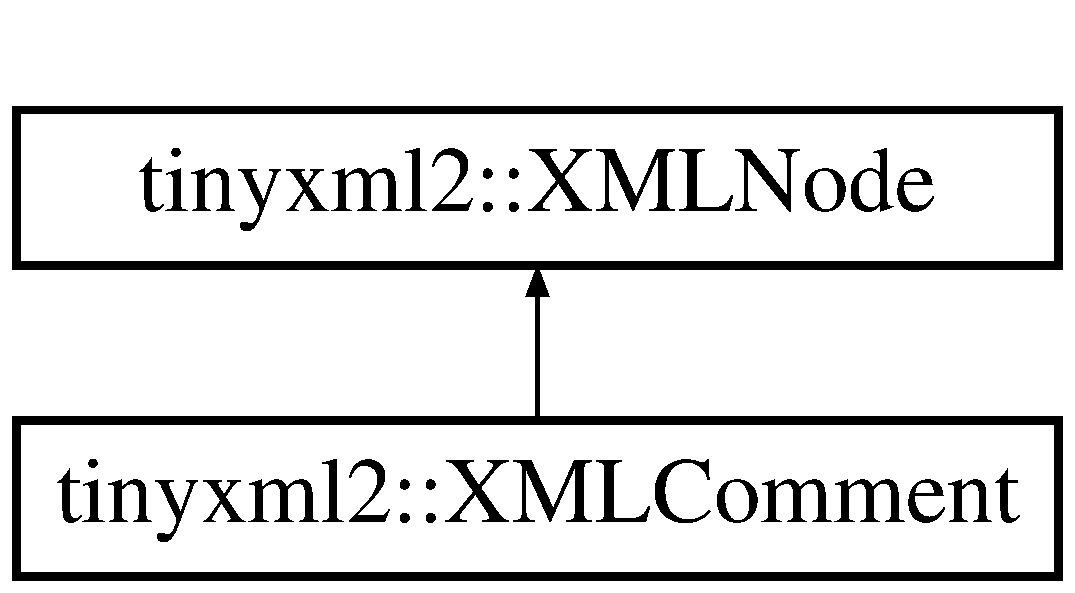
\includegraphics[height=2.000000cm]{classtinyxml2_1_1_x_m_l_comment}
\end{center}
\end{figure}
\subsection*{Public Member Functions}
\begin{DoxyCompactItemize}
\item 
virtual \mbox{\hyperlink{classtinyxml2_1_1_x_m_l_comment}{X\+M\+L\+Comment}} $\ast$ \mbox{\hyperlink{classtinyxml2_1_1_x_m_l_comment_a8093e1dc8a34fa446d9dc3fde0e6c0ee}{To\+Comment}} ()
\begin{DoxyCompactList}\small\item\em Safely cast to a Comment, or null. \end{DoxyCompactList}\item 
virtual const \mbox{\hyperlink{classtinyxml2_1_1_x_m_l_comment}{X\+M\+L\+Comment}} $\ast$ \mbox{\hyperlink{classtinyxml2_1_1_x_m_l_comment_a8e60caf06d8e88876a94b81db026b85c}{To\+Comment}} () const
\item 
virtual bool \mbox{\hyperlink{classtinyxml2_1_1_x_m_l_comment_a27b37d16cea01b5329dfbbb4f9508e39}{Accept}} (\mbox{\hyperlink{classtinyxml2_1_1_x_m_l_visitor}{X\+M\+L\+Visitor}} $\ast$visitor) const
\item 
virtual \mbox{\hyperlink{classtinyxml2_1_1_x_m_l_node}{X\+M\+L\+Node}} $\ast$ \mbox{\hyperlink{classtinyxml2_1_1_x_m_l_comment_adf5b5c0319351dcc339df098d11e8fb2}{Shallow\+Clone}} (\mbox{\hyperlink{classtinyxml2_1_1_x_m_l_document}{X\+M\+L\+Document}} $\ast$document) const
\item 
virtual bool \mbox{\hyperlink{classtinyxml2_1_1_x_m_l_comment_a965d880a99d58dd915caa88dc37a9b51}{Shallow\+Equal}} (const \mbox{\hyperlink{classtinyxml2_1_1_x_m_l_node}{X\+M\+L\+Node}} $\ast$compare) const
\end{DoxyCompactItemize}
\subsection*{Protected Member Functions}
\begin{DoxyCompactItemize}
\item 
\mbox{\hyperlink{classtinyxml2_1_1_x_m_l_comment_ae6463adc3edd93a8e5a9b2b7e99cdf91}{X\+M\+L\+Comment}} (\mbox{\hyperlink{classtinyxml2_1_1_x_m_l_document}{X\+M\+L\+Document}} $\ast$doc)
\item 
virtual \mbox{\hyperlink{classtinyxml2_1_1_x_m_l_comment_ab592f69b47852455c1b32c5e31e453d0}{$\sim$\+X\+M\+L\+Comment}} ()
\item 
char $\ast$ \mbox{\hyperlink{classtinyxml2_1_1_x_m_l_comment_a3430281eed8d1023bafa9e633f44f509}{Parse\+Deep}} (char $\ast$p, \mbox{\hyperlink{classtinyxml2_1_1_str_pair}{Str\+Pair}} $\ast$parent\+End\+Tag, int $\ast$cur\+Line\+Num\+Ptr)
\end{DoxyCompactItemize}
\subsection*{Friends}
\begin{DoxyCompactItemize}
\item 
class \mbox{\hyperlink{classtinyxml2_1_1_x_m_l_comment_a4eee3bda60c60a30e4e8cd4ea91c4c6e}{X\+M\+L\+Document}}
\end{DoxyCompactItemize}
\subsection*{Additional Inherited Members}


\subsection{Detailed Description}
An X\+ML Comment. 

\subsection{Constructor \& Destructor Documentation}
\mbox{\Hypertarget{classtinyxml2_1_1_x_m_l_comment_ae6463adc3edd93a8e5a9b2b7e99cdf91}\label{classtinyxml2_1_1_x_m_l_comment_ae6463adc3edd93a8e5a9b2b7e99cdf91}} 
\index{tinyxml2\+::\+X\+M\+L\+Comment@{tinyxml2\+::\+X\+M\+L\+Comment}!X\+M\+L\+Comment@{X\+M\+L\+Comment}}
\index{X\+M\+L\+Comment@{X\+M\+L\+Comment}!tinyxml2\+::\+X\+M\+L\+Comment@{tinyxml2\+::\+X\+M\+L\+Comment}}
\subsubsection{\texorpdfstring{X\+M\+L\+Comment()}{XMLComment()}}
{\footnotesize\ttfamily tinyxml2\+::\+X\+M\+L\+Comment\+::\+X\+M\+L\+Comment (\begin{DoxyParamCaption}\item[{\mbox{\hyperlink{classtinyxml2_1_1_x_m_l_document}{X\+M\+L\+Document}} $\ast$}]{doc }\end{DoxyParamCaption})\hspace{0.3cm}{\ttfamily [protected]}}

\mbox{\Hypertarget{classtinyxml2_1_1_x_m_l_comment_ab592f69b47852455c1b32c5e31e453d0}\label{classtinyxml2_1_1_x_m_l_comment_ab592f69b47852455c1b32c5e31e453d0}} 
\index{tinyxml2\+::\+X\+M\+L\+Comment@{tinyxml2\+::\+X\+M\+L\+Comment}!````~X\+M\+L\+Comment@{$\sim$\+X\+M\+L\+Comment}}
\index{````~X\+M\+L\+Comment@{$\sim$\+X\+M\+L\+Comment}!tinyxml2\+::\+X\+M\+L\+Comment@{tinyxml2\+::\+X\+M\+L\+Comment}}
\subsubsection{\texorpdfstring{$\sim$\+X\+M\+L\+Comment()}{~XMLComment()}}
{\footnotesize\ttfamily tinyxml2\+::\+X\+M\+L\+Comment\+::$\sim$\+X\+M\+L\+Comment (\begin{DoxyParamCaption}{ }\end{DoxyParamCaption})\hspace{0.3cm}{\ttfamily [protected]}, {\ttfamily [virtual]}}



\subsection{Member Function Documentation}
\mbox{\Hypertarget{classtinyxml2_1_1_x_m_l_comment_a27b37d16cea01b5329dfbbb4f9508e39}\label{classtinyxml2_1_1_x_m_l_comment_a27b37d16cea01b5329dfbbb4f9508e39}} 
\index{tinyxml2\+::\+X\+M\+L\+Comment@{tinyxml2\+::\+X\+M\+L\+Comment}!Accept@{Accept}}
\index{Accept@{Accept}!tinyxml2\+::\+X\+M\+L\+Comment@{tinyxml2\+::\+X\+M\+L\+Comment}}
\subsubsection{\texorpdfstring{Accept()}{Accept()}}
{\footnotesize\ttfamily bool tinyxml2\+::\+X\+M\+L\+Comment\+::\+Accept (\begin{DoxyParamCaption}\item[{\mbox{\hyperlink{classtinyxml2_1_1_x_m_l_visitor}{X\+M\+L\+Visitor}} $\ast$}]{visitor }\end{DoxyParamCaption}) const\hspace{0.3cm}{\ttfamily [virtual]}}

Accept a hierarchical visit of the nodes in the Tiny\+X\+M\+L-\/2 D\+OM. Every node in the X\+ML tree will be conditionally visited and the host will be called back via the \mbox{\hyperlink{classtinyxml2_1_1_x_m_l_visitor}{X\+M\+L\+Visitor}} interface.

This is essentially a S\+AX interface for Tiny\+X\+M\+L-\/2. (Note however it doesn\textquotesingle{}t re-\/parse the X\+ML for the callbacks, so the performance of Tiny\+X\+M\+L-\/2 is unchanged by using this interface versus any other.)

The interface has been based on ideas from\+:


\begin{DoxyItemize}
\item \href{http://www.saxproject.org/}{\tt http\+://www.\+saxproject.\+org/}
\item \href{http://c2.com/cgi/wiki?HierarchicalVisitorPattern}{\tt http\+://c2.\+com/cgi/wiki?\+Hierarchical\+Visitor\+Pattern}
\end{DoxyItemize}

Which are both good references for \char`\"{}visiting\char`\"{}.

An example of using \mbox{\hyperlink{classtinyxml2_1_1_x_m_l_comment_a27b37d16cea01b5329dfbbb4f9508e39}{Accept()}}\+: \begin{DoxyVerb}XMLPrinter printer;
tinyxmlDoc.Accept( &printer );
const char* xmlcstr = printer.CStr();
\end{DoxyVerb}
 

Implements \mbox{\hyperlink{classtinyxml2_1_1_x_m_l_node_a81e66df0a44c67a7af17f3b77a152785}{tinyxml2\+::\+X\+M\+L\+Node}}.

\mbox{\Hypertarget{classtinyxml2_1_1_x_m_l_comment_a3430281eed8d1023bafa9e633f44f509}\label{classtinyxml2_1_1_x_m_l_comment_a3430281eed8d1023bafa9e633f44f509}} 
\index{tinyxml2\+::\+X\+M\+L\+Comment@{tinyxml2\+::\+X\+M\+L\+Comment}!Parse\+Deep@{Parse\+Deep}}
\index{Parse\+Deep@{Parse\+Deep}!tinyxml2\+::\+X\+M\+L\+Comment@{tinyxml2\+::\+X\+M\+L\+Comment}}
\subsubsection{\texorpdfstring{Parse\+Deep()}{ParseDeep()}}
{\footnotesize\ttfamily char $\ast$ tinyxml2\+::\+X\+M\+L\+Comment\+::\+Parse\+Deep (\begin{DoxyParamCaption}\item[{char $\ast$}]{p,  }\item[{\mbox{\hyperlink{classtinyxml2_1_1_str_pair}{Str\+Pair}} $\ast$}]{parent\+End\+Tag,  }\item[{int $\ast$}]{cur\+Line\+Num\+Ptr }\end{DoxyParamCaption})\hspace{0.3cm}{\ttfamily [protected]}, {\ttfamily [virtual]}}



Reimplemented from \mbox{\hyperlink{classtinyxml2_1_1_x_m_l_node_a916e498914baecbc9a1f012352ef7c69}{tinyxml2\+::\+X\+M\+L\+Node}}.

\mbox{\Hypertarget{classtinyxml2_1_1_x_m_l_comment_adf5b5c0319351dcc339df098d11e8fb2}\label{classtinyxml2_1_1_x_m_l_comment_adf5b5c0319351dcc339df098d11e8fb2}} 
\index{tinyxml2\+::\+X\+M\+L\+Comment@{tinyxml2\+::\+X\+M\+L\+Comment}!Shallow\+Clone@{Shallow\+Clone}}
\index{Shallow\+Clone@{Shallow\+Clone}!tinyxml2\+::\+X\+M\+L\+Comment@{tinyxml2\+::\+X\+M\+L\+Comment}}
\subsubsection{\texorpdfstring{Shallow\+Clone()}{ShallowClone()}}
{\footnotesize\ttfamily \mbox{\hyperlink{classtinyxml2_1_1_x_m_l_node}{X\+M\+L\+Node}} $\ast$ tinyxml2\+::\+X\+M\+L\+Comment\+::\+Shallow\+Clone (\begin{DoxyParamCaption}\item[{\mbox{\hyperlink{classtinyxml2_1_1_x_m_l_document}{X\+M\+L\+Document}} $\ast$}]{document }\end{DoxyParamCaption}) const\hspace{0.3cm}{\ttfamily [virtual]}}

Make a copy of this node, but not its children. You may pass in a Document pointer that will be the owner of the new Node. If the \textquotesingle{}document\textquotesingle{} is null, then the node returned will be allocated from the current Document. (this-\/$>$\mbox{\hyperlink{classtinyxml2_1_1_x_m_l_node_af343d1ef0b45c0020e62d784d7e67a68}{Get\+Document()}})

Note\+: if called on a \mbox{\hyperlink{classtinyxml2_1_1_x_m_l_document}{X\+M\+L\+Document}}, this will return null. 

Implements \mbox{\hyperlink{classtinyxml2_1_1_x_m_l_node_a8402cbd3129d20e9e6024bbcc0531283}{tinyxml2\+::\+X\+M\+L\+Node}}.

\mbox{\Hypertarget{classtinyxml2_1_1_x_m_l_comment_a965d880a99d58dd915caa88dc37a9b51}\label{classtinyxml2_1_1_x_m_l_comment_a965d880a99d58dd915caa88dc37a9b51}} 
\index{tinyxml2\+::\+X\+M\+L\+Comment@{tinyxml2\+::\+X\+M\+L\+Comment}!Shallow\+Equal@{Shallow\+Equal}}
\index{Shallow\+Equal@{Shallow\+Equal}!tinyxml2\+::\+X\+M\+L\+Comment@{tinyxml2\+::\+X\+M\+L\+Comment}}
\subsubsection{\texorpdfstring{Shallow\+Equal()}{ShallowEqual()}}
{\footnotesize\ttfamily bool tinyxml2\+::\+X\+M\+L\+Comment\+::\+Shallow\+Equal (\begin{DoxyParamCaption}\item[{const \mbox{\hyperlink{classtinyxml2_1_1_x_m_l_node}{X\+M\+L\+Node}} $\ast$}]{compare }\end{DoxyParamCaption}) const\hspace{0.3cm}{\ttfamily [virtual]}}

Test if 2 nodes are the same, but don\textquotesingle{}t test children. The 2 nodes do not need to be in the same Document.

Note\+: if called on a \mbox{\hyperlink{classtinyxml2_1_1_x_m_l_document}{X\+M\+L\+Document}}, this will return false. 

Implements \mbox{\hyperlink{classtinyxml2_1_1_x_m_l_node_a7ce18b751c3ea09eac292dca264f9226}{tinyxml2\+::\+X\+M\+L\+Node}}.

\mbox{\Hypertarget{classtinyxml2_1_1_x_m_l_comment_a8093e1dc8a34fa446d9dc3fde0e6c0ee}\label{classtinyxml2_1_1_x_m_l_comment_a8093e1dc8a34fa446d9dc3fde0e6c0ee}} 
\index{tinyxml2\+::\+X\+M\+L\+Comment@{tinyxml2\+::\+X\+M\+L\+Comment}!To\+Comment@{To\+Comment}}
\index{To\+Comment@{To\+Comment}!tinyxml2\+::\+X\+M\+L\+Comment@{tinyxml2\+::\+X\+M\+L\+Comment}}
\subsubsection{\texorpdfstring{To\+Comment()}{ToComment()}\hspace{0.1cm}{\footnotesize\ttfamily [1/2]}}
{\footnotesize\ttfamily virtual \mbox{\hyperlink{classtinyxml2_1_1_x_m_l_comment}{X\+M\+L\+Comment}}$\ast$ tinyxml2\+::\+X\+M\+L\+Comment\+::\+To\+Comment (\begin{DoxyParamCaption}{ }\end{DoxyParamCaption})\hspace{0.3cm}{\ttfamily [inline]}, {\ttfamily [virtual]}}



Safely cast to a Comment, or null. 



Reimplemented from \mbox{\hyperlink{classtinyxml2_1_1_x_m_l_node_aff47671055aa99840a1c1ebd661e63e3}{tinyxml2\+::\+X\+M\+L\+Node}}.

\mbox{\Hypertarget{classtinyxml2_1_1_x_m_l_comment_a8e60caf06d8e88876a94b81db026b85c}\label{classtinyxml2_1_1_x_m_l_comment_a8e60caf06d8e88876a94b81db026b85c}} 
\index{tinyxml2\+::\+X\+M\+L\+Comment@{tinyxml2\+::\+X\+M\+L\+Comment}!To\+Comment@{To\+Comment}}
\index{To\+Comment@{To\+Comment}!tinyxml2\+::\+X\+M\+L\+Comment@{tinyxml2\+::\+X\+M\+L\+Comment}}
\subsubsection{\texorpdfstring{To\+Comment()}{ToComment()}\hspace{0.1cm}{\footnotesize\ttfamily [2/2]}}
{\footnotesize\ttfamily virtual const \mbox{\hyperlink{classtinyxml2_1_1_x_m_l_comment}{X\+M\+L\+Comment}}$\ast$ tinyxml2\+::\+X\+M\+L\+Comment\+::\+To\+Comment (\begin{DoxyParamCaption}{ }\end{DoxyParamCaption}) const\hspace{0.3cm}{\ttfamily [inline]}, {\ttfamily [virtual]}}



Reimplemented from \mbox{\hyperlink{classtinyxml2_1_1_x_m_l_node_a6a53bb83faf5c0ccc95b6cf74dba0025}{tinyxml2\+::\+X\+M\+L\+Node}}.



\subsection{Friends And Related Function Documentation}
\mbox{\Hypertarget{classtinyxml2_1_1_x_m_l_comment_a4eee3bda60c60a30e4e8cd4ea91c4c6e}\label{classtinyxml2_1_1_x_m_l_comment_a4eee3bda60c60a30e4e8cd4ea91c4c6e}} 
\index{tinyxml2\+::\+X\+M\+L\+Comment@{tinyxml2\+::\+X\+M\+L\+Comment}!X\+M\+L\+Document@{X\+M\+L\+Document}}
\index{X\+M\+L\+Document@{X\+M\+L\+Document}!tinyxml2\+::\+X\+M\+L\+Comment@{tinyxml2\+::\+X\+M\+L\+Comment}}
\subsubsection{\texorpdfstring{X\+M\+L\+Document}{XMLDocument}}
{\footnotesize\ttfamily friend class \mbox{\hyperlink{classtinyxml2_1_1_x_m_l_document}{X\+M\+L\+Document}}\hspace{0.3cm}{\ttfamily [friend]}}



The documentation for this class was generated from the following files\+:\begin{DoxyCompactItemize}
\item 
\mbox{\hyperlink{tinyxml2_8h}{tinyxml2.\+h}}\item 
\mbox{\hyperlink{tinyxml2_8cpp}{tinyxml2.\+cpp}}\end{DoxyCompactItemize}

\hypertarget{classtinyxml2_1_1_x_m_l_const_handle}{}\section{tinyxml2\+:\+:X\+M\+L\+Const\+Handle Class Reference}
\label{classtinyxml2_1_1_x_m_l_const_handle}\index{tinyxml2\+::\+X\+M\+L\+Const\+Handle@{tinyxml2\+::\+X\+M\+L\+Const\+Handle}}


{\ttfamily \#include $<$tinyxml2.\+h$>$}

\subsection*{Public Member Functions}
\begin{DoxyCompactItemize}
\item 
\mbox{\hyperlink{classtinyxml2_1_1_x_m_l_const_handle_a098bda71fa11d7c74ccddab59d5dd534}{X\+M\+L\+Const\+Handle}} (const \mbox{\hyperlink{classtinyxml2_1_1_x_m_l_node}{X\+M\+L\+Node}} $\ast$node)
\item 
\mbox{\hyperlink{classtinyxml2_1_1_x_m_l_const_handle_a8420a0c4720637e0529e78c2e22f2b0b}{X\+M\+L\+Const\+Handle}} (const \mbox{\hyperlink{classtinyxml2_1_1_x_m_l_node}{X\+M\+L\+Node}} \&node)
\item 
\mbox{\hyperlink{classtinyxml2_1_1_x_m_l_const_handle_a639317ad315ff24f4ef0dc69312d7303}{X\+M\+L\+Const\+Handle}} (const \mbox{\hyperlink{classtinyxml2_1_1_x_m_l_const_handle}{X\+M\+L\+Const\+Handle}} \&ref)
\item 
\mbox{\hyperlink{classtinyxml2_1_1_x_m_l_const_handle}{X\+M\+L\+Const\+Handle}} \& \mbox{\hyperlink{classtinyxml2_1_1_x_m_l_const_handle_a2d74c91df1ff9aa5f9b57e3dceddbf94}{operator=}} (const \mbox{\hyperlink{classtinyxml2_1_1_x_m_l_const_handle}{X\+M\+L\+Const\+Handle}} \&ref)
\item 
const \mbox{\hyperlink{classtinyxml2_1_1_x_m_l_const_handle}{X\+M\+L\+Const\+Handle}} \mbox{\hyperlink{classtinyxml2_1_1_x_m_l_const_handle_aef06bd16cb308652a32b864b0a743136}{First\+Child}} () const
\item 
const \mbox{\hyperlink{classtinyxml2_1_1_x_m_l_const_handle}{X\+M\+L\+Const\+Handle}} \mbox{\hyperlink{classtinyxml2_1_1_x_m_l_const_handle_ac747db472ffc55c5af2e82ffec813640}{First\+Child\+Element}} (const char $\ast$name=0) const
\item 
const \mbox{\hyperlink{classtinyxml2_1_1_x_m_l_const_handle}{X\+M\+L\+Const\+Handle}} \mbox{\hyperlink{classtinyxml2_1_1_x_m_l_const_handle_a908436124990f3d7b35cb7df20d31d9e}{Last\+Child}} () const
\item 
const \mbox{\hyperlink{classtinyxml2_1_1_x_m_l_const_handle}{X\+M\+L\+Const\+Handle}} \mbox{\hyperlink{classtinyxml2_1_1_x_m_l_const_handle_a9de0475ec42bd50c0e64624a250ba5b2}{Last\+Child\+Element}} (const char $\ast$name=0) const
\item 
const \mbox{\hyperlink{classtinyxml2_1_1_x_m_l_const_handle}{X\+M\+L\+Const\+Handle}} \mbox{\hyperlink{classtinyxml2_1_1_x_m_l_const_handle_acf68cc7930e4ac883e0c7e16ef2fbb66}{Previous\+Sibling}} () const
\item 
const \mbox{\hyperlink{classtinyxml2_1_1_x_m_l_const_handle}{X\+M\+L\+Const\+Handle}} \mbox{\hyperlink{classtinyxml2_1_1_x_m_l_const_handle_aef99308659f2617299ac29980769a91e}{Previous\+Sibling\+Element}} (const char $\ast$name=0) const
\item 
const \mbox{\hyperlink{classtinyxml2_1_1_x_m_l_const_handle}{X\+M\+L\+Const\+Handle}} \mbox{\hyperlink{classtinyxml2_1_1_x_m_l_const_handle_aec3710e455f41014026ef17fbbb0efb3}{Next\+Sibling}} () const
\item 
const \mbox{\hyperlink{classtinyxml2_1_1_x_m_l_const_handle}{X\+M\+L\+Const\+Handle}} \mbox{\hyperlink{classtinyxml2_1_1_x_m_l_const_handle_a3c9e6b48b02d3d5232e1e8780753d8a5}{Next\+Sibling\+Element}} (const char $\ast$name=0) const
\item 
const \mbox{\hyperlink{classtinyxml2_1_1_x_m_l_node}{X\+M\+L\+Node}} $\ast$ \mbox{\hyperlink{classtinyxml2_1_1_x_m_l_const_handle_a61812760cb08bc1b050e65b73a08457b}{To\+Node}} () const
\item 
const \mbox{\hyperlink{classtinyxml2_1_1_x_m_l_element}{X\+M\+L\+Element}} $\ast$ \mbox{\hyperlink{classtinyxml2_1_1_x_m_l_const_handle_a4dba53c6e201d412e915620feaaa56f3}{To\+Element}} () const
\item 
const \mbox{\hyperlink{classtinyxml2_1_1_x_m_l_text}{X\+M\+L\+Text}} $\ast$ \mbox{\hyperlink{classtinyxml2_1_1_x_m_l_const_handle_a80e24d90d476005aa35602a665358e2d}{To\+Text}} () const
\item 
const \mbox{\hyperlink{classtinyxml2_1_1_x_m_l_unknown}{X\+M\+L\+Unknown}} $\ast$ \mbox{\hyperlink{classtinyxml2_1_1_x_m_l_const_handle_a4395e5feaba7b456a81ca274880ea3d3}{To\+Unknown}} () const
\item 
const \mbox{\hyperlink{classtinyxml2_1_1_x_m_l_declaration}{X\+M\+L\+Declaration}} $\ast$ \mbox{\hyperlink{classtinyxml2_1_1_x_m_l_const_handle_a55e306d105fa80d626041e4d3b77b716}{To\+Declaration}} () const
\end{DoxyCompactItemize}


\subsection{Detailed Description}
A variant of the \mbox{\hyperlink{classtinyxml2_1_1_x_m_l_handle}{X\+M\+L\+Handle}} class for working with const X\+M\+L\+Nodes and Documents. It is the same in all regards, except for the \textquotesingle{}const\textquotesingle{} qualifiers. See \mbox{\hyperlink{classtinyxml2_1_1_x_m_l_handle}{X\+M\+L\+Handle}} for A\+PI. 

\subsection{Constructor \& Destructor Documentation}
\mbox{\Hypertarget{classtinyxml2_1_1_x_m_l_const_handle_a098bda71fa11d7c74ccddab59d5dd534}\label{classtinyxml2_1_1_x_m_l_const_handle_a098bda71fa11d7c74ccddab59d5dd534}} 
\index{tinyxml2\+::\+X\+M\+L\+Const\+Handle@{tinyxml2\+::\+X\+M\+L\+Const\+Handle}!X\+M\+L\+Const\+Handle@{X\+M\+L\+Const\+Handle}}
\index{X\+M\+L\+Const\+Handle@{X\+M\+L\+Const\+Handle}!tinyxml2\+::\+X\+M\+L\+Const\+Handle@{tinyxml2\+::\+X\+M\+L\+Const\+Handle}}
\subsubsection{\texorpdfstring{X\+M\+L\+Const\+Handle()}{XMLConstHandle()}\hspace{0.1cm}{\footnotesize\ttfamily [1/3]}}
{\footnotesize\ttfamily tinyxml2\+::\+X\+M\+L\+Const\+Handle\+::\+X\+M\+L\+Const\+Handle (\begin{DoxyParamCaption}\item[{const \mbox{\hyperlink{classtinyxml2_1_1_x_m_l_node}{X\+M\+L\+Node}} $\ast$}]{node }\end{DoxyParamCaption})\hspace{0.3cm}{\ttfamily [inline]}}

\mbox{\Hypertarget{classtinyxml2_1_1_x_m_l_const_handle_a8420a0c4720637e0529e78c2e22f2b0b}\label{classtinyxml2_1_1_x_m_l_const_handle_a8420a0c4720637e0529e78c2e22f2b0b}} 
\index{tinyxml2\+::\+X\+M\+L\+Const\+Handle@{tinyxml2\+::\+X\+M\+L\+Const\+Handle}!X\+M\+L\+Const\+Handle@{X\+M\+L\+Const\+Handle}}
\index{X\+M\+L\+Const\+Handle@{X\+M\+L\+Const\+Handle}!tinyxml2\+::\+X\+M\+L\+Const\+Handle@{tinyxml2\+::\+X\+M\+L\+Const\+Handle}}
\subsubsection{\texorpdfstring{X\+M\+L\+Const\+Handle()}{XMLConstHandle()}\hspace{0.1cm}{\footnotesize\ttfamily [2/3]}}
{\footnotesize\ttfamily tinyxml2\+::\+X\+M\+L\+Const\+Handle\+::\+X\+M\+L\+Const\+Handle (\begin{DoxyParamCaption}\item[{const \mbox{\hyperlink{classtinyxml2_1_1_x_m_l_node}{X\+M\+L\+Node}} \&}]{node }\end{DoxyParamCaption})\hspace{0.3cm}{\ttfamily [inline]}}

\mbox{\Hypertarget{classtinyxml2_1_1_x_m_l_const_handle_a639317ad315ff24f4ef0dc69312d7303}\label{classtinyxml2_1_1_x_m_l_const_handle_a639317ad315ff24f4ef0dc69312d7303}} 
\index{tinyxml2\+::\+X\+M\+L\+Const\+Handle@{tinyxml2\+::\+X\+M\+L\+Const\+Handle}!X\+M\+L\+Const\+Handle@{X\+M\+L\+Const\+Handle}}
\index{X\+M\+L\+Const\+Handle@{X\+M\+L\+Const\+Handle}!tinyxml2\+::\+X\+M\+L\+Const\+Handle@{tinyxml2\+::\+X\+M\+L\+Const\+Handle}}
\subsubsection{\texorpdfstring{X\+M\+L\+Const\+Handle()}{XMLConstHandle()}\hspace{0.1cm}{\footnotesize\ttfamily [3/3]}}
{\footnotesize\ttfamily tinyxml2\+::\+X\+M\+L\+Const\+Handle\+::\+X\+M\+L\+Const\+Handle (\begin{DoxyParamCaption}\item[{const \mbox{\hyperlink{classtinyxml2_1_1_x_m_l_const_handle}{X\+M\+L\+Const\+Handle}} \&}]{ref }\end{DoxyParamCaption})\hspace{0.3cm}{\ttfamily [inline]}}



\subsection{Member Function Documentation}
\mbox{\Hypertarget{classtinyxml2_1_1_x_m_l_const_handle_aef06bd16cb308652a32b864b0a743136}\label{classtinyxml2_1_1_x_m_l_const_handle_aef06bd16cb308652a32b864b0a743136}} 
\index{tinyxml2\+::\+X\+M\+L\+Const\+Handle@{tinyxml2\+::\+X\+M\+L\+Const\+Handle}!First\+Child@{First\+Child}}
\index{First\+Child@{First\+Child}!tinyxml2\+::\+X\+M\+L\+Const\+Handle@{tinyxml2\+::\+X\+M\+L\+Const\+Handle}}
\subsubsection{\texorpdfstring{First\+Child()}{FirstChild()}}
{\footnotesize\ttfamily const \mbox{\hyperlink{classtinyxml2_1_1_x_m_l_const_handle}{X\+M\+L\+Const\+Handle}} tinyxml2\+::\+X\+M\+L\+Const\+Handle\+::\+First\+Child (\begin{DoxyParamCaption}{ }\end{DoxyParamCaption}) const\hspace{0.3cm}{\ttfamily [inline]}}

\mbox{\Hypertarget{classtinyxml2_1_1_x_m_l_const_handle_ac747db472ffc55c5af2e82ffec813640}\label{classtinyxml2_1_1_x_m_l_const_handle_ac747db472ffc55c5af2e82ffec813640}} 
\index{tinyxml2\+::\+X\+M\+L\+Const\+Handle@{tinyxml2\+::\+X\+M\+L\+Const\+Handle}!First\+Child\+Element@{First\+Child\+Element}}
\index{First\+Child\+Element@{First\+Child\+Element}!tinyxml2\+::\+X\+M\+L\+Const\+Handle@{tinyxml2\+::\+X\+M\+L\+Const\+Handle}}
\subsubsection{\texorpdfstring{First\+Child\+Element()}{FirstChildElement()}}
{\footnotesize\ttfamily const \mbox{\hyperlink{classtinyxml2_1_1_x_m_l_const_handle}{X\+M\+L\+Const\+Handle}} tinyxml2\+::\+X\+M\+L\+Const\+Handle\+::\+First\+Child\+Element (\begin{DoxyParamCaption}\item[{const char $\ast$}]{name = {\ttfamily 0} }\end{DoxyParamCaption}) const\hspace{0.3cm}{\ttfamily [inline]}}

\mbox{\Hypertarget{classtinyxml2_1_1_x_m_l_const_handle_a908436124990f3d7b35cb7df20d31d9e}\label{classtinyxml2_1_1_x_m_l_const_handle_a908436124990f3d7b35cb7df20d31d9e}} 
\index{tinyxml2\+::\+X\+M\+L\+Const\+Handle@{tinyxml2\+::\+X\+M\+L\+Const\+Handle}!Last\+Child@{Last\+Child}}
\index{Last\+Child@{Last\+Child}!tinyxml2\+::\+X\+M\+L\+Const\+Handle@{tinyxml2\+::\+X\+M\+L\+Const\+Handle}}
\subsubsection{\texorpdfstring{Last\+Child()}{LastChild()}}
{\footnotesize\ttfamily const \mbox{\hyperlink{classtinyxml2_1_1_x_m_l_const_handle}{X\+M\+L\+Const\+Handle}} tinyxml2\+::\+X\+M\+L\+Const\+Handle\+::\+Last\+Child (\begin{DoxyParamCaption}{ }\end{DoxyParamCaption}) const\hspace{0.3cm}{\ttfamily [inline]}}

\mbox{\Hypertarget{classtinyxml2_1_1_x_m_l_const_handle_a9de0475ec42bd50c0e64624a250ba5b2}\label{classtinyxml2_1_1_x_m_l_const_handle_a9de0475ec42bd50c0e64624a250ba5b2}} 
\index{tinyxml2\+::\+X\+M\+L\+Const\+Handle@{tinyxml2\+::\+X\+M\+L\+Const\+Handle}!Last\+Child\+Element@{Last\+Child\+Element}}
\index{Last\+Child\+Element@{Last\+Child\+Element}!tinyxml2\+::\+X\+M\+L\+Const\+Handle@{tinyxml2\+::\+X\+M\+L\+Const\+Handle}}
\subsubsection{\texorpdfstring{Last\+Child\+Element()}{LastChildElement()}}
{\footnotesize\ttfamily const \mbox{\hyperlink{classtinyxml2_1_1_x_m_l_const_handle}{X\+M\+L\+Const\+Handle}} tinyxml2\+::\+X\+M\+L\+Const\+Handle\+::\+Last\+Child\+Element (\begin{DoxyParamCaption}\item[{const char $\ast$}]{name = {\ttfamily 0} }\end{DoxyParamCaption}) const\hspace{0.3cm}{\ttfamily [inline]}}

\mbox{\Hypertarget{classtinyxml2_1_1_x_m_l_const_handle_aec3710e455f41014026ef17fbbb0efb3}\label{classtinyxml2_1_1_x_m_l_const_handle_aec3710e455f41014026ef17fbbb0efb3}} 
\index{tinyxml2\+::\+X\+M\+L\+Const\+Handle@{tinyxml2\+::\+X\+M\+L\+Const\+Handle}!Next\+Sibling@{Next\+Sibling}}
\index{Next\+Sibling@{Next\+Sibling}!tinyxml2\+::\+X\+M\+L\+Const\+Handle@{tinyxml2\+::\+X\+M\+L\+Const\+Handle}}
\subsubsection{\texorpdfstring{Next\+Sibling()}{NextSibling()}}
{\footnotesize\ttfamily const \mbox{\hyperlink{classtinyxml2_1_1_x_m_l_const_handle}{X\+M\+L\+Const\+Handle}} tinyxml2\+::\+X\+M\+L\+Const\+Handle\+::\+Next\+Sibling (\begin{DoxyParamCaption}{ }\end{DoxyParamCaption}) const\hspace{0.3cm}{\ttfamily [inline]}}

\mbox{\Hypertarget{classtinyxml2_1_1_x_m_l_const_handle_a3c9e6b48b02d3d5232e1e8780753d8a5}\label{classtinyxml2_1_1_x_m_l_const_handle_a3c9e6b48b02d3d5232e1e8780753d8a5}} 
\index{tinyxml2\+::\+X\+M\+L\+Const\+Handle@{tinyxml2\+::\+X\+M\+L\+Const\+Handle}!Next\+Sibling\+Element@{Next\+Sibling\+Element}}
\index{Next\+Sibling\+Element@{Next\+Sibling\+Element}!tinyxml2\+::\+X\+M\+L\+Const\+Handle@{tinyxml2\+::\+X\+M\+L\+Const\+Handle}}
\subsubsection{\texorpdfstring{Next\+Sibling\+Element()}{NextSiblingElement()}}
{\footnotesize\ttfamily const \mbox{\hyperlink{classtinyxml2_1_1_x_m_l_const_handle}{X\+M\+L\+Const\+Handle}} tinyxml2\+::\+X\+M\+L\+Const\+Handle\+::\+Next\+Sibling\+Element (\begin{DoxyParamCaption}\item[{const char $\ast$}]{name = {\ttfamily 0} }\end{DoxyParamCaption}) const\hspace{0.3cm}{\ttfamily [inline]}}

\mbox{\Hypertarget{classtinyxml2_1_1_x_m_l_const_handle_a2d74c91df1ff9aa5f9b57e3dceddbf94}\label{classtinyxml2_1_1_x_m_l_const_handle_a2d74c91df1ff9aa5f9b57e3dceddbf94}} 
\index{tinyxml2\+::\+X\+M\+L\+Const\+Handle@{tinyxml2\+::\+X\+M\+L\+Const\+Handle}!operator=@{operator=}}
\index{operator=@{operator=}!tinyxml2\+::\+X\+M\+L\+Const\+Handle@{tinyxml2\+::\+X\+M\+L\+Const\+Handle}}
\subsubsection{\texorpdfstring{operator=()}{operator=()}}
{\footnotesize\ttfamily \mbox{\hyperlink{classtinyxml2_1_1_x_m_l_const_handle}{X\+M\+L\+Const\+Handle}}\& tinyxml2\+::\+X\+M\+L\+Const\+Handle\+::operator= (\begin{DoxyParamCaption}\item[{const \mbox{\hyperlink{classtinyxml2_1_1_x_m_l_const_handle}{X\+M\+L\+Const\+Handle}} \&}]{ref }\end{DoxyParamCaption})\hspace{0.3cm}{\ttfamily [inline]}}

\mbox{\Hypertarget{classtinyxml2_1_1_x_m_l_const_handle_acf68cc7930e4ac883e0c7e16ef2fbb66}\label{classtinyxml2_1_1_x_m_l_const_handle_acf68cc7930e4ac883e0c7e16ef2fbb66}} 
\index{tinyxml2\+::\+X\+M\+L\+Const\+Handle@{tinyxml2\+::\+X\+M\+L\+Const\+Handle}!Previous\+Sibling@{Previous\+Sibling}}
\index{Previous\+Sibling@{Previous\+Sibling}!tinyxml2\+::\+X\+M\+L\+Const\+Handle@{tinyxml2\+::\+X\+M\+L\+Const\+Handle}}
\subsubsection{\texorpdfstring{Previous\+Sibling()}{PreviousSibling()}}
{\footnotesize\ttfamily const \mbox{\hyperlink{classtinyxml2_1_1_x_m_l_const_handle}{X\+M\+L\+Const\+Handle}} tinyxml2\+::\+X\+M\+L\+Const\+Handle\+::\+Previous\+Sibling (\begin{DoxyParamCaption}{ }\end{DoxyParamCaption}) const\hspace{0.3cm}{\ttfamily [inline]}}

\mbox{\Hypertarget{classtinyxml2_1_1_x_m_l_const_handle_aef99308659f2617299ac29980769a91e}\label{classtinyxml2_1_1_x_m_l_const_handle_aef99308659f2617299ac29980769a91e}} 
\index{tinyxml2\+::\+X\+M\+L\+Const\+Handle@{tinyxml2\+::\+X\+M\+L\+Const\+Handle}!Previous\+Sibling\+Element@{Previous\+Sibling\+Element}}
\index{Previous\+Sibling\+Element@{Previous\+Sibling\+Element}!tinyxml2\+::\+X\+M\+L\+Const\+Handle@{tinyxml2\+::\+X\+M\+L\+Const\+Handle}}
\subsubsection{\texorpdfstring{Previous\+Sibling\+Element()}{PreviousSiblingElement()}}
{\footnotesize\ttfamily const \mbox{\hyperlink{classtinyxml2_1_1_x_m_l_const_handle}{X\+M\+L\+Const\+Handle}} tinyxml2\+::\+X\+M\+L\+Const\+Handle\+::\+Previous\+Sibling\+Element (\begin{DoxyParamCaption}\item[{const char $\ast$}]{name = {\ttfamily 0} }\end{DoxyParamCaption}) const\hspace{0.3cm}{\ttfamily [inline]}}

\mbox{\Hypertarget{classtinyxml2_1_1_x_m_l_const_handle_a55e306d105fa80d626041e4d3b77b716}\label{classtinyxml2_1_1_x_m_l_const_handle_a55e306d105fa80d626041e4d3b77b716}} 
\index{tinyxml2\+::\+X\+M\+L\+Const\+Handle@{tinyxml2\+::\+X\+M\+L\+Const\+Handle}!To\+Declaration@{To\+Declaration}}
\index{To\+Declaration@{To\+Declaration}!tinyxml2\+::\+X\+M\+L\+Const\+Handle@{tinyxml2\+::\+X\+M\+L\+Const\+Handle}}
\subsubsection{\texorpdfstring{To\+Declaration()}{ToDeclaration()}}
{\footnotesize\ttfamily const \mbox{\hyperlink{classtinyxml2_1_1_x_m_l_declaration}{X\+M\+L\+Declaration}}$\ast$ tinyxml2\+::\+X\+M\+L\+Const\+Handle\+::\+To\+Declaration (\begin{DoxyParamCaption}{ }\end{DoxyParamCaption}) const\hspace{0.3cm}{\ttfamily [inline]}}

\mbox{\Hypertarget{classtinyxml2_1_1_x_m_l_const_handle_a4dba53c6e201d412e915620feaaa56f3}\label{classtinyxml2_1_1_x_m_l_const_handle_a4dba53c6e201d412e915620feaaa56f3}} 
\index{tinyxml2\+::\+X\+M\+L\+Const\+Handle@{tinyxml2\+::\+X\+M\+L\+Const\+Handle}!To\+Element@{To\+Element}}
\index{To\+Element@{To\+Element}!tinyxml2\+::\+X\+M\+L\+Const\+Handle@{tinyxml2\+::\+X\+M\+L\+Const\+Handle}}
\subsubsection{\texorpdfstring{To\+Element()}{ToElement()}}
{\footnotesize\ttfamily const \mbox{\hyperlink{classtinyxml2_1_1_x_m_l_element}{X\+M\+L\+Element}}$\ast$ tinyxml2\+::\+X\+M\+L\+Const\+Handle\+::\+To\+Element (\begin{DoxyParamCaption}{ }\end{DoxyParamCaption}) const\hspace{0.3cm}{\ttfamily [inline]}}

\mbox{\Hypertarget{classtinyxml2_1_1_x_m_l_const_handle_a61812760cb08bc1b050e65b73a08457b}\label{classtinyxml2_1_1_x_m_l_const_handle_a61812760cb08bc1b050e65b73a08457b}} 
\index{tinyxml2\+::\+X\+M\+L\+Const\+Handle@{tinyxml2\+::\+X\+M\+L\+Const\+Handle}!To\+Node@{To\+Node}}
\index{To\+Node@{To\+Node}!tinyxml2\+::\+X\+M\+L\+Const\+Handle@{tinyxml2\+::\+X\+M\+L\+Const\+Handle}}
\subsubsection{\texorpdfstring{To\+Node()}{ToNode()}}
{\footnotesize\ttfamily const \mbox{\hyperlink{classtinyxml2_1_1_x_m_l_node}{X\+M\+L\+Node}}$\ast$ tinyxml2\+::\+X\+M\+L\+Const\+Handle\+::\+To\+Node (\begin{DoxyParamCaption}{ }\end{DoxyParamCaption}) const\hspace{0.3cm}{\ttfamily [inline]}}

\mbox{\Hypertarget{classtinyxml2_1_1_x_m_l_const_handle_a80e24d90d476005aa35602a665358e2d}\label{classtinyxml2_1_1_x_m_l_const_handle_a80e24d90d476005aa35602a665358e2d}} 
\index{tinyxml2\+::\+X\+M\+L\+Const\+Handle@{tinyxml2\+::\+X\+M\+L\+Const\+Handle}!To\+Text@{To\+Text}}
\index{To\+Text@{To\+Text}!tinyxml2\+::\+X\+M\+L\+Const\+Handle@{tinyxml2\+::\+X\+M\+L\+Const\+Handle}}
\subsubsection{\texorpdfstring{To\+Text()}{ToText()}}
{\footnotesize\ttfamily const \mbox{\hyperlink{classtinyxml2_1_1_x_m_l_text}{X\+M\+L\+Text}}$\ast$ tinyxml2\+::\+X\+M\+L\+Const\+Handle\+::\+To\+Text (\begin{DoxyParamCaption}{ }\end{DoxyParamCaption}) const\hspace{0.3cm}{\ttfamily [inline]}}

\mbox{\Hypertarget{classtinyxml2_1_1_x_m_l_const_handle_a4395e5feaba7b456a81ca274880ea3d3}\label{classtinyxml2_1_1_x_m_l_const_handle_a4395e5feaba7b456a81ca274880ea3d3}} 
\index{tinyxml2\+::\+X\+M\+L\+Const\+Handle@{tinyxml2\+::\+X\+M\+L\+Const\+Handle}!To\+Unknown@{To\+Unknown}}
\index{To\+Unknown@{To\+Unknown}!tinyxml2\+::\+X\+M\+L\+Const\+Handle@{tinyxml2\+::\+X\+M\+L\+Const\+Handle}}
\subsubsection{\texorpdfstring{To\+Unknown()}{ToUnknown()}}
{\footnotesize\ttfamily const \mbox{\hyperlink{classtinyxml2_1_1_x_m_l_unknown}{X\+M\+L\+Unknown}}$\ast$ tinyxml2\+::\+X\+M\+L\+Const\+Handle\+::\+To\+Unknown (\begin{DoxyParamCaption}{ }\end{DoxyParamCaption}) const\hspace{0.3cm}{\ttfamily [inline]}}



The documentation for this class was generated from the following file\+:\begin{DoxyCompactItemize}
\item 
\mbox{\hyperlink{tinyxml2_8h}{tinyxml2.\+h}}\end{DoxyCompactItemize}

\hypertarget{classtinyxml2_1_1_x_m_l_declaration}{}\section{tinyxml2\+:\+:X\+M\+L\+Declaration Class Reference}
\label{classtinyxml2_1_1_x_m_l_declaration}\index{tinyxml2\+::\+X\+M\+L\+Declaration@{tinyxml2\+::\+X\+M\+L\+Declaration}}


{\ttfamily \#include $<$tinyxml2.\+h$>$}

Inheritance diagram for tinyxml2\+:\+:X\+M\+L\+Declaration\+:\begin{figure}[H]
\begin{center}
\leavevmode
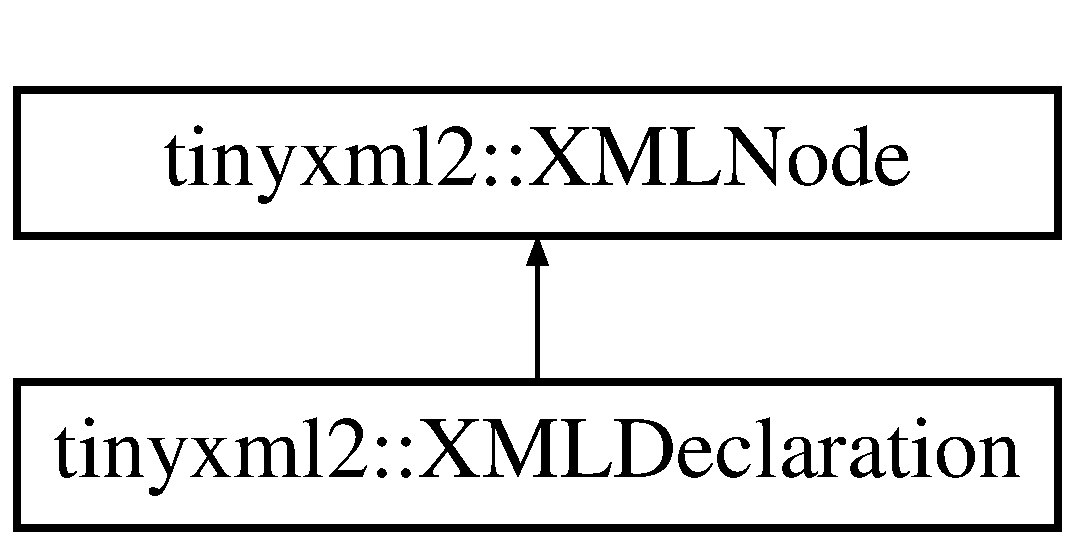
\includegraphics[height=2.000000cm]{classtinyxml2_1_1_x_m_l_declaration}
\end{center}
\end{figure}
\subsection*{Public Member Functions}
\begin{DoxyCompactItemize}
\item 
virtual \mbox{\hyperlink{classtinyxml2_1_1_x_m_l_declaration}{X\+M\+L\+Declaration}} $\ast$ \mbox{\hyperlink{classtinyxml2_1_1_x_m_l_declaration_a159d8ac45865215e88059ea1e5b52fc5}{To\+Declaration}} ()
\begin{DoxyCompactList}\small\item\em Safely cast to a Declaration, or null. \end{DoxyCompactList}\item 
virtual const \mbox{\hyperlink{classtinyxml2_1_1_x_m_l_declaration}{X\+M\+L\+Declaration}} $\ast$ \mbox{\hyperlink{classtinyxml2_1_1_x_m_l_declaration_aa20c3315b18c3b88830dccf5c493259b}{To\+Declaration}} () const
\item 
virtual bool \mbox{\hyperlink{classtinyxml2_1_1_x_m_l_declaration_acf47629d9fc08ed6f1c164a97bcf794b}{Accept}} (\mbox{\hyperlink{classtinyxml2_1_1_x_m_l_visitor}{X\+M\+L\+Visitor}} $\ast$visitor) const
\item 
virtual \mbox{\hyperlink{classtinyxml2_1_1_x_m_l_node}{X\+M\+L\+Node}} $\ast$ \mbox{\hyperlink{classtinyxml2_1_1_x_m_l_declaration_ad9d60e6d2df75c13eb6bf7319985b747}{Shallow\+Clone}} (\mbox{\hyperlink{classtinyxml2_1_1_x_m_l_document}{X\+M\+L\+Document}} $\ast$document) const
\item 
virtual bool \mbox{\hyperlink{classtinyxml2_1_1_x_m_l_declaration_ae8b4d3a399857029f36c322b0801b69c}{Shallow\+Equal}} (const \mbox{\hyperlink{classtinyxml2_1_1_x_m_l_node}{X\+M\+L\+Node}} $\ast$compare) const
\end{DoxyCompactItemize}
\subsection*{Protected Member Functions}
\begin{DoxyCompactItemize}
\item 
\mbox{\hyperlink{classtinyxml2_1_1_x_m_l_declaration_aef9586f2ce5df5feba74dde49a242b06}{X\+M\+L\+Declaration}} (\mbox{\hyperlink{classtinyxml2_1_1_x_m_l_document}{X\+M\+L\+Document}} $\ast$doc)
\item 
virtual \mbox{\hyperlink{classtinyxml2_1_1_x_m_l_declaration_ab93d5bf4f5d58b4144963cf739cf6dcc}{$\sim$\+X\+M\+L\+Declaration}} ()
\item 
char $\ast$ \mbox{\hyperlink{classtinyxml2_1_1_x_m_l_declaration_a42a2a36f4d78dc745063b79c16538b9b}{Parse\+Deep}} (char $\ast$p, \mbox{\hyperlink{classtinyxml2_1_1_str_pair}{Str\+Pair}} $\ast$parent\+End\+Tag, int $\ast$cur\+Line\+Num\+Ptr)
\end{DoxyCompactItemize}
\subsection*{Friends}
\begin{DoxyCompactItemize}
\item 
class \mbox{\hyperlink{classtinyxml2_1_1_x_m_l_declaration_a4eee3bda60c60a30e4e8cd4ea91c4c6e}{X\+M\+L\+Document}}
\end{DoxyCompactItemize}
\subsection*{Additional Inherited Members}


\subsection{Detailed Description}
In correct X\+ML the declaration is the first entry in the file. \begin{DoxyVerb}    <?xml version="1.0" standalone="yes"?>
\end{DoxyVerb}


Tiny\+X\+M\+L-\/2 will happily read or write files without a declaration, however.

The text of the declaration isn\textquotesingle{}t interpreted. It is parsed and written as a string. 

\subsection{Constructor \& Destructor Documentation}
\mbox{\Hypertarget{classtinyxml2_1_1_x_m_l_declaration_aef9586f2ce5df5feba74dde49a242b06}\label{classtinyxml2_1_1_x_m_l_declaration_aef9586f2ce5df5feba74dde49a242b06}} 
\index{tinyxml2\+::\+X\+M\+L\+Declaration@{tinyxml2\+::\+X\+M\+L\+Declaration}!X\+M\+L\+Declaration@{X\+M\+L\+Declaration}}
\index{X\+M\+L\+Declaration@{X\+M\+L\+Declaration}!tinyxml2\+::\+X\+M\+L\+Declaration@{tinyxml2\+::\+X\+M\+L\+Declaration}}
\subsubsection{\texorpdfstring{X\+M\+L\+Declaration()}{XMLDeclaration()}}
{\footnotesize\ttfamily tinyxml2\+::\+X\+M\+L\+Declaration\+::\+X\+M\+L\+Declaration (\begin{DoxyParamCaption}\item[{\mbox{\hyperlink{classtinyxml2_1_1_x_m_l_document}{X\+M\+L\+Document}} $\ast$}]{doc }\end{DoxyParamCaption})\hspace{0.3cm}{\ttfamily [protected]}}

\mbox{\Hypertarget{classtinyxml2_1_1_x_m_l_declaration_ab93d5bf4f5d58b4144963cf739cf6dcc}\label{classtinyxml2_1_1_x_m_l_declaration_ab93d5bf4f5d58b4144963cf739cf6dcc}} 
\index{tinyxml2\+::\+X\+M\+L\+Declaration@{tinyxml2\+::\+X\+M\+L\+Declaration}!````~X\+M\+L\+Declaration@{$\sim$\+X\+M\+L\+Declaration}}
\index{````~X\+M\+L\+Declaration@{$\sim$\+X\+M\+L\+Declaration}!tinyxml2\+::\+X\+M\+L\+Declaration@{tinyxml2\+::\+X\+M\+L\+Declaration}}
\subsubsection{\texorpdfstring{$\sim$\+X\+M\+L\+Declaration()}{~XMLDeclaration()}}
{\footnotesize\ttfamily tinyxml2\+::\+X\+M\+L\+Declaration\+::$\sim$\+X\+M\+L\+Declaration (\begin{DoxyParamCaption}{ }\end{DoxyParamCaption})\hspace{0.3cm}{\ttfamily [protected]}, {\ttfamily [virtual]}}



\subsection{Member Function Documentation}
\mbox{\Hypertarget{classtinyxml2_1_1_x_m_l_declaration_acf47629d9fc08ed6f1c164a97bcf794b}\label{classtinyxml2_1_1_x_m_l_declaration_acf47629d9fc08ed6f1c164a97bcf794b}} 
\index{tinyxml2\+::\+X\+M\+L\+Declaration@{tinyxml2\+::\+X\+M\+L\+Declaration}!Accept@{Accept}}
\index{Accept@{Accept}!tinyxml2\+::\+X\+M\+L\+Declaration@{tinyxml2\+::\+X\+M\+L\+Declaration}}
\subsubsection{\texorpdfstring{Accept()}{Accept()}}
{\footnotesize\ttfamily bool tinyxml2\+::\+X\+M\+L\+Declaration\+::\+Accept (\begin{DoxyParamCaption}\item[{\mbox{\hyperlink{classtinyxml2_1_1_x_m_l_visitor}{X\+M\+L\+Visitor}} $\ast$}]{visitor }\end{DoxyParamCaption}) const\hspace{0.3cm}{\ttfamily [virtual]}}

Accept a hierarchical visit of the nodes in the Tiny\+X\+M\+L-\/2 D\+OM. Every node in the X\+ML tree will be conditionally visited and the host will be called back via the \mbox{\hyperlink{classtinyxml2_1_1_x_m_l_visitor}{X\+M\+L\+Visitor}} interface.

This is essentially a S\+AX interface for Tiny\+X\+M\+L-\/2. (Note however it doesn\textquotesingle{}t re-\/parse the X\+ML for the callbacks, so the performance of Tiny\+X\+M\+L-\/2 is unchanged by using this interface versus any other.)

The interface has been based on ideas from\+:


\begin{DoxyItemize}
\item \href{http://www.saxproject.org/}{\tt http\+://www.\+saxproject.\+org/}
\item \href{http://c2.com/cgi/wiki?HierarchicalVisitorPattern}{\tt http\+://c2.\+com/cgi/wiki?\+Hierarchical\+Visitor\+Pattern}
\end{DoxyItemize}

Which are both good references for \char`\"{}visiting\char`\"{}.

An example of using \mbox{\hyperlink{classtinyxml2_1_1_x_m_l_declaration_acf47629d9fc08ed6f1c164a97bcf794b}{Accept()}}\+: \begin{DoxyVerb}XMLPrinter printer;
tinyxmlDoc.Accept( &printer );
const char* xmlcstr = printer.CStr();
\end{DoxyVerb}
 

Implements \mbox{\hyperlink{classtinyxml2_1_1_x_m_l_node_a81e66df0a44c67a7af17f3b77a152785}{tinyxml2\+::\+X\+M\+L\+Node}}.

\mbox{\Hypertarget{classtinyxml2_1_1_x_m_l_declaration_a42a2a36f4d78dc745063b79c16538b9b}\label{classtinyxml2_1_1_x_m_l_declaration_a42a2a36f4d78dc745063b79c16538b9b}} 
\index{tinyxml2\+::\+X\+M\+L\+Declaration@{tinyxml2\+::\+X\+M\+L\+Declaration}!Parse\+Deep@{Parse\+Deep}}
\index{Parse\+Deep@{Parse\+Deep}!tinyxml2\+::\+X\+M\+L\+Declaration@{tinyxml2\+::\+X\+M\+L\+Declaration}}
\subsubsection{\texorpdfstring{Parse\+Deep()}{ParseDeep()}}
{\footnotesize\ttfamily char $\ast$ tinyxml2\+::\+X\+M\+L\+Declaration\+::\+Parse\+Deep (\begin{DoxyParamCaption}\item[{char $\ast$}]{p,  }\item[{\mbox{\hyperlink{classtinyxml2_1_1_str_pair}{Str\+Pair}} $\ast$}]{parent\+End\+Tag,  }\item[{int $\ast$}]{cur\+Line\+Num\+Ptr }\end{DoxyParamCaption})\hspace{0.3cm}{\ttfamily [protected]}, {\ttfamily [virtual]}}



Reimplemented from \mbox{\hyperlink{classtinyxml2_1_1_x_m_l_node_a916e498914baecbc9a1f012352ef7c69}{tinyxml2\+::\+X\+M\+L\+Node}}.

\mbox{\Hypertarget{classtinyxml2_1_1_x_m_l_declaration_ad9d60e6d2df75c13eb6bf7319985b747}\label{classtinyxml2_1_1_x_m_l_declaration_ad9d60e6d2df75c13eb6bf7319985b747}} 
\index{tinyxml2\+::\+X\+M\+L\+Declaration@{tinyxml2\+::\+X\+M\+L\+Declaration}!Shallow\+Clone@{Shallow\+Clone}}
\index{Shallow\+Clone@{Shallow\+Clone}!tinyxml2\+::\+X\+M\+L\+Declaration@{tinyxml2\+::\+X\+M\+L\+Declaration}}
\subsubsection{\texorpdfstring{Shallow\+Clone()}{ShallowClone()}}
{\footnotesize\ttfamily \mbox{\hyperlink{classtinyxml2_1_1_x_m_l_node}{X\+M\+L\+Node}} $\ast$ tinyxml2\+::\+X\+M\+L\+Declaration\+::\+Shallow\+Clone (\begin{DoxyParamCaption}\item[{\mbox{\hyperlink{classtinyxml2_1_1_x_m_l_document}{X\+M\+L\+Document}} $\ast$}]{document }\end{DoxyParamCaption}) const\hspace{0.3cm}{\ttfamily [virtual]}}

Make a copy of this node, but not its children. You may pass in a Document pointer that will be the owner of the new Node. If the \textquotesingle{}document\textquotesingle{} is null, then the node returned will be allocated from the current Document. (this-\/$>$\mbox{\hyperlink{classtinyxml2_1_1_x_m_l_node_af343d1ef0b45c0020e62d784d7e67a68}{Get\+Document()}})

Note\+: if called on a \mbox{\hyperlink{classtinyxml2_1_1_x_m_l_document}{X\+M\+L\+Document}}, this will return null. 

Implements \mbox{\hyperlink{classtinyxml2_1_1_x_m_l_node_a8402cbd3129d20e9e6024bbcc0531283}{tinyxml2\+::\+X\+M\+L\+Node}}.

\mbox{\Hypertarget{classtinyxml2_1_1_x_m_l_declaration_ae8b4d3a399857029f36c322b0801b69c}\label{classtinyxml2_1_1_x_m_l_declaration_ae8b4d3a399857029f36c322b0801b69c}} 
\index{tinyxml2\+::\+X\+M\+L\+Declaration@{tinyxml2\+::\+X\+M\+L\+Declaration}!Shallow\+Equal@{Shallow\+Equal}}
\index{Shallow\+Equal@{Shallow\+Equal}!tinyxml2\+::\+X\+M\+L\+Declaration@{tinyxml2\+::\+X\+M\+L\+Declaration}}
\subsubsection{\texorpdfstring{Shallow\+Equal()}{ShallowEqual()}}
{\footnotesize\ttfamily bool tinyxml2\+::\+X\+M\+L\+Declaration\+::\+Shallow\+Equal (\begin{DoxyParamCaption}\item[{const \mbox{\hyperlink{classtinyxml2_1_1_x_m_l_node}{X\+M\+L\+Node}} $\ast$}]{compare }\end{DoxyParamCaption}) const\hspace{0.3cm}{\ttfamily [virtual]}}

Test if 2 nodes are the same, but don\textquotesingle{}t test children. The 2 nodes do not need to be in the same Document.

Note\+: if called on a \mbox{\hyperlink{classtinyxml2_1_1_x_m_l_document}{X\+M\+L\+Document}}, this will return false. 

Implements \mbox{\hyperlink{classtinyxml2_1_1_x_m_l_node_a7ce18b751c3ea09eac292dca264f9226}{tinyxml2\+::\+X\+M\+L\+Node}}.

\mbox{\Hypertarget{classtinyxml2_1_1_x_m_l_declaration_a159d8ac45865215e88059ea1e5b52fc5}\label{classtinyxml2_1_1_x_m_l_declaration_a159d8ac45865215e88059ea1e5b52fc5}} 
\index{tinyxml2\+::\+X\+M\+L\+Declaration@{tinyxml2\+::\+X\+M\+L\+Declaration}!To\+Declaration@{To\+Declaration}}
\index{To\+Declaration@{To\+Declaration}!tinyxml2\+::\+X\+M\+L\+Declaration@{tinyxml2\+::\+X\+M\+L\+Declaration}}
\subsubsection{\texorpdfstring{To\+Declaration()}{ToDeclaration()}\hspace{0.1cm}{\footnotesize\ttfamily [1/2]}}
{\footnotesize\ttfamily virtual \mbox{\hyperlink{classtinyxml2_1_1_x_m_l_declaration}{X\+M\+L\+Declaration}}$\ast$ tinyxml2\+::\+X\+M\+L\+Declaration\+::\+To\+Declaration (\begin{DoxyParamCaption}{ }\end{DoxyParamCaption})\hspace{0.3cm}{\ttfamily [inline]}, {\ttfamily [virtual]}}



Safely cast to a Declaration, or null. 



Reimplemented from \mbox{\hyperlink{classtinyxml2_1_1_x_m_l_node_a174fd4c22c010b58138c1b84a0dfbd51}{tinyxml2\+::\+X\+M\+L\+Node}}.

\mbox{\Hypertarget{classtinyxml2_1_1_x_m_l_declaration_aa20c3315b18c3b88830dccf5c493259b}\label{classtinyxml2_1_1_x_m_l_declaration_aa20c3315b18c3b88830dccf5c493259b}} 
\index{tinyxml2\+::\+X\+M\+L\+Declaration@{tinyxml2\+::\+X\+M\+L\+Declaration}!To\+Declaration@{To\+Declaration}}
\index{To\+Declaration@{To\+Declaration}!tinyxml2\+::\+X\+M\+L\+Declaration@{tinyxml2\+::\+X\+M\+L\+Declaration}}
\subsubsection{\texorpdfstring{To\+Declaration()}{ToDeclaration()}\hspace{0.1cm}{\footnotesize\ttfamily [2/2]}}
{\footnotesize\ttfamily virtual const \mbox{\hyperlink{classtinyxml2_1_1_x_m_l_declaration}{X\+M\+L\+Declaration}}$\ast$ tinyxml2\+::\+X\+M\+L\+Declaration\+::\+To\+Declaration (\begin{DoxyParamCaption}{ }\end{DoxyParamCaption}) const\hspace{0.3cm}{\ttfamily [inline]}, {\ttfamily [virtual]}}



Reimplemented from \mbox{\hyperlink{classtinyxml2_1_1_x_m_l_node_ac48bb4bf9eb7bb3654ad4b94945db9a1}{tinyxml2\+::\+X\+M\+L\+Node}}.



\subsection{Friends And Related Function Documentation}
\mbox{\Hypertarget{classtinyxml2_1_1_x_m_l_declaration_a4eee3bda60c60a30e4e8cd4ea91c4c6e}\label{classtinyxml2_1_1_x_m_l_declaration_a4eee3bda60c60a30e4e8cd4ea91c4c6e}} 
\index{tinyxml2\+::\+X\+M\+L\+Declaration@{tinyxml2\+::\+X\+M\+L\+Declaration}!X\+M\+L\+Document@{X\+M\+L\+Document}}
\index{X\+M\+L\+Document@{X\+M\+L\+Document}!tinyxml2\+::\+X\+M\+L\+Declaration@{tinyxml2\+::\+X\+M\+L\+Declaration}}
\subsubsection{\texorpdfstring{X\+M\+L\+Document}{XMLDocument}}
{\footnotesize\ttfamily friend class \mbox{\hyperlink{classtinyxml2_1_1_x_m_l_document}{X\+M\+L\+Document}}\hspace{0.3cm}{\ttfamily [friend]}}



The documentation for this class was generated from the following files\+:\begin{DoxyCompactItemize}
\item 
\mbox{\hyperlink{tinyxml2_8h}{tinyxml2.\+h}}\item 
\mbox{\hyperlink{tinyxml2_8cpp}{tinyxml2.\+cpp}}\end{DoxyCompactItemize}

\hypertarget{classtinyxml2_1_1_x_m_l_document}{}\section{tinyxml2\+:\+:X\+M\+L\+Document Class Reference}
\label{classtinyxml2_1_1_x_m_l_document}\index{tinyxml2\+::\+X\+M\+L\+Document@{tinyxml2\+::\+X\+M\+L\+Document}}


{\ttfamily \#include $<$tinyxml2.\+h$>$}

Inheritance diagram for tinyxml2\+:\+:X\+M\+L\+Document\+:\begin{figure}[H]
\begin{center}
\leavevmode
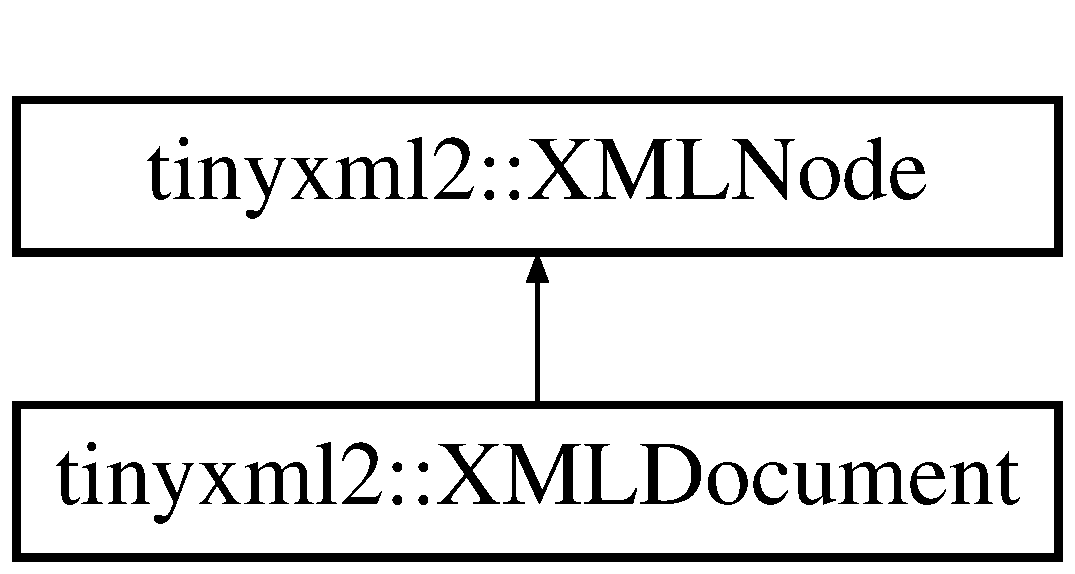
\includegraphics[height=2.000000cm]{classtinyxml2_1_1_x_m_l_document}
\end{center}
\end{figure}
\subsection*{Public Member Functions}
\begin{DoxyCompactItemize}
\item 
\mbox{\Hypertarget{classtinyxml2_1_1_x_m_l_document_a57ddf17b6e054dda10af98991b1b8f70}\label{classtinyxml2_1_1_x_m_l_document_a57ddf17b6e054dda10af98991b1b8f70}} 
\mbox{\hyperlink{classtinyxml2_1_1_x_m_l_document_a57ddf17b6e054dda10af98991b1b8f70}{X\+M\+L\+Document}} (bool process\+Entities=true, Whitespace whitespace\+Mode=P\+R\+E\+S\+E\+R\+V\+E\+\_\+\+W\+H\+I\+T\+E\+S\+P\+A\+CE)
\begin{DoxyCompactList}\small\item\em constructor \end{DoxyCompactList}\item 
\mbox{\Hypertarget{classtinyxml2_1_1_x_m_l_document_a3e185f880882bd978367bb55937735ec}\label{classtinyxml2_1_1_x_m_l_document_a3e185f880882bd978367bb55937735ec}} 
virtual \mbox{\hyperlink{classtinyxml2_1_1_x_m_l_document}{X\+M\+L\+Document}} $\ast$ \mbox{\hyperlink{classtinyxml2_1_1_x_m_l_document_a3e185f880882bd978367bb55937735ec}{To\+Document}} ()
\begin{DoxyCompactList}\small\item\em Safely cast to a Document, or null. \end{DoxyCompactList}\item 
\mbox{\Hypertarget{classtinyxml2_1_1_x_m_l_document_a747ab173887d969fe313b4617f968e99}\label{classtinyxml2_1_1_x_m_l_document_a747ab173887d969fe313b4617f968e99}} 
virtual const \mbox{\hyperlink{classtinyxml2_1_1_x_m_l_document}{X\+M\+L\+Document}} $\ast$ {\bfseries To\+Document} () const
\item 
X\+M\+L\+Error \mbox{\hyperlink{classtinyxml2_1_1_x_m_l_document_a1819bd34f540a7304c105a6232d25a1f}{Parse}} (const char $\ast$xml, size\+\_\+t n\+Bytes=(size\+\_\+t)(-\/1))
\item 
X\+M\+L\+Error \mbox{\hyperlink{classtinyxml2_1_1_x_m_l_document_a2ebd4647a8af5fc6831b294ac26a150a}{Load\+File}} (const char $\ast$filename)
\item 
X\+M\+L\+Error \mbox{\hyperlink{classtinyxml2_1_1_x_m_l_document_a5f1d330fad44c52f3d265338dd2a6dc2}{Load\+File}} (F\+I\+LE $\ast$)
\item 
X\+M\+L\+Error \mbox{\hyperlink{classtinyxml2_1_1_x_m_l_document_a73ac416b4a2aa0952e841220eb3da18f}{Save\+File}} (const char $\ast$filename, bool compact=false)
\item 
X\+M\+L\+Error \mbox{\hyperlink{classtinyxml2_1_1_x_m_l_document_a8b95779479a0035acc67b3a61dfe1b74}{Save\+File}} (F\+I\+LE $\ast$fp, bool compact=false)
\item 
\mbox{\Hypertarget{classtinyxml2_1_1_x_m_l_document_a53e6c035b1b539563fef8c817fb30469}\label{classtinyxml2_1_1_x_m_l_document_a53e6c035b1b539563fef8c817fb30469}} 
bool {\bfseries Process\+Entities} () const
\item 
\mbox{\Hypertarget{classtinyxml2_1_1_x_m_l_document_a810ce508e6e0365497c2a9deb83c9ca7}\label{classtinyxml2_1_1_x_m_l_document_a810ce508e6e0365497c2a9deb83c9ca7}} 
Whitespace {\bfseries Whitespace\+Mode} () const
\item 
bool \mbox{\hyperlink{classtinyxml2_1_1_x_m_l_document_a33fc5d159db873a179fa26338adb05bd}{Has\+B\+OM}} () const
\item 
void \mbox{\hyperlink{classtinyxml2_1_1_x_m_l_document_a14419b698f7c4b140df4e80f3f0c93b0}{Set\+B\+OM}} (bool use\+B\+OM)
\item 
\mbox{\hyperlink{classtinyxml2_1_1_x_m_l_element}{X\+M\+L\+Element}} $\ast$ \mbox{\hyperlink{classtinyxml2_1_1_x_m_l_document_ad2b70320d3c2a071c2f36928edff3e1c}{Root\+Element}} ()
\item 
\mbox{\Hypertarget{classtinyxml2_1_1_x_m_l_document_a2be8ef9d6346bdef34311f91529afae4}\label{classtinyxml2_1_1_x_m_l_document_a2be8ef9d6346bdef34311f91529afae4}} 
const \mbox{\hyperlink{classtinyxml2_1_1_x_m_l_element}{X\+M\+L\+Element}} $\ast$ {\bfseries Root\+Element} () const
\item 
void \mbox{\hyperlink{classtinyxml2_1_1_x_m_l_document_a867cf5fa3e3ff6ae4847a8b7ee8ec083}{Print}} (\mbox{\hyperlink{classtinyxml2_1_1_x_m_l_printer}{X\+M\+L\+Printer}} $\ast$streamer=0) const
\item 
virtual bool \mbox{\hyperlink{classtinyxml2_1_1_x_m_l_document_ab7be651917a35ab1ff0e4e6d4e565cdf}{Accept}} (\mbox{\hyperlink{classtinyxml2_1_1_x_m_l_visitor}{X\+M\+L\+Visitor}} $\ast$visitor) const
\item 
\mbox{\hyperlink{classtinyxml2_1_1_x_m_l_element}{X\+M\+L\+Element}} $\ast$ \mbox{\hyperlink{classtinyxml2_1_1_x_m_l_document_a3c335a700a43d7c363a393142a23f234}{New\+Element}} (const char $\ast$name)
\item 
\mbox{\hyperlink{classtinyxml2_1_1_x_m_l_comment}{X\+M\+L\+Comment}} $\ast$ \mbox{\hyperlink{classtinyxml2_1_1_x_m_l_document_a386df0befd06aadb5e0cd21381aa955a}{New\+Comment}} (const char $\ast$comment)
\item 
\mbox{\hyperlink{classtinyxml2_1_1_x_m_l_text}{X\+M\+L\+Text}} $\ast$ \mbox{\hyperlink{classtinyxml2_1_1_x_m_l_document_acece5de77a0819f2341b08c1e1ed9987}{New\+Text}} (const char $\ast$text)
\item 
\mbox{\hyperlink{classtinyxml2_1_1_x_m_l_declaration}{X\+M\+L\+Declaration}} $\ast$ \mbox{\hyperlink{classtinyxml2_1_1_x_m_l_document_ae519030c0262fa2daff8993681990e16}{New\+Declaration}} (const char $\ast$text=0)
\item 
\mbox{\hyperlink{classtinyxml2_1_1_x_m_l_unknown}{X\+M\+L\+Unknown}} $\ast$ \mbox{\hyperlink{classtinyxml2_1_1_x_m_l_document_a4954f502c5fd7f49de54c3c0c99bb73d}{New\+Unknown}} (const char $\ast$text)
\item 
void \mbox{\hyperlink{classtinyxml2_1_1_x_m_l_document_ac1d6e2c7fcc1a660624ac4f68e96380d}{Delete\+Node}} (\mbox{\hyperlink{classtinyxml2_1_1_x_m_l_node}{X\+M\+L\+Node}} $\ast$node)
\item 
\mbox{\Hypertarget{classtinyxml2_1_1_x_m_l_document_a4085d9c52f1d93214311459d6d1fcf17}\label{classtinyxml2_1_1_x_m_l_document_a4085d9c52f1d93214311459d6d1fcf17}} 
void {\bfseries Clear\+Error} ()
\item 
\mbox{\Hypertarget{classtinyxml2_1_1_x_m_l_document_a34e6318e182e40e3cc4f4ba5d59ed9ed}\label{classtinyxml2_1_1_x_m_l_document_a34e6318e182e40e3cc4f4ba5d59ed9ed}} 
bool \mbox{\hyperlink{classtinyxml2_1_1_x_m_l_document_a34e6318e182e40e3cc4f4ba5d59ed9ed}{Error}} () const
\begin{DoxyCompactList}\small\item\em Return true if there was an error parsing the document. \end{DoxyCompactList}\item 
\mbox{\Hypertarget{classtinyxml2_1_1_x_m_l_document_afa3ed33b3107f920ec2b301f805ac17d}\label{classtinyxml2_1_1_x_m_l_document_afa3ed33b3107f920ec2b301f805ac17d}} 
X\+M\+L\+Error \mbox{\hyperlink{classtinyxml2_1_1_x_m_l_document_afa3ed33b3107f920ec2b301f805ac17d}{Error\+ID}} () const
\begin{DoxyCompactList}\small\item\em Return the error\+ID. \end{DoxyCompactList}\item 
\mbox{\Hypertarget{classtinyxml2_1_1_x_m_l_document_a1a5f2b63427caffd4cde15781d9d11f9}\label{classtinyxml2_1_1_x_m_l_document_a1a5f2b63427caffd4cde15781d9d11f9}} 
const char $\ast$ {\bfseries Error\+Name} () const
\item 
const char $\ast$ \mbox{\hyperlink{classtinyxml2_1_1_x_m_l_document_ae97fff2402a0d01e0509c430b37996b3}{Error\+Str}} () const
\item 
\mbox{\Hypertarget{classtinyxml2_1_1_x_m_l_document_a1d033945b42e125d933d6231e4571552}\label{classtinyxml2_1_1_x_m_l_document_a1d033945b42e125d933d6231e4571552}} 
void \mbox{\hyperlink{classtinyxml2_1_1_x_m_l_document_a1d033945b42e125d933d6231e4571552}{Print\+Error}} () const
\begin{DoxyCompactList}\small\item\em A (trivial) utility function that prints the \mbox{\hyperlink{classtinyxml2_1_1_x_m_l_document_ae97fff2402a0d01e0509c430b37996b3}{Error\+Str()}} to stdout. \end{DoxyCompactList}\item 
\mbox{\Hypertarget{classtinyxml2_1_1_x_m_l_document_a57400f816dbe7799ece33615ead9ab76}\label{classtinyxml2_1_1_x_m_l_document_a57400f816dbe7799ece33615ead9ab76}} 
int \mbox{\hyperlink{classtinyxml2_1_1_x_m_l_document_a57400f816dbe7799ece33615ead9ab76}{Error\+Line\+Num}} () const
\begin{DoxyCompactList}\small\item\em Return the line where the error occurred, or zero if unknown. \end{DoxyCompactList}\item 
\mbox{\Hypertarget{classtinyxml2_1_1_x_m_l_document_a65656b0b2cbc822708eb351504178aaf}\label{classtinyxml2_1_1_x_m_l_document_a65656b0b2cbc822708eb351504178aaf}} 
void \mbox{\hyperlink{classtinyxml2_1_1_x_m_l_document_a65656b0b2cbc822708eb351504178aaf}{Clear}} ()
\begin{DoxyCompactList}\small\item\em Clear the document, resetting it to the initial state. \end{DoxyCompactList}\item 
void \mbox{\hyperlink{classtinyxml2_1_1_x_m_l_document_af592ffc91514e25a39664521ac83db45}{Deep\+Copy}} (\mbox{\hyperlink{classtinyxml2_1_1_x_m_l_document}{X\+M\+L\+Document}} $\ast$target) const
\item 
\mbox{\Hypertarget{classtinyxml2_1_1_x_m_l_document_a25827d1bec509ad566a107e5853ed040}\label{classtinyxml2_1_1_x_m_l_document_a25827d1bec509ad566a107e5853ed040}} 
char $\ast$ {\bfseries Identify} (char $\ast$p, \mbox{\hyperlink{classtinyxml2_1_1_x_m_l_node}{X\+M\+L\+Node}} $\ast$$\ast$node)
\item 
\mbox{\Hypertarget{classtinyxml2_1_1_x_m_l_document_a95d28ecb4760a994556b0a51690b21be}\label{classtinyxml2_1_1_x_m_l_document_a95d28ecb4760a994556b0a51690b21be}} 
void {\bfseries Mark\+In\+Use} (\mbox{\hyperlink{classtinyxml2_1_1_x_m_l_node}{X\+M\+L\+Node}} $\ast$)
\item 
virtual \mbox{\hyperlink{classtinyxml2_1_1_x_m_l_node}{X\+M\+L\+Node}} $\ast$ \mbox{\hyperlink{classtinyxml2_1_1_x_m_l_document_aa37cc1709d7e1e988bc17dcfb24a69b8}{Shallow\+Clone}} (\mbox{\hyperlink{classtinyxml2_1_1_x_m_l_document}{X\+M\+L\+Document}} $\ast$) const
\item 
virtual bool \mbox{\hyperlink{classtinyxml2_1_1_x_m_l_document_a6fe5ef18699091844fcf64b56ffa5bf9}{Shallow\+Equal}} (const \mbox{\hyperlink{classtinyxml2_1_1_x_m_l_node}{X\+M\+L\+Node}} $\ast$) const
\end{DoxyCompactItemize}
\subsection*{Static Public Member Functions}
\begin{DoxyCompactItemize}
\item 
\mbox{\Hypertarget{classtinyxml2_1_1_x_m_l_document_a639f7c295c38dc5a4aafeb2fff93da03}\label{classtinyxml2_1_1_x_m_l_document_a639f7c295c38dc5a4aafeb2fff93da03}} 
static const char $\ast$ {\bfseries Error\+I\+D\+To\+Name} (X\+M\+L\+Error error\+ID)
\end{DoxyCompactItemize}
\subsection*{Friends}
\begin{DoxyCompactItemize}
\item 
\mbox{\Hypertarget{classtinyxml2_1_1_x_m_l_document_ac2fba9b6e452829dd892f7392c24e0eb}\label{classtinyxml2_1_1_x_m_l_document_ac2fba9b6e452829dd892f7392c24e0eb}} 
class {\bfseries X\+M\+L\+Element}
\item 
\mbox{\Hypertarget{classtinyxml2_1_1_x_m_l_document_a8233f9dc4d61d90e93be2a3647c6d957}\label{classtinyxml2_1_1_x_m_l_document_a8233f9dc4d61d90e93be2a3647c6d957}} 
class {\bfseries X\+M\+L\+Node}
\item 
\mbox{\Hypertarget{classtinyxml2_1_1_x_m_l_document_ae50b59416e98bbe7e4bc87df40092109}\label{classtinyxml2_1_1_x_m_l_document_ae50b59416e98bbe7e4bc87df40092109}} 
class {\bfseries X\+M\+L\+Text}
\item 
\mbox{\Hypertarget{classtinyxml2_1_1_x_m_l_document_acee9e261162d4236fb2c30312c54cd4c}\label{classtinyxml2_1_1_x_m_l_document_acee9e261162d4236fb2c30312c54cd4c}} 
class {\bfseries X\+M\+L\+Comment}
\item 
\mbox{\Hypertarget{classtinyxml2_1_1_x_m_l_document_a93d2c2c2db3973083b7d6e7f6f358160}\label{classtinyxml2_1_1_x_m_l_document_a93d2c2c2db3973083b7d6e7f6f358160}} 
class {\bfseries X\+M\+L\+Declaration}
\item 
\mbox{\Hypertarget{classtinyxml2_1_1_x_m_l_document_a6946948274f7a02f5e69b5dbeaea9b35}\label{classtinyxml2_1_1_x_m_l_document_a6946948274f7a02f5e69b5dbeaea9b35}} 
class {\bfseries X\+M\+L\+Unknown}
\end{DoxyCompactItemize}
\subsection*{Additional Inherited Members}


\subsection{Detailed Description}
A Document binds together all the functionality. It can be saved, loaded, and printed to the screen. All Nodes are connected and allocated to a Document. If the Document is deleted, all its Nodes are also deleted. 

\subsection{Member Function Documentation}
\mbox{\Hypertarget{classtinyxml2_1_1_x_m_l_document_ab7be651917a35ab1ff0e4e6d4e565cdf}\label{classtinyxml2_1_1_x_m_l_document_ab7be651917a35ab1ff0e4e6d4e565cdf}} 
\index{tinyxml2\+::\+X\+M\+L\+Document@{tinyxml2\+::\+X\+M\+L\+Document}!Accept@{Accept}}
\index{Accept@{Accept}!tinyxml2\+::\+X\+M\+L\+Document@{tinyxml2\+::\+X\+M\+L\+Document}}
\subsubsection{\texorpdfstring{Accept()}{Accept()}}
{\footnotesize\ttfamily bool tinyxml2\+::\+X\+M\+L\+Document\+::\+Accept (\begin{DoxyParamCaption}\item[{\mbox{\hyperlink{classtinyxml2_1_1_x_m_l_visitor}{X\+M\+L\+Visitor}} $\ast$}]{visitor }\end{DoxyParamCaption}) const\hspace{0.3cm}{\ttfamily [virtual]}}

Accept a hierarchical visit of the nodes in the Tiny\+X\+M\+L-\/2 D\+OM. Every node in the X\+ML tree will be conditionally visited and the host will be called back via the \mbox{\hyperlink{classtinyxml2_1_1_x_m_l_visitor}{X\+M\+L\+Visitor}} interface.

This is essentially a S\+AX interface for Tiny\+X\+M\+L-\/2. (Note however it doesn\textquotesingle{}t re-\/parse the X\+ML for the callbacks, so the performance of Tiny\+X\+M\+L-\/2 is unchanged by using this interface versus any other.)

The interface has been based on ideas from\+:


\begin{DoxyItemize}
\item \href{http://www.saxproject.org/}{\tt http\+://www.\+saxproject.\+org/}
\item \href{http://c2.com/cgi/wiki?HierarchicalVisitorPattern}{\tt http\+://c2.\+com/cgi/wiki?\+Hierarchical\+Visitor\+Pattern}
\end{DoxyItemize}

Which are both good references for \char`\"{}visiting\char`\"{}.

An example of using \mbox{\hyperlink{classtinyxml2_1_1_x_m_l_document_ab7be651917a35ab1ff0e4e6d4e565cdf}{Accept()}}\+: \begin{DoxyVerb}XMLPrinter printer;
tinyxmlDoc.Accept( &printer );
const char* xmlcstr = printer.CStr();
\end{DoxyVerb}
 

Implements \mbox{\hyperlink{classtinyxml2_1_1_x_m_l_node_a81e66df0a44c67a7af17f3b77a152785}{tinyxml2\+::\+X\+M\+L\+Node}}.

\mbox{\Hypertarget{classtinyxml2_1_1_x_m_l_document_af592ffc91514e25a39664521ac83db45}\label{classtinyxml2_1_1_x_m_l_document_af592ffc91514e25a39664521ac83db45}} 
\index{tinyxml2\+::\+X\+M\+L\+Document@{tinyxml2\+::\+X\+M\+L\+Document}!Deep\+Copy@{Deep\+Copy}}
\index{Deep\+Copy@{Deep\+Copy}!tinyxml2\+::\+X\+M\+L\+Document@{tinyxml2\+::\+X\+M\+L\+Document}}
\subsubsection{\texorpdfstring{Deep\+Copy()}{DeepCopy()}}
{\footnotesize\ttfamily void tinyxml2\+::\+X\+M\+L\+Document\+::\+Deep\+Copy (\begin{DoxyParamCaption}\item[{\mbox{\hyperlink{classtinyxml2_1_1_x_m_l_document}{X\+M\+L\+Document}} $\ast$}]{target }\end{DoxyParamCaption}) const}

Copies this document to a target document. The target will be completely cleared before the copy. If you want to copy a sub-\/tree, see \mbox{\hyperlink{classtinyxml2_1_1_x_m_l_node_a3bb369fd733f1989b751d99a9417adab}{X\+M\+L\+Node\+::\+Deep\+Clone()}}.

N\+O\+TE\+: that the \textquotesingle{}target\textquotesingle{} must be non-\/null. \mbox{\Hypertarget{classtinyxml2_1_1_x_m_l_document_ac1d6e2c7fcc1a660624ac4f68e96380d}\label{classtinyxml2_1_1_x_m_l_document_ac1d6e2c7fcc1a660624ac4f68e96380d}} 
\index{tinyxml2\+::\+X\+M\+L\+Document@{tinyxml2\+::\+X\+M\+L\+Document}!Delete\+Node@{Delete\+Node}}
\index{Delete\+Node@{Delete\+Node}!tinyxml2\+::\+X\+M\+L\+Document@{tinyxml2\+::\+X\+M\+L\+Document}}
\subsubsection{\texorpdfstring{Delete\+Node()}{DeleteNode()}}
{\footnotesize\ttfamily void tinyxml2\+::\+X\+M\+L\+Document\+::\+Delete\+Node (\begin{DoxyParamCaption}\item[{\mbox{\hyperlink{classtinyxml2_1_1_x_m_l_node}{X\+M\+L\+Node}} $\ast$}]{node }\end{DoxyParamCaption})}

Delete a node associated with this document. It will be unlinked from the D\+OM. \mbox{\Hypertarget{classtinyxml2_1_1_x_m_l_document_ae97fff2402a0d01e0509c430b37996b3}\label{classtinyxml2_1_1_x_m_l_document_ae97fff2402a0d01e0509c430b37996b3}} 
\index{tinyxml2\+::\+X\+M\+L\+Document@{tinyxml2\+::\+X\+M\+L\+Document}!Error\+Str@{Error\+Str}}
\index{Error\+Str@{Error\+Str}!tinyxml2\+::\+X\+M\+L\+Document@{tinyxml2\+::\+X\+M\+L\+Document}}
\subsubsection{\texorpdfstring{Error\+Str()}{ErrorStr()}}
{\footnotesize\ttfamily const char $\ast$ tinyxml2\+::\+X\+M\+L\+Document\+::\+Error\+Str (\begin{DoxyParamCaption}{ }\end{DoxyParamCaption}) const}

Returns a \char`\"{}long form\char`\"{} error description. A hopefully helpful diagnostic with location, line number, and/or additional info. \mbox{\Hypertarget{classtinyxml2_1_1_x_m_l_document_a33fc5d159db873a179fa26338adb05bd}\label{classtinyxml2_1_1_x_m_l_document_a33fc5d159db873a179fa26338adb05bd}} 
\index{tinyxml2\+::\+X\+M\+L\+Document@{tinyxml2\+::\+X\+M\+L\+Document}!Has\+B\+OM@{Has\+B\+OM}}
\index{Has\+B\+OM@{Has\+B\+OM}!tinyxml2\+::\+X\+M\+L\+Document@{tinyxml2\+::\+X\+M\+L\+Document}}
\subsubsection{\texorpdfstring{Has\+B\+O\+M()}{HasBOM()}}
{\footnotesize\ttfamily bool tinyxml2\+::\+X\+M\+L\+Document\+::\+Has\+B\+OM (\begin{DoxyParamCaption}{ }\end{DoxyParamCaption}) const\hspace{0.3cm}{\ttfamily [inline]}}

Returns true if this document has a leading Byte Order Mark of U\+T\+F8. \mbox{\Hypertarget{classtinyxml2_1_1_x_m_l_document_a2ebd4647a8af5fc6831b294ac26a150a}\label{classtinyxml2_1_1_x_m_l_document_a2ebd4647a8af5fc6831b294ac26a150a}} 
\index{tinyxml2\+::\+X\+M\+L\+Document@{tinyxml2\+::\+X\+M\+L\+Document}!Load\+File@{Load\+File}}
\index{Load\+File@{Load\+File}!tinyxml2\+::\+X\+M\+L\+Document@{tinyxml2\+::\+X\+M\+L\+Document}}
\subsubsection{\texorpdfstring{Load\+File()}{LoadFile()}\hspace{0.1cm}{\footnotesize\ttfamily [1/2]}}
{\footnotesize\ttfamily X\+M\+L\+Error tinyxml2\+::\+X\+M\+L\+Document\+::\+Load\+File (\begin{DoxyParamCaption}\item[{const char $\ast$}]{filename }\end{DoxyParamCaption})}

Load an X\+ML file from disk. Returns X\+M\+L\+\_\+\+S\+U\+C\+C\+E\+SS (0) on success, or an error\+ID. \mbox{\Hypertarget{classtinyxml2_1_1_x_m_l_document_a5f1d330fad44c52f3d265338dd2a6dc2}\label{classtinyxml2_1_1_x_m_l_document_a5f1d330fad44c52f3d265338dd2a6dc2}} 
\index{tinyxml2\+::\+X\+M\+L\+Document@{tinyxml2\+::\+X\+M\+L\+Document}!Load\+File@{Load\+File}}
\index{Load\+File@{Load\+File}!tinyxml2\+::\+X\+M\+L\+Document@{tinyxml2\+::\+X\+M\+L\+Document}}
\subsubsection{\texorpdfstring{Load\+File()}{LoadFile()}\hspace{0.1cm}{\footnotesize\ttfamily [2/2]}}
{\footnotesize\ttfamily X\+M\+L\+Error tinyxml2\+::\+X\+M\+L\+Document\+::\+Load\+File (\begin{DoxyParamCaption}\item[{F\+I\+LE $\ast$}]{fp }\end{DoxyParamCaption})}

Load an X\+ML file from disk. You are responsible for providing and closing the F\+I\+L\+E$\ast$.

N\+O\+TE\+: The file should be opened as binary (\char`\"{}rb\char`\"{}) not text in order for Tiny\+X\+M\+L-\/2 to correctly do newline normalization.

Returns X\+M\+L\+\_\+\+S\+U\+C\+C\+E\+SS (0) on success, or an error\+ID. \mbox{\Hypertarget{classtinyxml2_1_1_x_m_l_document_a386df0befd06aadb5e0cd21381aa955a}\label{classtinyxml2_1_1_x_m_l_document_a386df0befd06aadb5e0cd21381aa955a}} 
\index{tinyxml2\+::\+X\+M\+L\+Document@{tinyxml2\+::\+X\+M\+L\+Document}!New\+Comment@{New\+Comment}}
\index{New\+Comment@{New\+Comment}!tinyxml2\+::\+X\+M\+L\+Document@{tinyxml2\+::\+X\+M\+L\+Document}}
\subsubsection{\texorpdfstring{New\+Comment()}{NewComment()}}
{\footnotesize\ttfamily \mbox{\hyperlink{classtinyxml2_1_1_x_m_l_comment}{X\+M\+L\+Comment}} $\ast$ tinyxml2\+::\+X\+M\+L\+Document\+::\+New\+Comment (\begin{DoxyParamCaption}\item[{const char $\ast$}]{comment }\end{DoxyParamCaption})}

Create a new Comment associated with this Document. The memory for the Comment is managed by the Document. \mbox{\Hypertarget{classtinyxml2_1_1_x_m_l_document_ae519030c0262fa2daff8993681990e16}\label{classtinyxml2_1_1_x_m_l_document_ae519030c0262fa2daff8993681990e16}} 
\index{tinyxml2\+::\+X\+M\+L\+Document@{tinyxml2\+::\+X\+M\+L\+Document}!New\+Declaration@{New\+Declaration}}
\index{New\+Declaration@{New\+Declaration}!tinyxml2\+::\+X\+M\+L\+Document@{tinyxml2\+::\+X\+M\+L\+Document}}
\subsubsection{\texorpdfstring{New\+Declaration()}{NewDeclaration()}}
{\footnotesize\ttfamily \mbox{\hyperlink{classtinyxml2_1_1_x_m_l_declaration}{X\+M\+L\+Declaration}} $\ast$ tinyxml2\+::\+X\+M\+L\+Document\+::\+New\+Declaration (\begin{DoxyParamCaption}\item[{const char $\ast$}]{text = {\ttfamily 0} }\end{DoxyParamCaption})}

Create a new Declaration associated with this Document. The memory for the object is managed by the Document.

If the \textquotesingle{}text\textquotesingle{} param is null, the standard declaration is used.\+: \begin{DoxyVerb}    <?xml version="1.0" encoding="UTF-8"?>
\end{DoxyVerb}
 \mbox{\Hypertarget{classtinyxml2_1_1_x_m_l_document_a3c335a700a43d7c363a393142a23f234}\label{classtinyxml2_1_1_x_m_l_document_a3c335a700a43d7c363a393142a23f234}} 
\index{tinyxml2\+::\+X\+M\+L\+Document@{tinyxml2\+::\+X\+M\+L\+Document}!New\+Element@{New\+Element}}
\index{New\+Element@{New\+Element}!tinyxml2\+::\+X\+M\+L\+Document@{tinyxml2\+::\+X\+M\+L\+Document}}
\subsubsection{\texorpdfstring{New\+Element()}{NewElement()}}
{\footnotesize\ttfamily \mbox{\hyperlink{classtinyxml2_1_1_x_m_l_element}{X\+M\+L\+Element}} $\ast$ tinyxml2\+::\+X\+M\+L\+Document\+::\+New\+Element (\begin{DoxyParamCaption}\item[{const char $\ast$}]{name }\end{DoxyParamCaption})}

Create a new Element associated with this Document. The memory for the Element is managed by the Document. \mbox{\Hypertarget{classtinyxml2_1_1_x_m_l_document_acece5de77a0819f2341b08c1e1ed9987}\label{classtinyxml2_1_1_x_m_l_document_acece5de77a0819f2341b08c1e1ed9987}} 
\index{tinyxml2\+::\+X\+M\+L\+Document@{tinyxml2\+::\+X\+M\+L\+Document}!New\+Text@{New\+Text}}
\index{New\+Text@{New\+Text}!tinyxml2\+::\+X\+M\+L\+Document@{tinyxml2\+::\+X\+M\+L\+Document}}
\subsubsection{\texorpdfstring{New\+Text()}{NewText()}}
{\footnotesize\ttfamily \mbox{\hyperlink{classtinyxml2_1_1_x_m_l_text}{X\+M\+L\+Text}} $\ast$ tinyxml2\+::\+X\+M\+L\+Document\+::\+New\+Text (\begin{DoxyParamCaption}\item[{const char $\ast$}]{text }\end{DoxyParamCaption})}

Create a new Text associated with this Document. The memory for the Text is managed by the Document. \mbox{\Hypertarget{classtinyxml2_1_1_x_m_l_document_a4954f502c5fd7f49de54c3c0c99bb73d}\label{classtinyxml2_1_1_x_m_l_document_a4954f502c5fd7f49de54c3c0c99bb73d}} 
\index{tinyxml2\+::\+X\+M\+L\+Document@{tinyxml2\+::\+X\+M\+L\+Document}!New\+Unknown@{New\+Unknown}}
\index{New\+Unknown@{New\+Unknown}!tinyxml2\+::\+X\+M\+L\+Document@{tinyxml2\+::\+X\+M\+L\+Document}}
\subsubsection{\texorpdfstring{New\+Unknown()}{NewUnknown()}}
{\footnotesize\ttfamily \mbox{\hyperlink{classtinyxml2_1_1_x_m_l_unknown}{X\+M\+L\+Unknown}} $\ast$ tinyxml2\+::\+X\+M\+L\+Document\+::\+New\+Unknown (\begin{DoxyParamCaption}\item[{const char $\ast$}]{text }\end{DoxyParamCaption})}

Create a new Unknown associated with this Document. The memory for the object is managed by the Document. \mbox{\Hypertarget{classtinyxml2_1_1_x_m_l_document_a1819bd34f540a7304c105a6232d25a1f}\label{classtinyxml2_1_1_x_m_l_document_a1819bd34f540a7304c105a6232d25a1f}} 
\index{tinyxml2\+::\+X\+M\+L\+Document@{tinyxml2\+::\+X\+M\+L\+Document}!Parse@{Parse}}
\index{Parse@{Parse}!tinyxml2\+::\+X\+M\+L\+Document@{tinyxml2\+::\+X\+M\+L\+Document}}
\subsubsection{\texorpdfstring{Parse()}{Parse()}}
{\footnotesize\ttfamily X\+M\+L\+Error tinyxml2\+::\+X\+M\+L\+Document\+::\+Parse (\begin{DoxyParamCaption}\item[{const char $\ast$}]{xml,  }\item[{size\+\_\+t}]{n\+Bytes = {\ttfamily (size\+\_\+t)(-\/1)} }\end{DoxyParamCaption})}

Parse an X\+ML file from a character string. Returns X\+M\+L\+\_\+\+S\+U\+C\+C\+E\+SS (0) on success, or an error\+ID.

You may optionally pass in the \textquotesingle{}n\+Bytes\textquotesingle{}, which is the number of bytes which will be parsed. If not specified, Tiny\+X\+M\+L-\/2 will assume \textquotesingle{}xml\textquotesingle{} points to a null terminated string. \mbox{\Hypertarget{classtinyxml2_1_1_x_m_l_document_a867cf5fa3e3ff6ae4847a8b7ee8ec083}\label{classtinyxml2_1_1_x_m_l_document_a867cf5fa3e3ff6ae4847a8b7ee8ec083}} 
\index{tinyxml2\+::\+X\+M\+L\+Document@{tinyxml2\+::\+X\+M\+L\+Document}!Print@{Print}}
\index{Print@{Print}!tinyxml2\+::\+X\+M\+L\+Document@{tinyxml2\+::\+X\+M\+L\+Document}}
\subsubsection{\texorpdfstring{Print()}{Print()}}
{\footnotesize\ttfamily void tinyxml2\+::\+X\+M\+L\+Document\+::\+Print (\begin{DoxyParamCaption}\item[{\mbox{\hyperlink{classtinyxml2_1_1_x_m_l_printer}{X\+M\+L\+Printer}} $\ast$}]{streamer = {\ttfamily 0} }\end{DoxyParamCaption}) const}

Print the Document. If the Printer is not provided, it will print to stdout. If you provide Printer, this can print to a file\+: \begin{DoxyVerb}XMLPrinter printer( fp );
doc.Print( &printer );
\end{DoxyVerb}


Or you can use a printer to print to memory\+: \begin{DoxyVerb}XMLPrinter printer;
doc.Print( &printer );
// printer.CStr() has a const char* to the XML
\end{DoxyVerb}
 \mbox{\Hypertarget{classtinyxml2_1_1_x_m_l_document_ad2b70320d3c2a071c2f36928edff3e1c}\label{classtinyxml2_1_1_x_m_l_document_ad2b70320d3c2a071c2f36928edff3e1c}} 
\index{tinyxml2\+::\+X\+M\+L\+Document@{tinyxml2\+::\+X\+M\+L\+Document}!Root\+Element@{Root\+Element}}
\index{Root\+Element@{Root\+Element}!tinyxml2\+::\+X\+M\+L\+Document@{tinyxml2\+::\+X\+M\+L\+Document}}
\subsubsection{\texorpdfstring{Root\+Element()}{RootElement()}}
{\footnotesize\ttfamily \mbox{\hyperlink{classtinyxml2_1_1_x_m_l_element}{X\+M\+L\+Element}}$\ast$ tinyxml2\+::\+X\+M\+L\+Document\+::\+Root\+Element (\begin{DoxyParamCaption}{ }\end{DoxyParamCaption})\hspace{0.3cm}{\ttfamily [inline]}}

Return the root element of D\+OM. Equivalent to \mbox{\hyperlink{classtinyxml2_1_1_x_m_l_node_a1bec132dcf085284e0a10755f2cf0d57}{First\+Child\+Element()}}. To get the first node, use First\+Child(). \mbox{\Hypertarget{classtinyxml2_1_1_x_m_l_document_a73ac416b4a2aa0952e841220eb3da18f}\label{classtinyxml2_1_1_x_m_l_document_a73ac416b4a2aa0952e841220eb3da18f}} 
\index{tinyxml2\+::\+X\+M\+L\+Document@{tinyxml2\+::\+X\+M\+L\+Document}!Save\+File@{Save\+File}}
\index{Save\+File@{Save\+File}!tinyxml2\+::\+X\+M\+L\+Document@{tinyxml2\+::\+X\+M\+L\+Document}}
\subsubsection{\texorpdfstring{Save\+File()}{SaveFile()}\hspace{0.1cm}{\footnotesize\ttfamily [1/2]}}
{\footnotesize\ttfamily X\+M\+L\+Error tinyxml2\+::\+X\+M\+L\+Document\+::\+Save\+File (\begin{DoxyParamCaption}\item[{const char $\ast$}]{filename,  }\item[{bool}]{compact = {\ttfamily false} }\end{DoxyParamCaption})}

Save the X\+ML file to disk. Returns X\+M\+L\+\_\+\+S\+U\+C\+C\+E\+SS (0) on success, or an error\+ID. \mbox{\Hypertarget{classtinyxml2_1_1_x_m_l_document_a8b95779479a0035acc67b3a61dfe1b74}\label{classtinyxml2_1_1_x_m_l_document_a8b95779479a0035acc67b3a61dfe1b74}} 
\index{tinyxml2\+::\+X\+M\+L\+Document@{tinyxml2\+::\+X\+M\+L\+Document}!Save\+File@{Save\+File}}
\index{Save\+File@{Save\+File}!tinyxml2\+::\+X\+M\+L\+Document@{tinyxml2\+::\+X\+M\+L\+Document}}
\subsubsection{\texorpdfstring{Save\+File()}{SaveFile()}\hspace{0.1cm}{\footnotesize\ttfamily [2/2]}}
{\footnotesize\ttfamily X\+M\+L\+Error tinyxml2\+::\+X\+M\+L\+Document\+::\+Save\+File (\begin{DoxyParamCaption}\item[{F\+I\+LE $\ast$}]{fp,  }\item[{bool}]{compact = {\ttfamily false} }\end{DoxyParamCaption})}

Save the X\+ML file to disk. You are responsible for providing and closing the F\+I\+L\+E$\ast$.

Returns X\+M\+L\+\_\+\+S\+U\+C\+C\+E\+SS (0) on success, or an error\+ID. \mbox{\Hypertarget{classtinyxml2_1_1_x_m_l_document_a14419b698f7c4b140df4e80f3f0c93b0}\label{classtinyxml2_1_1_x_m_l_document_a14419b698f7c4b140df4e80f3f0c93b0}} 
\index{tinyxml2\+::\+X\+M\+L\+Document@{tinyxml2\+::\+X\+M\+L\+Document}!Set\+B\+OM@{Set\+B\+OM}}
\index{Set\+B\+OM@{Set\+B\+OM}!tinyxml2\+::\+X\+M\+L\+Document@{tinyxml2\+::\+X\+M\+L\+Document}}
\subsubsection{\texorpdfstring{Set\+B\+O\+M()}{SetBOM()}}
{\footnotesize\ttfamily void tinyxml2\+::\+X\+M\+L\+Document\+::\+Set\+B\+OM (\begin{DoxyParamCaption}\item[{bool}]{use\+B\+OM }\end{DoxyParamCaption})\hspace{0.3cm}{\ttfamily [inline]}}

Sets whether to write the B\+OM when writing the file. \mbox{\Hypertarget{classtinyxml2_1_1_x_m_l_document_aa37cc1709d7e1e988bc17dcfb24a69b8}\label{classtinyxml2_1_1_x_m_l_document_aa37cc1709d7e1e988bc17dcfb24a69b8}} 
\index{tinyxml2\+::\+X\+M\+L\+Document@{tinyxml2\+::\+X\+M\+L\+Document}!Shallow\+Clone@{Shallow\+Clone}}
\index{Shallow\+Clone@{Shallow\+Clone}!tinyxml2\+::\+X\+M\+L\+Document@{tinyxml2\+::\+X\+M\+L\+Document}}
\subsubsection{\texorpdfstring{Shallow\+Clone()}{ShallowClone()}}
{\footnotesize\ttfamily virtual \mbox{\hyperlink{classtinyxml2_1_1_x_m_l_node}{X\+M\+L\+Node}}$\ast$ tinyxml2\+::\+X\+M\+L\+Document\+::\+Shallow\+Clone (\begin{DoxyParamCaption}\item[{\mbox{\hyperlink{classtinyxml2_1_1_x_m_l_document}{X\+M\+L\+Document}} $\ast$}]{document }\end{DoxyParamCaption}) const\hspace{0.3cm}{\ttfamily [inline]}, {\ttfamily [virtual]}}

Make a copy of this node, but not its children. You may pass in a Document pointer that will be the owner of the new Node. If the \textquotesingle{}document\textquotesingle{} is null, then the node returned will be allocated from the current Document. (this-\/$>$\mbox{\hyperlink{classtinyxml2_1_1_x_m_l_node_af343d1ef0b45c0020e62d784d7e67a68}{Get\+Document()}})

Note\+: if called on a \mbox{\hyperlink{classtinyxml2_1_1_x_m_l_document}{X\+M\+L\+Document}}, this will return null. 

Implements \mbox{\hyperlink{classtinyxml2_1_1_x_m_l_node_a8402cbd3129d20e9e6024bbcc0531283}{tinyxml2\+::\+X\+M\+L\+Node}}.

\mbox{\Hypertarget{classtinyxml2_1_1_x_m_l_document_a6fe5ef18699091844fcf64b56ffa5bf9}\label{classtinyxml2_1_1_x_m_l_document_a6fe5ef18699091844fcf64b56ffa5bf9}} 
\index{tinyxml2\+::\+X\+M\+L\+Document@{tinyxml2\+::\+X\+M\+L\+Document}!Shallow\+Equal@{Shallow\+Equal}}
\index{Shallow\+Equal@{Shallow\+Equal}!tinyxml2\+::\+X\+M\+L\+Document@{tinyxml2\+::\+X\+M\+L\+Document}}
\subsubsection{\texorpdfstring{Shallow\+Equal()}{ShallowEqual()}}
{\footnotesize\ttfamily virtual bool tinyxml2\+::\+X\+M\+L\+Document\+::\+Shallow\+Equal (\begin{DoxyParamCaption}\item[{const \mbox{\hyperlink{classtinyxml2_1_1_x_m_l_node}{X\+M\+L\+Node}} $\ast$}]{compare }\end{DoxyParamCaption}) const\hspace{0.3cm}{\ttfamily [inline]}, {\ttfamily [virtual]}}

Test if 2 nodes are the same, but don\textquotesingle{}t test children. The 2 nodes do not need to be in the same Document.

Note\+: if called on a \mbox{\hyperlink{classtinyxml2_1_1_x_m_l_document}{X\+M\+L\+Document}}, this will return false. 

Implements \mbox{\hyperlink{classtinyxml2_1_1_x_m_l_node_a7ce18b751c3ea09eac292dca264f9226}{tinyxml2\+::\+X\+M\+L\+Node}}.



The documentation for this class was generated from the following files\+:\begin{DoxyCompactItemize}
\item 
tinyxml2.\+h\item 
tinyxml2.\+cpp\end{DoxyCompactItemize}

\hypertarget{classtinyxml2_1_1_x_m_l_element}{}\section{tinyxml2\+:\+:X\+M\+L\+Element Class Reference}
\label{classtinyxml2_1_1_x_m_l_element}\index{tinyxml2\+::\+X\+M\+L\+Element@{tinyxml2\+::\+X\+M\+L\+Element}}


{\ttfamily \#include $<$tinyxml2.\+h$>$}

Inheritance diagram for tinyxml2\+:\+:X\+M\+L\+Element\+:\begin{figure}[H]
\begin{center}
\leavevmode
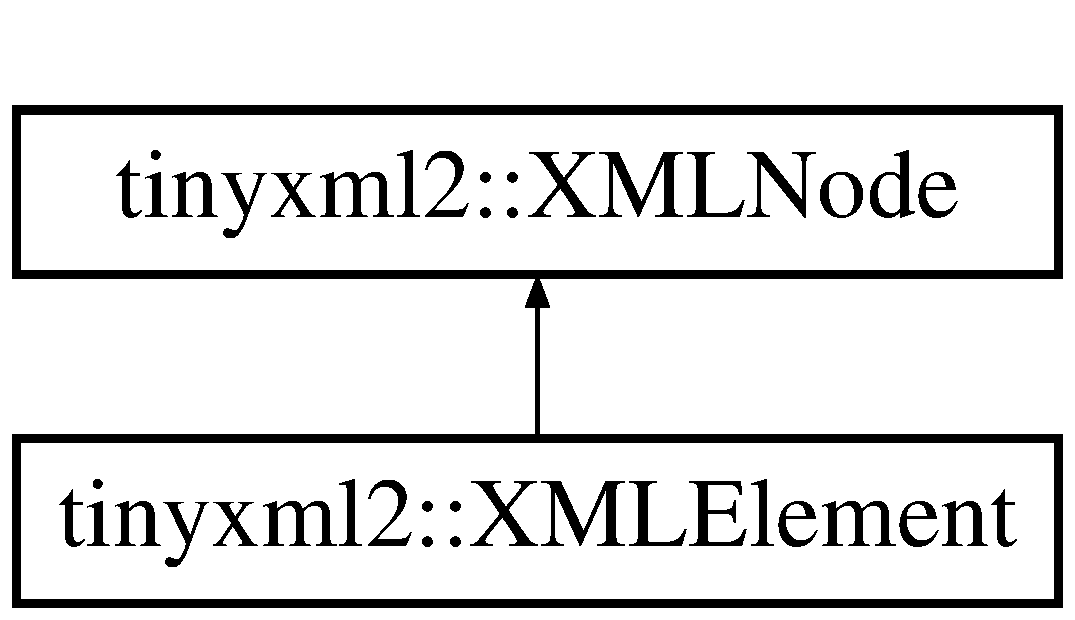
\includegraphics[height=2.000000cm]{classtinyxml2_1_1_x_m_l_element}
\end{center}
\end{figure}
\subsection*{Public Types}
\begin{DoxyCompactItemize}
\item 
enum \mbox{\hyperlink{classtinyxml2_1_1_x_m_l_element_ab5f90e2493c35702175235127e2935b4}{Element\+Closing\+Type}} \{ \mbox{\hyperlink{classtinyxml2_1_1_x_m_l_element_ab5f90e2493c35702175235127e2935b4a78cf277c55b4655c86458dfecb11d349}{O\+P\+EN}}, 
\mbox{\hyperlink{classtinyxml2_1_1_x_m_l_element_ab5f90e2493c35702175235127e2935b4aa2f1f384020d2d4538ad2ec84930a028}{C\+L\+O\+S\+ED}}, 
\mbox{\hyperlink{classtinyxml2_1_1_x_m_l_element_ab5f90e2493c35702175235127e2935b4aa2857344b98a931536c443cd0cadc4b7}{C\+L\+O\+S\+I\+NG}}
 \}
\end{DoxyCompactItemize}
\subsection*{Public Member Functions}
\begin{DoxyCompactItemize}
\item 
const char $\ast$ \mbox{\hyperlink{classtinyxml2_1_1_x_m_l_element_a63e057fb5baee1dd29f323cb85907b35}{Name}} () const
\begin{DoxyCompactList}\small\item\em Get the name of an element (which is the \mbox{\hyperlink{classtinyxml2_1_1_x_m_l_node_a0485e51c670e741884cfd8362274d680}{Value()}} of the node.) \end{DoxyCompactList}\item 
void \mbox{\hyperlink{classtinyxml2_1_1_x_m_l_element_a97712009a530d8cb8a63bf705f02b4f1}{Set\+Name}} (const char $\ast$str, bool static\+Mem=false)
\begin{DoxyCompactList}\small\item\em Set the name of the element. \end{DoxyCompactList}\item 
virtual \mbox{\hyperlink{classtinyxml2_1_1_x_m_l_element}{X\+M\+L\+Element}} $\ast$ \mbox{\hyperlink{classtinyxml2_1_1_x_m_l_element_ad9ff5c2dbc15df36cf664ce1b0ea0a5d}{To\+Element}} ()
\begin{DoxyCompactList}\small\item\em Safely cast to an Element, or null. \end{DoxyCompactList}\item 
virtual const \mbox{\hyperlink{classtinyxml2_1_1_x_m_l_element}{X\+M\+L\+Element}} $\ast$ \mbox{\hyperlink{classtinyxml2_1_1_x_m_l_element_afeb353047ab8532191709dcaef07337e}{To\+Element}} () const
\item 
virtual bool \mbox{\hyperlink{classtinyxml2_1_1_x_m_l_element_a9b2119831e8b85827d5d3e5076788e4a}{Accept}} (\mbox{\hyperlink{classtinyxml2_1_1_x_m_l_visitor}{X\+M\+L\+Visitor}} $\ast$visitor) const
\item 
const char $\ast$ \mbox{\hyperlink{classtinyxml2_1_1_x_m_l_element_a48cf4a315cfbac7d74cd0d5ff2c5df51}{Attribute}} (const char $\ast$name, const char $\ast$value=0) const
\item 
int \mbox{\hyperlink{classtinyxml2_1_1_x_m_l_element_a95a89b13bb14a2d4655e2b5b406c00d4}{Int\+Attribute}} (const char $\ast$name, int default\+Value=0) const
\item 
unsigned \mbox{\hyperlink{classtinyxml2_1_1_x_m_l_element_afea43a1d4aa33e3703ddee5fc9adc26c}{Unsigned\+Attribute}} (const char $\ast$name, unsigned default\+Value=0) const
\begin{DoxyCompactList}\small\item\em See \mbox{\hyperlink{classtinyxml2_1_1_x_m_l_element_a95a89b13bb14a2d4655e2b5b406c00d4}{Int\+Attribute()}} \end{DoxyCompactList}\item 
int64\+\_\+t \mbox{\hyperlink{classtinyxml2_1_1_x_m_l_element_a66d96972adecd816194191f13cc4a0a0}{Int64\+Attribute}} (const char $\ast$name, int64\+\_\+t default\+Value=0) const
\begin{DoxyCompactList}\small\item\em See \mbox{\hyperlink{classtinyxml2_1_1_x_m_l_element_a95a89b13bb14a2d4655e2b5b406c00d4}{Int\+Attribute()}} \end{DoxyCompactList}\item 
bool \mbox{\hyperlink{classtinyxml2_1_1_x_m_l_element_a53eda26131e1ad1031ef8ec8adb51bd8}{Bool\+Attribute}} (const char $\ast$name, bool default\+Value=false) const
\begin{DoxyCompactList}\small\item\em See \mbox{\hyperlink{classtinyxml2_1_1_x_m_l_element_a95a89b13bb14a2d4655e2b5b406c00d4}{Int\+Attribute()}} \end{DoxyCompactList}\item 
double \mbox{\hyperlink{classtinyxml2_1_1_x_m_l_element_a10a90c505aea716bf073eea1c97f33b5}{Double\+Attribute}} (const char $\ast$name, double default\+Value=0) const
\begin{DoxyCompactList}\small\item\em See \mbox{\hyperlink{classtinyxml2_1_1_x_m_l_element_a95a89b13bb14a2d4655e2b5b406c00d4}{Int\+Attribute()}} \end{DoxyCompactList}\item 
float \mbox{\hyperlink{classtinyxml2_1_1_x_m_l_element_ab1f4be2332e27dc640e9b6abd01d64dd}{Float\+Attribute}} (const char $\ast$name, float default\+Value=0) const
\begin{DoxyCompactList}\small\item\em See \mbox{\hyperlink{classtinyxml2_1_1_x_m_l_element_a95a89b13bb14a2d4655e2b5b406c00d4}{Int\+Attribute()}} \end{DoxyCompactList}\item 
\mbox{\hyperlink{namespacetinyxml2_a1fbf88509c3ac88c09117b1947414e08}{X\+M\+L\+Error}} \mbox{\hyperlink{classtinyxml2_1_1_x_m_l_element_a8a78bc1187c1c45ad89f2690eab567b1}{Query\+Int\+Attribute}} (const char $\ast$name, int $\ast$value) const
\item 
\mbox{\hyperlink{namespacetinyxml2_a1fbf88509c3ac88c09117b1947414e08}{X\+M\+L\+Error}} \mbox{\hyperlink{classtinyxml2_1_1_x_m_l_element_a26fc84cbfba6769dafcfbf256c05e22f}{Query\+Unsigned\+Attribute}} (const char $\ast$name, unsigned int $\ast$value) const
\begin{DoxyCompactList}\small\item\em See \mbox{\hyperlink{classtinyxml2_1_1_x_m_l_element_a8a78bc1187c1c45ad89f2690eab567b1}{Query\+Int\+Attribute()}} \end{DoxyCompactList}\item 
\mbox{\hyperlink{namespacetinyxml2_a1fbf88509c3ac88c09117b1947414e08}{X\+M\+L\+Error}} \mbox{\hyperlink{classtinyxml2_1_1_x_m_l_element_a7c0955d80b6f8d196744eacb0f6e90a8}{Query\+Int64\+Attribute}} (const char $\ast$name, int64\+\_\+t $\ast$value) const
\begin{DoxyCompactList}\small\item\em See \mbox{\hyperlink{classtinyxml2_1_1_x_m_l_element_a8a78bc1187c1c45ad89f2690eab567b1}{Query\+Int\+Attribute()}} \end{DoxyCompactList}\item 
\mbox{\hyperlink{namespacetinyxml2_a1fbf88509c3ac88c09117b1947414e08}{X\+M\+L\+Error}} \mbox{\hyperlink{classtinyxml2_1_1_x_m_l_element_a14c1bb77c39689838be01838d86ca872}{Query\+Bool\+Attribute}} (const char $\ast$name, bool $\ast$value) const
\begin{DoxyCompactList}\small\item\em See \mbox{\hyperlink{classtinyxml2_1_1_x_m_l_element_a8a78bc1187c1c45ad89f2690eab567b1}{Query\+Int\+Attribute()}} \end{DoxyCompactList}\item 
\mbox{\hyperlink{namespacetinyxml2_a1fbf88509c3ac88c09117b1947414e08}{X\+M\+L\+Error}} \mbox{\hyperlink{classtinyxml2_1_1_x_m_l_element_a5f0964e2dbd8e2ee7fce9beab689443c}{Query\+Double\+Attribute}} (const char $\ast$name, double $\ast$value) const
\begin{DoxyCompactList}\small\item\em See \mbox{\hyperlink{classtinyxml2_1_1_x_m_l_element_a8a78bc1187c1c45ad89f2690eab567b1}{Query\+Int\+Attribute()}} \end{DoxyCompactList}\item 
\mbox{\hyperlink{namespacetinyxml2_a1fbf88509c3ac88c09117b1947414e08}{X\+M\+L\+Error}} \mbox{\hyperlink{classtinyxml2_1_1_x_m_l_element_acd5eeddf6002ef90806af794b9d9a5a5}{Query\+Float\+Attribute}} (const char $\ast$name, float $\ast$value) const
\begin{DoxyCompactList}\small\item\em See \mbox{\hyperlink{classtinyxml2_1_1_x_m_l_element_a8a78bc1187c1c45ad89f2690eab567b1}{Query\+Int\+Attribute()}} \end{DoxyCompactList}\item 
\mbox{\hyperlink{namespacetinyxml2_a1fbf88509c3ac88c09117b1947414e08}{X\+M\+L\+Error}} \mbox{\hyperlink{classtinyxml2_1_1_x_m_l_element_adb8ae765f98d0c5037faec48deea78bc}{Query\+String\+Attribute}} (const char $\ast$name, const char $\ast$$\ast$value) const
\begin{DoxyCompactList}\small\item\em See \mbox{\hyperlink{classtinyxml2_1_1_x_m_l_element_a8a78bc1187c1c45ad89f2690eab567b1}{Query\+Int\+Attribute()}} \end{DoxyCompactList}\item 
\mbox{\hyperlink{namespacetinyxml2_a1fbf88509c3ac88c09117b1947414e08}{X\+M\+L\+Error}} \mbox{\hyperlink{classtinyxml2_1_1_x_m_l_element_a5b7df3bed2b8954eabf227fa204522eb}{Query\+Attribute}} (const char $\ast$name, int $\ast$value) const
\item 
\mbox{\hyperlink{namespacetinyxml2_a1fbf88509c3ac88c09117b1947414e08}{X\+M\+L\+Error}} \mbox{\hyperlink{classtinyxml2_1_1_x_m_l_element_a432276ea6e034cad19ad66de887ee13c}{Query\+Attribute}} (const char $\ast$name, unsigned int $\ast$value) const
\item 
\mbox{\hyperlink{namespacetinyxml2_a1fbf88509c3ac88c09117b1947414e08}{X\+M\+L\+Error}} \mbox{\hyperlink{classtinyxml2_1_1_x_m_l_element_a4867aea7a812acf7f00a915e4eaeaf3e}{Query\+Attribute}} (const char $\ast$name, int64\+\_\+t $\ast$value) const
\item 
\mbox{\hyperlink{namespacetinyxml2_a1fbf88509c3ac88c09117b1947414e08}{X\+M\+L\+Error}} \mbox{\hyperlink{classtinyxml2_1_1_x_m_l_element_a17139a22f2552439a7c2780e8e901522}{Query\+Attribute}} (const char $\ast$name, bool $\ast$value) const
\item 
\mbox{\hyperlink{namespacetinyxml2_a1fbf88509c3ac88c09117b1947414e08}{X\+M\+L\+Error}} \mbox{\hyperlink{classtinyxml2_1_1_x_m_l_element_a4f4da49900e82e25d163a7c0325fcc5f}{Query\+Attribute}} (const char $\ast$name, double $\ast$value) const
\item 
\mbox{\hyperlink{namespacetinyxml2_a1fbf88509c3ac88c09117b1947414e08}{X\+M\+L\+Error}} \mbox{\hyperlink{classtinyxml2_1_1_x_m_l_element_ac85b18ccd9ee8a79a2fd97cc593aae43}{Query\+Attribute}} (const char $\ast$name, float $\ast$value) const
\item 
void \mbox{\hyperlink{classtinyxml2_1_1_x_m_l_element_a11943abf2d0831548c3790dd5d9f119c}{Set\+Attribute}} (const char $\ast$name, const char $\ast$value)
\begin{DoxyCompactList}\small\item\em Sets the named attribute to value. \end{DoxyCompactList}\item 
void \mbox{\hyperlink{classtinyxml2_1_1_x_m_l_element_aae6568c64c7f1cc88be8461ba41a79cf}{Set\+Attribute}} (const char $\ast$name, int value)
\begin{DoxyCompactList}\small\item\em Sets the named attribute to value. \end{DoxyCompactList}\item 
void \mbox{\hyperlink{classtinyxml2_1_1_x_m_l_element_ae143997e90064ba82326b29a9930ea8f}{Set\+Attribute}} (const char $\ast$name, unsigned value)
\begin{DoxyCompactList}\small\item\em Sets the named attribute to value. \end{DoxyCompactList}\item 
void \mbox{\hyperlink{classtinyxml2_1_1_x_m_l_element_aaeefdf9171fec91b13a776b42299b0dd}{Set\+Attribute}} (const char $\ast$name, int64\+\_\+t value)
\begin{DoxyCompactList}\small\item\em Sets the named attribute to value. \end{DoxyCompactList}\item 
void \mbox{\hyperlink{classtinyxml2_1_1_x_m_l_element_aa848b696e6a75e4e545c6da9893b11e1}{Set\+Attribute}} (const char $\ast$name, bool value)
\begin{DoxyCompactList}\small\item\em Sets the named attribute to value. \end{DoxyCompactList}\item 
void \mbox{\hyperlink{classtinyxml2_1_1_x_m_l_element_a233397ee81e70eb5d4b814c5f8698533}{Set\+Attribute}} (const char $\ast$name, double value)
\begin{DoxyCompactList}\small\item\em Sets the named attribute to value. \end{DoxyCompactList}\item 
void \mbox{\hyperlink{classtinyxml2_1_1_x_m_l_element_a554b70d882e65b28fc084b23df9b9759}{Set\+Attribute}} (const char $\ast$name, float value)
\begin{DoxyCompactList}\small\item\em Sets the named attribute to value. \end{DoxyCompactList}\item 
void \mbox{\hyperlink{classtinyxml2_1_1_x_m_l_element_aebd45aa7118964c30b32fe12e944628a}{Delete\+Attribute}} (const char $\ast$name)
\item 
const \mbox{\hyperlink{classtinyxml2_1_1_x_m_l_attribute}{X\+M\+L\+Attribute}} $\ast$ \mbox{\hyperlink{classtinyxml2_1_1_x_m_l_element_a3e191704c8d499906ec11fe2f60c6686}{First\+Attribute}} () const
\begin{DoxyCompactList}\small\item\em Return the first attribute in the list. \end{DoxyCompactList}\item 
const \mbox{\hyperlink{classtinyxml2_1_1_x_m_l_attribute}{X\+M\+L\+Attribute}} $\ast$ \mbox{\hyperlink{classtinyxml2_1_1_x_m_l_element_a157750dac8037a316fd1af1a973dfa2c}{Find\+Attribute}} (const char $\ast$name) const
\begin{DoxyCompactList}\small\item\em Query a specific attribute in the list. \end{DoxyCompactList}\item 
const char $\ast$ \mbox{\hyperlink{classtinyxml2_1_1_x_m_l_element_a0fa5bea0a4daf3ddd503dcabb823eba6}{Get\+Text}} () const
\item 
void \mbox{\hyperlink{classtinyxml2_1_1_x_m_l_element_a1f9c2cd61b72af5ae708d37b7ad283ce}{Set\+Text}} (const char $\ast$in\+Text)
\item 
void \mbox{\hyperlink{classtinyxml2_1_1_x_m_l_element_aeae8917b5ea6060b3c08d4e3d8d632d7}{Set\+Text}} (int value)
\begin{DoxyCompactList}\small\item\em Convenience method for setting text inside an element. See \mbox{\hyperlink{classtinyxml2_1_1_x_m_l_element_a1f9c2cd61b72af5ae708d37b7ad283ce}{Set\+Text()}} for important limitations. \end{DoxyCompactList}\item 
void \mbox{\hyperlink{classtinyxml2_1_1_x_m_l_element_a7bbfcc11d516598bc924a8fba4d08597}{Set\+Text}} (unsigned value)
\begin{DoxyCompactList}\small\item\em Convenience method for setting text inside an element. See \mbox{\hyperlink{classtinyxml2_1_1_x_m_l_element_a1f9c2cd61b72af5ae708d37b7ad283ce}{Set\+Text()}} for important limitations. \end{DoxyCompactList}\item 
void \mbox{\hyperlink{classtinyxml2_1_1_x_m_l_element_a7b62cd33acdfeff7ea2b1b330d4368e4}{Set\+Text}} (int64\+\_\+t value)
\begin{DoxyCompactList}\small\item\em Convenience method for setting text inside an element. See \mbox{\hyperlink{classtinyxml2_1_1_x_m_l_element_a1f9c2cd61b72af5ae708d37b7ad283ce}{Set\+Text()}} for important limitations. \end{DoxyCompactList}\item 
void \mbox{\hyperlink{classtinyxml2_1_1_x_m_l_element_ae4b543d6770de76fb6ab68e541c192a4}{Set\+Text}} (bool value)
\begin{DoxyCompactList}\small\item\em Convenience method for setting text inside an element. See \mbox{\hyperlink{classtinyxml2_1_1_x_m_l_element_a1f9c2cd61b72af5ae708d37b7ad283ce}{Set\+Text()}} for important limitations. \end{DoxyCompactList}\item 
void \mbox{\hyperlink{classtinyxml2_1_1_x_m_l_element_a67bd77ac9aaeff58ff20b4275a65ba4e}{Set\+Text}} (double value)
\begin{DoxyCompactList}\small\item\em Convenience method for setting text inside an element. See \mbox{\hyperlink{classtinyxml2_1_1_x_m_l_element_a1f9c2cd61b72af5ae708d37b7ad283ce}{Set\+Text()}} for important limitations. \end{DoxyCompactList}\item 
void \mbox{\hyperlink{classtinyxml2_1_1_x_m_l_element_a51d560da5ae3ad6b75e0ab9ffb2ae42a}{Set\+Text}} (float value)
\begin{DoxyCompactList}\small\item\em Convenience method for setting text inside an element. See \mbox{\hyperlink{classtinyxml2_1_1_x_m_l_element_a1f9c2cd61b72af5ae708d37b7ad283ce}{Set\+Text()}} for important limitations. \end{DoxyCompactList}\item 
\mbox{\hyperlink{namespacetinyxml2_a1fbf88509c3ac88c09117b1947414e08}{X\+M\+L\+Error}} \mbox{\hyperlink{classtinyxml2_1_1_x_m_l_element_a926357996bef633cb736e1a558419632}{Query\+Int\+Text}} (int $\ast$ival) const
\item 
\mbox{\hyperlink{namespacetinyxml2_a1fbf88509c3ac88c09117b1947414e08}{X\+M\+L\+Error}} \mbox{\hyperlink{classtinyxml2_1_1_x_m_l_element_a14d38aa4b5e18a46274a27425188a6a1}{Query\+Unsigned\+Text}} (unsigned $\ast$uval) const
\begin{DoxyCompactList}\small\item\em See \mbox{\hyperlink{classtinyxml2_1_1_x_m_l_element_a926357996bef633cb736e1a558419632}{Query\+Int\+Text()}} \end{DoxyCompactList}\item 
\mbox{\hyperlink{namespacetinyxml2_a1fbf88509c3ac88c09117b1947414e08}{X\+M\+L\+Error}} \mbox{\hyperlink{classtinyxml2_1_1_x_m_l_element_a120c538c8eead169e635dbc70fb226d8}{Query\+Int64\+Text}} (int64\+\_\+t $\ast$uval) const
\begin{DoxyCompactList}\small\item\em See \mbox{\hyperlink{classtinyxml2_1_1_x_m_l_element_a926357996bef633cb736e1a558419632}{Query\+Int\+Text()}} \end{DoxyCompactList}\item 
\mbox{\hyperlink{namespacetinyxml2_a1fbf88509c3ac88c09117b1947414e08}{X\+M\+L\+Error}} \mbox{\hyperlink{classtinyxml2_1_1_x_m_l_element_a3fe5417d59eb8f5c4afe924b7d332736}{Query\+Bool\+Text}} (bool $\ast$bval) const
\begin{DoxyCompactList}\small\item\em See \mbox{\hyperlink{classtinyxml2_1_1_x_m_l_element_a926357996bef633cb736e1a558419632}{Query\+Int\+Text()}} \end{DoxyCompactList}\item 
\mbox{\hyperlink{namespacetinyxml2_a1fbf88509c3ac88c09117b1947414e08}{X\+M\+L\+Error}} \mbox{\hyperlink{classtinyxml2_1_1_x_m_l_element_a684679c99bb036a25652744cec6c4d96}{Query\+Double\+Text}} (double $\ast$dval) const
\begin{DoxyCompactList}\small\item\em See \mbox{\hyperlink{classtinyxml2_1_1_x_m_l_element_a926357996bef633cb736e1a558419632}{Query\+Int\+Text()}} \end{DoxyCompactList}\item 
\mbox{\hyperlink{namespacetinyxml2_a1fbf88509c3ac88c09117b1947414e08}{X\+M\+L\+Error}} \mbox{\hyperlink{classtinyxml2_1_1_x_m_l_element_afa332afedd93210daa6d44b88eb11e29}{Query\+Float\+Text}} (float $\ast$fval) const
\begin{DoxyCompactList}\small\item\em See \mbox{\hyperlink{classtinyxml2_1_1_x_m_l_element_a926357996bef633cb736e1a558419632}{Query\+Int\+Text()}} \end{DoxyCompactList}\item 
int \mbox{\hyperlink{classtinyxml2_1_1_x_m_l_element_a37b0636adebb8a1a1bc965f60824cb3e}{Int\+Text}} (int default\+Value=0) const
\item 
unsigned \mbox{\hyperlink{classtinyxml2_1_1_x_m_l_element_a49bad014ffcc17b0b6119d5b2c97dfb5}{Unsigned\+Text}} (unsigned default\+Value=0) const
\begin{DoxyCompactList}\small\item\em See \mbox{\hyperlink{classtinyxml2_1_1_x_m_l_element_a926357996bef633cb736e1a558419632}{Query\+Int\+Text()}} \end{DoxyCompactList}\item 
int64\+\_\+t \mbox{\hyperlink{classtinyxml2_1_1_x_m_l_element_aab6151f7e3b4c2c0a8234e262d7b6b8a}{Int64\+Text}} (int64\+\_\+t default\+Value=0) const
\begin{DoxyCompactList}\small\item\em See \mbox{\hyperlink{classtinyxml2_1_1_x_m_l_element_a926357996bef633cb736e1a558419632}{Query\+Int\+Text()}} \end{DoxyCompactList}\item 
bool \mbox{\hyperlink{classtinyxml2_1_1_x_m_l_element_a68569f59f6382bcea7f5013ec59736d2}{Bool\+Text}} (bool default\+Value=false) const
\begin{DoxyCompactList}\small\item\em See \mbox{\hyperlink{classtinyxml2_1_1_x_m_l_element_a926357996bef633cb736e1a558419632}{Query\+Int\+Text()}} \end{DoxyCompactList}\item 
double \mbox{\hyperlink{classtinyxml2_1_1_x_m_l_element_a81b1ff0cf2f2cd09be8badc08b39a2b7}{Double\+Text}} (double default\+Value=0) const
\begin{DoxyCompactList}\small\item\em See \mbox{\hyperlink{classtinyxml2_1_1_x_m_l_element_a926357996bef633cb736e1a558419632}{Query\+Int\+Text()}} \end{DoxyCompactList}\item 
float \mbox{\hyperlink{classtinyxml2_1_1_x_m_l_element_a45444eb21f99ca46101545992dc2e927}{Float\+Text}} (float default\+Value=0) const
\begin{DoxyCompactList}\small\item\em See \mbox{\hyperlink{classtinyxml2_1_1_x_m_l_element_a926357996bef633cb736e1a558419632}{Query\+Int\+Text()}} \end{DoxyCompactList}\item 
\mbox{\hyperlink{classtinyxml2_1_1_x_m_l_element_ab5f90e2493c35702175235127e2935b4}{Element\+Closing\+Type}} \mbox{\hyperlink{classtinyxml2_1_1_x_m_l_element_a6965ff89557f27d4082d7043d5145555}{Closing\+Type}} () const
\item 
virtual \mbox{\hyperlink{classtinyxml2_1_1_x_m_l_node}{X\+M\+L\+Node}} $\ast$ \mbox{\hyperlink{classtinyxml2_1_1_x_m_l_element_aafa2807a45b28fe096b29d76e6a13b7c}{Shallow\+Clone}} (\mbox{\hyperlink{classtinyxml2_1_1_x_m_l_document}{X\+M\+L\+Document}} $\ast$document) const
\item 
virtual bool \mbox{\hyperlink{classtinyxml2_1_1_x_m_l_element_a61ffd7bf918a9db4aa6203d855ac5ec2}{Shallow\+Equal}} (const \mbox{\hyperlink{classtinyxml2_1_1_x_m_l_node}{X\+M\+L\+Node}} $\ast$compare) const
\end{DoxyCompactItemize}
\subsection*{Protected Member Functions}
\begin{DoxyCompactItemize}
\item 
char $\ast$ \mbox{\hyperlink{classtinyxml2_1_1_x_m_l_element_a072998100b7d0ba5e8aeac6dd6dfb31b}{Parse\+Deep}} (char $\ast$p, \mbox{\hyperlink{classtinyxml2_1_1_str_pair}{Str\+Pair}} $\ast$parent\+End\+Tag, int $\ast$cur\+Line\+Num\+Ptr)
\end{DoxyCompactItemize}
\subsection*{Friends}
\begin{DoxyCompactItemize}
\item 
class \mbox{\hyperlink{classtinyxml2_1_1_x_m_l_element_a4eee3bda60c60a30e4e8cd4ea91c4c6e}{X\+M\+L\+Document}}
\end{DoxyCompactItemize}
\subsection*{Additional Inherited Members}


\subsection{Detailed Description}
The element is a container class. It has a value, the element name, and can contain other elements, text, comments, and unknowns. Elements also contain an arbitrary number of attributes. 

\subsection{Member Enumeration Documentation}
\mbox{\Hypertarget{classtinyxml2_1_1_x_m_l_element_ab5f90e2493c35702175235127e2935b4}\label{classtinyxml2_1_1_x_m_l_element_ab5f90e2493c35702175235127e2935b4}} 
\index{tinyxml2\+::\+X\+M\+L\+Element@{tinyxml2\+::\+X\+M\+L\+Element}!Element\+Closing\+Type@{Element\+Closing\+Type}}
\index{Element\+Closing\+Type@{Element\+Closing\+Type}!tinyxml2\+::\+X\+M\+L\+Element@{tinyxml2\+::\+X\+M\+L\+Element}}
\subsubsection{\texorpdfstring{Element\+Closing\+Type}{ElementClosingType}}
{\footnotesize\ttfamily enum \mbox{\hyperlink{classtinyxml2_1_1_x_m_l_element_ab5f90e2493c35702175235127e2935b4}{tinyxml2\+::\+X\+M\+L\+Element\+::\+Element\+Closing\+Type}}}

\begin{DoxyEnumFields}{Enumerator}
\raisebox{\heightof{T}}[0pt][0pt]{\index{O\+P\+EN@{O\+P\+EN}!tinyxml2\+::\+X\+M\+L\+Element@{tinyxml2\+::\+X\+M\+L\+Element}}\index{tinyxml2\+::\+X\+M\+L\+Element@{tinyxml2\+::\+X\+M\+L\+Element}!O\+P\+EN@{O\+P\+EN}}}\mbox{\Hypertarget{classtinyxml2_1_1_x_m_l_element_ab5f90e2493c35702175235127e2935b4a78cf277c55b4655c86458dfecb11d349}\label{classtinyxml2_1_1_x_m_l_element_ab5f90e2493c35702175235127e2935b4a78cf277c55b4655c86458dfecb11d349}} 
O\+P\+EN&\\
\hline

\raisebox{\heightof{T}}[0pt][0pt]{\index{C\+L\+O\+S\+ED@{C\+L\+O\+S\+ED}!tinyxml2\+::\+X\+M\+L\+Element@{tinyxml2\+::\+X\+M\+L\+Element}}\index{tinyxml2\+::\+X\+M\+L\+Element@{tinyxml2\+::\+X\+M\+L\+Element}!C\+L\+O\+S\+ED@{C\+L\+O\+S\+ED}}}\mbox{\Hypertarget{classtinyxml2_1_1_x_m_l_element_ab5f90e2493c35702175235127e2935b4aa2f1f384020d2d4538ad2ec84930a028}\label{classtinyxml2_1_1_x_m_l_element_ab5f90e2493c35702175235127e2935b4aa2f1f384020d2d4538ad2ec84930a028}} 
C\+L\+O\+S\+ED&\\
\hline

\raisebox{\heightof{T}}[0pt][0pt]{\index{C\+L\+O\+S\+I\+NG@{C\+L\+O\+S\+I\+NG}!tinyxml2\+::\+X\+M\+L\+Element@{tinyxml2\+::\+X\+M\+L\+Element}}\index{tinyxml2\+::\+X\+M\+L\+Element@{tinyxml2\+::\+X\+M\+L\+Element}!C\+L\+O\+S\+I\+NG@{C\+L\+O\+S\+I\+NG}}}\mbox{\Hypertarget{classtinyxml2_1_1_x_m_l_element_ab5f90e2493c35702175235127e2935b4aa2857344b98a931536c443cd0cadc4b7}\label{classtinyxml2_1_1_x_m_l_element_ab5f90e2493c35702175235127e2935b4aa2857344b98a931536c443cd0cadc4b7}} 
C\+L\+O\+S\+I\+NG&\\
\hline

\end{DoxyEnumFields}


\subsection{Member Function Documentation}
\mbox{\Hypertarget{classtinyxml2_1_1_x_m_l_element_a9b2119831e8b85827d5d3e5076788e4a}\label{classtinyxml2_1_1_x_m_l_element_a9b2119831e8b85827d5d3e5076788e4a}} 
\index{tinyxml2\+::\+X\+M\+L\+Element@{tinyxml2\+::\+X\+M\+L\+Element}!Accept@{Accept}}
\index{Accept@{Accept}!tinyxml2\+::\+X\+M\+L\+Element@{tinyxml2\+::\+X\+M\+L\+Element}}
\subsubsection{\texorpdfstring{Accept()}{Accept()}}
{\footnotesize\ttfamily bool tinyxml2\+::\+X\+M\+L\+Element\+::\+Accept (\begin{DoxyParamCaption}\item[{\mbox{\hyperlink{classtinyxml2_1_1_x_m_l_visitor}{X\+M\+L\+Visitor}} $\ast$}]{visitor }\end{DoxyParamCaption}) const\hspace{0.3cm}{\ttfamily [virtual]}}

Accept a hierarchical visit of the nodes in the Tiny\+X\+M\+L-\/2 D\+OM. Every node in the X\+ML tree will be conditionally visited and the host will be called back via the \mbox{\hyperlink{classtinyxml2_1_1_x_m_l_visitor}{X\+M\+L\+Visitor}} interface.

This is essentially a S\+AX interface for Tiny\+X\+M\+L-\/2. (Note however it doesn\textquotesingle{}t re-\/parse the X\+ML for the callbacks, so the performance of Tiny\+X\+M\+L-\/2 is unchanged by using this interface versus any other.)

The interface has been based on ideas from\+:


\begin{DoxyItemize}
\item \href{http://www.saxproject.org/}{\tt http\+://www.\+saxproject.\+org/}
\item \href{http://c2.com/cgi/wiki?HierarchicalVisitorPattern}{\tt http\+://c2.\+com/cgi/wiki?\+Hierarchical\+Visitor\+Pattern}
\end{DoxyItemize}

Which are both good references for \char`\"{}visiting\char`\"{}.

An example of using \mbox{\hyperlink{classtinyxml2_1_1_x_m_l_element_a9b2119831e8b85827d5d3e5076788e4a}{Accept()}}\+: \begin{DoxyVerb}XMLPrinter printer;
tinyxmlDoc.Accept( &printer );
const char* xmlcstr = printer.CStr();
\end{DoxyVerb}
 

Implements \mbox{\hyperlink{classtinyxml2_1_1_x_m_l_node_a81e66df0a44c67a7af17f3b77a152785}{tinyxml2\+::\+X\+M\+L\+Node}}.

\mbox{\Hypertarget{classtinyxml2_1_1_x_m_l_element_a48cf4a315cfbac7d74cd0d5ff2c5df51}\label{classtinyxml2_1_1_x_m_l_element_a48cf4a315cfbac7d74cd0d5ff2c5df51}} 
\index{tinyxml2\+::\+X\+M\+L\+Element@{tinyxml2\+::\+X\+M\+L\+Element}!Attribute@{Attribute}}
\index{Attribute@{Attribute}!tinyxml2\+::\+X\+M\+L\+Element@{tinyxml2\+::\+X\+M\+L\+Element}}
\subsubsection{\texorpdfstring{Attribute()}{Attribute()}}
{\footnotesize\ttfamily const char $\ast$ tinyxml2\+::\+X\+M\+L\+Element\+::\+Attribute (\begin{DoxyParamCaption}\item[{const char $\ast$}]{name,  }\item[{const char $\ast$}]{value = {\ttfamily 0} }\end{DoxyParamCaption}) const}

Given an attribute name, \mbox{\hyperlink{classtinyxml2_1_1_x_m_l_element_a48cf4a315cfbac7d74cd0d5ff2c5df51}{Attribute()}} returns the value for the attribute of that name, or null if none exists. For example\+:

\begin{DoxyVerb}const char* value = ele->Attribute( "foo" );
\end{DoxyVerb}


The \textquotesingle{}value\textquotesingle{} parameter is normally null. However, if specified, the attribute will only be returned if the \textquotesingle{}name\textquotesingle{} and \textquotesingle{}value\textquotesingle{} match. This allow you to write code\+:

\begin{DoxyVerb}if ( ele->Attribute( "foo", "bar" ) ) callFooIsBar();
\end{DoxyVerb}


rather than\+: \begin{DoxyVerb}if ( ele->Attribute( "foo" ) ) {
    if ( strcmp( ele->Attribute( "foo" ), "bar" ) == 0 ) callFooIsBar();
}
\end{DoxyVerb}
 \mbox{\Hypertarget{classtinyxml2_1_1_x_m_l_element_a53eda26131e1ad1031ef8ec8adb51bd8}\label{classtinyxml2_1_1_x_m_l_element_a53eda26131e1ad1031ef8ec8adb51bd8}} 
\index{tinyxml2\+::\+X\+M\+L\+Element@{tinyxml2\+::\+X\+M\+L\+Element}!Bool\+Attribute@{Bool\+Attribute}}
\index{Bool\+Attribute@{Bool\+Attribute}!tinyxml2\+::\+X\+M\+L\+Element@{tinyxml2\+::\+X\+M\+L\+Element}}
\subsubsection{\texorpdfstring{Bool\+Attribute()}{BoolAttribute()}}
{\footnotesize\ttfamily bool tinyxml2\+::\+X\+M\+L\+Element\+::\+Bool\+Attribute (\begin{DoxyParamCaption}\item[{const char $\ast$}]{name,  }\item[{bool}]{default\+Value = {\ttfamily false} }\end{DoxyParamCaption}) const}



See \mbox{\hyperlink{classtinyxml2_1_1_x_m_l_element_a95a89b13bb14a2d4655e2b5b406c00d4}{Int\+Attribute()}} 

\mbox{\Hypertarget{classtinyxml2_1_1_x_m_l_element_a68569f59f6382bcea7f5013ec59736d2}\label{classtinyxml2_1_1_x_m_l_element_a68569f59f6382bcea7f5013ec59736d2}} 
\index{tinyxml2\+::\+X\+M\+L\+Element@{tinyxml2\+::\+X\+M\+L\+Element}!Bool\+Text@{Bool\+Text}}
\index{Bool\+Text@{Bool\+Text}!tinyxml2\+::\+X\+M\+L\+Element@{tinyxml2\+::\+X\+M\+L\+Element}}
\subsubsection{\texorpdfstring{Bool\+Text()}{BoolText()}}
{\footnotesize\ttfamily bool tinyxml2\+::\+X\+M\+L\+Element\+::\+Bool\+Text (\begin{DoxyParamCaption}\item[{bool}]{default\+Value = {\ttfamily false} }\end{DoxyParamCaption}) const}



See \mbox{\hyperlink{classtinyxml2_1_1_x_m_l_element_a926357996bef633cb736e1a558419632}{Query\+Int\+Text()}} 

\mbox{\Hypertarget{classtinyxml2_1_1_x_m_l_element_a6965ff89557f27d4082d7043d5145555}\label{classtinyxml2_1_1_x_m_l_element_a6965ff89557f27d4082d7043d5145555}} 
\index{tinyxml2\+::\+X\+M\+L\+Element@{tinyxml2\+::\+X\+M\+L\+Element}!Closing\+Type@{Closing\+Type}}
\index{Closing\+Type@{Closing\+Type}!tinyxml2\+::\+X\+M\+L\+Element@{tinyxml2\+::\+X\+M\+L\+Element}}
\subsubsection{\texorpdfstring{Closing\+Type()}{ClosingType()}}
{\footnotesize\ttfamily \mbox{\hyperlink{classtinyxml2_1_1_x_m_l_element_ab5f90e2493c35702175235127e2935b4}{Element\+Closing\+Type}} tinyxml2\+::\+X\+M\+L\+Element\+::\+Closing\+Type (\begin{DoxyParamCaption}{ }\end{DoxyParamCaption}) const\hspace{0.3cm}{\ttfamily [inline]}}

\mbox{\Hypertarget{classtinyxml2_1_1_x_m_l_element_aebd45aa7118964c30b32fe12e944628a}\label{classtinyxml2_1_1_x_m_l_element_aebd45aa7118964c30b32fe12e944628a}} 
\index{tinyxml2\+::\+X\+M\+L\+Element@{tinyxml2\+::\+X\+M\+L\+Element}!Delete\+Attribute@{Delete\+Attribute}}
\index{Delete\+Attribute@{Delete\+Attribute}!tinyxml2\+::\+X\+M\+L\+Element@{tinyxml2\+::\+X\+M\+L\+Element}}
\subsubsection{\texorpdfstring{Delete\+Attribute()}{DeleteAttribute()}}
{\footnotesize\ttfamily void tinyxml2\+::\+X\+M\+L\+Element\+::\+Delete\+Attribute (\begin{DoxyParamCaption}\item[{const char $\ast$}]{name }\end{DoxyParamCaption})}

Delete an attribute. \mbox{\Hypertarget{classtinyxml2_1_1_x_m_l_element_a10a90c505aea716bf073eea1c97f33b5}\label{classtinyxml2_1_1_x_m_l_element_a10a90c505aea716bf073eea1c97f33b5}} 
\index{tinyxml2\+::\+X\+M\+L\+Element@{tinyxml2\+::\+X\+M\+L\+Element}!Double\+Attribute@{Double\+Attribute}}
\index{Double\+Attribute@{Double\+Attribute}!tinyxml2\+::\+X\+M\+L\+Element@{tinyxml2\+::\+X\+M\+L\+Element}}
\subsubsection{\texorpdfstring{Double\+Attribute()}{DoubleAttribute()}}
{\footnotesize\ttfamily double tinyxml2\+::\+X\+M\+L\+Element\+::\+Double\+Attribute (\begin{DoxyParamCaption}\item[{const char $\ast$}]{name,  }\item[{double}]{default\+Value = {\ttfamily 0} }\end{DoxyParamCaption}) const}



See \mbox{\hyperlink{classtinyxml2_1_1_x_m_l_element_a95a89b13bb14a2d4655e2b5b406c00d4}{Int\+Attribute()}} 

\mbox{\Hypertarget{classtinyxml2_1_1_x_m_l_element_a81b1ff0cf2f2cd09be8badc08b39a2b7}\label{classtinyxml2_1_1_x_m_l_element_a81b1ff0cf2f2cd09be8badc08b39a2b7}} 
\index{tinyxml2\+::\+X\+M\+L\+Element@{tinyxml2\+::\+X\+M\+L\+Element}!Double\+Text@{Double\+Text}}
\index{Double\+Text@{Double\+Text}!tinyxml2\+::\+X\+M\+L\+Element@{tinyxml2\+::\+X\+M\+L\+Element}}
\subsubsection{\texorpdfstring{Double\+Text()}{DoubleText()}}
{\footnotesize\ttfamily double tinyxml2\+::\+X\+M\+L\+Element\+::\+Double\+Text (\begin{DoxyParamCaption}\item[{double}]{default\+Value = {\ttfamily 0} }\end{DoxyParamCaption}) const}



See \mbox{\hyperlink{classtinyxml2_1_1_x_m_l_element_a926357996bef633cb736e1a558419632}{Query\+Int\+Text()}} 

\mbox{\Hypertarget{classtinyxml2_1_1_x_m_l_element_a157750dac8037a316fd1af1a973dfa2c}\label{classtinyxml2_1_1_x_m_l_element_a157750dac8037a316fd1af1a973dfa2c}} 
\index{tinyxml2\+::\+X\+M\+L\+Element@{tinyxml2\+::\+X\+M\+L\+Element}!Find\+Attribute@{Find\+Attribute}}
\index{Find\+Attribute@{Find\+Attribute}!tinyxml2\+::\+X\+M\+L\+Element@{tinyxml2\+::\+X\+M\+L\+Element}}
\subsubsection{\texorpdfstring{Find\+Attribute()}{FindAttribute()}}
{\footnotesize\ttfamily const \mbox{\hyperlink{classtinyxml2_1_1_x_m_l_attribute}{X\+M\+L\+Attribute}} $\ast$ tinyxml2\+::\+X\+M\+L\+Element\+::\+Find\+Attribute (\begin{DoxyParamCaption}\item[{const char $\ast$}]{name }\end{DoxyParamCaption}) const}



Query a specific attribute in the list. 

\mbox{\Hypertarget{classtinyxml2_1_1_x_m_l_element_a3e191704c8d499906ec11fe2f60c6686}\label{classtinyxml2_1_1_x_m_l_element_a3e191704c8d499906ec11fe2f60c6686}} 
\index{tinyxml2\+::\+X\+M\+L\+Element@{tinyxml2\+::\+X\+M\+L\+Element}!First\+Attribute@{First\+Attribute}}
\index{First\+Attribute@{First\+Attribute}!tinyxml2\+::\+X\+M\+L\+Element@{tinyxml2\+::\+X\+M\+L\+Element}}
\subsubsection{\texorpdfstring{First\+Attribute()}{FirstAttribute()}}
{\footnotesize\ttfamily const \mbox{\hyperlink{classtinyxml2_1_1_x_m_l_attribute}{X\+M\+L\+Attribute}}$\ast$ tinyxml2\+::\+X\+M\+L\+Element\+::\+First\+Attribute (\begin{DoxyParamCaption}{ }\end{DoxyParamCaption}) const\hspace{0.3cm}{\ttfamily [inline]}}



Return the first attribute in the list. 

\mbox{\Hypertarget{classtinyxml2_1_1_x_m_l_element_ab1f4be2332e27dc640e9b6abd01d64dd}\label{classtinyxml2_1_1_x_m_l_element_ab1f4be2332e27dc640e9b6abd01d64dd}} 
\index{tinyxml2\+::\+X\+M\+L\+Element@{tinyxml2\+::\+X\+M\+L\+Element}!Float\+Attribute@{Float\+Attribute}}
\index{Float\+Attribute@{Float\+Attribute}!tinyxml2\+::\+X\+M\+L\+Element@{tinyxml2\+::\+X\+M\+L\+Element}}
\subsubsection{\texorpdfstring{Float\+Attribute()}{FloatAttribute()}}
{\footnotesize\ttfamily float tinyxml2\+::\+X\+M\+L\+Element\+::\+Float\+Attribute (\begin{DoxyParamCaption}\item[{const char $\ast$}]{name,  }\item[{float}]{default\+Value = {\ttfamily 0} }\end{DoxyParamCaption}) const}



See \mbox{\hyperlink{classtinyxml2_1_1_x_m_l_element_a95a89b13bb14a2d4655e2b5b406c00d4}{Int\+Attribute()}} 

\mbox{\Hypertarget{classtinyxml2_1_1_x_m_l_element_a45444eb21f99ca46101545992dc2e927}\label{classtinyxml2_1_1_x_m_l_element_a45444eb21f99ca46101545992dc2e927}} 
\index{tinyxml2\+::\+X\+M\+L\+Element@{tinyxml2\+::\+X\+M\+L\+Element}!Float\+Text@{Float\+Text}}
\index{Float\+Text@{Float\+Text}!tinyxml2\+::\+X\+M\+L\+Element@{tinyxml2\+::\+X\+M\+L\+Element}}
\subsubsection{\texorpdfstring{Float\+Text()}{FloatText()}}
{\footnotesize\ttfamily float tinyxml2\+::\+X\+M\+L\+Element\+::\+Float\+Text (\begin{DoxyParamCaption}\item[{float}]{default\+Value = {\ttfamily 0} }\end{DoxyParamCaption}) const}



See \mbox{\hyperlink{classtinyxml2_1_1_x_m_l_element_a926357996bef633cb736e1a558419632}{Query\+Int\+Text()}} 

\mbox{\Hypertarget{classtinyxml2_1_1_x_m_l_element_a0fa5bea0a4daf3ddd503dcabb823eba6}\label{classtinyxml2_1_1_x_m_l_element_a0fa5bea0a4daf3ddd503dcabb823eba6}} 
\index{tinyxml2\+::\+X\+M\+L\+Element@{tinyxml2\+::\+X\+M\+L\+Element}!Get\+Text@{Get\+Text}}
\index{Get\+Text@{Get\+Text}!tinyxml2\+::\+X\+M\+L\+Element@{tinyxml2\+::\+X\+M\+L\+Element}}
\subsubsection{\texorpdfstring{Get\+Text()}{GetText()}}
{\footnotesize\ttfamily const char $\ast$ tinyxml2\+::\+X\+M\+L\+Element\+::\+Get\+Text (\begin{DoxyParamCaption}{ }\end{DoxyParamCaption}) const}

Convenience function for easy access to the text inside an element. Although easy and concise, \mbox{\hyperlink{classtinyxml2_1_1_x_m_l_element_a0fa5bea0a4daf3ddd503dcabb823eba6}{Get\+Text()}} is limited compared to getting the \mbox{\hyperlink{classtinyxml2_1_1_x_m_l_text}{X\+M\+L\+Text}} child and accessing it directly.

If the first child of \textquotesingle{}this\textquotesingle{} is a \mbox{\hyperlink{classtinyxml2_1_1_x_m_l_text}{X\+M\+L\+Text}}, the \mbox{\hyperlink{classtinyxml2_1_1_x_m_l_element_a0fa5bea0a4daf3ddd503dcabb823eba6}{Get\+Text()}} returns the character string of the Text node, else null is returned.

This is a convenient method for getting the text of simple contained text\+: \begin{DoxyVerb}<foo>This is text</foo>
    const char* str = fooElement->GetText();
\end{DoxyVerb}


\textquotesingle{}str\textquotesingle{} will be a pointer to \char`\"{}\+This is text\char`\"{}.

Note that this function can be misleading. If the element foo was created from this X\+ML\+: \begin{DoxyVerb}    <foo><b>This is text</b></foo>
\end{DoxyVerb}


then the value of str would be null. The first child node isn\textquotesingle{}t a text node, it is another element. From this X\+ML\+: \begin{DoxyVerb}    <foo>This is <b>text</b></foo>
\end{DoxyVerb}
 \mbox{\hyperlink{classtinyxml2_1_1_x_m_l_element_a0fa5bea0a4daf3ddd503dcabb823eba6}{Get\+Text()}} will return \char`\"{}\+This is \char`\"{}. \mbox{\Hypertarget{classtinyxml2_1_1_x_m_l_element_a66d96972adecd816194191f13cc4a0a0}\label{classtinyxml2_1_1_x_m_l_element_a66d96972adecd816194191f13cc4a0a0}} 
\index{tinyxml2\+::\+X\+M\+L\+Element@{tinyxml2\+::\+X\+M\+L\+Element}!Int64\+Attribute@{Int64\+Attribute}}
\index{Int64\+Attribute@{Int64\+Attribute}!tinyxml2\+::\+X\+M\+L\+Element@{tinyxml2\+::\+X\+M\+L\+Element}}
\subsubsection{\texorpdfstring{Int64\+Attribute()}{Int64Attribute()}}
{\footnotesize\ttfamily int64\+\_\+t tinyxml2\+::\+X\+M\+L\+Element\+::\+Int64\+Attribute (\begin{DoxyParamCaption}\item[{const char $\ast$}]{name,  }\item[{int64\+\_\+t}]{default\+Value = {\ttfamily 0} }\end{DoxyParamCaption}) const}



See \mbox{\hyperlink{classtinyxml2_1_1_x_m_l_element_a95a89b13bb14a2d4655e2b5b406c00d4}{Int\+Attribute()}} 

\mbox{\Hypertarget{classtinyxml2_1_1_x_m_l_element_aab6151f7e3b4c2c0a8234e262d7b6b8a}\label{classtinyxml2_1_1_x_m_l_element_aab6151f7e3b4c2c0a8234e262d7b6b8a}} 
\index{tinyxml2\+::\+X\+M\+L\+Element@{tinyxml2\+::\+X\+M\+L\+Element}!Int64\+Text@{Int64\+Text}}
\index{Int64\+Text@{Int64\+Text}!tinyxml2\+::\+X\+M\+L\+Element@{tinyxml2\+::\+X\+M\+L\+Element}}
\subsubsection{\texorpdfstring{Int64\+Text()}{Int64Text()}}
{\footnotesize\ttfamily int64\+\_\+t tinyxml2\+::\+X\+M\+L\+Element\+::\+Int64\+Text (\begin{DoxyParamCaption}\item[{int64\+\_\+t}]{default\+Value = {\ttfamily 0} }\end{DoxyParamCaption}) const}



See \mbox{\hyperlink{classtinyxml2_1_1_x_m_l_element_a926357996bef633cb736e1a558419632}{Query\+Int\+Text()}} 

\mbox{\Hypertarget{classtinyxml2_1_1_x_m_l_element_a95a89b13bb14a2d4655e2b5b406c00d4}\label{classtinyxml2_1_1_x_m_l_element_a95a89b13bb14a2d4655e2b5b406c00d4}} 
\index{tinyxml2\+::\+X\+M\+L\+Element@{tinyxml2\+::\+X\+M\+L\+Element}!Int\+Attribute@{Int\+Attribute}}
\index{Int\+Attribute@{Int\+Attribute}!tinyxml2\+::\+X\+M\+L\+Element@{tinyxml2\+::\+X\+M\+L\+Element}}
\subsubsection{\texorpdfstring{Int\+Attribute()}{IntAttribute()}}
{\footnotesize\ttfamily int tinyxml2\+::\+X\+M\+L\+Element\+::\+Int\+Attribute (\begin{DoxyParamCaption}\item[{const char $\ast$}]{name,  }\item[{int}]{default\+Value = {\ttfamily 0} }\end{DoxyParamCaption}) const}

Given an attribute name, \mbox{\hyperlink{classtinyxml2_1_1_x_m_l_element_a95a89b13bb14a2d4655e2b5b406c00d4}{Int\+Attribute()}} returns the value of the attribute interpreted as an integer. The default value will be returned if the attribute isn\textquotesingle{}t present, or if there is an error. (For a method with error checking, see \mbox{\hyperlink{classtinyxml2_1_1_x_m_l_element_a8a78bc1187c1c45ad89f2690eab567b1}{Query\+Int\+Attribute()}}). \mbox{\Hypertarget{classtinyxml2_1_1_x_m_l_element_a37b0636adebb8a1a1bc965f60824cb3e}\label{classtinyxml2_1_1_x_m_l_element_a37b0636adebb8a1a1bc965f60824cb3e}} 
\index{tinyxml2\+::\+X\+M\+L\+Element@{tinyxml2\+::\+X\+M\+L\+Element}!Int\+Text@{Int\+Text}}
\index{Int\+Text@{Int\+Text}!tinyxml2\+::\+X\+M\+L\+Element@{tinyxml2\+::\+X\+M\+L\+Element}}
\subsubsection{\texorpdfstring{Int\+Text()}{IntText()}}
{\footnotesize\ttfamily int tinyxml2\+::\+X\+M\+L\+Element\+::\+Int\+Text (\begin{DoxyParamCaption}\item[{int}]{default\+Value = {\ttfamily 0} }\end{DoxyParamCaption}) const}

\mbox{\Hypertarget{classtinyxml2_1_1_x_m_l_element_a63e057fb5baee1dd29f323cb85907b35}\label{classtinyxml2_1_1_x_m_l_element_a63e057fb5baee1dd29f323cb85907b35}} 
\index{tinyxml2\+::\+X\+M\+L\+Element@{tinyxml2\+::\+X\+M\+L\+Element}!Name@{Name}}
\index{Name@{Name}!tinyxml2\+::\+X\+M\+L\+Element@{tinyxml2\+::\+X\+M\+L\+Element}}
\subsubsection{\texorpdfstring{Name()}{Name()}}
{\footnotesize\ttfamily const char$\ast$ tinyxml2\+::\+X\+M\+L\+Element\+::\+Name (\begin{DoxyParamCaption}{ }\end{DoxyParamCaption}) const\hspace{0.3cm}{\ttfamily [inline]}}



Get the name of an element (which is the \mbox{\hyperlink{classtinyxml2_1_1_x_m_l_node_a0485e51c670e741884cfd8362274d680}{Value()}} of the node.) 

\mbox{\Hypertarget{classtinyxml2_1_1_x_m_l_element_a072998100b7d0ba5e8aeac6dd6dfb31b}\label{classtinyxml2_1_1_x_m_l_element_a072998100b7d0ba5e8aeac6dd6dfb31b}} 
\index{tinyxml2\+::\+X\+M\+L\+Element@{tinyxml2\+::\+X\+M\+L\+Element}!Parse\+Deep@{Parse\+Deep}}
\index{Parse\+Deep@{Parse\+Deep}!tinyxml2\+::\+X\+M\+L\+Element@{tinyxml2\+::\+X\+M\+L\+Element}}
\subsubsection{\texorpdfstring{Parse\+Deep()}{ParseDeep()}}
{\footnotesize\ttfamily char $\ast$ tinyxml2\+::\+X\+M\+L\+Element\+::\+Parse\+Deep (\begin{DoxyParamCaption}\item[{char $\ast$}]{p,  }\item[{\mbox{\hyperlink{classtinyxml2_1_1_str_pair}{Str\+Pair}} $\ast$}]{parent\+End\+Tag,  }\item[{int $\ast$}]{cur\+Line\+Num\+Ptr }\end{DoxyParamCaption})\hspace{0.3cm}{\ttfamily [protected]}, {\ttfamily [virtual]}}



Reimplemented from \mbox{\hyperlink{classtinyxml2_1_1_x_m_l_node_a916e498914baecbc9a1f012352ef7c69}{tinyxml2\+::\+X\+M\+L\+Node}}.

\mbox{\Hypertarget{classtinyxml2_1_1_x_m_l_element_a5b7df3bed2b8954eabf227fa204522eb}\label{classtinyxml2_1_1_x_m_l_element_a5b7df3bed2b8954eabf227fa204522eb}} 
\index{tinyxml2\+::\+X\+M\+L\+Element@{tinyxml2\+::\+X\+M\+L\+Element}!Query\+Attribute@{Query\+Attribute}}
\index{Query\+Attribute@{Query\+Attribute}!tinyxml2\+::\+X\+M\+L\+Element@{tinyxml2\+::\+X\+M\+L\+Element}}
\subsubsection{\texorpdfstring{Query\+Attribute()}{QueryAttribute()}\hspace{0.1cm}{\footnotesize\ttfamily [1/6]}}
{\footnotesize\ttfamily \mbox{\hyperlink{namespacetinyxml2_a1fbf88509c3ac88c09117b1947414e08}{X\+M\+L\+Error}} tinyxml2\+::\+X\+M\+L\+Element\+::\+Query\+Attribute (\begin{DoxyParamCaption}\item[{const char $\ast$}]{name,  }\item[{int $\ast$}]{value }\end{DoxyParamCaption}) const\hspace{0.3cm}{\ttfamily [inline]}}

Given an attribute name, \mbox{\hyperlink{classtinyxml2_1_1_x_m_l_element_a5b7df3bed2b8954eabf227fa204522eb}{Query\+Attribute()}} returns X\+M\+L\+\_\+\+S\+U\+C\+C\+E\+SS, X\+M\+L\+\_\+\+W\+R\+O\+N\+G\+\_\+\+A\+T\+T\+R\+I\+B\+U\+T\+E\+\_\+\+T\+Y\+PE if the conversion can\textquotesingle{}t be performed, or X\+M\+L\+\_\+\+N\+O\+\_\+\+A\+T\+T\+R\+I\+B\+U\+TE if the attribute doesn\textquotesingle{}t exist. It is overloaded for the primitive types, and is a generally more convenient replacement of \mbox{\hyperlink{classtinyxml2_1_1_x_m_l_element_a8a78bc1187c1c45ad89f2690eab567b1}{Query\+Int\+Attribute()}} and related functions.

If successful, the result of the conversion will be written to \textquotesingle{}value\textquotesingle{}. If not successful, nothing will be written to \textquotesingle{}value\textquotesingle{}. This allows you to provide default value\+:

\begin{DoxyVerb}int value = 10;
QueryAttribute( "foo", &value );        // if "foo" isn't found, value will still be 10
\end{DoxyVerb}
 \mbox{\Hypertarget{classtinyxml2_1_1_x_m_l_element_a432276ea6e034cad19ad66de887ee13c}\label{classtinyxml2_1_1_x_m_l_element_a432276ea6e034cad19ad66de887ee13c}} 
\index{tinyxml2\+::\+X\+M\+L\+Element@{tinyxml2\+::\+X\+M\+L\+Element}!Query\+Attribute@{Query\+Attribute}}
\index{Query\+Attribute@{Query\+Attribute}!tinyxml2\+::\+X\+M\+L\+Element@{tinyxml2\+::\+X\+M\+L\+Element}}
\subsubsection{\texorpdfstring{Query\+Attribute()}{QueryAttribute()}\hspace{0.1cm}{\footnotesize\ttfamily [2/6]}}
{\footnotesize\ttfamily \mbox{\hyperlink{namespacetinyxml2_a1fbf88509c3ac88c09117b1947414e08}{X\+M\+L\+Error}} tinyxml2\+::\+X\+M\+L\+Element\+::\+Query\+Attribute (\begin{DoxyParamCaption}\item[{const char $\ast$}]{name,  }\item[{unsigned int $\ast$}]{value }\end{DoxyParamCaption}) const\hspace{0.3cm}{\ttfamily [inline]}}

\mbox{\Hypertarget{classtinyxml2_1_1_x_m_l_element_a4867aea7a812acf7f00a915e4eaeaf3e}\label{classtinyxml2_1_1_x_m_l_element_a4867aea7a812acf7f00a915e4eaeaf3e}} 
\index{tinyxml2\+::\+X\+M\+L\+Element@{tinyxml2\+::\+X\+M\+L\+Element}!Query\+Attribute@{Query\+Attribute}}
\index{Query\+Attribute@{Query\+Attribute}!tinyxml2\+::\+X\+M\+L\+Element@{tinyxml2\+::\+X\+M\+L\+Element}}
\subsubsection{\texorpdfstring{Query\+Attribute()}{QueryAttribute()}\hspace{0.1cm}{\footnotesize\ttfamily [3/6]}}
{\footnotesize\ttfamily \mbox{\hyperlink{namespacetinyxml2_a1fbf88509c3ac88c09117b1947414e08}{X\+M\+L\+Error}} tinyxml2\+::\+X\+M\+L\+Element\+::\+Query\+Attribute (\begin{DoxyParamCaption}\item[{const char $\ast$}]{name,  }\item[{int64\+\_\+t $\ast$}]{value }\end{DoxyParamCaption}) const\hspace{0.3cm}{\ttfamily [inline]}}

\mbox{\Hypertarget{classtinyxml2_1_1_x_m_l_element_a17139a22f2552439a7c2780e8e901522}\label{classtinyxml2_1_1_x_m_l_element_a17139a22f2552439a7c2780e8e901522}} 
\index{tinyxml2\+::\+X\+M\+L\+Element@{tinyxml2\+::\+X\+M\+L\+Element}!Query\+Attribute@{Query\+Attribute}}
\index{Query\+Attribute@{Query\+Attribute}!tinyxml2\+::\+X\+M\+L\+Element@{tinyxml2\+::\+X\+M\+L\+Element}}
\subsubsection{\texorpdfstring{Query\+Attribute()}{QueryAttribute()}\hspace{0.1cm}{\footnotesize\ttfamily [4/6]}}
{\footnotesize\ttfamily \mbox{\hyperlink{namespacetinyxml2_a1fbf88509c3ac88c09117b1947414e08}{X\+M\+L\+Error}} tinyxml2\+::\+X\+M\+L\+Element\+::\+Query\+Attribute (\begin{DoxyParamCaption}\item[{const char $\ast$}]{name,  }\item[{bool $\ast$}]{value }\end{DoxyParamCaption}) const\hspace{0.3cm}{\ttfamily [inline]}}

\mbox{\Hypertarget{classtinyxml2_1_1_x_m_l_element_a4f4da49900e82e25d163a7c0325fcc5f}\label{classtinyxml2_1_1_x_m_l_element_a4f4da49900e82e25d163a7c0325fcc5f}} 
\index{tinyxml2\+::\+X\+M\+L\+Element@{tinyxml2\+::\+X\+M\+L\+Element}!Query\+Attribute@{Query\+Attribute}}
\index{Query\+Attribute@{Query\+Attribute}!tinyxml2\+::\+X\+M\+L\+Element@{tinyxml2\+::\+X\+M\+L\+Element}}
\subsubsection{\texorpdfstring{Query\+Attribute()}{QueryAttribute()}\hspace{0.1cm}{\footnotesize\ttfamily [5/6]}}
{\footnotesize\ttfamily \mbox{\hyperlink{namespacetinyxml2_a1fbf88509c3ac88c09117b1947414e08}{X\+M\+L\+Error}} tinyxml2\+::\+X\+M\+L\+Element\+::\+Query\+Attribute (\begin{DoxyParamCaption}\item[{const char $\ast$}]{name,  }\item[{double $\ast$}]{value }\end{DoxyParamCaption}) const\hspace{0.3cm}{\ttfamily [inline]}}

\mbox{\Hypertarget{classtinyxml2_1_1_x_m_l_element_ac85b18ccd9ee8a79a2fd97cc593aae43}\label{classtinyxml2_1_1_x_m_l_element_ac85b18ccd9ee8a79a2fd97cc593aae43}} 
\index{tinyxml2\+::\+X\+M\+L\+Element@{tinyxml2\+::\+X\+M\+L\+Element}!Query\+Attribute@{Query\+Attribute}}
\index{Query\+Attribute@{Query\+Attribute}!tinyxml2\+::\+X\+M\+L\+Element@{tinyxml2\+::\+X\+M\+L\+Element}}
\subsubsection{\texorpdfstring{Query\+Attribute()}{QueryAttribute()}\hspace{0.1cm}{\footnotesize\ttfamily [6/6]}}
{\footnotesize\ttfamily \mbox{\hyperlink{namespacetinyxml2_a1fbf88509c3ac88c09117b1947414e08}{X\+M\+L\+Error}} tinyxml2\+::\+X\+M\+L\+Element\+::\+Query\+Attribute (\begin{DoxyParamCaption}\item[{const char $\ast$}]{name,  }\item[{float $\ast$}]{value }\end{DoxyParamCaption}) const\hspace{0.3cm}{\ttfamily [inline]}}

\mbox{\Hypertarget{classtinyxml2_1_1_x_m_l_element_a14c1bb77c39689838be01838d86ca872}\label{classtinyxml2_1_1_x_m_l_element_a14c1bb77c39689838be01838d86ca872}} 
\index{tinyxml2\+::\+X\+M\+L\+Element@{tinyxml2\+::\+X\+M\+L\+Element}!Query\+Bool\+Attribute@{Query\+Bool\+Attribute}}
\index{Query\+Bool\+Attribute@{Query\+Bool\+Attribute}!tinyxml2\+::\+X\+M\+L\+Element@{tinyxml2\+::\+X\+M\+L\+Element}}
\subsubsection{\texorpdfstring{Query\+Bool\+Attribute()}{QueryBoolAttribute()}}
{\footnotesize\ttfamily \mbox{\hyperlink{namespacetinyxml2_a1fbf88509c3ac88c09117b1947414e08}{X\+M\+L\+Error}} tinyxml2\+::\+X\+M\+L\+Element\+::\+Query\+Bool\+Attribute (\begin{DoxyParamCaption}\item[{const char $\ast$}]{name,  }\item[{bool $\ast$}]{value }\end{DoxyParamCaption}) const\hspace{0.3cm}{\ttfamily [inline]}}



See \mbox{\hyperlink{classtinyxml2_1_1_x_m_l_element_a8a78bc1187c1c45ad89f2690eab567b1}{Query\+Int\+Attribute()}} 

\mbox{\Hypertarget{classtinyxml2_1_1_x_m_l_element_a3fe5417d59eb8f5c4afe924b7d332736}\label{classtinyxml2_1_1_x_m_l_element_a3fe5417d59eb8f5c4afe924b7d332736}} 
\index{tinyxml2\+::\+X\+M\+L\+Element@{tinyxml2\+::\+X\+M\+L\+Element}!Query\+Bool\+Text@{Query\+Bool\+Text}}
\index{Query\+Bool\+Text@{Query\+Bool\+Text}!tinyxml2\+::\+X\+M\+L\+Element@{tinyxml2\+::\+X\+M\+L\+Element}}
\subsubsection{\texorpdfstring{Query\+Bool\+Text()}{QueryBoolText()}}
{\footnotesize\ttfamily \mbox{\hyperlink{namespacetinyxml2_a1fbf88509c3ac88c09117b1947414e08}{X\+M\+L\+Error}} tinyxml2\+::\+X\+M\+L\+Element\+::\+Query\+Bool\+Text (\begin{DoxyParamCaption}\item[{bool $\ast$}]{bval }\end{DoxyParamCaption}) const}



See \mbox{\hyperlink{classtinyxml2_1_1_x_m_l_element_a926357996bef633cb736e1a558419632}{Query\+Int\+Text()}} 

\mbox{\Hypertarget{classtinyxml2_1_1_x_m_l_element_a5f0964e2dbd8e2ee7fce9beab689443c}\label{classtinyxml2_1_1_x_m_l_element_a5f0964e2dbd8e2ee7fce9beab689443c}} 
\index{tinyxml2\+::\+X\+M\+L\+Element@{tinyxml2\+::\+X\+M\+L\+Element}!Query\+Double\+Attribute@{Query\+Double\+Attribute}}
\index{Query\+Double\+Attribute@{Query\+Double\+Attribute}!tinyxml2\+::\+X\+M\+L\+Element@{tinyxml2\+::\+X\+M\+L\+Element}}
\subsubsection{\texorpdfstring{Query\+Double\+Attribute()}{QueryDoubleAttribute()}}
{\footnotesize\ttfamily \mbox{\hyperlink{namespacetinyxml2_a1fbf88509c3ac88c09117b1947414e08}{X\+M\+L\+Error}} tinyxml2\+::\+X\+M\+L\+Element\+::\+Query\+Double\+Attribute (\begin{DoxyParamCaption}\item[{const char $\ast$}]{name,  }\item[{double $\ast$}]{value }\end{DoxyParamCaption}) const\hspace{0.3cm}{\ttfamily [inline]}}



See \mbox{\hyperlink{classtinyxml2_1_1_x_m_l_element_a8a78bc1187c1c45ad89f2690eab567b1}{Query\+Int\+Attribute()}} 

\mbox{\Hypertarget{classtinyxml2_1_1_x_m_l_element_a684679c99bb036a25652744cec6c4d96}\label{classtinyxml2_1_1_x_m_l_element_a684679c99bb036a25652744cec6c4d96}} 
\index{tinyxml2\+::\+X\+M\+L\+Element@{tinyxml2\+::\+X\+M\+L\+Element}!Query\+Double\+Text@{Query\+Double\+Text}}
\index{Query\+Double\+Text@{Query\+Double\+Text}!tinyxml2\+::\+X\+M\+L\+Element@{tinyxml2\+::\+X\+M\+L\+Element}}
\subsubsection{\texorpdfstring{Query\+Double\+Text()}{QueryDoubleText()}}
{\footnotesize\ttfamily \mbox{\hyperlink{namespacetinyxml2_a1fbf88509c3ac88c09117b1947414e08}{X\+M\+L\+Error}} tinyxml2\+::\+X\+M\+L\+Element\+::\+Query\+Double\+Text (\begin{DoxyParamCaption}\item[{double $\ast$}]{dval }\end{DoxyParamCaption}) const}



See \mbox{\hyperlink{classtinyxml2_1_1_x_m_l_element_a926357996bef633cb736e1a558419632}{Query\+Int\+Text()}} 

\mbox{\Hypertarget{classtinyxml2_1_1_x_m_l_element_acd5eeddf6002ef90806af794b9d9a5a5}\label{classtinyxml2_1_1_x_m_l_element_acd5eeddf6002ef90806af794b9d9a5a5}} 
\index{tinyxml2\+::\+X\+M\+L\+Element@{tinyxml2\+::\+X\+M\+L\+Element}!Query\+Float\+Attribute@{Query\+Float\+Attribute}}
\index{Query\+Float\+Attribute@{Query\+Float\+Attribute}!tinyxml2\+::\+X\+M\+L\+Element@{tinyxml2\+::\+X\+M\+L\+Element}}
\subsubsection{\texorpdfstring{Query\+Float\+Attribute()}{QueryFloatAttribute()}}
{\footnotesize\ttfamily \mbox{\hyperlink{namespacetinyxml2_a1fbf88509c3ac88c09117b1947414e08}{X\+M\+L\+Error}} tinyxml2\+::\+X\+M\+L\+Element\+::\+Query\+Float\+Attribute (\begin{DoxyParamCaption}\item[{const char $\ast$}]{name,  }\item[{float $\ast$}]{value }\end{DoxyParamCaption}) const\hspace{0.3cm}{\ttfamily [inline]}}



See \mbox{\hyperlink{classtinyxml2_1_1_x_m_l_element_a8a78bc1187c1c45ad89f2690eab567b1}{Query\+Int\+Attribute()}} 

\mbox{\Hypertarget{classtinyxml2_1_1_x_m_l_element_afa332afedd93210daa6d44b88eb11e29}\label{classtinyxml2_1_1_x_m_l_element_afa332afedd93210daa6d44b88eb11e29}} 
\index{tinyxml2\+::\+X\+M\+L\+Element@{tinyxml2\+::\+X\+M\+L\+Element}!Query\+Float\+Text@{Query\+Float\+Text}}
\index{Query\+Float\+Text@{Query\+Float\+Text}!tinyxml2\+::\+X\+M\+L\+Element@{tinyxml2\+::\+X\+M\+L\+Element}}
\subsubsection{\texorpdfstring{Query\+Float\+Text()}{QueryFloatText()}}
{\footnotesize\ttfamily \mbox{\hyperlink{namespacetinyxml2_a1fbf88509c3ac88c09117b1947414e08}{X\+M\+L\+Error}} tinyxml2\+::\+X\+M\+L\+Element\+::\+Query\+Float\+Text (\begin{DoxyParamCaption}\item[{float $\ast$}]{fval }\end{DoxyParamCaption}) const}



See \mbox{\hyperlink{classtinyxml2_1_1_x_m_l_element_a926357996bef633cb736e1a558419632}{Query\+Int\+Text()}} 

\mbox{\Hypertarget{classtinyxml2_1_1_x_m_l_element_a7c0955d80b6f8d196744eacb0f6e90a8}\label{classtinyxml2_1_1_x_m_l_element_a7c0955d80b6f8d196744eacb0f6e90a8}} 
\index{tinyxml2\+::\+X\+M\+L\+Element@{tinyxml2\+::\+X\+M\+L\+Element}!Query\+Int64\+Attribute@{Query\+Int64\+Attribute}}
\index{Query\+Int64\+Attribute@{Query\+Int64\+Attribute}!tinyxml2\+::\+X\+M\+L\+Element@{tinyxml2\+::\+X\+M\+L\+Element}}
\subsubsection{\texorpdfstring{Query\+Int64\+Attribute()}{QueryInt64Attribute()}}
{\footnotesize\ttfamily \mbox{\hyperlink{namespacetinyxml2_a1fbf88509c3ac88c09117b1947414e08}{X\+M\+L\+Error}} tinyxml2\+::\+X\+M\+L\+Element\+::\+Query\+Int64\+Attribute (\begin{DoxyParamCaption}\item[{const char $\ast$}]{name,  }\item[{int64\+\_\+t $\ast$}]{value }\end{DoxyParamCaption}) const\hspace{0.3cm}{\ttfamily [inline]}}



See \mbox{\hyperlink{classtinyxml2_1_1_x_m_l_element_a8a78bc1187c1c45ad89f2690eab567b1}{Query\+Int\+Attribute()}} 

\mbox{\Hypertarget{classtinyxml2_1_1_x_m_l_element_a120c538c8eead169e635dbc70fb226d8}\label{classtinyxml2_1_1_x_m_l_element_a120c538c8eead169e635dbc70fb226d8}} 
\index{tinyxml2\+::\+X\+M\+L\+Element@{tinyxml2\+::\+X\+M\+L\+Element}!Query\+Int64\+Text@{Query\+Int64\+Text}}
\index{Query\+Int64\+Text@{Query\+Int64\+Text}!tinyxml2\+::\+X\+M\+L\+Element@{tinyxml2\+::\+X\+M\+L\+Element}}
\subsubsection{\texorpdfstring{Query\+Int64\+Text()}{QueryInt64Text()}}
{\footnotesize\ttfamily \mbox{\hyperlink{namespacetinyxml2_a1fbf88509c3ac88c09117b1947414e08}{X\+M\+L\+Error}} tinyxml2\+::\+X\+M\+L\+Element\+::\+Query\+Int64\+Text (\begin{DoxyParamCaption}\item[{int64\+\_\+t $\ast$}]{uval }\end{DoxyParamCaption}) const}



See \mbox{\hyperlink{classtinyxml2_1_1_x_m_l_element_a926357996bef633cb736e1a558419632}{Query\+Int\+Text()}} 

\mbox{\Hypertarget{classtinyxml2_1_1_x_m_l_element_a8a78bc1187c1c45ad89f2690eab567b1}\label{classtinyxml2_1_1_x_m_l_element_a8a78bc1187c1c45ad89f2690eab567b1}} 
\index{tinyxml2\+::\+X\+M\+L\+Element@{tinyxml2\+::\+X\+M\+L\+Element}!Query\+Int\+Attribute@{Query\+Int\+Attribute}}
\index{Query\+Int\+Attribute@{Query\+Int\+Attribute}!tinyxml2\+::\+X\+M\+L\+Element@{tinyxml2\+::\+X\+M\+L\+Element}}
\subsubsection{\texorpdfstring{Query\+Int\+Attribute()}{QueryIntAttribute()}}
{\footnotesize\ttfamily \mbox{\hyperlink{namespacetinyxml2_a1fbf88509c3ac88c09117b1947414e08}{X\+M\+L\+Error}} tinyxml2\+::\+X\+M\+L\+Element\+::\+Query\+Int\+Attribute (\begin{DoxyParamCaption}\item[{const char $\ast$}]{name,  }\item[{int $\ast$}]{value }\end{DoxyParamCaption}) const\hspace{0.3cm}{\ttfamily [inline]}}

Given an attribute name, \mbox{\hyperlink{classtinyxml2_1_1_x_m_l_element_a8a78bc1187c1c45ad89f2690eab567b1}{Query\+Int\+Attribute()}} returns X\+M\+L\+\_\+\+S\+U\+C\+C\+E\+SS, X\+M\+L\+\_\+\+W\+R\+O\+N\+G\+\_\+\+A\+T\+T\+R\+I\+B\+U\+T\+E\+\_\+\+T\+Y\+PE if the conversion can\textquotesingle{}t be performed, or X\+M\+L\+\_\+\+N\+O\+\_\+\+A\+T\+T\+R\+I\+B\+U\+TE if the attribute doesn\textquotesingle{}t exist. If successful, the result of the conversion will be written to \textquotesingle{}value\textquotesingle{}. If not successful, nothing will be written to \textquotesingle{}value\textquotesingle{}. This allows you to provide default value\+:

\begin{DoxyVerb}int value = 10;
QueryIntAttribute( "foo", &value );     // if "foo" isn't found, value will still be 10
\end{DoxyVerb}
 \mbox{\Hypertarget{classtinyxml2_1_1_x_m_l_element_a926357996bef633cb736e1a558419632}\label{classtinyxml2_1_1_x_m_l_element_a926357996bef633cb736e1a558419632}} 
\index{tinyxml2\+::\+X\+M\+L\+Element@{tinyxml2\+::\+X\+M\+L\+Element}!Query\+Int\+Text@{Query\+Int\+Text}}
\index{Query\+Int\+Text@{Query\+Int\+Text}!tinyxml2\+::\+X\+M\+L\+Element@{tinyxml2\+::\+X\+M\+L\+Element}}
\subsubsection{\texorpdfstring{Query\+Int\+Text()}{QueryIntText()}}
{\footnotesize\ttfamily \mbox{\hyperlink{namespacetinyxml2_a1fbf88509c3ac88c09117b1947414e08}{X\+M\+L\+Error}} tinyxml2\+::\+X\+M\+L\+Element\+::\+Query\+Int\+Text (\begin{DoxyParamCaption}\item[{int $\ast$}]{ival }\end{DoxyParamCaption}) const}

Convenience method to query the value of a child text node. This is probably best shown by example. Given you have a document is this form\+: \begin{DoxyVerb}    <point>
        <x>1</x>
        <y>1.4</y>
    </point>
\end{DoxyVerb}


The \mbox{\hyperlink{classtinyxml2_1_1_x_m_l_element_a926357996bef633cb736e1a558419632}{Query\+Int\+Text()}} and similar functions provide a safe and easier way to get to the \char`\"{}value\char`\"{} of x and y.

\begin{DoxyVerb}    int x = 0;
    float y = 0;    // types of x and y are contrived for example
    const XMLElement* xElement = pointElement->FirstChildElement( "x" );
    const XMLElement* yElement = pointElement->FirstChildElement( "y" );
    xElement->QueryIntText( &x );
    yElement->QueryFloatText( &y );
\end{DoxyVerb}


\begin{DoxyReturn}{Returns}
X\+M\+L\+\_\+\+S\+U\+C\+C\+E\+SS (0) on success, X\+M\+L\+\_\+\+C\+A\+N\+\_\+\+N\+O\+T\+\_\+\+C\+O\+N\+V\+E\+R\+T\+\_\+\+T\+E\+XT if the text cannot be converted to the requested type, and X\+M\+L\+\_\+\+N\+O\+\_\+\+T\+E\+X\+T\+\_\+\+N\+O\+DE if there is no child text to query. 
\end{DoxyReturn}
\mbox{\Hypertarget{classtinyxml2_1_1_x_m_l_element_adb8ae765f98d0c5037faec48deea78bc}\label{classtinyxml2_1_1_x_m_l_element_adb8ae765f98d0c5037faec48deea78bc}} 
\index{tinyxml2\+::\+X\+M\+L\+Element@{tinyxml2\+::\+X\+M\+L\+Element}!Query\+String\+Attribute@{Query\+String\+Attribute}}
\index{Query\+String\+Attribute@{Query\+String\+Attribute}!tinyxml2\+::\+X\+M\+L\+Element@{tinyxml2\+::\+X\+M\+L\+Element}}
\subsubsection{\texorpdfstring{Query\+String\+Attribute()}{QueryStringAttribute()}}
{\footnotesize\ttfamily \mbox{\hyperlink{namespacetinyxml2_a1fbf88509c3ac88c09117b1947414e08}{X\+M\+L\+Error}} tinyxml2\+::\+X\+M\+L\+Element\+::\+Query\+String\+Attribute (\begin{DoxyParamCaption}\item[{const char $\ast$}]{name,  }\item[{const char $\ast$$\ast$}]{value }\end{DoxyParamCaption}) const\hspace{0.3cm}{\ttfamily [inline]}}



See \mbox{\hyperlink{classtinyxml2_1_1_x_m_l_element_a8a78bc1187c1c45ad89f2690eab567b1}{Query\+Int\+Attribute()}} 

\mbox{\Hypertarget{classtinyxml2_1_1_x_m_l_element_a26fc84cbfba6769dafcfbf256c05e22f}\label{classtinyxml2_1_1_x_m_l_element_a26fc84cbfba6769dafcfbf256c05e22f}} 
\index{tinyxml2\+::\+X\+M\+L\+Element@{tinyxml2\+::\+X\+M\+L\+Element}!Query\+Unsigned\+Attribute@{Query\+Unsigned\+Attribute}}
\index{Query\+Unsigned\+Attribute@{Query\+Unsigned\+Attribute}!tinyxml2\+::\+X\+M\+L\+Element@{tinyxml2\+::\+X\+M\+L\+Element}}
\subsubsection{\texorpdfstring{Query\+Unsigned\+Attribute()}{QueryUnsignedAttribute()}}
{\footnotesize\ttfamily \mbox{\hyperlink{namespacetinyxml2_a1fbf88509c3ac88c09117b1947414e08}{X\+M\+L\+Error}} tinyxml2\+::\+X\+M\+L\+Element\+::\+Query\+Unsigned\+Attribute (\begin{DoxyParamCaption}\item[{const char $\ast$}]{name,  }\item[{unsigned int $\ast$}]{value }\end{DoxyParamCaption}) const\hspace{0.3cm}{\ttfamily [inline]}}



See \mbox{\hyperlink{classtinyxml2_1_1_x_m_l_element_a8a78bc1187c1c45ad89f2690eab567b1}{Query\+Int\+Attribute()}} 

\mbox{\Hypertarget{classtinyxml2_1_1_x_m_l_element_a14d38aa4b5e18a46274a27425188a6a1}\label{classtinyxml2_1_1_x_m_l_element_a14d38aa4b5e18a46274a27425188a6a1}} 
\index{tinyxml2\+::\+X\+M\+L\+Element@{tinyxml2\+::\+X\+M\+L\+Element}!Query\+Unsigned\+Text@{Query\+Unsigned\+Text}}
\index{Query\+Unsigned\+Text@{Query\+Unsigned\+Text}!tinyxml2\+::\+X\+M\+L\+Element@{tinyxml2\+::\+X\+M\+L\+Element}}
\subsubsection{\texorpdfstring{Query\+Unsigned\+Text()}{QueryUnsignedText()}}
{\footnotesize\ttfamily \mbox{\hyperlink{namespacetinyxml2_a1fbf88509c3ac88c09117b1947414e08}{X\+M\+L\+Error}} tinyxml2\+::\+X\+M\+L\+Element\+::\+Query\+Unsigned\+Text (\begin{DoxyParamCaption}\item[{unsigned $\ast$}]{uval }\end{DoxyParamCaption}) const}



See \mbox{\hyperlink{classtinyxml2_1_1_x_m_l_element_a926357996bef633cb736e1a558419632}{Query\+Int\+Text()}} 

\mbox{\Hypertarget{classtinyxml2_1_1_x_m_l_element_a11943abf2d0831548c3790dd5d9f119c}\label{classtinyxml2_1_1_x_m_l_element_a11943abf2d0831548c3790dd5d9f119c}} 
\index{tinyxml2\+::\+X\+M\+L\+Element@{tinyxml2\+::\+X\+M\+L\+Element}!Set\+Attribute@{Set\+Attribute}}
\index{Set\+Attribute@{Set\+Attribute}!tinyxml2\+::\+X\+M\+L\+Element@{tinyxml2\+::\+X\+M\+L\+Element}}
\subsubsection{\texorpdfstring{Set\+Attribute()}{SetAttribute()}\hspace{0.1cm}{\footnotesize\ttfamily [1/7]}}
{\footnotesize\ttfamily void tinyxml2\+::\+X\+M\+L\+Element\+::\+Set\+Attribute (\begin{DoxyParamCaption}\item[{const char $\ast$}]{name,  }\item[{const char $\ast$}]{value }\end{DoxyParamCaption})\hspace{0.3cm}{\ttfamily [inline]}}



Sets the named attribute to value. 

\mbox{\Hypertarget{classtinyxml2_1_1_x_m_l_element_aae6568c64c7f1cc88be8461ba41a79cf}\label{classtinyxml2_1_1_x_m_l_element_aae6568c64c7f1cc88be8461ba41a79cf}} 
\index{tinyxml2\+::\+X\+M\+L\+Element@{tinyxml2\+::\+X\+M\+L\+Element}!Set\+Attribute@{Set\+Attribute}}
\index{Set\+Attribute@{Set\+Attribute}!tinyxml2\+::\+X\+M\+L\+Element@{tinyxml2\+::\+X\+M\+L\+Element}}
\subsubsection{\texorpdfstring{Set\+Attribute()}{SetAttribute()}\hspace{0.1cm}{\footnotesize\ttfamily [2/7]}}
{\footnotesize\ttfamily void tinyxml2\+::\+X\+M\+L\+Element\+::\+Set\+Attribute (\begin{DoxyParamCaption}\item[{const char $\ast$}]{name,  }\item[{int}]{value }\end{DoxyParamCaption})\hspace{0.3cm}{\ttfamily [inline]}}



Sets the named attribute to value. 

\mbox{\Hypertarget{classtinyxml2_1_1_x_m_l_element_ae143997e90064ba82326b29a9930ea8f}\label{classtinyxml2_1_1_x_m_l_element_ae143997e90064ba82326b29a9930ea8f}} 
\index{tinyxml2\+::\+X\+M\+L\+Element@{tinyxml2\+::\+X\+M\+L\+Element}!Set\+Attribute@{Set\+Attribute}}
\index{Set\+Attribute@{Set\+Attribute}!tinyxml2\+::\+X\+M\+L\+Element@{tinyxml2\+::\+X\+M\+L\+Element}}
\subsubsection{\texorpdfstring{Set\+Attribute()}{SetAttribute()}\hspace{0.1cm}{\footnotesize\ttfamily [3/7]}}
{\footnotesize\ttfamily void tinyxml2\+::\+X\+M\+L\+Element\+::\+Set\+Attribute (\begin{DoxyParamCaption}\item[{const char $\ast$}]{name,  }\item[{unsigned}]{value }\end{DoxyParamCaption})\hspace{0.3cm}{\ttfamily [inline]}}



Sets the named attribute to value. 

\mbox{\Hypertarget{classtinyxml2_1_1_x_m_l_element_aaeefdf9171fec91b13a776b42299b0dd}\label{classtinyxml2_1_1_x_m_l_element_aaeefdf9171fec91b13a776b42299b0dd}} 
\index{tinyxml2\+::\+X\+M\+L\+Element@{tinyxml2\+::\+X\+M\+L\+Element}!Set\+Attribute@{Set\+Attribute}}
\index{Set\+Attribute@{Set\+Attribute}!tinyxml2\+::\+X\+M\+L\+Element@{tinyxml2\+::\+X\+M\+L\+Element}}
\subsubsection{\texorpdfstring{Set\+Attribute()}{SetAttribute()}\hspace{0.1cm}{\footnotesize\ttfamily [4/7]}}
{\footnotesize\ttfamily void tinyxml2\+::\+X\+M\+L\+Element\+::\+Set\+Attribute (\begin{DoxyParamCaption}\item[{const char $\ast$}]{name,  }\item[{int64\+\_\+t}]{value }\end{DoxyParamCaption})\hspace{0.3cm}{\ttfamily [inline]}}



Sets the named attribute to value. 

\mbox{\Hypertarget{classtinyxml2_1_1_x_m_l_element_aa848b696e6a75e4e545c6da9893b11e1}\label{classtinyxml2_1_1_x_m_l_element_aa848b696e6a75e4e545c6da9893b11e1}} 
\index{tinyxml2\+::\+X\+M\+L\+Element@{tinyxml2\+::\+X\+M\+L\+Element}!Set\+Attribute@{Set\+Attribute}}
\index{Set\+Attribute@{Set\+Attribute}!tinyxml2\+::\+X\+M\+L\+Element@{tinyxml2\+::\+X\+M\+L\+Element}}
\subsubsection{\texorpdfstring{Set\+Attribute()}{SetAttribute()}\hspace{0.1cm}{\footnotesize\ttfamily [5/7]}}
{\footnotesize\ttfamily void tinyxml2\+::\+X\+M\+L\+Element\+::\+Set\+Attribute (\begin{DoxyParamCaption}\item[{const char $\ast$}]{name,  }\item[{bool}]{value }\end{DoxyParamCaption})\hspace{0.3cm}{\ttfamily [inline]}}



Sets the named attribute to value. 

\mbox{\Hypertarget{classtinyxml2_1_1_x_m_l_element_a233397ee81e70eb5d4b814c5f8698533}\label{classtinyxml2_1_1_x_m_l_element_a233397ee81e70eb5d4b814c5f8698533}} 
\index{tinyxml2\+::\+X\+M\+L\+Element@{tinyxml2\+::\+X\+M\+L\+Element}!Set\+Attribute@{Set\+Attribute}}
\index{Set\+Attribute@{Set\+Attribute}!tinyxml2\+::\+X\+M\+L\+Element@{tinyxml2\+::\+X\+M\+L\+Element}}
\subsubsection{\texorpdfstring{Set\+Attribute()}{SetAttribute()}\hspace{0.1cm}{\footnotesize\ttfamily [6/7]}}
{\footnotesize\ttfamily void tinyxml2\+::\+X\+M\+L\+Element\+::\+Set\+Attribute (\begin{DoxyParamCaption}\item[{const char $\ast$}]{name,  }\item[{double}]{value }\end{DoxyParamCaption})\hspace{0.3cm}{\ttfamily [inline]}}



Sets the named attribute to value. 

\mbox{\Hypertarget{classtinyxml2_1_1_x_m_l_element_a554b70d882e65b28fc084b23df9b9759}\label{classtinyxml2_1_1_x_m_l_element_a554b70d882e65b28fc084b23df9b9759}} 
\index{tinyxml2\+::\+X\+M\+L\+Element@{tinyxml2\+::\+X\+M\+L\+Element}!Set\+Attribute@{Set\+Attribute}}
\index{Set\+Attribute@{Set\+Attribute}!tinyxml2\+::\+X\+M\+L\+Element@{tinyxml2\+::\+X\+M\+L\+Element}}
\subsubsection{\texorpdfstring{Set\+Attribute()}{SetAttribute()}\hspace{0.1cm}{\footnotesize\ttfamily [7/7]}}
{\footnotesize\ttfamily void tinyxml2\+::\+X\+M\+L\+Element\+::\+Set\+Attribute (\begin{DoxyParamCaption}\item[{const char $\ast$}]{name,  }\item[{float}]{value }\end{DoxyParamCaption})\hspace{0.3cm}{\ttfamily [inline]}}



Sets the named attribute to value. 

\mbox{\Hypertarget{classtinyxml2_1_1_x_m_l_element_a97712009a530d8cb8a63bf705f02b4f1}\label{classtinyxml2_1_1_x_m_l_element_a97712009a530d8cb8a63bf705f02b4f1}} 
\index{tinyxml2\+::\+X\+M\+L\+Element@{tinyxml2\+::\+X\+M\+L\+Element}!Set\+Name@{Set\+Name}}
\index{Set\+Name@{Set\+Name}!tinyxml2\+::\+X\+M\+L\+Element@{tinyxml2\+::\+X\+M\+L\+Element}}
\subsubsection{\texorpdfstring{Set\+Name()}{SetName()}}
{\footnotesize\ttfamily void tinyxml2\+::\+X\+M\+L\+Element\+::\+Set\+Name (\begin{DoxyParamCaption}\item[{const char $\ast$}]{str,  }\item[{bool}]{static\+Mem = {\ttfamily false} }\end{DoxyParamCaption})\hspace{0.3cm}{\ttfamily [inline]}}



Set the name of the element. 

\mbox{\Hypertarget{classtinyxml2_1_1_x_m_l_element_a1f9c2cd61b72af5ae708d37b7ad283ce}\label{classtinyxml2_1_1_x_m_l_element_a1f9c2cd61b72af5ae708d37b7ad283ce}} 
\index{tinyxml2\+::\+X\+M\+L\+Element@{tinyxml2\+::\+X\+M\+L\+Element}!Set\+Text@{Set\+Text}}
\index{Set\+Text@{Set\+Text}!tinyxml2\+::\+X\+M\+L\+Element@{tinyxml2\+::\+X\+M\+L\+Element}}
\subsubsection{\texorpdfstring{Set\+Text()}{SetText()}\hspace{0.1cm}{\footnotesize\ttfamily [1/7]}}
{\footnotesize\ttfamily void tinyxml2\+::\+X\+M\+L\+Element\+::\+Set\+Text (\begin{DoxyParamCaption}\item[{const char $\ast$}]{in\+Text }\end{DoxyParamCaption})}

Convenience function for easy access to the text inside an element. Although easy and concise, \mbox{\hyperlink{classtinyxml2_1_1_x_m_l_element_a1f9c2cd61b72af5ae708d37b7ad283ce}{Set\+Text()}} is limited compared to creating an \mbox{\hyperlink{classtinyxml2_1_1_x_m_l_text}{X\+M\+L\+Text}} child and mutating it directly.

If the first child of \textquotesingle{}this\textquotesingle{} is a \mbox{\hyperlink{classtinyxml2_1_1_x_m_l_text}{X\+M\+L\+Text}}, \mbox{\hyperlink{classtinyxml2_1_1_x_m_l_element_a1f9c2cd61b72af5ae708d37b7ad283ce}{Set\+Text()}} sets its value to the given string, otherwise it will create a first child that is an \mbox{\hyperlink{classtinyxml2_1_1_x_m_l_text}{X\+M\+L\+Text}}.

This is a convenient method for setting the text of simple contained text\+: \begin{DoxyVerb}<foo>This is text</foo>
    fooElement->SetText( "Hullaballoo!" );
<foo>Hullaballoo!</foo>
\end{DoxyVerb}


Note that this function can be misleading. If the element foo was created from this X\+ML\+: \begin{DoxyVerb}    <foo><b>This is text</b></foo>
\end{DoxyVerb}


then it will not change \char`\"{}\+This is text\char`\"{}, but rather prefix it with a text element\+: \begin{DoxyVerb}    <foo>Hullaballoo!<b>This is text</b></foo>
\end{DoxyVerb}


For this X\+ML\+: \begin{DoxyVerb}    <foo />
\end{DoxyVerb}
 \mbox{\hyperlink{classtinyxml2_1_1_x_m_l_element_a1f9c2cd61b72af5ae708d37b7ad283ce}{Set\+Text()}} will generate \begin{DoxyVerb}    <foo>Hullaballoo!</foo>
\end{DoxyVerb}
 \mbox{\Hypertarget{classtinyxml2_1_1_x_m_l_element_aeae8917b5ea6060b3c08d4e3d8d632d7}\label{classtinyxml2_1_1_x_m_l_element_aeae8917b5ea6060b3c08d4e3d8d632d7}} 
\index{tinyxml2\+::\+X\+M\+L\+Element@{tinyxml2\+::\+X\+M\+L\+Element}!Set\+Text@{Set\+Text}}
\index{Set\+Text@{Set\+Text}!tinyxml2\+::\+X\+M\+L\+Element@{tinyxml2\+::\+X\+M\+L\+Element}}
\subsubsection{\texorpdfstring{Set\+Text()}{SetText()}\hspace{0.1cm}{\footnotesize\ttfamily [2/7]}}
{\footnotesize\ttfamily void tinyxml2\+::\+X\+M\+L\+Element\+::\+Set\+Text (\begin{DoxyParamCaption}\item[{int}]{value }\end{DoxyParamCaption})}



Convenience method for setting text inside an element. See \mbox{\hyperlink{classtinyxml2_1_1_x_m_l_element_a1f9c2cd61b72af5ae708d37b7ad283ce}{Set\+Text()}} for important limitations. 

\mbox{\Hypertarget{classtinyxml2_1_1_x_m_l_element_a7bbfcc11d516598bc924a8fba4d08597}\label{classtinyxml2_1_1_x_m_l_element_a7bbfcc11d516598bc924a8fba4d08597}} 
\index{tinyxml2\+::\+X\+M\+L\+Element@{tinyxml2\+::\+X\+M\+L\+Element}!Set\+Text@{Set\+Text}}
\index{Set\+Text@{Set\+Text}!tinyxml2\+::\+X\+M\+L\+Element@{tinyxml2\+::\+X\+M\+L\+Element}}
\subsubsection{\texorpdfstring{Set\+Text()}{SetText()}\hspace{0.1cm}{\footnotesize\ttfamily [3/7]}}
{\footnotesize\ttfamily void tinyxml2\+::\+X\+M\+L\+Element\+::\+Set\+Text (\begin{DoxyParamCaption}\item[{unsigned}]{value }\end{DoxyParamCaption})}



Convenience method for setting text inside an element. See \mbox{\hyperlink{classtinyxml2_1_1_x_m_l_element_a1f9c2cd61b72af5ae708d37b7ad283ce}{Set\+Text()}} for important limitations. 

\mbox{\Hypertarget{classtinyxml2_1_1_x_m_l_element_a7b62cd33acdfeff7ea2b1b330d4368e4}\label{classtinyxml2_1_1_x_m_l_element_a7b62cd33acdfeff7ea2b1b330d4368e4}} 
\index{tinyxml2\+::\+X\+M\+L\+Element@{tinyxml2\+::\+X\+M\+L\+Element}!Set\+Text@{Set\+Text}}
\index{Set\+Text@{Set\+Text}!tinyxml2\+::\+X\+M\+L\+Element@{tinyxml2\+::\+X\+M\+L\+Element}}
\subsubsection{\texorpdfstring{Set\+Text()}{SetText()}\hspace{0.1cm}{\footnotesize\ttfamily [4/7]}}
{\footnotesize\ttfamily void tinyxml2\+::\+X\+M\+L\+Element\+::\+Set\+Text (\begin{DoxyParamCaption}\item[{int64\+\_\+t}]{value }\end{DoxyParamCaption})}



Convenience method for setting text inside an element. See \mbox{\hyperlink{classtinyxml2_1_1_x_m_l_element_a1f9c2cd61b72af5ae708d37b7ad283ce}{Set\+Text()}} for important limitations. 

\mbox{\Hypertarget{classtinyxml2_1_1_x_m_l_element_ae4b543d6770de76fb6ab68e541c192a4}\label{classtinyxml2_1_1_x_m_l_element_ae4b543d6770de76fb6ab68e541c192a4}} 
\index{tinyxml2\+::\+X\+M\+L\+Element@{tinyxml2\+::\+X\+M\+L\+Element}!Set\+Text@{Set\+Text}}
\index{Set\+Text@{Set\+Text}!tinyxml2\+::\+X\+M\+L\+Element@{tinyxml2\+::\+X\+M\+L\+Element}}
\subsubsection{\texorpdfstring{Set\+Text()}{SetText()}\hspace{0.1cm}{\footnotesize\ttfamily [5/7]}}
{\footnotesize\ttfamily void tinyxml2\+::\+X\+M\+L\+Element\+::\+Set\+Text (\begin{DoxyParamCaption}\item[{bool}]{value }\end{DoxyParamCaption})}



Convenience method for setting text inside an element. See \mbox{\hyperlink{classtinyxml2_1_1_x_m_l_element_a1f9c2cd61b72af5ae708d37b7ad283ce}{Set\+Text()}} for important limitations. 

\mbox{\Hypertarget{classtinyxml2_1_1_x_m_l_element_a67bd77ac9aaeff58ff20b4275a65ba4e}\label{classtinyxml2_1_1_x_m_l_element_a67bd77ac9aaeff58ff20b4275a65ba4e}} 
\index{tinyxml2\+::\+X\+M\+L\+Element@{tinyxml2\+::\+X\+M\+L\+Element}!Set\+Text@{Set\+Text}}
\index{Set\+Text@{Set\+Text}!tinyxml2\+::\+X\+M\+L\+Element@{tinyxml2\+::\+X\+M\+L\+Element}}
\subsubsection{\texorpdfstring{Set\+Text()}{SetText()}\hspace{0.1cm}{\footnotesize\ttfamily [6/7]}}
{\footnotesize\ttfamily void tinyxml2\+::\+X\+M\+L\+Element\+::\+Set\+Text (\begin{DoxyParamCaption}\item[{double}]{value }\end{DoxyParamCaption})}



Convenience method for setting text inside an element. See \mbox{\hyperlink{classtinyxml2_1_1_x_m_l_element_a1f9c2cd61b72af5ae708d37b7ad283ce}{Set\+Text()}} for important limitations. 

\mbox{\Hypertarget{classtinyxml2_1_1_x_m_l_element_a51d560da5ae3ad6b75e0ab9ffb2ae42a}\label{classtinyxml2_1_1_x_m_l_element_a51d560da5ae3ad6b75e0ab9ffb2ae42a}} 
\index{tinyxml2\+::\+X\+M\+L\+Element@{tinyxml2\+::\+X\+M\+L\+Element}!Set\+Text@{Set\+Text}}
\index{Set\+Text@{Set\+Text}!tinyxml2\+::\+X\+M\+L\+Element@{tinyxml2\+::\+X\+M\+L\+Element}}
\subsubsection{\texorpdfstring{Set\+Text()}{SetText()}\hspace{0.1cm}{\footnotesize\ttfamily [7/7]}}
{\footnotesize\ttfamily void tinyxml2\+::\+X\+M\+L\+Element\+::\+Set\+Text (\begin{DoxyParamCaption}\item[{float}]{value }\end{DoxyParamCaption})}



Convenience method for setting text inside an element. See \mbox{\hyperlink{classtinyxml2_1_1_x_m_l_element_a1f9c2cd61b72af5ae708d37b7ad283ce}{Set\+Text()}} for important limitations. 

\mbox{\Hypertarget{classtinyxml2_1_1_x_m_l_element_aafa2807a45b28fe096b29d76e6a13b7c}\label{classtinyxml2_1_1_x_m_l_element_aafa2807a45b28fe096b29d76e6a13b7c}} 
\index{tinyxml2\+::\+X\+M\+L\+Element@{tinyxml2\+::\+X\+M\+L\+Element}!Shallow\+Clone@{Shallow\+Clone}}
\index{Shallow\+Clone@{Shallow\+Clone}!tinyxml2\+::\+X\+M\+L\+Element@{tinyxml2\+::\+X\+M\+L\+Element}}
\subsubsection{\texorpdfstring{Shallow\+Clone()}{ShallowClone()}}
{\footnotesize\ttfamily \mbox{\hyperlink{classtinyxml2_1_1_x_m_l_node}{X\+M\+L\+Node}} $\ast$ tinyxml2\+::\+X\+M\+L\+Element\+::\+Shallow\+Clone (\begin{DoxyParamCaption}\item[{\mbox{\hyperlink{classtinyxml2_1_1_x_m_l_document}{X\+M\+L\+Document}} $\ast$}]{document }\end{DoxyParamCaption}) const\hspace{0.3cm}{\ttfamily [virtual]}}

Make a copy of this node, but not its children. You may pass in a Document pointer that will be the owner of the new Node. If the \textquotesingle{}document\textquotesingle{} is null, then the node returned will be allocated from the current Document. (this-\/$>$\mbox{\hyperlink{classtinyxml2_1_1_x_m_l_node_af343d1ef0b45c0020e62d784d7e67a68}{Get\+Document()}})

Note\+: if called on a \mbox{\hyperlink{classtinyxml2_1_1_x_m_l_document}{X\+M\+L\+Document}}, this will return null. 

Implements \mbox{\hyperlink{classtinyxml2_1_1_x_m_l_node_a8402cbd3129d20e9e6024bbcc0531283}{tinyxml2\+::\+X\+M\+L\+Node}}.

\mbox{\Hypertarget{classtinyxml2_1_1_x_m_l_element_a61ffd7bf918a9db4aa6203d855ac5ec2}\label{classtinyxml2_1_1_x_m_l_element_a61ffd7bf918a9db4aa6203d855ac5ec2}} 
\index{tinyxml2\+::\+X\+M\+L\+Element@{tinyxml2\+::\+X\+M\+L\+Element}!Shallow\+Equal@{Shallow\+Equal}}
\index{Shallow\+Equal@{Shallow\+Equal}!tinyxml2\+::\+X\+M\+L\+Element@{tinyxml2\+::\+X\+M\+L\+Element}}
\subsubsection{\texorpdfstring{Shallow\+Equal()}{ShallowEqual()}}
{\footnotesize\ttfamily bool tinyxml2\+::\+X\+M\+L\+Element\+::\+Shallow\+Equal (\begin{DoxyParamCaption}\item[{const \mbox{\hyperlink{classtinyxml2_1_1_x_m_l_node}{X\+M\+L\+Node}} $\ast$}]{compare }\end{DoxyParamCaption}) const\hspace{0.3cm}{\ttfamily [virtual]}}

Test if 2 nodes are the same, but don\textquotesingle{}t test children. The 2 nodes do not need to be in the same Document.

Note\+: if called on a \mbox{\hyperlink{classtinyxml2_1_1_x_m_l_document}{X\+M\+L\+Document}}, this will return false. 

Implements \mbox{\hyperlink{classtinyxml2_1_1_x_m_l_node_a7ce18b751c3ea09eac292dca264f9226}{tinyxml2\+::\+X\+M\+L\+Node}}.

\mbox{\Hypertarget{classtinyxml2_1_1_x_m_l_element_ad9ff5c2dbc15df36cf664ce1b0ea0a5d}\label{classtinyxml2_1_1_x_m_l_element_ad9ff5c2dbc15df36cf664ce1b0ea0a5d}} 
\index{tinyxml2\+::\+X\+M\+L\+Element@{tinyxml2\+::\+X\+M\+L\+Element}!To\+Element@{To\+Element}}
\index{To\+Element@{To\+Element}!tinyxml2\+::\+X\+M\+L\+Element@{tinyxml2\+::\+X\+M\+L\+Element}}
\subsubsection{\texorpdfstring{To\+Element()}{ToElement()}\hspace{0.1cm}{\footnotesize\ttfamily [1/2]}}
{\footnotesize\ttfamily virtual \mbox{\hyperlink{classtinyxml2_1_1_x_m_l_element}{X\+M\+L\+Element}}$\ast$ tinyxml2\+::\+X\+M\+L\+Element\+::\+To\+Element (\begin{DoxyParamCaption}{ }\end{DoxyParamCaption})\hspace{0.3cm}{\ttfamily [inline]}, {\ttfamily [virtual]}}



Safely cast to an Element, or null. 



Reimplemented from \mbox{\hyperlink{classtinyxml2_1_1_x_m_l_node_aab516e699567f75cc9ab2ef2eee501e8}{tinyxml2\+::\+X\+M\+L\+Node}}.

\mbox{\Hypertarget{classtinyxml2_1_1_x_m_l_element_afeb353047ab8532191709dcaef07337e}\label{classtinyxml2_1_1_x_m_l_element_afeb353047ab8532191709dcaef07337e}} 
\index{tinyxml2\+::\+X\+M\+L\+Element@{tinyxml2\+::\+X\+M\+L\+Element}!To\+Element@{To\+Element}}
\index{To\+Element@{To\+Element}!tinyxml2\+::\+X\+M\+L\+Element@{tinyxml2\+::\+X\+M\+L\+Element}}
\subsubsection{\texorpdfstring{To\+Element()}{ToElement()}\hspace{0.1cm}{\footnotesize\ttfamily [2/2]}}
{\footnotesize\ttfamily virtual const \mbox{\hyperlink{classtinyxml2_1_1_x_m_l_element}{X\+M\+L\+Element}}$\ast$ tinyxml2\+::\+X\+M\+L\+Element\+::\+To\+Element (\begin{DoxyParamCaption}{ }\end{DoxyParamCaption}) const\hspace{0.3cm}{\ttfamily [inline]}, {\ttfamily [virtual]}}



Reimplemented from \mbox{\hyperlink{classtinyxml2_1_1_x_m_l_node_a2c5c843b8f37306f15994ebe882b9346}{tinyxml2\+::\+X\+M\+L\+Node}}.

\mbox{\Hypertarget{classtinyxml2_1_1_x_m_l_element_afea43a1d4aa33e3703ddee5fc9adc26c}\label{classtinyxml2_1_1_x_m_l_element_afea43a1d4aa33e3703ddee5fc9adc26c}} 
\index{tinyxml2\+::\+X\+M\+L\+Element@{tinyxml2\+::\+X\+M\+L\+Element}!Unsigned\+Attribute@{Unsigned\+Attribute}}
\index{Unsigned\+Attribute@{Unsigned\+Attribute}!tinyxml2\+::\+X\+M\+L\+Element@{tinyxml2\+::\+X\+M\+L\+Element}}
\subsubsection{\texorpdfstring{Unsigned\+Attribute()}{UnsignedAttribute()}}
{\footnotesize\ttfamily unsigned tinyxml2\+::\+X\+M\+L\+Element\+::\+Unsigned\+Attribute (\begin{DoxyParamCaption}\item[{const char $\ast$}]{name,  }\item[{unsigned}]{default\+Value = {\ttfamily 0} }\end{DoxyParamCaption}) const}



See \mbox{\hyperlink{classtinyxml2_1_1_x_m_l_element_a95a89b13bb14a2d4655e2b5b406c00d4}{Int\+Attribute()}} 

\mbox{\Hypertarget{classtinyxml2_1_1_x_m_l_element_a49bad014ffcc17b0b6119d5b2c97dfb5}\label{classtinyxml2_1_1_x_m_l_element_a49bad014ffcc17b0b6119d5b2c97dfb5}} 
\index{tinyxml2\+::\+X\+M\+L\+Element@{tinyxml2\+::\+X\+M\+L\+Element}!Unsigned\+Text@{Unsigned\+Text}}
\index{Unsigned\+Text@{Unsigned\+Text}!tinyxml2\+::\+X\+M\+L\+Element@{tinyxml2\+::\+X\+M\+L\+Element}}
\subsubsection{\texorpdfstring{Unsigned\+Text()}{UnsignedText()}}
{\footnotesize\ttfamily unsigned tinyxml2\+::\+X\+M\+L\+Element\+::\+Unsigned\+Text (\begin{DoxyParamCaption}\item[{unsigned}]{default\+Value = {\ttfamily 0} }\end{DoxyParamCaption}) const}



See \mbox{\hyperlink{classtinyxml2_1_1_x_m_l_element_a926357996bef633cb736e1a558419632}{Query\+Int\+Text()}} 



\subsection{Friends And Related Function Documentation}
\mbox{\Hypertarget{classtinyxml2_1_1_x_m_l_element_a4eee3bda60c60a30e4e8cd4ea91c4c6e}\label{classtinyxml2_1_1_x_m_l_element_a4eee3bda60c60a30e4e8cd4ea91c4c6e}} 
\index{tinyxml2\+::\+X\+M\+L\+Element@{tinyxml2\+::\+X\+M\+L\+Element}!X\+M\+L\+Document@{X\+M\+L\+Document}}
\index{X\+M\+L\+Document@{X\+M\+L\+Document}!tinyxml2\+::\+X\+M\+L\+Element@{tinyxml2\+::\+X\+M\+L\+Element}}
\subsubsection{\texorpdfstring{X\+M\+L\+Document}{XMLDocument}}
{\footnotesize\ttfamily friend class \mbox{\hyperlink{classtinyxml2_1_1_x_m_l_document}{X\+M\+L\+Document}}\hspace{0.3cm}{\ttfamily [friend]}}



The documentation for this class was generated from the following files\+:\begin{DoxyCompactItemize}
\item 
\mbox{\hyperlink{tinyxml2_8h}{tinyxml2.\+h}}\item 
\mbox{\hyperlink{tinyxml2_8cpp}{tinyxml2.\+cpp}}\end{DoxyCompactItemize}

\hypertarget{classtinyxml2_1_1_x_m_l_handle}{}\section{tinyxml2\+:\+:X\+M\+L\+Handle Class Reference}
\label{classtinyxml2_1_1_x_m_l_handle}\index{tinyxml2\+::\+X\+M\+L\+Handle@{tinyxml2\+::\+X\+M\+L\+Handle}}


{\ttfamily \#include $<$tinyxml2.\+h$>$}

\subsection*{Public Member Functions}
\begin{DoxyCompactItemize}
\item 
\mbox{\hyperlink{classtinyxml2_1_1_x_m_l_handle_a9c240a35c18f053509b4b97ddccd9793}{X\+M\+L\+Handle}} (\mbox{\hyperlink{classtinyxml2_1_1_x_m_l_node}{X\+M\+L\+Node}} $\ast$node)
\begin{DoxyCompactList}\small\item\em Create a handle from any node (at any depth of the tree.) This can be a null pointer. \end{DoxyCompactList}\item 
\mbox{\hyperlink{classtinyxml2_1_1_x_m_l_handle_aa2edbc1c0d3e3e8259bd98de7f1cf500}{X\+M\+L\+Handle}} (\mbox{\hyperlink{classtinyxml2_1_1_x_m_l_node}{X\+M\+L\+Node}} \&node)
\begin{DoxyCompactList}\small\item\em Create a handle from a node. \end{DoxyCompactList}\item 
\mbox{\hyperlink{classtinyxml2_1_1_x_m_l_handle_afd8e01e6018c07347b8e6d80272466aa}{X\+M\+L\+Handle}} (const \mbox{\hyperlink{classtinyxml2_1_1_x_m_l_handle}{X\+M\+L\+Handle}} \&ref)
\begin{DoxyCompactList}\small\item\em Copy constructor. \end{DoxyCompactList}\item 
\mbox{\hyperlink{classtinyxml2_1_1_x_m_l_handle}{X\+M\+L\+Handle}} \& \mbox{\hyperlink{classtinyxml2_1_1_x_m_l_handle_a75b908322bb4b83be3281b6845252b20}{operator=}} (const \mbox{\hyperlink{classtinyxml2_1_1_x_m_l_handle}{X\+M\+L\+Handle}} \&ref)
\begin{DoxyCompactList}\small\item\em Assignment. \end{DoxyCompactList}\item 
\mbox{\hyperlink{classtinyxml2_1_1_x_m_l_handle}{X\+M\+L\+Handle}} \mbox{\hyperlink{classtinyxml2_1_1_x_m_l_handle_a536447dc7f54c0cd11e031dad94795ae}{First\+Child}} ()
\begin{DoxyCompactList}\small\item\em Get the first child of this handle. \end{DoxyCompactList}\item 
\mbox{\hyperlink{classtinyxml2_1_1_x_m_l_handle}{X\+M\+L\+Handle}} \mbox{\hyperlink{classtinyxml2_1_1_x_m_l_handle_a74b04dd0f15e0bf01860e282b840b6a3}{First\+Child\+Element}} (const char $\ast$name=0)
\begin{DoxyCompactList}\small\item\em Get the first child element of this handle. \end{DoxyCompactList}\item 
\mbox{\hyperlink{classtinyxml2_1_1_x_m_l_handle}{X\+M\+L\+Handle}} \mbox{\hyperlink{classtinyxml2_1_1_x_m_l_handle_a9d09f04435f0f2f7d0816b0198d0517b}{Last\+Child}} ()
\begin{DoxyCompactList}\small\item\em Get the last child of this handle. \end{DoxyCompactList}\item 
\mbox{\hyperlink{classtinyxml2_1_1_x_m_l_handle}{X\+M\+L\+Handle}} \mbox{\hyperlink{classtinyxml2_1_1_x_m_l_handle_a42cccd0ce8b1ce704f431025e9f19e0c}{Last\+Child\+Element}} (const char $\ast$name=0)
\begin{DoxyCompactList}\small\item\em Get the last child element of this handle. \end{DoxyCompactList}\item 
\mbox{\hyperlink{classtinyxml2_1_1_x_m_l_handle}{X\+M\+L\+Handle}} \mbox{\hyperlink{classtinyxml2_1_1_x_m_l_handle_a428374e756f4db4cbc287fec64eae02c}{Previous\+Sibling}} ()
\begin{DoxyCompactList}\small\item\em Get the previous sibling of this handle. \end{DoxyCompactList}\item 
\mbox{\hyperlink{classtinyxml2_1_1_x_m_l_handle}{X\+M\+L\+Handle}} \mbox{\hyperlink{classtinyxml2_1_1_x_m_l_handle_a786957e498039554ed334cdc36612a7e}{Previous\+Sibling\+Element}} (const char $\ast$name=0)
\begin{DoxyCompactList}\small\item\em Get the previous sibling element of this handle. \end{DoxyCompactList}\item 
\mbox{\hyperlink{classtinyxml2_1_1_x_m_l_handle}{X\+M\+L\+Handle}} \mbox{\hyperlink{classtinyxml2_1_1_x_m_l_handle_aad2eccc7c7c7b18145877c978c3850b5}{Next\+Sibling}} ()
\begin{DoxyCompactList}\small\item\em Get the next sibling of this handle. \end{DoxyCompactList}\item 
\mbox{\hyperlink{classtinyxml2_1_1_x_m_l_handle}{X\+M\+L\+Handle}} \mbox{\hyperlink{classtinyxml2_1_1_x_m_l_handle_ae41d88ee061f3c49a081630ff753b2c5}{Next\+Sibling\+Element}} (const char $\ast$name=0)
\begin{DoxyCompactList}\small\item\em Get the next sibling element of this handle. \end{DoxyCompactList}\item 
\mbox{\hyperlink{classtinyxml2_1_1_x_m_l_node}{X\+M\+L\+Node}} $\ast$ \mbox{\hyperlink{classtinyxml2_1_1_x_m_l_handle_a03ea6ec970a021b71bf1219a0f6717df}{To\+Node}} ()
\begin{DoxyCompactList}\small\item\em Safe cast to \mbox{\hyperlink{classtinyxml2_1_1_x_m_l_node}{X\+M\+L\+Node}}. This can return null. \end{DoxyCompactList}\item 
\mbox{\hyperlink{classtinyxml2_1_1_x_m_l_element}{X\+M\+L\+Element}} $\ast$ \mbox{\hyperlink{classtinyxml2_1_1_x_m_l_handle_a5e73ed8f3f6f9619d5a8bb1862c47d99}{To\+Element}} ()
\begin{DoxyCompactList}\small\item\em Safe cast to \mbox{\hyperlink{classtinyxml2_1_1_x_m_l_element}{X\+M\+L\+Element}}. This can return null. \end{DoxyCompactList}\item 
\mbox{\hyperlink{classtinyxml2_1_1_x_m_l_text}{X\+M\+L\+Text}} $\ast$ \mbox{\hyperlink{classtinyxml2_1_1_x_m_l_handle_a6ab9e8cbfb41417246e5657e3842c62a}{To\+Text}} ()
\begin{DoxyCompactList}\small\item\em Safe cast to \mbox{\hyperlink{classtinyxml2_1_1_x_m_l_text}{X\+M\+L\+Text}}. This can return null. \end{DoxyCompactList}\item 
\mbox{\hyperlink{classtinyxml2_1_1_x_m_l_unknown}{X\+M\+L\+Unknown}} $\ast$ \mbox{\hyperlink{classtinyxml2_1_1_x_m_l_handle_aa387368a1ad8d843a9f12df863d298de}{To\+Unknown}} ()
\begin{DoxyCompactList}\small\item\em Safe cast to \mbox{\hyperlink{classtinyxml2_1_1_x_m_l_unknown}{X\+M\+L\+Unknown}}. This can return null. \end{DoxyCompactList}\item 
\mbox{\hyperlink{classtinyxml2_1_1_x_m_l_declaration}{X\+M\+L\+Declaration}} $\ast$ \mbox{\hyperlink{classtinyxml2_1_1_x_m_l_handle_a108858be7ee3eb53f73b5194c1aa8ff0}{To\+Declaration}} ()
\begin{DoxyCompactList}\small\item\em Safe cast to \mbox{\hyperlink{classtinyxml2_1_1_x_m_l_declaration}{X\+M\+L\+Declaration}}. This can return null. \end{DoxyCompactList}\end{DoxyCompactItemize}


\subsection{Detailed Description}
A \mbox{\hyperlink{classtinyxml2_1_1_x_m_l_handle}{X\+M\+L\+Handle}} is a class that wraps a node pointer with null checks; this is an incredibly useful thing. Note that \mbox{\hyperlink{classtinyxml2_1_1_x_m_l_handle}{X\+M\+L\+Handle}} is not part of the Tiny\+X\+M\+L-\/2 D\+OM structure. It is a separate utility class.

Take an example\+: \begin{DoxyVerb}<Document>
    <Element attributeA = "valueA">
        <Child attributeB = "value1" />
        <Child attributeB = "value2" />
    </Element>
</Document>
\end{DoxyVerb}


Assuming you want the value of \char`\"{}attribute\+B\char`\"{} in the 2nd \char`\"{}\+Child\char`\"{} element, it\textquotesingle{}s very easy to write a {\itshape lot} of code that looks like\+:

\begin{DoxyVerb}XMLElement* root = document.FirstChildElement( "Document" );
if ( root )
{
    XMLElement* element = root->FirstChildElement( "Element" );
    if ( element )
    {
        XMLElement* child = element->FirstChildElement( "Child" );
        if ( child )
        {
            XMLElement* child2 = child->NextSiblingElement( "Child" );
            if ( child2 )
            {
                // Finally do something useful.
\end{DoxyVerb}


And that doesn\textquotesingle{}t even cover \char`\"{}else\char`\"{} cases. \mbox{\hyperlink{classtinyxml2_1_1_x_m_l_handle}{X\+M\+L\+Handle}} addresses the verbosity of such code. A \mbox{\hyperlink{classtinyxml2_1_1_x_m_l_handle}{X\+M\+L\+Handle}} checks for null pointers so it is perfectly safe and correct to use\+:

\begin{DoxyVerb}XMLHandle docHandle( &document );
XMLElement* child2 = docHandle.FirstChildElement( "Document" ).FirstChildElement( "Element" ).FirstChildElement().NextSiblingElement();
if ( child2 )
{
    // do something useful
\end{DoxyVerb}


Which is M\+U\+CH more concise and useful.

It is also safe to copy handles -\/ internally they are nothing more than node pointers. \begin{DoxyVerb}XMLHandle handleCopy = handle;
\end{DoxyVerb}


See also \mbox{\hyperlink{classtinyxml2_1_1_x_m_l_const_handle}{X\+M\+L\+Const\+Handle}}, which is the same as \mbox{\hyperlink{classtinyxml2_1_1_x_m_l_handle}{X\+M\+L\+Handle}}, but operates on const objects. 

\subsection{Constructor \& Destructor Documentation}
\mbox{\Hypertarget{classtinyxml2_1_1_x_m_l_handle_a9c240a35c18f053509b4b97ddccd9793}\label{classtinyxml2_1_1_x_m_l_handle_a9c240a35c18f053509b4b97ddccd9793}} 
\index{tinyxml2\+::\+X\+M\+L\+Handle@{tinyxml2\+::\+X\+M\+L\+Handle}!X\+M\+L\+Handle@{X\+M\+L\+Handle}}
\index{X\+M\+L\+Handle@{X\+M\+L\+Handle}!tinyxml2\+::\+X\+M\+L\+Handle@{tinyxml2\+::\+X\+M\+L\+Handle}}
\subsubsection{\texorpdfstring{X\+M\+L\+Handle()}{XMLHandle()}\hspace{0.1cm}{\footnotesize\ttfamily [1/3]}}
{\footnotesize\ttfamily tinyxml2\+::\+X\+M\+L\+Handle\+::\+X\+M\+L\+Handle (\begin{DoxyParamCaption}\item[{\mbox{\hyperlink{classtinyxml2_1_1_x_m_l_node}{X\+M\+L\+Node}} $\ast$}]{node }\end{DoxyParamCaption})\hspace{0.3cm}{\ttfamily [inline]}}



Create a handle from any node (at any depth of the tree.) This can be a null pointer. 

\mbox{\Hypertarget{classtinyxml2_1_1_x_m_l_handle_aa2edbc1c0d3e3e8259bd98de7f1cf500}\label{classtinyxml2_1_1_x_m_l_handle_aa2edbc1c0d3e3e8259bd98de7f1cf500}} 
\index{tinyxml2\+::\+X\+M\+L\+Handle@{tinyxml2\+::\+X\+M\+L\+Handle}!X\+M\+L\+Handle@{X\+M\+L\+Handle}}
\index{X\+M\+L\+Handle@{X\+M\+L\+Handle}!tinyxml2\+::\+X\+M\+L\+Handle@{tinyxml2\+::\+X\+M\+L\+Handle}}
\subsubsection{\texorpdfstring{X\+M\+L\+Handle()}{XMLHandle()}\hspace{0.1cm}{\footnotesize\ttfamily [2/3]}}
{\footnotesize\ttfamily tinyxml2\+::\+X\+M\+L\+Handle\+::\+X\+M\+L\+Handle (\begin{DoxyParamCaption}\item[{\mbox{\hyperlink{classtinyxml2_1_1_x_m_l_node}{X\+M\+L\+Node}} \&}]{node }\end{DoxyParamCaption})\hspace{0.3cm}{\ttfamily [inline]}}



Create a handle from a node. 

\mbox{\Hypertarget{classtinyxml2_1_1_x_m_l_handle_afd8e01e6018c07347b8e6d80272466aa}\label{classtinyxml2_1_1_x_m_l_handle_afd8e01e6018c07347b8e6d80272466aa}} 
\index{tinyxml2\+::\+X\+M\+L\+Handle@{tinyxml2\+::\+X\+M\+L\+Handle}!X\+M\+L\+Handle@{X\+M\+L\+Handle}}
\index{X\+M\+L\+Handle@{X\+M\+L\+Handle}!tinyxml2\+::\+X\+M\+L\+Handle@{tinyxml2\+::\+X\+M\+L\+Handle}}
\subsubsection{\texorpdfstring{X\+M\+L\+Handle()}{XMLHandle()}\hspace{0.1cm}{\footnotesize\ttfamily [3/3]}}
{\footnotesize\ttfamily tinyxml2\+::\+X\+M\+L\+Handle\+::\+X\+M\+L\+Handle (\begin{DoxyParamCaption}\item[{const \mbox{\hyperlink{classtinyxml2_1_1_x_m_l_handle}{X\+M\+L\+Handle}} \&}]{ref }\end{DoxyParamCaption})\hspace{0.3cm}{\ttfamily [inline]}}



Copy constructor. 



\subsection{Member Function Documentation}
\mbox{\Hypertarget{classtinyxml2_1_1_x_m_l_handle_a536447dc7f54c0cd11e031dad94795ae}\label{classtinyxml2_1_1_x_m_l_handle_a536447dc7f54c0cd11e031dad94795ae}} 
\index{tinyxml2\+::\+X\+M\+L\+Handle@{tinyxml2\+::\+X\+M\+L\+Handle}!First\+Child@{First\+Child}}
\index{First\+Child@{First\+Child}!tinyxml2\+::\+X\+M\+L\+Handle@{tinyxml2\+::\+X\+M\+L\+Handle}}
\subsubsection{\texorpdfstring{First\+Child()}{FirstChild()}}
{\footnotesize\ttfamily \mbox{\hyperlink{classtinyxml2_1_1_x_m_l_handle}{X\+M\+L\+Handle}} tinyxml2\+::\+X\+M\+L\+Handle\+::\+First\+Child (\begin{DoxyParamCaption}{ }\end{DoxyParamCaption})\hspace{0.3cm}{\ttfamily [inline]}}



Get the first child of this handle. 

\mbox{\Hypertarget{classtinyxml2_1_1_x_m_l_handle_a74b04dd0f15e0bf01860e282b840b6a3}\label{classtinyxml2_1_1_x_m_l_handle_a74b04dd0f15e0bf01860e282b840b6a3}} 
\index{tinyxml2\+::\+X\+M\+L\+Handle@{tinyxml2\+::\+X\+M\+L\+Handle}!First\+Child\+Element@{First\+Child\+Element}}
\index{First\+Child\+Element@{First\+Child\+Element}!tinyxml2\+::\+X\+M\+L\+Handle@{tinyxml2\+::\+X\+M\+L\+Handle}}
\subsubsection{\texorpdfstring{First\+Child\+Element()}{FirstChildElement()}}
{\footnotesize\ttfamily \mbox{\hyperlink{classtinyxml2_1_1_x_m_l_handle}{X\+M\+L\+Handle}} tinyxml2\+::\+X\+M\+L\+Handle\+::\+First\+Child\+Element (\begin{DoxyParamCaption}\item[{const char $\ast$}]{name = {\ttfamily 0} }\end{DoxyParamCaption})\hspace{0.3cm}{\ttfamily [inline]}}



Get the first child element of this handle. 

\mbox{\Hypertarget{classtinyxml2_1_1_x_m_l_handle_a9d09f04435f0f2f7d0816b0198d0517b}\label{classtinyxml2_1_1_x_m_l_handle_a9d09f04435f0f2f7d0816b0198d0517b}} 
\index{tinyxml2\+::\+X\+M\+L\+Handle@{tinyxml2\+::\+X\+M\+L\+Handle}!Last\+Child@{Last\+Child}}
\index{Last\+Child@{Last\+Child}!tinyxml2\+::\+X\+M\+L\+Handle@{tinyxml2\+::\+X\+M\+L\+Handle}}
\subsubsection{\texorpdfstring{Last\+Child()}{LastChild()}}
{\footnotesize\ttfamily \mbox{\hyperlink{classtinyxml2_1_1_x_m_l_handle}{X\+M\+L\+Handle}} tinyxml2\+::\+X\+M\+L\+Handle\+::\+Last\+Child (\begin{DoxyParamCaption}{ }\end{DoxyParamCaption})\hspace{0.3cm}{\ttfamily [inline]}}



Get the last child of this handle. 

\mbox{\Hypertarget{classtinyxml2_1_1_x_m_l_handle_a42cccd0ce8b1ce704f431025e9f19e0c}\label{classtinyxml2_1_1_x_m_l_handle_a42cccd0ce8b1ce704f431025e9f19e0c}} 
\index{tinyxml2\+::\+X\+M\+L\+Handle@{tinyxml2\+::\+X\+M\+L\+Handle}!Last\+Child\+Element@{Last\+Child\+Element}}
\index{Last\+Child\+Element@{Last\+Child\+Element}!tinyxml2\+::\+X\+M\+L\+Handle@{tinyxml2\+::\+X\+M\+L\+Handle}}
\subsubsection{\texorpdfstring{Last\+Child\+Element()}{LastChildElement()}}
{\footnotesize\ttfamily \mbox{\hyperlink{classtinyxml2_1_1_x_m_l_handle}{X\+M\+L\+Handle}} tinyxml2\+::\+X\+M\+L\+Handle\+::\+Last\+Child\+Element (\begin{DoxyParamCaption}\item[{const char $\ast$}]{name = {\ttfamily 0} }\end{DoxyParamCaption})\hspace{0.3cm}{\ttfamily [inline]}}



Get the last child element of this handle. 

\mbox{\Hypertarget{classtinyxml2_1_1_x_m_l_handle_aad2eccc7c7c7b18145877c978c3850b5}\label{classtinyxml2_1_1_x_m_l_handle_aad2eccc7c7c7b18145877c978c3850b5}} 
\index{tinyxml2\+::\+X\+M\+L\+Handle@{tinyxml2\+::\+X\+M\+L\+Handle}!Next\+Sibling@{Next\+Sibling}}
\index{Next\+Sibling@{Next\+Sibling}!tinyxml2\+::\+X\+M\+L\+Handle@{tinyxml2\+::\+X\+M\+L\+Handle}}
\subsubsection{\texorpdfstring{Next\+Sibling()}{NextSibling()}}
{\footnotesize\ttfamily \mbox{\hyperlink{classtinyxml2_1_1_x_m_l_handle}{X\+M\+L\+Handle}} tinyxml2\+::\+X\+M\+L\+Handle\+::\+Next\+Sibling (\begin{DoxyParamCaption}{ }\end{DoxyParamCaption})\hspace{0.3cm}{\ttfamily [inline]}}



Get the next sibling of this handle. 

\mbox{\Hypertarget{classtinyxml2_1_1_x_m_l_handle_ae41d88ee061f3c49a081630ff753b2c5}\label{classtinyxml2_1_1_x_m_l_handle_ae41d88ee061f3c49a081630ff753b2c5}} 
\index{tinyxml2\+::\+X\+M\+L\+Handle@{tinyxml2\+::\+X\+M\+L\+Handle}!Next\+Sibling\+Element@{Next\+Sibling\+Element}}
\index{Next\+Sibling\+Element@{Next\+Sibling\+Element}!tinyxml2\+::\+X\+M\+L\+Handle@{tinyxml2\+::\+X\+M\+L\+Handle}}
\subsubsection{\texorpdfstring{Next\+Sibling\+Element()}{NextSiblingElement()}}
{\footnotesize\ttfamily \mbox{\hyperlink{classtinyxml2_1_1_x_m_l_handle}{X\+M\+L\+Handle}} tinyxml2\+::\+X\+M\+L\+Handle\+::\+Next\+Sibling\+Element (\begin{DoxyParamCaption}\item[{const char $\ast$}]{name = {\ttfamily 0} }\end{DoxyParamCaption})\hspace{0.3cm}{\ttfamily [inline]}}



Get the next sibling element of this handle. 

\mbox{\Hypertarget{classtinyxml2_1_1_x_m_l_handle_a75b908322bb4b83be3281b6845252b20}\label{classtinyxml2_1_1_x_m_l_handle_a75b908322bb4b83be3281b6845252b20}} 
\index{tinyxml2\+::\+X\+M\+L\+Handle@{tinyxml2\+::\+X\+M\+L\+Handle}!operator=@{operator=}}
\index{operator=@{operator=}!tinyxml2\+::\+X\+M\+L\+Handle@{tinyxml2\+::\+X\+M\+L\+Handle}}
\subsubsection{\texorpdfstring{operator=()}{operator=()}}
{\footnotesize\ttfamily \mbox{\hyperlink{classtinyxml2_1_1_x_m_l_handle}{X\+M\+L\+Handle}}\& tinyxml2\+::\+X\+M\+L\+Handle\+::operator= (\begin{DoxyParamCaption}\item[{const \mbox{\hyperlink{classtinyxml2_1_1_x_m_l_handle}{X\+M\+L\+Handle}} \&}]{ref }\end{DoxyParamCaption})\hspace{0.3cm}{\ttfamily [inline]}}



Assignment. 

\mbox{\Hypertarget{classtinyxml2_1_1_x_m_l_handle_a428374e756f4db4cbc287fec64eae02c}\label{classtinyxml2_1_1_x_m_l_handle_a428374e756f4db4cbc287fec64eae02c}} 
\index{tinyxml2\+::\+X\+M\+L\+Handle@{tinyxml2\+::\+X\+M\+L\+Handle}!Previous\+Sibling@{Previous\+Sibling}}
\index{Previous\+Sibling@{Previous\+Sibling}!tinyxml2\+::\+X\+M\+L\+Handle@{tinyxml2\+::\+X\+M\+L\+Handle}}
\subsubsection{\texorpdfstring{Previous\+Sibling()}{PreviousSibling()}}
{\footnotesize\ttfamily \mbox{\hyperlink{classtinyxml2_1_1_x_m_l_handle}{X\+M\+L\+Handle}} tinyxml2\+::\+X\+M\+L\+Handle\+::\+Previous\+Sibling (\begin{DoxyParamCaption}{ }\end{DoxyParamCaption})\hspace{0.3cm}{\ttfamily [inline]}}



Get the previous sibling of this handle. 

\mbox{\Hypertarget{classtinyxml2_1_1_x_m_l_handle_a786957e498039554ed334cdc36612a7e}\label{classtinyxml2_1_1_x_m_l_handle_a786957e498039554ed334cdc36612a7e}} 
\index{tinyxml2\+::\+X\+M\+L\+Handle@{tinyxml2\+::\+X\+M\+L\+Handle}!Previous\+Sibling\+Element@{Previous\+Sibling\+Element}}
\index{Previous\+Sibling\+Element@{Previous\+Sibling\+Element}!tinyxml2\+::\+X\+M\+L\+Handle@{tinyxml2\+::\+X\+M\+L\+Handle}}
\subsubsection{\texorpdfstring{Previous\+Sibling\+Element()}{PreviousSiblingElement()}}
{\footnotesize\ttfamily \mbox{\hyperlink{classtinyxml2_1_1_x_m_l_handle}{X\+M\+L\+Handle}} tinyxml2\+::\+X\+M\+L\+Handle\+::\+Previous\+Sibling\+Element (\begin{DoxyParamCaption}\item[{const char $\ast$}]{name = {\ttfamily 0} }\end{DoxyParamCaption})\hspace{0.3cm}{\ttfamily [inline]}}



Get the previous sibling element of this handle. 

\mbox{\Hypertarget{classtinyxml2_1_1_x_m_l_handle_a108858be7ee3eb53f73b5194c1aa8ff0}\label{classtinyxml2_1_1_x_m_l_handle_a108858be7ee3eb53f73b5194c1aa8ff0}} 
\index{tinyxml2\+::\+X\+M\+L\+Handle@{tinyxml2\+::\+X\+M\+L\+Handle}!To\+Declaration@{To\+Declaration}}
\index{To\+Declaration@{To\+Declaration}!tinyxml2\+::\+X\+M\+L\+Handle@{tinyxml2\+::\+X\+M\+L\+Handle}}
\subsubsection{\texorpdfstring{To\+Declaration()}{ToDeclaration()}}
{\footnotesize\ttfamily \mbox{\hyperlink{classtinyxml2_1_1_x_m_l_declaration}{X\+M\+L\+Declaration}}$\ast$ tinyxml2\+::\+X\+M\+L\+Handle\+::\+To\+Declaration (\begin{DoxyParamCaption}{ }\end{DoxyParamCaption})\hspace{0.3cm}{\ttfamily [inline]}}



Safe cast to \mbox{\hyperlink{classtinyxml2_1_1_x_m_l_declaration}{X\+M\+L\+Declaration}}. This can return null. 

\mbox{\Hypertarget{classtinyxml2_1_1_x_m_l_handle_a5e73ed8f3f6f9619d5a8bb1862c47d99}\label{classtinyxml2_1_1_x_m_l_handle_a5e73ed8f3f6f9619d5a8bb1862c47d99}} 
\index{tinyxml2\+::\+X\+M\+L\+Handle@{tinyxml2\+::\+X\+M\+L\+Handle}!To\+Element@{To\+Element}}
\index{To\+Element@{To\+Element}!tinyxml2\+::\+X\+M\+L\+Handle@{tinyxml2\+::\+X\+M\+L\+Handle}}
\subsubsection{\texorpdfstring{To\+Element()}{ToElement()}}
{\footnotesize\ttfamily \mbox{\hyperlink{classtinyxml2_1_1_x_m_l_element}{X\+M\+L\+Element}}$\ast$ tinyxml2\+::\+X\+M\+L\+Handle\+::\+To\+Element (\begin{DoxyParamCaption}{ }\end{DoxyParamCaption})\hspace{0.3cm}{\ttfamily [inline]}}



Safe cast to \mbox{\hyperlink{classtinyxml2_1_1_x_m_l_element}{X\+M\+L\+Element}}. This can return null. 

\mbox{\Hypertarget{classtinyxml2_1_1_x_m_l_handle_a03ea6ec970a021b71bf1219a0f6717df}\label{classtinyxml2_1_1_x_m_l_handle_a03ea6ec970a021b71bf1219a0f6717df}} 
\index{tinyxml2\+::\+X\+M\+L\+Handle@{tinyxml2\+::\+X\+M\+L\+Handle}!To\+Node@{To\+Node}}
\index{To\+Node@{To\+Node}!tinyxml2\+::\+X\+M\+L\+Handle@{tinyxml2\+::\+X\+M\+L\+Handle}}
\subsubsection{\texorpdfstring{To\+Node()}{ToNode()}}
{\footnotesize\ttfamily \mbox{\hyperlink{classtinyxml2_1_1_x_m_l_node}{X\+M\+L\+Node}}$\ast$ tinyxml2\+::\+X\+M\+L\+Handle\+::\+To\+Node (\begin{DoxyParamCaption}{ }\end{DoxyParamCaption})\hspace{0.3cm}{\ttfamily [inline]}}



Safe cast to \mbox{\hyperlink{classtinyxml2_1_1_x_m_l_node}{X\+M\+L\+Node}}. This can return null. 

\mbox{\Hypertarget{classtinyxml2_1_1_x_m_l_handle_a6ab9e8cbfb41417246e5657e3842c62a}\label{classtinyxml2_1_1_x_m_l_handle_a6ab9e8cbfb41417246e5657e3842c62a}} 
\index{tinyxml2\+::\+X\+M\+L\+Handle@{tinyxml2\+::\+X\+M\+L\+Handle}!To\+Text@{To\+Text}}
\index{To\+Text@{To\+Text}!tinyxml2\+::\+X\+M\+L\+Handle@{tinyxml2\+::\+X\+M\+L\+Handle}}
\subsubsection{\texorpdfstring{To\+Text()}{ToText()}}
{\footnotesize\ttfamily \mbox{\hyperlink{classtinyxml2_1_1_x_m_l_text}{X\+M\+L\+Text}}$\ast$ tinyxml2\+::\+X\+M\+L\+Handle\+::\+To\+Text (\begin{DoxyParamCaption}{ }\end{DoxyParamCaption})\hspace{0.3cm}{\ttfamily [inline]}}



Safe cast to \mbox{\hyperlink{classtinyxml2_1_1_x_m_l_text}{X\+M\+L\+Text}}. This can return null. 

\mbox{\Hypertarget{classtinyxml2_1_1_x_m_l_handle_aa387368a1ad8d843a9f12df863d298de}\label{classtinyxml2_1_1_x_m_l_handle_aa387368a1ad8d843a9f12df863d298de}} 
\index{tinyxml2\+::\+X\+M\+L\+Handle@{tinyxml2\+::\+X\+M\+L\+Handle}!To\+Unknown@{To\+Unknown}}
\index{To\+Unknown@{To\+Unknown}!tinyxml2\+::\+X\+M\+L\+Handle@{tinyxml2\+::\+X\+M\+L\+Handle}}
\subsubsection{\texorpdfstring{To\+Unknown()}{ToUnknown()}}
{\footnotesize\ttfamily \mbox{\hyperlink{classtinyxml2_1_1_x_m_l_unknown}{X\+M\+L\+Unknown}}$\ast$ tinyxml2\+::\+X\+M\+L\+Handle\+::\+To\+Unknown (\begin{DoxyParamCaption}{ }\end{DoxyParamCaption})\hspace{0.3cm}{\ttfamily [inline]}}



Safe cast to \mbox{\hyperlink{classtinyxml2_1_1_x_m_l_unknown}{X\+M\+L\+Unknown}}. This can return null. 



The documentation for this class was generated from the following file\+:\begin{DoxyCompactItemize}
\item 
\mbox{\hyperlink{tinyxml2_8h}{tinyxml2.\+h}}\end{DoxyCompactItemize}

\hypertarget{classtinyxml2_1_1_x_m_l_node}{}\section{tinyxml2\+:\+:X\+M\+L\+Node Class Reference}
\label{classtinyxml2_1_1_x_m_l_node}\index{tinyxml2\+::\+X\+M\+L\+Node@{tinyxml2\+::\+X\+M\+L\+Node}}


{\ttfamily \#include $<$tinyxml2.\+h$>$}

Inheritance diagram for tinyxml2\+:\+:X\+M\+L\+Node\+:\begin{figure}[H]
\begin{center}
\leavevmode
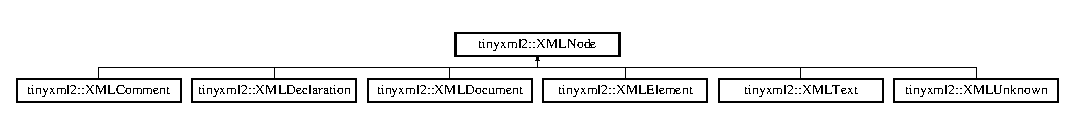
\includegraphics[height=1.145194cm]{classtinyxml2_1_1_x_m_l_node}
\end{center}
\end{figure}
\subsection*{Public Member Functions}
\begin{DoxyCompactItemize}
\item 
\mbox{\Hypertarget{classtinyxml2_1_1_x_m_l_node_a2de84cfa4ec3fe249bad745069d145f1}\label{classtinyxml2_1_1_x_m_l_node_a2de84cfa4ec3fe249bad745069d145f1}} 
const \mbox{\hyperlink{classtinyxml2_1_1_x_m_l_document}{X\+M\+L\+Document}} $\ast$ \mbox{\hyperlink{classtinyxml2_1_1_x_m_l_node_a2de84cfa4ec3fe249bad745069d145f1}{Get\+Document}} () const
\begin{DoxyCompactList}\small\item\em Get the \mbox{\hyperlink{classtinyxml2_1_1_x_m_l_document}{X\+M\+L\+Document}} that owns this \mbox{\hyperlink{classtinyxml2_1_1_x_m_l_node}{X\+M\+L\+Node}}. \end{DoxyCompactList}\item 
\mbox{\Hypertarget{classtinyxml2_1_1_x_m_l_node_af343d1ef0b45c0020e62d784d7e67a68}\label{classtinyxml2_1_1_x_m_l_node_af343d1ef0b45c0020e62d784d7e67a68}} 
\mbox{\hyperlink{classtinyxml2_1_1_x_m_l_document}{X\+M\+L\+Document}} $\ast$ \mbox{\hyperlink{classtinyxml2_1_1_x_m_l_node_af343d1ef0b45c0020e62d784d7e67a68}{Get\+Document}} ()
\begin{DoxyCompactList}\small\item\em Get the \mbox{\hyperlink{classtinyxml2_1_1_x_m_l_document}{X\+M\+L\+Document}} that owns this \mbox{\hyperlink{classtinyxml2_1_1_x_m_l_node}{X\+M\+L\+Node}}. \end{DoxyCompactList}\item 
\mbox{\Hypertarget{classtinyxml2_1_1_x_m_l_node_aab516e699567f75cc9ab2ef2eee501e8}\label{classtinyxml2_1_1_x_m_l_node_aab516e699567f75cc9ab2ef2eee501e8}} 
virtual \mbox{\hyperlink{classtinyxml2_1_1_x_m_l_element}{X\+M\+L\+Element}} $\ast$ \mbox{\hyperlink{classtinyxml2_1_1_x_m_l_node_aab516e699567f75cc9ab2ef2eee501e8}{To\+Element}} ()
\begin{DoxyCompactList}\small\item\em Safely cast to an Element, or null. \end{DoxyCompactList}\item 
\mbox{\Hypertarget{classtinyxml2_1_1_x_m_l_node_a41c55dab9162d1eb62db2008430e376b}\label{classtinyxml2_1_1_x_m_l_node_a41c55dab9162d1eb62db2008430e376b}} 
virtual \mbox{\hyperlink{classtinyxml2_1_1_x_m_l_text}{X\+M\+L\+Text}} $\ast$ \mbox{\hyperlink{classtinyxml2_1_1_x_m_l_node_a41c55dab9162d1eb62db2008430e376b}{To\+Text}} ()
\begin{DoxyCompactList}\small\item\em Safely cast to Text, or null. \end{DoxyCompactList}\item 
\mbox{\Hypertarget{classtinyxml2_1_1_x_m_l_node_aff47671055aa99840a1c1ebd661e63e3}\label{classtinyxml2_1_1_x_m_l_node_aff47671055aa99840a1c1ebd661e63e3}} 
virtual \mbox{\hyperlink{classtinyxml2_1_1_x_m_l_comment}{X\+M\+L\+Comment}} $\ast$ \mbox{\hyperlink{classtinyxml2_1_1_x_m_l_node_aff47671055aa99840a1c1ebd661e63e3}{To\+Comment}} ()
\begin{DoxyCompactList}\small\item\em Safely cast to a Comment, or null. \end{DoxyCompactList}\item 
\mbox{\Hypertarget{classtinyxml2_1_1_x_m_l_node_a836e2966ed736fc3c94f70e12a2a3357}\label{classtinyxml2_1_1_x_m_l_node_a836e2966ed736fc3c94f70e12a2a3357}} 
virtual \mbox{\hyperlink{classtinyxml2_1_1_x_m_l_document}{X\+M\+L\+Document}} $\ast$ \mbox{\hyperlink{classtinyxml2_1_1_x_m_l_node_a836e2966ed736fc3c94f70e12a2a3357}{To\+Document}} ()
\begin{DoxyCompactList}\small\item\em Safely cast to a Document, or null. \end{DoxyCompactList}\item 
\mbox{\Hypertarget{classtinyxml2_1_1_x_m_l_node_a174fd4c22c010b58138c1b84a0dfbd51}\label{classtinyxml2_1_1_x_m_l_node_a174fd4c22c010b58138c1b84a0dfbd51}} 
virtual \mbox{\hyperlink{classtinyxml2_1_1_x_m_l_declaration}{X\+M\+L\+Declaration}} $\ast$ \mbox{\hyperlink{classtinyxml2_1_1_x_m_l_node_a174fd4c22c010b58138c1b84a0dfbd51}{To\+Declaration}} ()
\begin{DoxyCompactList}\small\item\em Safely cast to a Declaration, or null. \end{DoxyCompactList}\item 
\mbox{\Hypertarget{classtinyxml2_1_1_x_m_l_node_a8675a74aa0ada6eccab0c77ef3e5b9bd}\label{classtinyxml2_1_1_x_m_l_node_a8675a74aa0ada6eccab0c77ef3e5b9bd}} 
virtual \mbox{\hyperlink{classtinyxml2_1_1_x_m_l_unknown}{X\+M\+L\+Unknown}} $\ast$ \mbox{\hyperlink{classtinyxml2_1_1_x_m_l_node_a8675a74aa0ada6eccab0c77ef3e5b9bd}{To\+Unknown}} ()
\begin{DoxyCompactList}\small\item\em Safely cast to an Unknown, or null. \end{DoxyCompactList}\item 
\mbox{\Hypertarget{classtinyxml2_1_1_x_m_l_node_a2c5c843b8f37306f15994ebe882b9346}\label{classtinyxml2_1_1_x_m_l_node_a2c5c843b8f37306f15994ebe882b9346}} 
virtual const \mbox{\hyperlink{classtinyxml2_1_1_x_m_l_element}{X\+M\+L\+Element}} $\ast$ {\bfseries To\+Element} () const
\item 
\mbox{\Hypertarget{classtinyxml2_1_1_x_m_l_node_acb9ccc1beda27c0efcb0545683c3e7f4}\label{classtinyxml2_1_1_x_m_l_node_acb9ccc1beda27c0efcb0545683c3e7f4}} 
virtual const \mbox{\hyperlink{classtinyxml2_1_1_x_m_l_text}{X\+M\+L\+Text}} $\ast$ {\bfseries To\+Text} () const
\item 
\mbox{\Hypertarget{classtinyxml2_1_1_x_m_l_node_a6a53bb83faf5c0ccc95b6cf74dba0025}\label{classtinyxml2_1_1_x_m_l_node_a6a53bb83faf5c0ccc95b6cf74dba0025}} 
virtual const \mbox{\hyperlink{classtinyxml2_1_1_x_m_l_comment}{X\+M\+L\+Comment}} $\ast$ {\bfseries To\+Comment} () const
\item 
\mbox{\Hypertarget{classtinyxml2_1_1_x_m_l_node_ae8a5250331a5f12e10843fcb5ef3ef0b}\label{classtinyxml2_1_1_x_m_l_node_ae8a5250331a5f12e10843fcb5ef3ef0b}} 
virtual const \mbox{\hyperlink{classtinyxml2_1_1_x_m_l_document}{X\+M\+L\+Document}} $\ast$ {\bfseries To\+Document} () const
\item 
\mbox{\Hypertarget{classtinyxml2_1_1_x_m_l_node_ac48bb4bf9eb7bb3654ad4b94945db9a1}\label{classtinyxml2_1_1_x_m_l_node_ac48bb4bf9eb7bb3654ad4b94945db9a1}} 
virtual const \mbox{\hyperlink{classtinyxml2_1_1_x_m_l_declaration}{X\+M\+L\+Declaration}} $\ast$ {\bfseries To\+Declaration} () const
\item 
\mbox{\Hypertarget{classtinyxml2_1_1_x_m_l_node_af29ffd6cbe609b6fa04a705256150408}\label{classtinyxml2_1_1_x_m_l_node_af29ffd6cbe609b6fa04a705256150408}} 
virtual const \mbox{\hyperlink{classtinyxml2_1_1_x_m_l_unknown}{X\+M\+L\+Unknown}} $\ast$ {\bfseries To\+Unknown} () const
\item 
const char $\ast$ \mbox{\hyperlink{classtinyxml2_1_1_x_m_l_node_a0485e51c670e741884cfd8362274d680}{Value}} () const
\item 
void \mbox{\hyperlink{classtinyxml2_1_1_x_m_l_node_a09dd68cf9eae137579f6e50f36487513}{Set\+Value}} (const char $\ast$val, bool static\+Mem=false)
\item 
\mbox{\Hypertarget{classtinyxml2_1_1_x_m_l_node_a9b5fc636646fda761d342c72e91cb286}\label{classtinyxml2_1_1_x_m_l_node_a9b5fc636646fda761d342c72e91cb286}} 
int \mbox{\hyperlink{classtinyxml2_1_1_x_m_l_node_a9b5fc636646fda761d342c72e91cb286}{Get\+Line\+Num}} () const
\begin{DoxyCompactList}\small\item\em Gets the line number the node is in, if the document was parsed from a file. \end{DoxyCompactList}\item 
\mbox{\Hypertarget{classtinyxml2_1_1_x_m_l_node_ae0f62bc186c56c2e0483ebd52dbfbe34}\label{classtinyxml2_1_1_x_m_l_node_ae0f62bc186c56c2e0483ebd52dbfbe34}} 
const \mbox{\hyperlink{classtinyxml2_1_1_x_m_l_node}{X\+M\+L\+Node}} $\ast$ \mbox{\hyperlink{classtinyxml2_1_1_x_m_l_node_ae0f62bc186c56c2e0483ebd52dbfbe34}{Parent}} () const
\begin{DoxyCompactList}\small\item\em Get the parent of this node on the D\+OM. \end{DoxyCompactList}\item 
\mbox{\Hypertarget{classtinyxml2_1_1_x_m_l_node_a76029693a5a54fbb721a41d7a0ca8a97}\label{classtinyxml2_1_1_x_m_l_node_a76029693a5a54fbb721a41d7a0ca8a97}} 
\mbox{\hyperlink{classtinyxml2_1_1_x_m_l_node}{X\+M\+L\+Node}} $\ast$ {\bfseries Parent} ()
\item 
\mbox{\Hypertarget{classtinyxml2_1_1_x_m_l_node_ac3ab489e6e202a3cd1762d3b332e89d4}\label{classtinyxml2_1_1_x_m_l_node_ac3ab489e6e202a3cd1762d3b332e89d4}} 
bool \mbox{\hyperlink{classtinyxml2_1_1_x_m_l_node_ac3ab489e6e202a3cd1762d3b332e89d4}{No\+Children}} () const
\begin{DoxyCompactList}\small\item\em Returns true if this node has no children. \end{DoxyCompactList}\item 
\mbox{\Hypertarget{classtinyxml2_1_1_x_m_l_node_ae7dc225e1018cdd685f7563593a1fe08}\label{classtinyxml2_1_1_x_m_l_node_ae7dc225e1018cdd685f7563593a1fe08}} 
const \mbox{\hyperlink{classtinyxml2_1_1_x_m_l_node}{X\+M\+L\+Node}} $\ast$ \mbox{\hyperlink{classtinyxml2_1_1_x_m_l_node_ae7dc225e1018cdd685f7563593a1fe08}{First\+Child}} () const
\begin{DoxyCompactList}\small\item\em Get the first child node, or null if none exists. \end{DoxyCompactList}\item 
\mbox{\Hypertarget{classtinyxml2_1_1_x_m_l_node_a2d6c70c475146b48bc93a7fafdeff5e0}\label{classtinyxml2_1_1_x_m_l_node_a2d6c70c475146b48bc93a7fafdeff5e0}} 
\mbox{\hyperlink{classtinyxml2_1_1_x_m_l_node}{X\+M\+L\+Node}} $\ast$ {\bfseries First\+Child} ()
\item 
const \mbox{\hyperlink{classtinyxml2_1_1_x_m_l_element}{X\+M\+L\+Element}} $\ast$ \mbox{\hyperlink{classtinyxml2_1_1_x_m_l_node_a1bec132dcf085284e0a10755f2cf0d57}{First\+Child\+Element}} (const char $\ast$name=0) const
\item 
\mbox{\Hypertarget{classtinyxml2_1_1_x_m_l_node_af1e0e475cc27d5e7eeaf4d732691b741}\label{classtinyxml2_1_1_x_m_l_node_af1e0e475cc27d5e7eeaf4d732691b741}} 
\mbox{\hyperlink{classtinyxml2_1_1_x_m_l_element}{X\+M\+L\+Element}} $\ast$ {\bfseries First\+Child\+Element} (const char $\ast$name=0)
\item 
\mbox{\Hypertarget{classtinyxml2_1_1_x_m_l_node_a9b8583a277e8e26f4cbbb5492786778e}\label{classtinyxml2_1_1_x_m_l_node_a9b8583a277e8e26f4cbbb5492786778e}} 
const \mbox{\hyperlink{classtinyxml2_1_1_x_m_l_node}{X\+M\+L\+Node}} $\ast$ \mbox{\hyperlink{classtinyxml2_1_1_x_m_l_node_a9b8583a277e8e26f4cbbb5492786778e}{Last\+Child}} () const
\begin{DoxyCompactList}\small\item\em Get the last child node, or null if none exists. \end{DoxyCompactList}\item 
\mbox{\Hypertarget{classtinyxml2_1_1_x_m_l_node_ad7552c8cb1dc0cb6f3bdc14a9d115dbf}\label{classtinyxml2_1_1_x_m_l_node_ad7552c8cb1dc0cb6f3bdc14a9d115dbf}} 
\mbox{\hyperlink{classtinyxml2_1_1_x_m_l_node}{X\+M\+L\+Node}} $\ast$ {\bfseries Last\+Child} ()
\item 
const \mbox{\hyperlink{classtinyxml2_1_1_x_m_l_element}{X\+M\+L\+Element}} $\ast$ \mbox{\hyperlink{classtinyxml2_1_1_x_m_l_node_a609e02f02044f39b928d1a3e0de9f532}{Last\+Child\+Element}} (const char $\ast$name=0) const
\item 
\mbox{\Hypertarget{classtinyxml2_1_1_x_m_l_node_a1b77a8194d059665a4412ebfea276878}\label{classtinyxml2_1_1_x_m_l_node_a1b77a8194d059665a4412ebfea276878}} 
\mbox{\hyperlink{classtinyxml2_1_1_x_m_l_element}{X\+M\+L\+Element}} $\ast$ {\bfseries Last\+Child\+Element} (const char $\ast$name=0)
\item 
\mbox{\Hypertarget{classtinyxml2_1_1_x_m_l_node_aac667c513d445f8b783e1e15ef9d3551}\label{classtinyxml2_1_1_x_m_l_node_aac667c513d445f8b783e1e15ef9d3551}} 
const \mbox{\hyperlink{classtinyxml2_1_1_x_m_l_node}{X\+M\+L\+Node}} $\ast$ \mbox{\hyperlink{classtinyxml2_1_1_x_m_l_node_aac667c513d445f8b783e1e15ef9d3551}{Previous\+Sibling}} () const
\begin{DoxyCompactList}\small\item\em Get the previous (left) sibling node of this node. \end{DoxyCompactList}\item 
\mbox{\Hypertarget{classtinyxml2_1_1_x_m_l_node_ae760e5e7e766df1d2cf3bb4a847876d6}\label{classtinyxml2_1_1_x_m_l_node_ae760e5e7e766df1d2cf3bb4a847876d6}} 
\mbox{\hyperlink{classtinyxml2_1_1_x_m_l_node}{X\+M\+L\+Node}} $\ast$ {\bfseries Previous\+Sibling} ()
\item 
\mbox{\Hypertarget{classtinyxml2_1_1_x_m_l_node_a9453cda5e970375a7b1b2099f8a7c40a}\label{classtinyxml2_1_1_x_m_l_node_a9453cda5e970375a7b1b2099f8a7c40a}} 
const \mbox{\hyperlink{classtinyxml2_1_1_x_m_l_element}{X\+M\+L\+Element}} $\ast$ \mbox{\hyperlink{classtinyxml2_1_1_x_m_l_node_a9453cda5e970375a7b1b2099f8a7c40a}{Previous\+Sibling\+Element}} (const char $\ast$name=0) const
\begin{DoxyCompactList}\small\item\em Get the previous (left) sibling element of this node, with an optionally supplied name. \end{DoxyCompactList}\item 
\mbox{\Hypertarget{classtinyxml2_1_1_x_m_l_node_ae4f37eb6cd405bdf1d57caa066e36d87}\label{classtinyxml2_1_1_x_m_l_node_ae4f37eb6cd405bdf1d57caa066e36d87}} 
\mbox{\hyperlink{classtinyxml2_1_1_x_m_l_element}{X\+M\+L\+Element}} $\ast$ {\bfseries Previous\+Sibling\+Element} (const char $\ast$name=0)
\item 
\mbox{\Hypertarget{classtinyxml2_1_1_x_m_l_node_a79db9ef0fe014d27790f2218b87bcbb5}\label{classtinyxml2_1_1_x_m_l_node_a79db9ef0fe014d27790f2218b87bcbb5}} 
const \mbox{\hyperlink{classtinyxml2_1_1_x_m_l_node}{X\+M\+L\+Node}} $\ast$ \mbox{\hyperlink{classtinyxml2_1_1_x_m_l_node_a79db9ef0fe014d27790f2218b87bcbb5}{Next\+Sibling}} () const
\begin{DoxyCompactList}\small\item\em Get the next (right) sibling node of this node. \end{DoxyCompactList}\item 
\mbox{\Hypertarget{classtinyxml2_1_1_x_m_l_node_aeb7d4dfd8fb924ef86e7cb72183acbac}\label{classtinyxml2_1_1_x_m_l_node_aeb7d4dfd8fb924ef86e7cb72183acbac}} 
\mbox{\hyperlink{classtinyxml2_1_1_x_m_l_node}{X\+M\+L\+Node}} $\ast$ {\bfseries Next\+Sibling} ()
\item 
\mbox{\Hypertarget{classtinyxml2_1_1_x_m_l_node_a14ea560df31110ff07a9f566171bf797}\label{classtinyxml2_1_1_x_m_l_node_a14ea560df31110ff07a9f566171bf797}} 
const \mbox{\hyperlink{classtinyxml2_1_1_x_m_l_element}{X\+M\+L\+Element}} $\ast$ \mbox{\hyperlink{classtinyxml2_1_1_x_m_l_node_a14ea560df31110ff07a9f566171bf797}{Next\+Sibling\+Element}} (const char $\ast$name=0) const
\begin{DoxyCompactList}\small\item\em Get the next (right) sibling element of this node, with an optionally supplied name. \end{DoxyCompactList}\item 
\mbox{\Hypertarget{classtinyxml2_1_1_x_m_l_node_af1225412584d4a2126f55e96a12e0ec0}\label{classtinyxml2_1_1_x_m_l_node_af1225412584d4a2126f55e96a12e0ec0}} 
\mbox{\hyperlink{classtinyxml2_1_1_x_m_l_element}{X\+M\+L\+Element}} $\ast$ {\bfseries Next\+Sibling\+Element} (const char $\ast$name=0)
\item 
\mbox{\hyperlink{classtinyxml2_1_1_x_m_l_node}{X\+M\+L\+Node}} $\ast$ \mbox{\hyperlink{classtinyxml2_1_1_x_m_l_node_ae3b422e98914d6002ca99bb1d2837103}{Insert\+End\+Child}} (\mbox{\hyperlink{classtinyxml2_1_1_x_m_l_node}{X\+M\+L\+Node}} $\ast$add\+This)
\item 
\mbox{\Hypertarget{classtinyxml2_1_1_x_m_l_node_a663e3a5a378169fd477378f4d17a7649}\label{classtinyxml2_1_1_x_m_l_node_a663e3a5a378169fd477378f4d17a7649}} 
\mbox{\hyperlink{classtinyxml2_1_1_x_m_l_node}{X\+M\+L\+Node}} $\ast$ {\bfseries Link\+End\+Child} (\mbox{\hyperlink{classtinyxml2_1_1_x_m_l_node}{X\+M\+L\+Node}} $\ast$add\+This)
\item 
\mbox{\hyperlink{classtinyxml2_1_1_x_m_l_node}{X\+M\+L\+Node}} $\ast$ \mbox{\hyperlink{classtinyxml2_1_1_x_m_l_node_ac609a8f3ea949027f439280c640bbaf2}{Insert\+First\+Child}} (\mbox{\hyperlink{classtinyxml2_1_1_x_m_l_node}{X\+M\+L\+Node}} $\ast$add\+This)
\item 
\mbox{\hyperlink{classtinyxml2_1_1_x_m_l_node}{X\+M\+L\+Node}} $\ast$ \mbox{\hyperlink{classtinyxml2_1_1_x_m_l_node_a9275138a1b8dd5d8e2c26789bdc23ac8}{Insert\+After\+Child}} (\mbox{\hyperlink{classtinyxml2_1_1_x_m_l_node}{X\+M\+L\+Node}} $\ast$after\+This, \mbox{\hyperlink{classtinyxml2_1_1_x_m_l_node}{X\+M\+L\+Node}} $\ast$add\+This)
\item 
void \mbox{\hyperlink{classtinyxml2_1_1_x_m_l_node_a0360085cc54df5bff85d5c5da13afdce}{Delete\+Children}} ()
\item 
void \mbox{\hyperlink{classtinyxml2_1_1_x_m_l_node_a363b6edbd6ebd55f8387d2b89f2b0921}{Delete\+Child}} (\mbox{\hyperlink{classtinyxml2_1_1_x_m_l_node}{X\+M\+L\+Node}} $\ast$node)
\item 
virtual \mbox{\hyperlink{classtinyxml2_1_1_x_m_l_node}{X\+M\+L\+Node}} $\ast$ \mbox{\hyperlink{classtinyxml2_1_1_x_m_l_node_a8402cbd3129d20e9e6024bbcc0531283}{Shallow\+Clone}} (\mbox{\hyperlink{classtinyxml2_1_1_x_m_l_document}{X\+M\+L\+Document}} $\ast$document) const =0
\item 
\mbox{\hyperlink{classtinyxml2_1_1_x_m_l_node}{X\+M\+L\+Node}} $\ast$ \mbox{\hyperlink{classtinyxml2_1_1_x_m_l_node_a3bb369fd733f1989b751d99a9417adab}{Deep\+Clone}} (\mbox{\hyperlink{classtinyxml2_1_1_x_m_l_document}{X\+M\+L\+Document}} $\ast$target) const
\item 
virtual bool \mbox{\hyperlink{classtinyxml2_1_1_x_m_l_node_a7ce18b751c3ea09eac292dca264f9226}{Shallow\+Equal}} (const \mbox{\hyperlink{classtinyxml2_1_1_x_m_l_node}{X\+M\+L\+Node}} $\ast$compare) const =0
\item 
virtual bool \mbox{\hyperlink{classtinyxml2_1_1_x_m_l_node_a81e66df0a44c67a7af17f3b77a152785}{Accept}} (\mbox{\hyperlink{classtinyxml2_1_1_x_m_l_visitor}{X\+M\+L\+Visitor}} $\ast$visitor) const =0
\item 
void \mbox{\hyperlink{classtinyxml2_1_1_x_m_l_node_a002978fc889cc011d143185f2377eca2}{Set\+User\+Data}} (void $\ast$user\+Data)
\item 
void $\ast$ \mbox{\hyperlink{classtinyxml2_1_1_x_m_l_node_a7f0687574afa03bc479dc44f29db0afe}{Get\+User\+Data}} () const
\end{DoxyCompactItemize}
\subsection*{Protected Member Functions}
\begin{DoxyCompactItemize}
\item 
\mbox{\Hypertarget{classtinyxml2_1_1_x_m_l_node_a29868df6ca383d574f584dfdd15105b6}\label{classtinyxml2_1_1_x_m_l_node_a29868df6ca383d574f584dfdd15105b6}} 
{\bfseries X\+M\+L\+Node} (\mbox{\hyperlink{classtinyxml2_1_1_x_m_l_document}{X\+M\+L\+Document}} $\ast$)
\item 
\mbox{\Hypertarget{classtinyxml2_1_1_x_m_l_node_a916e498914baecbc9a1f012352ef7c69}\label{classtinyxml2_1_1_x_m_l_node_a916e498914baecbc9a1f012352ef7c69}} 
virtual char $\ast$ {\bfseries Parse\+Deep} (char $\ast$p, \mbox{\hyperlink{classtinyxml2_1_1_str_pair}{Str\+Pair}} $\ast$parent\+End\+Tag, int $\ast$cur\+Line\+Num\+Ptr)
\end{DoxyCompactItemize}
\subsection*{Protected Attributes}
\begin{DoxyCompactItemize}
\item 
\mbox{\Hypertarget{classtinyxml2_1_1_x_m_l_node_a8d2d2be0bb6797625551eb0e91f0ff62}\label{classtinyxml2_1_1_x_m_l_node_a8d2d2be0bb6797625551eb0e91f0ff62}} 
\mbox{\hyperlink{classtinyxml2_1_1_x_m_l_document}{X\+M\+L\+Document}} $\ast$ {\bfseries \+\_\+document}
\item 
\mbox{\Hypertarget{classtinyxml2_1_1_x_m_l_node_a176dd1c4965c21c366de192164aa2c13}\label{classtinyxml2_1_1_x_m_l_node_a176dd1c4965c21c366de192164aa2c13}} 
\mbox{\hyperlink{classtinyxml2_1_1_x_m_l_node}{X\+M\+L\+Node}} $\ast$ {\bfseries \+\_\+parent}
\item 
\mbox{\Hypertarget{classtinyxml2_1_1_x_m_l_node_a3ea9884098b8379de2bb5ab3fc85c0fc}\label{classtinyxml2_1_1_x_m_l_node_a3ea9884098b8379de2bb5ab3fc85c0fc}} 
\mbox{\hyperlink{classtinyxml2_1_1_str_pair}{Str\+Pair}} {\bfseries \+\_\+value}
\item 
\mbox{\Hypertarget{classtinyxml2_1_1_x_m_l_node_ab336ed023e15be202ff3b410be01b804}\label{classtinyxml2_1_1_x_m_l_node_ab336ed023e15be202ff3b410be01b804}} 
int {\bfseries \+\_\+parse\+Line\+Num}
\item 
\mbox{\Hypertarget{classtinyxml2_1_1_x_m_l_node_aa20c91e4213dc930c5bdf420322ca342}\label{classtinyxml2_1_1_x_m_l_node_aa20c91e4213dc930c5bdf420322ca342}} 
\mbox{\hyperlink{classtinyxml2_1_1_x_m_l_node}{X\+M\+L\+Node}} $\ast$ {\bfseries \+\_\+first\+Child}
\item 
\mbox{\Hypertarget{classtinyxml2_1_1_x_m_l_node_a099b6560ae44ab9edb8453aaf1a3747b}\label{classtinyxml2_1_1_x_m_l_node_a099b6560ae44ab9edb8453aaf1a3747b}} 
\mbox{\hyperlink{classtinyxml2_1_1_x_m_l_node}{X\+M\+L\+Node}} $\ast$ {\bfseries \+\_\+last\+Child}
\item 
\mbox{\Hypertarget{classtinyxml2_1_1_x_m_l_node_a9739eb0fb9a1188266052055e7a6bf6b}\label{classtinyxml2_1_1_x_m_l_node_a9739eb0fb9a1188266052055e7a6bf6b}} 
\mbox{\hyperlink{classtinyxml2_1_1_x_m_l_node}{X\+M\+L\+Node}} $\ast$ {\bfseries \+\_\+prev}
\item 
\mbox{\Hypertarget{classtinyxml2_1_1_x_m_l_node_a27e985496b37dd00eb5b9cf59b9e3fb1}\label{classtinyxml2_1_1_x_m_l_node_a27e985496b37dd00eb5b9cf59b9e3fb1}} 
\mbox{\hyperlink{classtinyxml2_1_1_x_m_l_node}{X\+M\+L\+Node}} $\ast$ {\bfseries \+\_\+next}
\item 
\mbox{\Hypertarget{classtinyxml2_1_1_x_m_l_node_ac2d5cc463a6c95ec5907d57a119c56da}\label{classtinyxml2_1_1_x_m_l_node_ac2d5cc463a6c95ec5907d57a119c56da}} 
void $\ast$ {\bfseries \+\_\+user\+Data}
\end{DoxyCompactItemize}
\subsection*{Friends}
\begin{DoxyCompactItemize}
\item 
\mbox{\Hypertarget{classtinyxml2_1_1_x_m_l_node_a4eee3bda60c60a30e4e8cd4ea91c4c6e}\label{classtinyxml2_1_1_x_m_l_node_a4eee3bda60c60a30e4e8cd4ea91c4c6e}} 
class {\bfseries X\+M\+L\+Document}
\item 
\mbox{\Hypertarget{classtinyxml2_1_1_x_m_l_node_ac2fba9b6e452829dd892f7392c24e0eb}\label{classtinyxml2_1_1_x_m_l_node_ac2fba9b6e452829dd892f7392c24e0eb}} 
class {\bfseries X\+M\+L\+Element}
\end{DoxyCompactItemize}


\subsection{Detailed Description}
\mbox{\hyperlink{classtinyxml2_1_1_x_m_l_node}{X\+M\+L\+Node}} is a base class for every object that is in the X\+ML Document Object Model (D\+OM), except X\+M\+L\+Attributes. Nodes have siblings, a parent, and children which can be navigated. A node is always in a \mbox{\hyperlink{classtinyxml2_1_1_x_m_l_document}{X\+M\+L\+Document}}. The type of a \mbox{\hyperlink{classtinyxml2_1_1_x_m_l_node}{X\+M\+L\+Node}} can be queried, and it can be cast to its more defined type.

A \mbox{\hyperlink{classtinyxml2_1_1_x_m_l_document}{X\+M\+L\+Document}} allocates memory for all its Nodes. When the \mbox{\hyperlink{classtinyxml2_1_1_x_m_l_document}{X\+M\+L\+Document}} gets deleted, all its Nodes will also be deleted.

\begin{DoxyVerb}A Document can contain: Element (container or leaf)
                        Comment (leaf)
                        Unknown (leaf)
                        Declaration( leaf )

An Element can contain: Element (container or leaf)
                        Text    (leaf)
                        Attributes (not on tree)
                        Comment (leaf)
                        Unknown (leaf)\end{DoxyVerb}
 

\subsection{Member Function Documentation}
\mbox{\Hypertarget{classtinyxml2_1_1_x_m_l_node_a81e66df0a44c67a7af17f3b77a152785}\label{classtinyxml2_1_1_x_m_l_node_a81e66df0a44c67a7af17f3b77a152785}} 
\index{tinyxml2\+::\+X\+M\+L\+Node@{tinyxml2\+::\+X\+M\+L\+Node}!Accept@{Accept}}
\index{Accept@{Accept}!tinyxml2\+::\+X\+M\+L\+Node@{tinyxml2\+::\+X\+M\+L\+Node}}
\subsubsection{\texorpdfstring{Accept()}{Accept()}}
{\footnotesize\ttfamily virtual bool tinyxml2\+::\+X\+M\+L\+Node\+::\+Accept (\begin{DoxyParamCaption}\item[{\mbox{\hyperlink{classtinyxml2_1_1_x_m_l_visitor}{X\+M\+L\+Visitor}} $\ast$}]{visitor }\end{DoxyParamCaption}) const\hspace{0.3cm}{\ttfamily [pure virtual]}}

Accept a hierarchical visit of the nodes in the Tiny\+X\+M\+L-\/2 D\+OM. Every node in the X\+ML tree will be conditionally visited and the host will be called back via the \mbox{\hyperlink{classtinyxml2_1_1_x_m_l_visitor}{X\+M\+L\+Visitor}} interface.

This is essentially a S\+AX interface for Tiny\+X\+M\+L-\/2. (Note however it doesn\textquotesingle{}t re-\/parse the X\+ML for the callbacks, so the performance of Tiny\+X\+M\+L-\/2 is unchanged by using this interface versus any other.)

The interface has been based on ideas from\+:


\begin{DoxyItemize}
\item \href{http://www.saxproject.org/}{\tt http\+://www.\+saxproject.\+org/}
\item \href{http://c2.com/cgi/wiki?HierarchicalVisitorPattern}{\tt http\+://c2.\+com/cgi/wiki?\+Hierarchical\+Visitor\+Pattern}
\end{DoxyItemize}

Which are both good references for \char`\"{}visiting\char`\"{}.

An example of using \mbox{\hyperlink{classtinyxml2_1_1_x_m_l_node_a81e66df0a44c67a7af17f3b77a152785}{Accept()}}\+: \begin{DoxyVerb}XMLPrinter printer;
tinyxmlDoc.Accept( &printer );
const char* xmlcstr = printer.CStr();
\end{DoxyVerb}
 

Implemented in \mbox{\hyperlink{classtinyxml2_1_1_x_m_l_document_ab7be651917a35ab1ff0e4e6d4e565cdf}{tinyxml2\+::\+X\+M\+L\+Document}}, \mbox{\hyperlink{classtinyxml2_1_1_x_m_l_element_a9b2119831e8b85827d5d3e5076788e4a}{tinyxml2\+::\+X\+M\+L\+Element}}, \mbox{\hyperlink{classtinyxml2_1_1_x_m_l_unknown_a8a06b8c82117ca969a432e17a46830fc}{tinyxml2\+::\+X\+M\+L\+Unknown}}, \mbox{\hyperlink{classtinyxml2_1_1_x_m_l_declaration_acf47629d9fc08ed6f1c164a97bcf794b}{tinyxml2\+::\+X\+M\+L\+Declaration}}, \mbox{\hyperlink{classtinyxml2_1_1_x_m_l_comment_a27b37d16cea01b5329dfbbb4f9508e39}{tinyxml2\+::\+X\+M\+L\+Comment}}, and \mbox{\hyperlink{classtinyxml2_1_1_x_m_l_text_a537c60d7e18fb59c45ac2737a29ac47a}{tinyxml2\+::\+X\+M\+L\+Text}}.

\mbox{\Hypertarget{classtinyxml2_1_1_x_m_l_node_a3bb369fd733f1989b751d99a9417adab}\label{classtinyxml2_1_1_x_m_l_node_a3bb369fd733f1989b751d99a9417adab}} 
\index{tinyxml2\+::\+X\+M\+L\+Node@{tinyxml2\+::\+X\+M\+L\+Node}!Deep\+Clone@{Deep\+Clone}}
\index{Deep\+Clone@{Deep\+Clone}!tinyxml2\+::\+X\+M\+L\+Node@{tinyxml2\+::\+X\+M\+L\+Node}}
\subsubsection{\texorpdfstring{Deep\+Clone()}{DeepClone()}}
{\footnotesize\ttfamily \mbox{\hyperlink{classtinyxml2_1_1_x_m_l_node}{X\+M\+L\+Node}} $\ast$ tinyxml2\+::\+X\+M\+L\+Node\+::\+Deep\+Clone (\begin{DoxyParamCaption}\item[{\mbox{\hyperlink{classtinyxml2_1_1_x_m_l_document}{X\+M\+L\+Document}} $\ast$}]{target }\end{DoxyParamCaption}) const}

Make a copy of this node and all its children.

If the \textquotesingle{}target\textquotesingle{} is null, then the nodes will be allocated in the current document. If \textquotesingle{}target\textquotesingle{} is specified, the memory will be allocated is the specified \mbox{\hyperlink{classtinyxml2_1_1_x_m_l_document}{X\+M\+L\+Document}}.

N\+O\+TE\+: This is probably not the correct tool to copy a document, since X\+M\+L\+Documents can have multiple top level X\+M\+L\+Nodes. You probably want to use \mbox{\hyperlink{classtinyxml2_1_1_x_m_l_document_af592ffc91514e25a39664521ac83db45}{X\+M\+L\+Document\+::\+Deep\+Copy()}} \mbox{\Hypertarget{classtinyxml2_1_1_x_m_l_node_a363b6edbd6ebd55f8387d2b89f2b0921}\label{classtinyxml2_1_1_x_m_l_node_a363b6edbd6ebd55f8387d2b89f2b0921}} 
\index{tinyxml2\+::\+X\+M\+L\+Node@{tinyxml2\+::\+X\+M\+L\+Node}!Delete\+Child@{Delete\+Child}}
\index{Delete\+Child@{Delete\+Child}!tinyxml2\+::\+X\+M\+L\+Node@{tinyxml2\+::\+X\+M\+L\+Node}}
\subsubsection{\texorpdfstring{Delete\+Child()}{DeleteChild()}}
{\footnotesize\ttfamily void tinyxml2\+::\+X\+M\+L\+Node\+::\+Delete\+Child (\begin{DoxyParamCaption}\item[{\mbox{\hyperlink{classtinyxml2_1_1_x_m_l_node}{X\+M\+L\+Node}} $\ast$}]{node }\end{DoxyParamCaption})}

Delete a child of this node. \mbox{\Hypertarget{classtinyxml2_1_1_x_m_l_node_a0360085cc54df5bff85d5c5da13afdce}\label{classtinyxml2_1_1_x_m_l_node_a0360085cc54df5bff85d5c5da13afdce}} 
\index{tinyxml2\+::\+X\+M\+L\+Node@{tinyxml2\+::\+X\+M\+L\+Node}!Delete\+Children@{Delete\+Children}}
\index{Delete\+Children@{Delete\+Children}!tinyxml2\+::\+X\+M\+L\+Node@{tinyxml2\+::\+X\+M\+L\+Node}}
\subsubsection{\texorpdfstring{Delete\+Children()}{DeleteChildren()}}
{\footnotesize\ttfamily void tinyxml2\+::\+X\+M\+L\+Node\+::\+Delete\+Children (\begin{DoxyParamCaption}{ }\end{DoxyParamCaption})}

Delete all the children of this node. \mbox{\Hypertarget{classtinyxml2_1_1_x_m_l_node_a1bec132dcf085284e0a10755f2cf0d57}\label{classtinyxml2_1_1_x_m_l_node_a1bec132dcf085284e0a10755f2cf0d57}} 
\index{tinyxml2\+::\+X\+M\+L\+Node@{tinyxml2\+::\+X\+M\+L\+Node}!First\+Child\+Element@{First\+Child\+Element}}
\index{First\+Child\+Element@{First\+Child\+Element}!tinyxml2\+::\+X\+M\+L\+Node@{tinyxml2\+::\+X\+M\+L\+Node}}
\subsubsection{\texorpdfstring{First\+Child\+Element()}{FirstChildElement()}}
{\footnotesize\ttfamily const \mbox{\hyperlink{classtinyxml2_1_1_x_m_l_element}{X\+M\+L\+Element}} $\ast$ tinyxml2\+::\+X\+M\+L\+Node\+::\+First\+Child\+Element (\begin{DoxyParamCaption}\item[{const char $\ast$}]{name = {\ttfamily 0} }\end{DoxyParamCaption}) const}

Get the first child element, or optionally the first child element with the specified name. \mbox{\Hypertarget{classtinyxml2_1_1_x_m_l_node_a7f0687574afa03bc479dc44f29db0afe}\label{classtinyxml2_1_1_x_m_l_node_a7f0687574afa03bc479dc44f29db0afe}} 
\index{tinyxml2\+::\+X\+M\+L\+Node@{tinyxml2\+::\+X\+M\+L\+Node}!Get\+User\+Data@{Get\+User\+Data}}
\index{Get\+User\+Data@{Get\+User\+Data}!tinyxml2\+::\+X\+M\+L\+Node@{tinyxml2\+::\+X\+M\+L\+Node}}
\subsubsection{\texorpdfstring{Get\+User\+Data()}{GetUserData()}}
{\footnotesize\ttfamily void$\ast$ tinyxml2\+::\+X\+M\+L\+Node\+::\+Get\+User\+Data (\begin{DoxyParamCaption}{ }\end{DoxyParamCaption}) const\hspace{0.3cm}{\ttfamily [inline]}}

Get user data set into the \mbox{\hyperlink{classtinyxml2_1_1_x_m_l_node}{X\+M\+L\+Node}}. Tiny\+X\+M\+L-\/2 in no way processes or interprets user data. It is initially 0. \mbox{\Hypertarget{classtinyxml2_1_1_x_m_l_node_a9275138a1b8dd5d8e2c26789bdc23ac8}\label{classtinyxml2_1_1_x_m_l_node_a9275138a1b8dd5d8e2c26789bdc23ac8}} 
\index{tinyxml2\+::\+X\+M\+L\+Node@{tinyxml2\+::\+X\+M\+L\+Node}!Insert\+After\+Child@{Insert\+After\+Child}}
\index{Insert\+After\+Child@{Insert\+After\+Child}!tinyxml2\+::\+X\+M\+L\+Node@{tinyxml2\+::\+X\+M\+L\+Node}}
\subsubsection{\texorpdfstring{Insert\+After\+Child()}{InsertAfterChild()}}
{\footnotesize\ttfamily \mbox{\hyperlink{classtinyxml2_1_1_x_m_l_node}{X\+M\+L\+Node}} $\ast$ tinyxml2\+::\+X\+M\+L\+Node\+::\+Insert\+After\+Child (\begin{DoxyParamCaption}\item[{\mbox{\hyperlink{classtinyxml2_1_1_x_m_l_node}{X\+M\+L\+Node}} $\ast$}]{after\+This,  }\item[{\mbox{\hyperlink{classtinyxml2_1_1_x_m_l_node}{X\+M\+L\+Node}} $\ast$}]{add\+This }\end{DoxyParamCaption})}

Add a node after the specified child node. If the child node is already part of the document, it is moved from its old location to the new location. Returns the add\+This argument or 0 if the after\+This node is not a child of this node, or if the node does not belong to the same document. \mbox{\Hypertarget{classtinyxml2_1_1_x_m_l_node_ae3b422e98914d6002ca99bb1d2837103}\label{classtinyxml2_1_1_x_m_l_node_ae3b422e98914d6002ca99bb1d2837103}} 
\index{tinyxml2\+::\+X\+M\+L\+Node@{tinyxml2\+::\+X\+M\+L\+Node}!Insert\+End\+Child@{Insert\+End\+Child}}
\index{Insert\+End\+Child@{Insert\+End\+Child}!tinyxml2\+::\+X\+M\+L\+Node@{tinyxml2\+::\+X\+M\+L\+Node}}
\subsubsection{\texorpdfstring{Insert\+End\+Child()}{InsertEndChild()}}
{\footnotesize\ttfamily \mbox{\hyperlink{classtinyxml2_1_1_x_m_l_node}{X\+M\+L\+Node}} $\ast$ tinyxml2\+::\+X\+M\+L\+Node\+::\+Insert\+End\+Child (\begin{DoxyParamCaption}\item[{\mbox{\hyperlink{classtinyxml2_1_1_x_m_l_node}{X\+M\+L\+Node}} $\ast$}]{add\+This }\end{DoxyParamCaption})}

Add a child node as the last (right) child. If the child node is already part of the document, it is moved from its old location to the new location. Returns the add\+This argument or 0 if the node does not belong to the same document. \mbox{\Hypertarget{classtinyxml2_1_1_x_m_l_node_ac609a8f3ea949027f439280c640bbaf2}\label{classtinyxml2_1_1_x_m_l_node_ac609a8f3ea949027f439280c640bbaf2}} 
\index{tinyxml2\+::\+X\+M\+L\+Node@{tinyxml2\+::\+X\+M\+L\+Node}!Insert\+First\+Child@{Insert\+First\+Child}}
\index{Insert\+First\+Child@{Insert\+First\+Child}!tinyxml2\+::\+X\+M\+L\+Node@{tinyxml2\+::\+X\+M\+L\+Node}}
\subsubsection{\texorpdfstring{Insert\+First\+Child()}{InsertFirstChild()}}
{\footnotesize\ttfamily \mbox{\hyperlink{classtinyxml2_1_1_x_m_l_node}{X\+M\+L\+Node}} $\ast$ tinyxml2\+::\+X\+M\+L\+Node\+::\+Insert\+First\+Child (\begin{DoxyParamCaption}\item[{\mbox{\hyperlink{classtinyxml2_1_1_x_m_l_node}{X\+M\+L\+Node}} $\ast$}]{add\+This }\end{DoxyParamCaption})}

Add a child node as the first (left) child. If the child node is already part of the document, it is moved from its old location to the new location. Returns the add\+This argument or 0 if the node does not belong to the same document. \mbox{\Hypertarget{classtinyxml2_1_1_x_m_l_node_a609e02f02044f39b928d1a3e0de9f532}\label{classtinyxml2_1_1_x_m_l_node_a609e02f02044f39b928d1a3e0de9f532}} 
\index{tinyxml2\+::\+X\+M\+L\+Node@{tinyxml2\+::\+X\+M\+L\+Node}!Last\+Child\+Element@{Last\+Child\+Element}}
\index{Last\+Child\+Element@{Last\+Child\+Element}!tinyxml2\+::\+X\+M\+L\+Node@{tinyxml2\+::\+X\+M\+L\+Node}}
\subsubsection{\texorpdfstring{Last\+Child\+Element()}{LastChildElement()}}
{\footnotesize\ttfamily const \mbox{\hyperlink{classtinyxml2_1_1_x_m_l_element}{X\+M\+L\+Element}} $\ast$ tinyxml2\+::\+X\+M\+L\+Node\+::\+Last\+Child\+Element (\begin{DoxyParamCaption}\item[{const char $\ast$}]{name = {\ttfamily 0} }\end{DoxyParamCaption}) const}

Get the last child element or optionally the last child element with the specified name. \mbox{\Hypertarget{classtinyxml2_1_1_x_m_l_node_a002978fc889cc011d143185f2377eca2}\label{classtinyxml2_1_1_x_m_l_node_a002978fc889cc011d143185f2377eca2}} 
\index{tinyxml2\+::\+X\+M\+L\+Node@{tinyxml2\+::\+X\+M\+L\+Node}!Set\+User\+Data@{Set\+User\+Data}}
\index{Set\+User\+Data@{Set\+User\+Data}!tinyxml2\+::\+X\+M\+L\+Node@{tinyxml2\+::\+X\+M\+L\+Node}}
\subsubsection{\texorpdfstring{Set\+User\+Data()}{SetUserData()}}
{\footnotesize\ttfamily void tinyxml2\+::\+X\+M\+L\+Node\+::\+Set\+User\+Data (\begin{DoxyParamCaption}\item[{void $\ast$}]{user\+Data }\end{DoxyParamCaption})\hspace{0.3cm}{\ttfamily [inline]}}

Set user data into the \mbox{\hyperlink{classtinyxml2_1_1_x_m_l_node}{X\+M\+L\+Node}}. Tiny\+X\+M\+L-\/2 in no way processes or interprets user data. It is initially 0. \mbox{\Hypertarget{classtinyxml2_1_1_x_m_l_node_a09dd68cf9eae137579f6e50f36487513}\label{classtinyxml2_1_1_x_m_l_node_a09dd68cf9eae137579f6e50f36487513}} 
\index{tinyxml2\+::\+X\+M\+L\+Node@{tinyxml2\+::\+X\+M\+L\+Node}!Set\+Value@{Set\+Value}}
\index{Set\+Value@{Set\+Value}!tinyxml2\+::\+X\+M\+L\+Node@{tinyxml2\+::\+X\+M\+L\+Node}}
\subsubsection{\texorpdfstring{Set\+Value()}{SetValue()}}
{\footnotesize\ttfamily void tinyxml2\+::\+X\+M\+L\+Node\+::\+Set\+Value (\begin{DoxyParamCaption}\item[{const char $\ast$}]{val,  }\item[{bool}]{static\+Mem = {\ttfamily false} }\end{DoxyParamCaption})}

Set the Value of an X\+ML node. \begin{DoxySeeAlso}{See also}
\mbox{\hyperlink{classtinyxml2_1_1_x_m_l_node_a0485e51c670e741884cfd8362274d680}{Value()}} 
\end{DoxySeeAlso}
\mbox{\Hypertarget{classtinyxml2_1_1_x_m_l_node_a8402cbd3129d20e9e6024bbcc0531283}\label{classtinyxml2_1_1_x_m_l_node_a8402cbd3129d20e9e6024bbcc0531283}} 
\index{tinyxml2\+::\+X\+M\+L\+Node@{tinyxml2\+::\+X\+M\+L\+Node}!Shallow\+Clone@{Shallow\+Clone}}
\index{Shallow\+Clone@{Shallow\+Clone}!tinyxml2\+::\+X\+M\+L\+Node@{tinyxml2\+::\+X\+M\+L\+Node}}
\subsubsection{\texorpdfstring{Shallow\+Clone()}{ShallowClone()}}
{\footnotesize\ttfamily virtual \mbox{\hyperlink{classtinyxml2_1_1_x_m_l_node}{X\+M\+L\+Node}}$\ast$ tinyxml2\+::\+X\+M\+L\+Node\+::\+Shallow\+Clone (\begin{DoxyParamCaption}\item[{\mbox{\hyperlink{classtinyxml2_1_1_x_m_l_document}{X\+M\+L\+Document}} $\ast$}]{document }\end{DoxyParamCaption}) const\hspace{0.3cm}{\ttfamily [pure virtual]}}

Make a copy of this node, but not its children. You may pass in a Document pointer that will be the owner of the new Node. If the \textquotesingle{}document\textquotesingle{} is null, then the node returned will be allocated from the current Document. (this-\/$>$\mbox{\hyperlink{classtinyxml2_1_1_x_m_l_node_af343d1ef0b45c0020e62d784d7e67a68}{Get\+Document()}})

Note\+: if called on a \mbox{\hyperlink{classtinyxml2_1_1_x_m_l_document}{X\+M\+L\+Document}}, this will return null. 

Implemented in \mbox{\hyperlink{classtinyxml2_1_1_x_m_l_document_aa37cc1709d7e1e988bc17dcfb24a69b8}{tinyxml2\+::\+X\+M\+L\+Document}}, \mbox{\hyperlink{classtinyxml2_1_1_x_m_l_element_aafa2807a45b28fe096b29d76e6a13b7c}{tinyxml2\+::\+X\+M\+L\+Element}}, \mbox{\hyperlink{classtinyxml2_1_1_x_m_l_unknown_ab73b48b819aa4b2ef3815dc2d7d20d5f}{tinyxml2\+::\+X\+M\+L\+Unknown}}, \mbox{\hyperlink{classtinyxml2_1_1_x_m_l_declaration_ad9d60e6d2df75c13eb6bf7319985b747}{tinyxml2\+::\+X\+M\+L\+Declaration}}, \mbox{\hyperlink{classtinyxml2_1_1_x_m_l_comment_adf5b5c0319351dcc339df098d11e8fb2}{tinyxml2\+::\+X\+M\+L\+Comment}}, and \mbox{\hyperlink{classtinyxml2_1_1_x_m_l_text_a86d265c93152726c8c6831e9594840e6}{tinyxml2\+::\+X\+M\+L\+Text}}.

\mbox{\Hypertarget{classtinyxml2_1_1_x_m_l_node_a7ce18b751c3ea09eac292dca264f9226}\label{classtinyxml2_1_1_x_m_l_node_a7ce18b751c3ea09eac292dca264f9226}} 
\index{tinyxml2\+::\+X\+M\+L\+Node@{tinyxml2\+::\+X\+M\+L\+Node}!Shallow\+Equal@{Shallow\+Equal}}
\index{Shallow\+Equal@{Shallow\+Equal}!tinyxml2\+::\+X\+M\+L\+Node@{tinyxml2\+::\+X\+M\+L\+Node}}
\subsubsection{\texorpdfstring{Shallow\+Equal()}{ShallowEqual()}}
{\footnotesize\ttfamily virtual bool tinyxml2\+::\+X\+M\+L\+Node\+::\+Shallow\+Equal (\begin{DoxyParamCaption}\item[{const \mbox{\hyperlink{classtinyxml2_1_1_x_m_l_node}{X\+M\+L\+Node}} $\ast$}]{compare }\end{DoxyParamCaption}) const\hspace{0.3cm}{\ttfamily [pure virtual]}}

Test if 2 nodes are the same, but don\textquotesingle{}t test children. The 2 nodes do not need to be in the same Document.

Note\+: if called on a \mbox{\hyperlink{classtinyxml2_1_1_x_m_l_document}{X\+M\+L\+Document}}, this will return false. 

Implemented in \mbox{\hyperlink{classtinyxml2_1_1_x_m_l_document_a6fe5ef18699091844fcf64b56ffa5bf9}{tinyxml2\+::\+X\+M\+L\+Document}}, \mbox{\hyperlink{classtinyxml2_1_1_x_m_l_element_a61ffd7bf918a9db4aa6203d855ac5ec2}{tinyxml2\+::\+X\+M\+L\+Element}}, \mbox{\hyperlink{classtinyxml2_1_1_x_m_l_unknown_ac46767cd721d666e690a6231dfb618d1}{tinyxml2\+::\+X\+M\+L\+Unknown}}, \mbox{\hyperlink{classtinyxml2_1_1_x_m_l_declaration_ae8b4d3a399857029f36c322b0801b69c}{tinyxml2\+::\+X\+M\+L\+Declaration}}, \mbox{\hyperlink{classtinyxml2_1_1_x_m_l_comment_a965d880a99d58dd915caa88dc37a9b51}{tinyxml2\+::\+X\+M\+L\+Comment}}, and \mbox{\hyperlink{classtinyxml2_1_1_x_m_l_text_a99d8bce4dc01df889126e047f358cdfc}{tinyxml2\+::\+X\+M\+L\+Text}}.

\mbox{\Hypertarget{classtinyxml2_1_1_x_m_l_node_a0485e51c670e741884cfd8362274d680}\label{classtinyxml2_1_1_x_m_l_node_a0485e51c670e741884cfd8362274d680}} 
\index{tinyxml2\+::\+X\+M\+L\+Node@{tinyxml2\+::\+X\+M\+L\+Node}!Value@{Value}}
\index{Value@{Value}!tinyxml2\+::\+X\+M\+L\+Node@{tinyxml2\+::\+X\+M\+L\+Node}}
\subsubsection{\texorpdfstring{Value()}{Value()}}
{\footnotesize\ttfamily const char $\ast$ tinyxml2\+::\+X\+M\+L\+Node\+::\+Value (\begin{DoxyParamCaption}{ }\end{DoxyParamCaption}) const}

The meaning of \textquotesingle{}value\textquotesingle{} changes for the specific type. \begin{DoxyVerb}Document:   empty (NULL is returned, not an empty string)
Element:    name of the element
Comment:    the comment text
Unknown:    the tag contents
Text:       the text string
\end{DoxyVerb}
 

The documentation for this class was generated from the following files\+:\begin{DoxyCompactItemize}
\item 
tinyxml2.\+h\item 
tinyxml2.\+cpp\end{DoxyCompactItemize}

\hypertarget{classtinyxml2_1_1_x_m_l_printer}{}\section{tinyxml2\+:\+:X\+M\+L\+Printer Class Reference}
\label{classtinyxml2_1_1_x_m_l_printer}\index{tinyxml2\+::\+X\+M\+L\+Printer@{tinyxml2\+::\+X\+M\+L\+Printer}}


{\ttfamily \#include $<$tinyxml2.\+h$>$}

Inheritance diagram for tinyxml2\+:\+:X\+M\+L\+Printer\+:\begin{figure}[H]
\begin{center}
\leavevmode
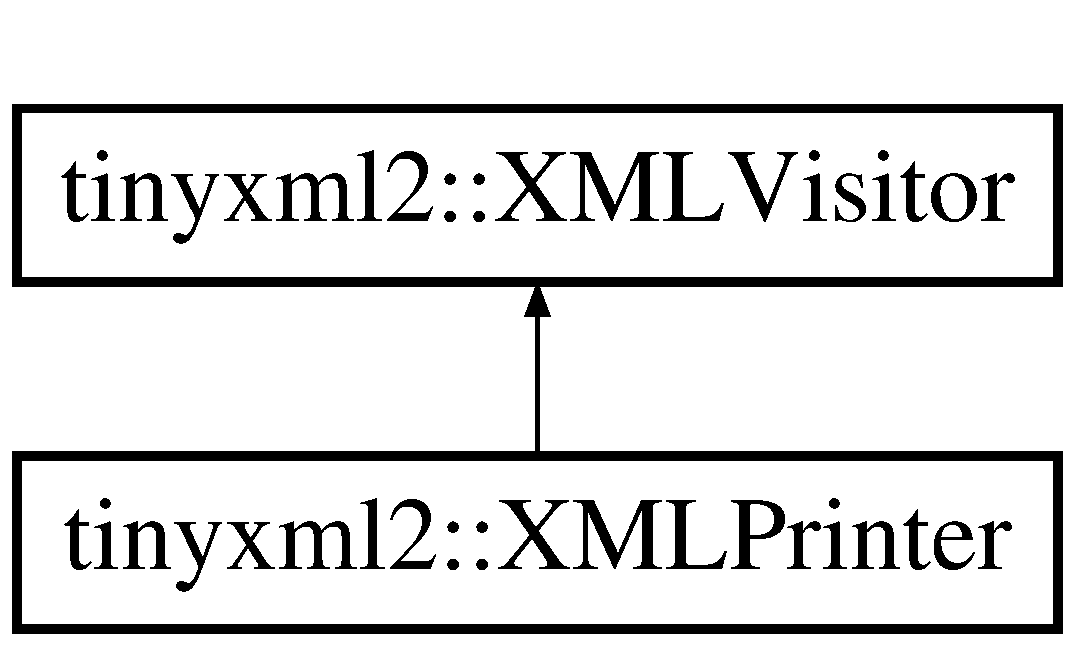
\includegraphics[height=2.000000cm]{classtinyxml2_1_1_x_m_l_printer}
\end{center}
\end{figure}
\subsection*{Public Member Functions}
\begin{DoxyCompactItemize}
\item 
\mbox{\hyperlink{classtinyxml2_1_1_x_m_l_printer_aa6d3841c069085f5b8a27bc7103c04f7}{X\+M\+L\+Printer}} (F\+I\+LE $\ast$file=0, bool compact=false, int depth=0)
\item 
virtual \mbox{\hyperlink{classtinyxml2_1_1_x_m_l_printer_af4caefa48ea6436898fb1807de8d14c0}{$\sim$\+X\+M\+L\+Printer}} ()
\item 
void \mbox{\hyperlink{classtinyxml2_1_1_x_m_l_printer_a178c608ce8476043d5d6513819cde903}{Push\+Header}} (bool write\+B\+OM, bool write\+Declaration)
\item 
void \mbox{\hyperlink{classtinyxml2_1_1_x_m_l_printer_a20fb06c83bd13e5140d7dd13af06c010}{Open\+Element}} (const char $\ast$name, bool compact\+Mode=false)
\item 
void \mbox{\hyperlink{classtinyxml2_1_1_x_m_l_printer_a9a4e2c9348b42e147629d5a99f4af3f0}{Push\+Attribute}} (const char $\ast$name, const char $\ast$value)
\begin{DoxyCompactList}\small\item\em If streaming, add an attribute to an open element. \end{DoxyCompactList}\item 
void \mbox{\hyperlink{classtinyxml2_1_1_x_m_l_printer_a69120c82088597372d28d0a98f2ee7a1}{Push\+Attribute}} (const char $\ast$name, int value)
\item 
void \mbox{\hyperlink{classtinyxml2_1_1_x_m_l_printer_aa41039e51990aaf5342f3e0575a692c4}{Push\+Attribute}} (const char $\ast$name, unsigned value)
\item 
void \mbox{\hyperlink{classtinyxml2_1_1_x_m_l_printer_a9bc2fe21a83a70e6aa0415f2034ecbff}{Push\+Attribute}} (const char $\ast$name, int64\+\_\+t value)
\item 
void \mbox{\hyperlink{classtinyxml2_1_1_x_m_l_printer_a51f7950d7b7a19f0d3a0d549a318d45f}{Push\+Attribute}} (const char $\ast$name, bool value)
\item 
void \mbox{\hyperlink{classtinyxml2_1_1_x_m_l_printer_a1714867af40e68ca404c3e84b6cac2a6}{Push\+Attribute}} (const char $\ast$name, double value)
\item 
virtual void \mbox{\hyperlink{classtinyxml2_1_1_x_m_l_printer_af1fb439e5d800999646f333fa2f0699a}{Close\+Element}} (bool compact\+Mode=false)
\begin{DoxyCompactList}\small\item\em If streaming, close the Element. \end{DoxyCompactList}\item 
void \mbox{\hyperlink{classtinyxml2_1_1_x_m_l_printer_a1cc16a9362df4332012cb13cff6441b3}{Push\+Text}} (const char $\ast$text, bool cdata=false)
\begin{DoxyCompactList}\small\item\em Add a text node. \end{DoxyCompactList}\item 
void \mbox{\hyperlink{classtinyxml2_1_1_x_m_l_printer_a3e0d4d78de25d4cf081009e1431cea7e}{Push\+Text}} (int value)
\begin{DoxyCompactList}\small\item\em Add a text node from an integer. \end{DoxyCompactList}\item 
void \mbox{\hyperlink{classtinyxml2_1_1_x_m_l_printer_a661fb50e7e0a4918d2d259cb0fae647e}{Push\+Text}} (unsigned value)
\begin{DoxyCompactList}\small\item\em Add a text node from an unsigned. \end{DoxyCompactList}\item 
void \mbox{\hyperlink{classtinyxml2_1_1_x_m_l_printer_a96b0a0bfe105154a0a6c37d725258f0a}{Push\+Text}} (int64\+\_\+t value)
\begin{DoxyCompactList}\small\item\em Add a text node from an unsigned. \end{DoxyCompactList}\item 
void \mbox{\hyperlink{classtinyxml2_1_1_x_m_l_printer_a4390e5fa1ed05189a8686647345ab29f}{Push\+Text}} (bool value)
\begin{DoxyCompactList}\small\item\em Add a text node from a bool. \end{DoxyCompactList}\item 
void \mbox{\hyperlink{classtinyxml2_1_1_x_m_l_printer_a1dbb1390e829d0673af66b9cd1928bd7}{Push\+Text}} (float value)
\begin{DoxyCompactList}\small\item\em Add a text node from a float. \end{DoxyCompactList}\item 
void \mbox{\hyperlink{classtinyxml2_1_1_x_m_l_printer_aa715302dfc09473c77c853cbd5431965}{Push\+Text}} (double value)
\begin{DoxyCompactList}\small\item\em Add a text node from a double. \end{DoxyCompactList}\item 
void \mbox{\hyperlink{classtinyxml2_1_1_x_m_l_printer_afc8416814219591c2fd5656e0c233140}{Push\+Comment}} (const char $\ast$comment)
\begin{DoxyCompactList}\small\item\em Add a comment. \end{DoxyCompactList}\item 
void \mbox{\hyperlink{classtinyxml2_1_1_x_m_l_printer_a2fe3565e262594efc6c0276723c83fe7}{Push\+Declaration}} (const char $\ast$value)
\item 
void \mbox{\hyperlink{classtinyxml2_1_1_x_m_l_printer_ab1efc6d1548505e9984185f58f54b713}{Push\+Unknown}} (const char $\ast$value)
\item 
virtual bool \mbox{\hyperlink{classtinyxml2_1_1_x_m_l_printer_a9aa1de11a55a07db55a90fde37d7afad}{Visit\+Enter}} (const \mbox{\hyperlink{classtinyxml2_1_1_x_m_l_document}{X\+M\+L\+Document}} \&)
\begin{DoxyCompactList}\small\item\em Visit a document. \end{DoxyCompactList}\item 
virtual bool \mbox{\hyperlink{classtinyxml2_1_1_x_m_l_printer_a15fc1f2b922f540917dcf52808737b29}{Visit\+Exit}} (const \mbox{\hyperlink{classtinyxml2_1_1_x_m_l_document}{X\+M\+L\+Document}} \&)
\begin{DoxyCompactList}\small\item\em Visit a document. \end{DoxyCompactList}\item 
virtual bool \mbox{\hyperlink{classtinyxml2_1_1_x_m_l_printer_a169b2509d8eabb70811b2bb8cfd1f5d1}{Visit\+Enter}} (const \mbox{\hyperlink{classtinyxml2_1_1_x_m_l_element}{X\+M\+L\+Element}} \&element, const \mbox{\hyperlink{classtinyxml2_1_1_x_m_l_attribute}{X\+M\+L\+Attribute}} $\ast$attribute)
\begin{DoxyCompactList}\small\item\em Visit an element. \end{DoxyCompactList}\item 
virtual bool \mbox{\hyperlink{classtinyxml2_1_1_x_m_l_printer_a2edd48405971a88951c71c9df86a2f50}{Visit\+Exit}} (const \mbox{\hyperlink{classtinyxml2_1_1_x_m_l_element}{X\+M\+L\+Element}} \&element)
\begin{DoxyCompactList}\small\item\em Visit an element. \end{DoxyCompactList}\item 
virtual bool \mbox{\hyperlink{classtinyxml2_1_1_x_m_l_printer_adc0e42b4f6fcb90a95630c79575d030b}{Visit}} (const \mbox{\hyperlink{classtinyxml2_1_1_x_m_l_text}{X\+M\+L\+Text}} \&text)
\begin{DoxyCompactList}\small\item\em Visit a text node. \end{DoxyCompactList}\item 
virtual bool \mbox{\hyperlink{classtinyxml2_1_1_x_m_l_printer_aa294c5c01af0ebb9114902456e4cb53c}{Visit}} (const \mbox{\hyperlink{classtinyxml2_1_1_x_m_l_comment}{X\+M\+L\+Comment}} \&comment)
\begin{DoxyCompactList}\small\item\em Visit a comment node. \end{DoxyCompactList}\item 
virtual bool \mbox{\hyperlink{classtinyxml2_1_1_x_m_l_printer_acfc625b2549304b9c7eb85ebd5c5eb39}{Visit}} (const \mbox{\hyperlink{classtinyxml2_1_1_x_m_l_declaration}{X\+M\+L\+Declaration}} \&declaration)
\begin{DoxyCompactList}\small\item\em Visit a declaration. \end{DoxyCompactList}\item 
virtual bool \mbox{\hyperlink{classtinyxml2_1_1_x_m_l_printer_ab8af5455bbf9e4be2663e6642fcd7e32}{Visit}} (const \mbox{\hyperlink{classtinyxml2_1_1_x_m_l_unknown}{X\+M\+L\+Unknown}} \&unknown)
\begin{DoxyCompactList}\small\item\em Visit an unknown node. \end{DoxyCompactList}\item 
const char $\ast$ \mbox{\hyperlink{classtinyxml2_1_1_x_m_l_printer_a180671d73844f159f2d4aafbc11d106e}{C\+Str}} () const
\item 
int \mbox{\hyperlink{classtinyxml2_1_1_x_m_l_printer_a3256cf3523d4898b91abb18b924be04c}{C\+Str\+Size}} () const
\item 
void \mbox{\hyperlink{classtinyxml2_1_1_x_m_l_printer_a216157765b7267bf389975b1cbf9a909}{Clear\+Buffer}} ()
\end{DoxyCompactItemize}
\subsection*{Protected Member Functions}
\begin{DoxyCompactItemize}
\item 
virtual bool \mbox{\hyperlink{classtinyxml2_1_1_x_m_l_printer_a38e1ed5a779bdf63eda9e808f7a6de66}{Compact\+Mode}} (const \mbox{\hyperlink{classtinyxml2_1_1_x_m_l_element}{X\+M\+L\+Element}} \&)
\item 
virtual void \mbox{\hyperlink{classtinyxml2_1_1_x_m_l_printer_a1c4b2ccbe4fdb316d54f5a93f3559260}{Print\+Space}} (int depth)
\item 
void \mbox{\hyperlink{classtinyxml2_1_1_x_m_l_printer_ab30210a7f32e45634e7a45137bf6fdf6}{Print}} (const char $\ast$format,...)
\item 
void \mbox{\hyperlink{classtinyxml2_1_1_x_m_l_printer_aff363b7634a27538fd691ae62adbda63}{Write}} (const char $\ast$data, size\+\_\+t size)
\item 
void \mbox{\hyperlink{classtinyxml2_1_1_x_m_l_printer_a4bd7f0cabca77ac95c299103fa9592f1}{Write}} (const char $\ast$data)
\item 
void \mbox{\hyperlink{classtinyxml2_1_1_x_m_l_printer_a9567b0218169ba59794f171ae2f9944c}{Putc}} (char ch)
\item 
void \mbox{\hyperlink{classtinyxml2_1_1_x_m_l_printer_ac6e2c72c5d796f5b4de6ce81ca95e3fa}{Seal\+Element\+If\+Just\+Opened}} ()
\end{DoxyCompactItemize}
\subsection*{Protected Attributes}
\begin{DoxyCompactItemize}
\item 
bool \mbox{\hyperlink{classtinyxml2_1_1_x_m_l_printer_ac07169d58b465214a2b1fa306e617c26}{\+\_\+element\+Just\+Opened}}
\item 
\mbox{\hyperlink{classtinyxml2_1_1_dyn_array}{Dyn\+Array}}$<$ const char $\ast$, 10 $>$ \mbox{\hyperlink{classtinyxml2_1_1_x_m_l_printer_a99d59e67e084714541bee3ae43884bef}{\+\_\+stack}}
\end{DoxyCompactItemize}


\subsection{Detailed Description}
Printing functionality. The \mbox{\hyperlink{classtinyxml2_1_1_x_m_l_printer}{X\+M\+L\+Printer}} gives you more options than the \mbox{\hyperlink{classtinyxml2_1_1_x_m_l_document_a867cf5fa3e3ff6ae4847a8b7ee8ec083}{X\+M\+L\+Document\+::\+Print()}} method.

It can\+:
\begin{DoxyEnumerate}
\item Print to memory.
\item Print to a file you provide.
\item Print X\+ML without a \mbox{\hyperlink{classtinyxml2_1_1_x_m_l_document}{X\+M\+L\+Document}}.
\end{DoxyEnumerate}

Print to Memory

\begin{DoxyVerb}XMLPrinter printer;
doc.Print( &printer );
SomeFunction( printer.CStr() );
\end{DoxyVerb}


Print to a File

You provide the file pointer. \begin{DoxyVerb}XMLPrinter printer( fp );
doc.Print( &printer );
\end{DoxyVerb}


Print without a \mbox{\hyperlink{classtinyxml2_1_1_x_m_l_document}{X\+M\+L\+Document}}

When loading, an X\+ML parser is very useful. However, sometimes when saving, it just gets in the way. The code is often set up for streaming, and constructing the D\+OM is just overhead.

The Printer supports the streaming case. The following code prints out a trivially simple X\+ML file without ever creating an X\+ML document.

\begin{DoxyVerb}XMLPrinter printer( fp );
printer.OpenElement( "foo" );
printer.PushAttribute( "foo", "bar" );
printer.CloseElement();
\end{DoxyVerb}
 

\subsection{Constructor \& Destructor Documentation}
\mbox{\Hypertarget{classtinyxml2_1_1_x_m_l_printer_aa6d3841c069085f5b8a27bc7103c04f7}\label{classtinyxml2_1_1_x_m_l_printer_aa6d3841c069085f5b8a27bc7103c04f7}} 
\index{tinyxml2\+::\+X\+M\+L\+Printer@{tinyxml2\+::\+X\+M\+L\+Printer}!X\+M\+L\+Printer@{X\+M\+L\+Printer}}
\index{X\+M\+L\+Printer@{X\+M\+L\+Printer}!tinyxml2\+::\+X\+M\+L\+Printer@{tinyxml2\+::\+X\+M\+L\+Printer}}
\subsubsection{\texorpdfstring{X\+M\+L\+Printer()}{XMLPrinter()}}
{\footnotesize\ttfamily tinyxml2\+::\+X\+M\+L\+Printer\+::\+X\+M\+L\+Printer (\begin{DoxyParamCaption}\item[{F\+I\+LE $\ast$}]{file = {\ttfamily 0},  }\item[{bool}]{compact = {\ttfamily false},  }\item[{int}]{depth = {\ttfamily 0} }\end{DoxyParamCaption})}

Construct the printer. If the F\+I\+L\+E$\ast$ is specified, this will print to the F\+I\+LE. Else it will print to memory, and the result is available in \mbox{\hyperlink{classtinyxml2_1_1_x_m_l_printer_a180671d73844f159f2d4aafbc11d106e}{C\+Str()}}. If \textquotesingle{}compact\textquotesingle{} is set to true, then output is created with only required whitespace and newlines. \mbox{\Hypertarget{classtinyxml2_1_1_x_m_l_printer_af4caefa48ea6436898fb1807de8d14c0}\label{classtinyxml2_1_1_x_m_l_printer_af4caefa48ea6436898fb1807de8d14c0}} 
\index{tinyxml2\+::\+X\+M\+L\+Printer@{tinyxml2\+::\+X\+M\+L\+Printer}!````~X\+M\+L\+Printer@{$\sim$\+X\+M\+L\+Printer}}
\index{````~X\+M\+L\+Printer@{$\sim$\+X\+M\+L\+Printer}!tinyxml2\+::\+X\+M\+L\+Printer@{tinyxml2\+::\+X\+M\+L\+Printer}}
\subsubsection{\texorpdfstring{$\sim$\+X\+M\+L\+Printer()}{~XMLPrinter()}}
{\footnotesize\ttfamily virtual tinyxml2\+::\+X\+M\+L\+Printer\+::$\sim$\+X\+M\+L\+Printer (\begin{DoxyParamCaption}{ }\end{DoxyParamCaption})\hspace{0.3cm}{\ttfamily [inline]}, {\ttfamily [virtual]}}



\subsection{Member Function Documentation}
\mbox{\Hypertarget{classtinyxml2_1_1_x_m_l_printer_a216157765b7267bf389975b1cbf9a909}\label{classtinyxml2_1_1_x_m_l_printer_a216157765b7267bf389975b1cbf9a909}} 
\index{tinyxml2\+::\+X\+M\+L\+Printer@{tinyxml2\+::\+X\+M\+L\+Printer}!Clear\+Buffer@{Clear\+Buffer}}
\index{Clear\+Buffer@{Clear\+Buffer}!tinyxml2\+::\+X\+M\+L\+Printer@{tinyxml2\+::\+X\+M\+L\+Printer}}
\subsubsection{\texorpdfstring{Clear\+Buffer()}{ClearBuffer()}}
{\footnotesize\ttfamily void tinyxml2\+::\+X\+M\+L\+Printer\+::\+Clear\+Buffer (\begin{DoxyParamCaption}{ }\end{DoxyParamCaption})\hspace{0.3cm}{\ttfamily [inline]}}

If in print to memory mode, reset the buffer to the beginning. \mbox{\Hypertarget{classtinyxml2_1_1_x_m_l_printer_af1fb439e5d800999646f333fa2f0699a}\label{classtinyxml2_1_1_x_m_l_printer_af1fb439e5d800999646f333fa2f0699a}} 
\index{tinyxml2\+::\+X\+M\+L\+Printer@{tinyxml2\+::\+X\+M\+L\+Printer}!Close\+Element@{Close\+Element}}
\index{Close\+Element@{Close\+Element}!tinyxml2\+::\+X\+M\+L\+Printer@{tinyxml2\+::\+X\+M\+L\+Printer}}
\subsubsection{\texorpdfstring{Close\+Element()}{CloseElement()}}
{\footnotesize\ttfamily void tinyxml2\+::\+X\+M\+L\+Printer\+::\+Close\+Element (\begin{DoxyParamCaption}\item[{bool}]{compact\+Mode = {\ttfamily false} }\end{DoxyParamCaption})\hspace{0.3cm}{\ttfamily [virtual]}}



If streaming, close the Element. 

\mbox{\Hypertarget{classtinyxml2_1_1_x_m_l_printer_a38e1ed5a779bdf63eda9e808f7a6de66}\label{classtinyxml2_1_1_x_m_l_printer_a38e1ed5a779bdf63eda9e808f7a6de66}} 
\index{tinyxml2\+::\+X\+M\+L\+Printer@{tinyxml2\+::\+X\+M\+L\+Printer}!Compact\+Mode@{Compact\+Mode}}
\index{Compact\+Mode@{Compact\+Mode}!tinyxml2\+::\+X\+M\+L\+Printer@{tinyxml2\+::\+X\+M\+L\+Printer}}
\subsubsection{\texorpdfstring{Compact\+Mode()}{CompactMode()}}
{\footnotesize\ttfamily virtual bool tinyxml2\+::\+X\+M\+L\+Printer\+::\+Compact\+Mode (\begin{DoxyParamCaption}\item[{const \mbox{\hyperlink{classtinyxml2_1_1_x_m_l_element}{X\+M\+L\+Element}} \&}]{ }\end{DoxyParamCaption})\hspace{0.3cm}{\ttfamily [inline]}, {\ttfamily [protected]}, {\ttfamily [virtual]}}

\mbox{\Hypertarget{classtinyxml2_1_1_x_m_l_printer_a180671d73844f159f2d4aafbc11d106e}\label{classtinyxml2_1_1_x_m_l_printer_a180671d73844f159f2d4aafbc11d106e}} 
\index{tinyxml2\+::\+X\+M\+L\+Printer@{tinyxml2\+::\+X\+M\+L\+Printer}!C\+Str@{C\+Str}}
\index{C\+Str@{C\+Str}!tinyxml2\+::\+X\+M\+L\+Printer@{tinyxml2\+::\+X\+M\+L\+Printer}}
\subsubsection{\texorpdfstring{C\+Str()}{CStr()}}
{\footnotesize\ttfamily const char$\ast$ tinyxml2\+::\+X\+M\+L\+Printer\+::\+C\+Str (\begin{DoxyParamCaption}{ }\end{DoxyParamCaption}) const\hspace{0.3cm}{\ttfamily [inline]}}

If in print to memory mode, return a pointer to the X\+ML file in memory. \mbox{\Hypertarget{classtinyxml2_1_1_x_m_l_printer_a3256cf3523d4898b91abb18b924be04c}\label{classtinyxml2_1_1_x_m_l_printer_a3256cf3523d4898b91abb18b924be04c}} 
\index{tinyxml2\+::\+X\+M\+L\+Printer@{tinyxml2\+::\+X\+M\+L\+Printer}!C\+Str\+Size@{C\+Str\+Size}}
\index{C\+Str\+Size@{C\+Str\+Size}!tinyxml2\+::\+X\+M\+L\+Printer@{tinyxml2\+::\+X\+M\+L\+Printer}}
\subsubsection{\texorpdfstring{C\+Str\+Size()}{CStrSize()}}
{\footnotesize\ttfamily int tinyxml2\+::\+X\+M\+L\+Printer\+::\+C\+Str\+Size (\begin{DoxyParamCaption}{ }\end{DoxyParamCaption}) const\hspace{0.3cm}{\ttfamily [inline]}}

If in print to memory mode, return the size of the X\+ML file in memory. (Note the size returned includes the terminating null.) \mbox{\Hypertarget{classtinyxml2_1_1_x_m_l_printer_a20fb06c83bd13e5140d7dd13af06c010}\label{classtinyxml2_1_1_x_m_l_printer_a20fb06c83bd13e5140d7dd13af06c010}} 
\index{tinyxml2\+::\+X\+M\+L\+Printer@{tinyxml2\+::\+X\+M\+L\+Printer}!Open\+Element@{Open\+Element}}
\index{Open\+Element@{Open\+Element}!tinyxml2\+::\+X\+M\+L\+Printer@{tinyxml2\+::\+X\+M\+L\+Printer}}
\subsubsection{\texorpdfstring{Open\+Element()}{OpenElement()}}
{\footnotesize\ttfamily void tinyxml2\+::\+X\+M\+L\+Printer\+::\+Open\+Element (\begin{DoxyParamCaption}\item[{const char $\ast$}]{name,  }\item[{bool}]{compact\+Mode = {\ttfamily false} }\end{DoxyParamCaption})}

If streaming, start writing an element. The element must be closed with \mbox{\hyperlink{classtinyxml2_1_1_x_m_l_printer_af1fb439e5d800999646f333fa2f0699a}{Close\+Element()}} \mbox{\Hypertarget{classtinyxml2_1_1_x_m_l_printer_ab30210a7f32e45634e7a45137bf6fdf6}\label{classtinyxml2_1_1_x_m_l_printer_ab30210a7f32e45634e7a45137bf6fdf6}} 
\index{tinyxml2\+::\+X\+M\+L\+Printer@{tinyxml2\+::\+X\+M\+L\+Printer}!Print@{Print}}
\index{Print@{Print}!tinyxml2\+::\+X\+M\+L\+Printer@{tinyxml2\+::\+X\+M\+L\+Printer}}
\subsubsection{\texorpdfstring{Print()}{Print()}}
{\footnotesize\ttfamily void tinyxml2\+::\+X\+M\+L\+Printer\+::\+Print (\begin{DoxyParamCaption}\item[{const char $\ast$}]{format,  }\item[{}]{... }\end{DoxyParamCaption})\hspace{0.3cm}{\ttfamily [protected]}}

\mbox{\Hypertarget{classtinyxml2_1_1_x_m_l_printer_a1c4b2ccbe4fdb316d54f5a93f3559260}\label{classtinyxml2_1_1_x_m_l_printer_a1c4b2ccbe4fdb316d54f5a93f3559260}} 
\index{tinyxml2\+::\+X\+M\+L\+Printer@{tinyxml2\+::\+X\+M\+L\+Printer}!Print\+Space@{Print\+Space}}
\index{Print\+Space@{Print\+Space}!tinyxml2\+::\+X\+M\+L\+Printer@{tinyxml2\+::\+X\+M\+L\+Printer}}
\subsubsection{\texorpdfstring{Print\+Space()}{PrintSpace()}}
{\footnotesize\ttfamily void tinyxml2\+::\+X\+M\+L\+Printer\+::\+Print\+Space (\begin{DoxyParamCaption}\item[{int}]{depth }\end{DoxyParamCaption})\hspace{0.3cm}{\ttfamily [protected]}, {\ttfamily [virtual]}}

Prints out the space before an element. You may override to change the space and tabs used. A \mbox{\hyperlink{classtinyxml2_1_1_x_m_l_printer_a1c4b2ccbe4fdb316d54f5a93f3559260}{Print\+Space()}} override should call \mbox{\hyperlink{classtinyxml2_1_1_x_m_l_printer_ab30210a7f32e45634e7a45137bf6fdf6}{Print()}}. \mbox{\Hypertarget{classtinyxml2_1_1_x_m_l_printer_a9a4e2c9348b42e147629d5a99f4af3f0}\label{classtinyxml2_1_1_x_m_l_printer_a9a4e2c9348b42e147629d5a99f4af3f0}} 
\index{tinyxml2\+::\+X\+M\+L\+Printer@{tinyxml2\+::\+X\+M\+L\+Printer}!Push\+Attribute@{Push\+Attribute}}
\index{Push\+Attribute@{Push\+Attribute}!tinyxml2\+::\+X\+M\+L\+Printer@{tinyxml2\+::\+X\+M\+L\+Printer}}
\subsubsection{\texorpdfstring{Push\+Attribute()}{PushAttribute()}\hspace{0.1cm}{\footnotesize\ttfamily [1/6]}}
{\footnotesize\ttfamily void tinyxml2\+::\+X\+M\+L\+Printer\+::\+Push\+Attribute (\begin{DoxyParamCaption}\item[{const char $\ast$}]{name,  }\item[{const char $\ast$}]{value }\end{DoxyParamCaption})}



If streaming, add an attribute to an open element. 

\mbox{\Hypertarget{classtinyxml2_1_1_x_m_l_printer_a69120c82088597372d28d0a98f2ee7a1}\label{classtinyxml2_1_1_x_m_l_printer_a69120c82088597372d28d0a98f2ee7a1}} 
\index{tinyxml2\+::\+X\+M\+L\+Printer@{tinyxml2\+::\+X\+M\+L\+Printer}!Push\+Attribute@{Push\+Attribute}}
\index{Push\+Attribute@{Push\+Attribute}!tinyxml2\+::\+X\+M\+L\+Printer@{tinyxml2\+::\+X\+M\+L\+Printer}}
\subsubsection{\texorpdfstring{Push\+Attribute()}{PushAttribute()}\hspace{0.1cm}{\footnotesize\ttfamily [2/6]}}
{\footnotesize\ttfamily void tinyxml2\+::\+X\+M\+L\+Printer\+::\+Push\+Attribute (\begin{DoxyParamCaption}\item[{const char $\ast$}]{name,  }\item[{int}]{value }\end{DoxyParamCaption})}

\mbox{\Hypertarget{classtinyxml2_1_1_x_m_l_printer_aa41039e51990aaf5342f3e0575a692c4}\label{classtinyxml2_1_1_x_m_l_printer_aa41039e51990aaf5342f3e0575a692c4}} 
\index{tinyxml2\+::\+X\+M\+L\+Printer@{tinyxml2\+::\+X\+M\+L\+Printer}!Push\+Attribute@{Push\+Attribute}}
\index{Push\+Attribute@{Push\+Attribute}!tinyxml2\+::\+X\+M\+L\+Printer@{tinyxml2\+::\+X\+M\+L\+Printer}}
\subsubsection{\texorpdfstring{Push\+Attribute()}{PushAttribute()}\hspace{0.1cm}{\footnotesize\ttfamily [3/6]}}
{\footnotesize\ttfamily void tinyxml2\+::\+X\+M\+L\+Printer\+::\+Push\+Attribute (\begin{DoxyParamCaption}\item[{const char $\ast$}]{name,  }\item[{unsigned}]{value }\end{DoxyParamCaption})}

\mbox{\Hypertarget{classtinyxml2_1_1_x_m_l_printer_a9bc2fe21a83a70e6aa0415f2034ecbff}\label{classtinyxml2_1_1_x_m_l_printer_a9bc2fe21a83a70e6aa0415f2034ecbff}} 
\index{tinyxml2\+::\+X\+M\+L\+Printer@{tinyxml2\+::\+X\+M\+L\+Printer}!Push\+Attribute@{Push\+Attribute}}
\index{Push\+Attribute@{Push\+Attribute}!tinyxml2\+::\+X\+M\+L\+Printer@{tinyxml2\+::\+X\+M\+L\+Printer}}
\subsubsection{\texorpdfstring{Push\+Attribute()}{PushAttribute()}\hspace{0.1cm}{\footnotesize\ttfamily [4/6]}}
{\footnotesize\ttfamily void tinyxml2\+::\+X\+M\+L\+Printer\+::\+Push\+Attribute (\begin{DoxyParamCaption}\item[{const char $\ast$}]{name,  }\item[{int64\+\_\+t}]{value }\end{DoxyParamCaption})}

\mbox{\Hypertarget{classtinyxml2_1_1_x_m_l_printer_a51f7950d7b7a19f0d3a0d549a318d45f}\label{classtinyxml2_1_1_x_m_l_printer_a51f7950d7b7a19f0d3a0d549a318d45f}} 
\index{tinyxml2\+::\+X\+M\+L\+Printer@{tinyxml2\+::\+X\+M\+L\+Printer}!Push\+Attribute@{Push\+Attribute}}
\index{Push\+Attribute@{Push\+Attribute}!tinyxml2\+::\+X\+M\+L\+Printer@{tinyxml2\+::\+X\+M\+L\+Printer}}
\subsubsection{\texorpdfstring{Push\+Attribute()}{PushAttribute()}\hspace{0.1cm}{\footnotesize\ttfamily [5/6]}}
{\footnotesize\ttfamily void tinyxml2\+::\+X\+M\+L\+Printer\+::\+Push\+Attribute (\begin{DoxyParamCaption}\item[{const char $\ast$}]{name,  }\item[{bool}]{value }\end{DoxyParamCaption})}

\mbox{\Hypertarget{classtinyxml2_1_1_x_m_l_printer_a1714867af40e68ca404c3e84b6cac2a6}\label{classtinyxml2_1_1_x_m_l_printer_a1714867af40e68ca404c3e84b6cac2a6}} 
\index{tinyxml2\+::\+X\+M\+L\+Printer@{tinyxml2\+::\+X\+M\+L\+Printer}!Push\+Attribute@{Push\+Attribute}}
\index{Push\+Attribute@{Push\+Attribute}!tinyxml2\+::\+X\+M\+L\+Printer@{tinyxml2\+::\+X\+M\+L\+Printer}}
\subsubsection{\texorpdfstring{Push\+Attribute()}{PushAttribute()}\hspace{0.1cm}{\footnotesize\ttfamily [6/6]}}
{\footnotesize\ttfamily void tinyxml2\+::\+X\+M\+L\+Printer\+::\+Push\+Attribute (\begin{DoxyParamCaption}\item[{const char $\ast$}]{name,  }\item[{double}]{value }\end{DoxyParamCaption})}

\mbox{\Hypertarget{classtinyxml2_1_1_x_m_l_printer_afc8416814219591c2fd5656e0c233140}\label{classtinyxml2_1_1_x_m_l_printer_afc8416814219591c2fd5656e0c233140}} 
\index{tinyxml2\+::\+X\+M\+L\+Printer@{tinyxml2\+::\+X\+M\+L\+Printer}!Push\+Comment@{Push\+Comment}}
\index{Push\+Comment@{Push\+Comment}!tinyxml2\+::\+X\+M\+L\+Printer@{tinyxml2\+::\+X\+M\+L\+Printer}}
\subsubsection{\texorpdfstring{Push\+Comment()}{PushComment()}}
{\footnotesize\ttfamily void tinyxml2\+::\+X\+M\+L\+Printer\+::\+Push\+Comment (\begin{DoxyParamCaption}\item[{const char $\ast$}]{comment }\end{DoxyParamCaption})}



Add a comment. 

\mbox{\Hypertarget{classtinyxml2_1_1_x_m_l_printer_a2fe3565e262594efc6c0276723c83fe7}\label{classtinyxml2_1_1_x_m_l_printer_a2fe3565e262594efc6c0276723c83fe7}} 
\index{tinyxml2\+::\+X\+M\+L\+Printer@{tinyxml2\+::\+X\+M\+L\+Printer}!Push\+Declaration@{Push\+Declaration}}
\index{Push\+Declaration@{Push\+Declaration}!tinyxml2\+::\+X\+M\+L\+Printer@{tinyxml2\+::\+X\+M\+L\+Printer}}
\subsubsection{\texorpdfstring{Push\+Declaration()}{PushDeclaration()}}
{\footnotesize\ttfamily void tinyxml2\+::\+X\+M\+L\+Printer\+::\+Push\+Declaration (\begin{DoxyParamCaption}\item[{const char $\ast$}]{value }\end{DoxyParamCaption})}

\mbox{\Hypertarget{classtinyxml2_1_1_x_m_l_printer_a178c608ce8476043d5d6513819cde903}\label{classtinyxml2_1_1_x_m_l_printer_a178c608ce8476043d5d6513819cde903}} 
\index{tinyxml2\+::\+X\+M\+L\+Printer@{tinyxml2\+::\+X\+M\+L\+Printer}!Push\+Header@{Push\+Header}}
\index{Push\+Header@{Push\+Header}!tinyxml2\+::\+X\+M\+L\+Printer@{tinyxml2\+::\+X\+M\+L\+Printer}}
\subsubsection{\texorpdfstring{Push\+Header()}{PushHeader()}}
{\footnotesize\ttfamily void tinyxml2\+::\+X\+M\+L\+Printer\+::\+Push\+Header (\begin{DoxyParamCaption}\item[{bool}]{write\+B\+OM,  }\item[{bool}]{write\+Declaration }\end{DoxyParamCaption})}

If streaming, write the B\+OM and declaration. \mbox{\Hypertarget{classtinyxml2_1_1_x_m_l_printer_a1cc16a9362df4332012cb13cff6441b3}\label{classtinyxml2_1_1_x_m_l_printer_a1cc16a9362df4332012cb13cff6441b3}} 
\index{tinyxml2\+::\+X\+M\+L\+Printer@{tinyxml2\+::\+X\+M\+L\+Printer}!Push\+Text@{Push\+Text}}
\index{Push\+Text@{Push\+Text}!tinyxml2\+::\+X\+M\+L\+Printer@{tinyxml2\+::\+X\+M\+L\+Printer}}
\subsubsection{\texorpdfstring{Push\+Text()}{PushText()}\hspace{0.1cm}{\footnotesize\ttfamily [1/7]}}
{\footnotesize\ttfamily void tinyxml2\+::\+X\+M\+L\+Printer\+::\+Push\+Text (\begin{DoxyParamCaption}\item[{const char $\ast$}]{text,  }\item[{bool}]{cdata = {\ttfamily false} }\end{DoxyParamCaption})}



Add a text node. 

\mbox{\Hypertarget{classtinyxml2_1_1_x_m_l_printer_a3e0d4d78de25d4cf081009e1431cea7e}\label{classtinyxml2_1_1_x_m_l_printer_a3e0d4d78de25d4cf081009e1431cea7e}} 
\index{tinyxml2\+::\+X\+M\+L\+Printer@{tinyxml2\+::\+X\+M\+L\+Printer}!Push\+Text@{Push\+Text}}
\index{Push\+Text@{Push\+Text}!tinyxml2\+::\+X\+M\+L\+Printer@{tinyxml2\+::\+X\+M\+L\+Printer}}
\subsubsection{\texorpdfstring{Push\+Text()}{PushText()}\hspace{0.1cm}{\footnotesize\ttfamily [2/7]}}
{\footnotesize\ttfamily void tinyxml2\+::\+X\+M\+L\+Printer\+::\+Push\+Text (\begin{DoxyParamCaption}\item[{int}]{value }\end{DoxyParamCaption})}



Add a text node from an integer. 

\mbox{\Hypertarget{classtinyxml2_1_1_x_m_l_printer_a661fb50e7e0a4918d2d259cb0fae647e}\label{classtinyxml2_1_1_x_m_l_printer_a661fb50e7e0a4918d2d259cb0fae647e}} 
\index{tinyxml2\+::\+X\+M\+L\+Printer@{tinyxml2\+::\+X\+M\+L\+Printer}!Push\+Text@{Push\+Text}}
\index{Push\+Text@{Push\+Text}!tinyxml2\+::\+X\+M\+L\+Printer@{tinyxml2\+::\+X\+M\+L\+Printer}}
\subsubsection{\texorpdfstring{Push\+Text()}{PushText()}\hspace{0.1cm}{\footnotesize\ttfamily [3/7]}}
{\footnotesize\ttfamily void tinyxml2\+::\+X\+M\+L\+Printer\+::\+Push\+Text (\begin{DoxyParamCaption}\item[{unsigned}]{value }\end{DoxyParamCaption})}



Add a text node from an unsigned. 

\mbox{\Hypertarget{classtinyxml2_1_1_x_m_l_printer_a96b0a0bfe105154a0a6c37d725258f0a}\label{classtinyxml2_1_1_x_m_l_printer_a96b0a0bfe105154a0a6c37d725258f0a}} 
\index{tinyxml2\+::\+X\+M\+L\+Printer@{tinyxml2\+::\+X\+M\+L\+Printer}!Push\+Text@{Push\+Text}}
\index{Push\+Text@{Push\+Text}!tinyxml2\+::\+X\+M\+L\+Printer@{tinyxml2\+::\+X\+M\+L\+Printer}}
\subsubsection{\texorpdfstring{Push\+Text()}{PushText()}\hspace{0.1cm}{\footnotesize\ttfamily [4/7]}}
{\footnotesize\ttfamily void tinyxml2\+::\+X\+M\+L\+Printer\+::\+Push\+Text (\begin{DoxyParamCaption}\item[{int64\+\_\+t}]{value }\end{DoxyParamCaption})}



Add a text node from an unsigned. 

\mbox{\Hypertarget{classtinyxml2_1_1_x_m_l_printer_a4390e5fa1ed05189a8686647345ab29f}\label{classtinyxml2_1_1_x_m_l_printer_a4390e5fa1ed05189a8686647345ab29f}} 
\index{tinyxml2\+::\+X\+M\+L\+Printer@{tinyxml2\+::\+X\+M\+L\+Printer}!Push\+Text@{Push\+Text}}
\index{Push\+Text@{Push\+Text}!tinyxml2\+::\+X\+M\+L\+Printer@{tinyxml2\+::\+X\+M\+L\+Printer}}
\subsubsection{\texorpdfstring{Push\+Text()}{PushText()}\hspace{0.1cm}{\footnotesize\ttfamily [5/7]}}
{\footnotesize\ttfamily void tinyxml2\+::\+X\+M\+L\+Printer\+::\+Push\+Text (\begin{DoxyParamCaption}\item[{bool}]{value }\end{DoxyParamCaption})}



Add a text node from a bool. 

\mbox{\Hypertarget{classtinyxml2_1_1_x_m_l_printer_a1dbb1390e829d0673af66b9cd1928bd7}\label{classtinyxml2_1_1_x_m_l_printer_a1dbb1390e829d0673af66b9cd1928bd7}} 
\index{tinyxml2\+::\+X\+M\+L\+Printer@{tinyxml2\+::\+X\+M\+L\+Printer}!Push\+Text@{Push\+Text}}
\index{Push\+Text@{Push\+Text}!tinyxml2\+::\+X\+M\+L\+Printer@{tinyxml2\+::\+X\+M\+L\+Printer}}
\subsubsection{\texorpdfstring{Push\+Text()}{PushText()}\hspace{0.1cm}{\footnotesize\ttfamily [6/7]}}
{\footnotesize\ttfamily void tinyxml2\+::\+X\+M\+L\+Printer\+::\+Push\+Text (\begin{DoxyParamCaption}\item[{float}]{value }\end{DoxyParamCaption})}



Add a text node from a float. 

\mbox{\Hypertarget{classtinyxml2_1_1_x_m_l_printer_aa715302dfc09473c77c853cbd5431965}\label{classtinyxml2_1_1_x_m_l_printer_aa715302dfc09473c77c853cbd5431965}} 
\index{tinyxml2\+::\+X\+M\+L\+Printer@{tinyxml2\+::\+X\+M\+L\+Printer}!Push\+Text@{Push\+Text}}
\index{Push\+Text@{Push\+Text}!tinyxml2\+::\+X\+M\+L\+Printer@{tinyxml2\+::\+X\+M\+L\+Printer}}
\subsubsection{\texorpdfstring{Push\+Text()}{PushText()}\hspace{0.1cm}{\footnotesize\ttfamily [7/7]}}
{\footnotesize\ttfamily void tinyxml2\+::\+X\+M\+L\+Printer\+::\+Push\+Text (\begin{DoxyParamCaption}\item[{double}]{value }\end{DoxyParamCaption})}



Add a text node from a double. 

\mbox{\Hypertarget{classtinyxml2_1_1_x_m_l_printer_ab1efc6d1548505e9984185f58f54b713}\label{classtinyxml2_1_1_x_m_l_printer_ab1efc6d1548505e9984185f58f54b713}} 
\index{tinyxml2\+::\+X\+M\+L\+Printer@{tinyxml2\+::\+X\+M\+L\+Printer}!Push\+Unknown@{Push\+Unknown}}
\index{Push\+Unknown@{Push\+Unknown}!tinyxml2\+::\+X\+M\+L\+Printer@{tinyxml2\+::\+X\+M\+L\+Printer}}
\subsubsection{\texorpdfstring{Push\+Unknown()}{PushUnknown()}}
{\footnotesize\ttfamily void tinyxml2\+::\+X\+M\+L\+Printer\+::\+Push\+Unknown (\begin{DoxyParamCaption}\item[{const char $\ast$}]{value }\end{DoxyParamCaption})}

\mbox{\Hypertarget{classtinyxml2_1_1_x_m_l_printer_a9567b0218169ba59794f171ae2f9944c}\label{classtinyxml2_1_1_x_m_l_printer_a9567b0218169ba59794f171ae2f9944c}} 
\index{tinyxml2\+::\+X\+M\+L\+Printer@{tinyxml2\+::\+X\+M\+L\+Printer}!Putc@{Putc}}
\index{Putc@{Putc}!tinyxml2\+::\+X\+M\+L\+Printer@{tinyxml2\+::\+X\+M\+L\+Printer}}
\subsubsection{\texorpdfstring{Putc()}{Putc()}}
{\footnotesize\ttfamily void tinyxml2\+::\+X\+M\+L\+Printer\+::\+Putc (\begin{DoxyParamCaption}\item[{char}]{ch }\end{DoxyParamCaption})\hspace{0.3cm}{\ttfamily [protected]}}

\mbox{\Hypertarget{classtinyxml2_1_1_x_m_l_printer_ac6e2c72c5d796f5b4de6ce81ca95e3fa}\label{classtinyxml2_1_1_x_m_l_printer_ac6e2c72c5d796f5b4de6ce81ca95e3fa}} 
\index{tinyxml2\+::\+X\+M\+L\+Printer@{tinyxml2\+::\+X\+M\+L\+Printer}!Seal\+Element\+If\+Just\+Opened@{Seal\+Element\+If\+Just\+Opened}}
\index{Seal\+Element\+If\+Just\+Opened@{Seal\+Element\+If\+Just\+Opened}!tinyxml2\+::\+X\+M\+L\+Printer@{tinyxml2\+::\+X\+M\+L\+Printer}}
\subsubsection{\texorpdfstring{Seal\+Element\+If\+Just\+Opened()}{SealElementIfJustOpened()}}
{\footnotesize\ttfamily void tinyxml2\+::\+X\+M\+L\+Printer\+::\+Seal\+Element\+If\+Just\+Opened (\begin{DoxyParamCaption}{ }\end{DoxyParamCaption})\hspace{0.3cm}{\ttfamily [protected]}}

\mbox{\Hypertarget{classtinyxml2_1_1_x_m_l_printer_adc0e42b4f6fcb90a95630c79575d030b}\label{classtinyxml2_1_1_x_m_l_printer_adc0e42b4f6fcb90a95630c79575d030b}} 
\index{tinyxml2\+::\+X\+M\+L\+Printer@{tinyxml2\+::\+X\+M\+L\+Printer}!Visit@{Visit}}
\index{Visit@{Visit}!tinyxml2\+::\+X\+M\+L\+Printer@{tinyxml2\+::\+X\+M\+L\+Printer}}
\subsubsection{\texorpdfstring{Visit()}{Visit()}\hspace{0.1cm}{\footnotesize\ttfamily [1/4]}}
{\footnotesize\ttfamily bool tinyxml2\+::\+X\+M\+L\+Printer\+::\+Visit (\begin{DoxyParamCaption}\item[{const \mbox{\hyperlink{classtinyxml2_1_1_x_m_l_text}{X\+M\+L\+Text}} \&}]{ }\end{DoxyParamCaption})\hspace{0.3cm}{\ttfamily [virtual]}}



Visit a text node. 



Reimplemented from \mbox{\hyperlink{classtinyxml2_1_1_x_m_l_visitor_af30233565856480ea48b6fa0d6dec65b}{tinyxml2\+::\+X\+M\+L\+Visitor}}.

\mbox{\Hypertarget{classtinyxml2_1_1_x_m_l_printer_aa294c5c01af0ebb9114902456e4cb53c}\label{classtinyxml2_1_1_x_m_l_printer_aa294c5c01af0ebb9114902456e4cb53c}} 
\index{tinyxml2\+::\+X\+M\+L\+Printer@{tinyxml2\+::\+X\+M\+L\+Printer}!Visit@{Visit}}
\index{Visit@{Visit}!tinyxml2\+::\+X\+M\+L\+Printer@{tinyxml2\+::\+X\+M\+L\+Printer}}
\subsubsection{\texorpdfstring{Visit()}{Visit()}\hspace{0.1cm}{\footnotesize\ttfamily [2/4]}}
{\footnotesize\ttfamily bool tinyxml2\+::\+X\+M\+L\+Printer\+::\+Visit (\begin{DoxyParamCaption}\item[{const \mbox{\hyperlink{classtinyxml2_1_1_x_m_l_comment}{X\+M\+L\+Comment}} \&}]{ }\end{DoxyParamCaption})\hspace{0.3cm}{\ttfamily [virtual]}}



Visit a comment node. 



Reimplemented from \mbox{\hyperlink{classtinyxml2_1_1_x_m_l_visitor_acc8147fb5a85f6c65721654e427752d7}{tinyxml2\+::\+X\+M\+L\+Visitor}}.

\mbox{\Hypertarget{classtinyxml2_1_1_x_m_l_printer_acfc625b2549304b9c7eb85ebd5c5eb39}\label{classtinyxml2_1_1_x_m_l_printer_acfc625b2549304b9c7eb85ebd5c5eb39}} 
\index{tinyxml2\+::\+X\+M\+L\+Printer@{tinyxml2\+::\+X\+M\+L\+Printer}!Visit@{Visit}}
\index{Visit@{Visit}!tinyxml2\+::\+X\+M\+L\+Printer@{tinyxml2\+::\+X\+M\+L\+Printer}}
\subsubsection{\texorpdfstring{Visit()}{Visit()}\hspace{0.1cm}{\footnotesize\ttfamily [3/4]}}
{\footnotesize\ttfamily bool tinyxml2\+::\+X\+M\+L\+Printer\+::\+Visit (\begin{DoxyParamCaption}\item[{const \mbox{\hyperlink{classtinyxml2_1_1_x_m_l_declaration}{X\+M\+L\+Declaration}} \&}]{ }\end{DoxyParamCaption})\hspace{0.3cm}{\ttfamily [virtual]}}



Visit a declaration. 



Reimplemented from \mbox{\hyperlink{classtinyxml2_1_1_x_m_l_visitor_adc75bd459fc7ba8223b50f0616767f9a}{tinyxml2\+::\+X\+M\+L\+Visitor}}.

\mbox{\Hypertarget{classtinyxml2_1_1_x_m_l_printer_ab8af5455bbf9e4be2663e6642fcd7e32}\label{classtinyxml2_1_1_x_m_l_printer_ab8af5455bbf9e4be2663e6642fcd7e32}} 
\index{tinyxml2\+::\+X\+M\+L\+Printer@{tinyxml2\+::\+X\+M\+L\+Printer}!Visit@{Visit}}
\index{Visit@{Visit}!tinyxml2\+::\+X\+M\+L\+Printer@{tinyxml2\+::\+X\+M\+L\+Printer}}
\subsubsection{\texorpdfstring{Visit()}{Visit()}\hspace{0.1cm}{\footnotesize\ttfamily [4/4]}}
{\footnotesize\ttfamily bool tinyxml2\+::\+X\+M\+L\+Printer\+::\+Visit (\begin{DoxyParamCaption}\item[{const \mbox{\hyperlink{classtinyxml2_1_1_x_m_l_unknown}{X\+M\+L\+Unknown}} \&}]{ }\end{DoxyParamCaption})\hspace{0.3cm}{\ttfamily [virtual]}}



Visit an unknown node. 



Reimplemented from \mbox{\hyperlink{classtinyxml2_1_1_x_m_l_visitor_a14e4748387c34bf53d24e8119bb1f292}{tinyxml2\+::\+X\+M\+L\+Visitor}}.

\mbox{\Hypertarget{classtinyxml2_1_1_x_m_l_printer_a9aa1de11a55a07db55a90fde37d7afad}\label{classtinyxml2_1_1_x_m_l_printer_a9aa1de11a55a07db55a90fde37d7afad}} 
\index{tinyxml2\+::\+X\+M\+L\+Printer@{tinyxml2\+::\+X\+M\+L\+Printer}!Visit\+Enter@{Visit\+Enter}}
\index{Visit\+Enter@{Visit\+Enter}!tinyxml2\+::\+X\+M\+L\+Printer@{tinyxml2\+::\+X\+M\+L\+Printer}}
\subsubsection{\texorpdfstring{Visit\+Enter()}{VisitEnter()}\hspace{0.1cm}{\footnotesize\ttfamily [1/2]}}
{\footnotesize\ttfamily bool tinyxml2\+::\+X\+M\+L\+Printer\+::\+Visit\+Enter (\begin{DoxyParamCaption}\item[{const \mbox{\hyperlink{classtinyxml2_1_1_x_m_l_document}{X\+M\+L\+Document}} \&}]{ }\end{DoxyParamCaption})\hspace{0.3cm}{\ttfamily [virtual]}}



Visit a document. 



Reimplemented from \mbox{\hyperlink{classtinyxml2_1_1_x_m_l_visitor_acb3c22fc5f60eb9db98f533f2761f67d}{tinyxml2\+::\+X\+M\+L\+Visitor}}.

\mbox{\Hypertarget{classtinyxml2_1_1_x_m_l_printer_a169b2509d8eabb70811b2bb8cfd1f5d1}\label{classtinyxml2_1_1_x_m_l_printer_a169b2509d8eabb70811b2bb8cfd1f5d1}} 
\index{tinyxml2\+::\+X\+M\+L\+Printer@{tinyxml2\+::\+X\+M\+L\+Printer}!Visit\+Enter@{Visit\+Enter}}
\index{Visit\+Enter@{Visit\+Enter}!tinyxml2\+::\+X\+M\+L\+Printer@{tinyxml2\+::\+X\+M\+L\+Printer}}
\subsubsection{\texorpdfstring{Visit\+Enter()}{VisitEnter()}\hspace{0.1cm}{\footnotesize\ttfamily [2/2]}}
{\footnotesize\ttfamily bool tinyxml2\+::\+X\+M\+L\+Printer\+::\+Visit\+Enter (\begin{DoxyParamCaption}\item[{const \mbox{\hyperlink{classtinyxml2_1_1_x_m_l_element}{X\+M\+L\+Element}} \&}]{,  }\item[{const \mbox{\hyperlink{classtinyxml2_1_1_x_m_l_attribute}{X\+M\+L\+Attribute}} $\ast$}]{ }\end{DoxyParamCaption})\hspace{0.3cm}{\ttfamily [virtual]}}



Visit an element. 



Reimplemented from \mbox{\hyperlink{classtinyxml2_1_1_x_m_l_visitor_af97980a17dd4e37448b181f5ddfa92b5}{tinyxml2\+::\+X\+M\+L\+Visitor}}.

\mbox{\Hypertarget{classtinyxml2_1_1_x_m_l_printer_a15fc1f2b922f540917dcf52808737b29}\label{classtinyxml2_1_1_x_m_l_printer_a15fc1f2b922f540917dcf52808737b29}} 
\index{tinyxml2\+::\+X\+M\+L\+Printer@{tinyxml2\+::\+X\+M\+L\+Printer}!Visit\+Exit@{Visit\+Exit}}
\index{Visit\+Exit@{Visit\+Exit}!tinyxml2\+::\+X\+M\+L\+Printer@{tinyxml2\+::\+X\+M\+L\+Printer}}
\subsubsection{\texorpdfstring{Visit\+Exit()}{VisitExit()}\hspace{0.1cm}{\footnotesize\ttfamily [1/2]}}
{\footnotesize\ttfamily virtual bool tinyxml2\+::\+X\+M\+L\+Printer\+::\+Visit\+Exit (\begin{DoxyParamCaption}\item[{const \mbox{\hyperlink{classtinyxml2_1_1_x_m_l_document}{X\+M\+L\+Document}} \&}]{ }\end{DoxyParamCaption})\hspace{0.3cm}{\ttfamily [inline]}, {\ttfamily [virtual]}}



Visit a document. 



Reimplemented from \mbox{\hyperlink{classtinyxml2_1_1_x_m_l_visitor_a170e9989cd046ba904f302d087e07086}{tinyxml2\+::\+X\+M\+L\+Visitor}}.

\mbox{\Hypertarget{classtinyxml2_1_1_x_m_l_printer_a2edd48405971a88951c71c9df86a2f50}\label{classtinyxml2_1_1_x_m_l_printer_a2edd48405971a88951c71c9df86a2f50}} 
\index{tinyxml2\+::\+X\+M\+L\+Printer@{tinyxml2\+::\+X\+M\+L\+Printer}!Visit\+Exit@{Visit\+Exit}}
\index{Visit\+Exit@{Visit\+Exit}!tinyxml2\+::\+X\+M\+L\+Printer@{tinyxml2\+::\+X\+M\+L\+Printer}}
\subsubsection{\texorpdfstring{Visit\+Exit()}{VisitExit()}\hspace{0.1cm}{\footnotesize\ttfamily [2/2]}}
{\footnotesize\ttfamily bool tinyxml2\+::\+X\+M\+L\+Printer\+::\+Visit\+Exit (\begin{DoxyParamCaption}\item[{const \mbox{\hyperlink{classtinyxml2_1_1_x_m_l_element}{X\+M\+L\+Element}} \&}]{ }\end{DoxyParamCaption})\hspace{0.3cm}{\ttfamily [virtual]}}



Visit an element. 



Reimplemented from \mbox{\hyperlink{classtinyxml2_1_1_x_m_l_visitor_a772f10ddc83f881956d32628faa16eb6}{tinyxml2\+::\+X\+M\+L\+Visitor}}.

\mbox{\Hypertarget{classtinyxml2_1_1_x_m_l_printer_aff363b7634a27538fd691ae62adbda63}\label{classtinyxml2_1_1_x_m_l_printer_aff363b7634a27538fd691ae62adbda63}} 
\index{tinyxml2\+::\+X\+M\+L\+Printer@{tinyxml2\+::\+X\+M\+L\+Printer}!Write@{Write}}
\index{Write@{Write}!tinyxml2\+::\+X\+M\+L\+Printer@{tinyxml2\+::\+X\+M\+L\+Printer}}
\subsubsection{\texorpdfstring{Write()}{Write()}\hspace{0.1cm}{\footnotesize\ttfamily [1/2]}}
{\footnotesize\ttfamily void tinyxml2\+::\+X\+M\+L\+Printer\+::\+Write (\begin{DoxyParamCaption}\item[{const char $\ast$}]{data,  }\item[{size\+\_\+t}]{size }\end{DoxyParamCaption})\hspace{0.3cm}{\ttfamily [protected]}}

\mbox{\Hypertarget{classtinyxml2_1_1_x_m_l_printer_a4bd7f0cabca77ac95c299103fa9592f1}\label{classtinyxml2_1_1_x_m_l_printer_a4bd7f0cabca77ac95c299103fa9592f1}} 
\index{tinyxml2\+::\+X\+M\+L\+Printer@{tinyxml2\+::\+X\+M\+L\+Printer}!Write@{Write}}
\index{Write@{Write}!tinyxml2\+::\+X\+M\+L\+Printer@{tinyxml2\+::\+X\+M\+L\+Printer}}
\subsubsection{\texorpdfstring{Write()}{Write()}\hspace{0.1cm}{\footnotesize\ttfamily [2/2]}}
{\footnotesize\ttfamily void tinyxml2\+::\+X\+M\+L\+Printer\+::\+Write (\begin{DoxyParamCaption}\item[{const char $\ast$}]{data }\end{DoxyParamCaption})\hspace{0.3cm}{\ttfamily [inline]}, {\ttfamily [protected]}}



\subsection{Member Data Documentation}
\mbox{\Hypertarget{classtinyxml2_1_1_x_m_l_printer_ac07169d58b465214a2b1fa306e617c26}\label{classtinyxml2_1_1_x_m_l_printer_ac07169d58b465214a2b1fa306e617c26}} 
\index{tinyxml2\+::\+X\+M\+L\+Printer@{tinyxml2\+::\+X\+M\+L\+Printer}!\+\_\+element\+Just\+Opened@{\+\_\+element\+Just\+Opened}}
\index{\+\_\+element\+Just\+Opened@{\+\_\+element\+Just\+Opened}!tinyxml2\+::\+X\+M\+L\+Printer@{tinyxml2\+::\+X\+M\+L\+Printer}}
\subsubsection{\texorpdfstring{\+\_\+element\+Just\+Opened}{\_elementJustOpened}}
{\footnotesize\ttfamily bool tinyxml2\+::\+X\+M\+L\+Printer\+::\+\_\+element\+Just\+Opened\hspace{0.3cm}{\ttfamily [protected]}}

\mbox{\Hypertarget{classtinyxml2_1_1_x_m_l_printer_a99d59e67e084714541bee3ae43884bef}\label{classtinyxml2_1_1_x_m_l_printer_a99d59e67e084714541bee3ae43884bef}} 
\index{tinyxml2\+::\+X\+M\+L\+Printer@{tinyxml2\+::\+X\+M\+L\+Printer}!\+\_\+stack@{\+\_\+stack}}
\index{\+\_\+stack@{\+\_\+stack}!tinyxml2\+::\+X\+M\+L\+Printer@{tinyxml2\+::\+X\+M\+L\+Printer}}
\subsubsection{\texorpdfstring{\+\_\+stack}{\_stack}}
{\footnotesize\ttfamily \mbox{\hyperlink{classtinyxml2_1_1_dyn_array}{Dyn\+Array}}$<$ const char$\ast$, 10 $>$ tinyxml2\+::\+X\+M\+L\+Printer\+::\+\_\+stack\hspace{0.3cm}{\ttfamily [protected]}}



The documentation for this class was generated from the following files\+:\begin{DoxyCompactItemize}
\item 
\mbox{\hyperlink{tinyxml2_8h}{tinyxml2.\+h}}\item 
\mbox{\hyperlink{tinyxml2_8cpp}{tinyxml2.\+cpp}}\end{DoxyCompactItemize}

\hypertarget{classtinyxml2_1_1_x_m_l_text}{}\section{tinyxml2\+:\+:X\+M\+L\+Text Class Reference}
\label{classtinyxml2_1_1_x_m_l_text}\index{tinyxml2\+::\+X\+M\+L\+Text@{tinyxml2\+::\+X\+M\+L\+Text}}


{\ttfamily \#include $<$tinyxml2.\+h$>$}

Inheritance diagram for tinyxml2\+:\+:X\+M\+L\+Text\+:\begin{figure}[H]
\begin{center}
\leavevmode
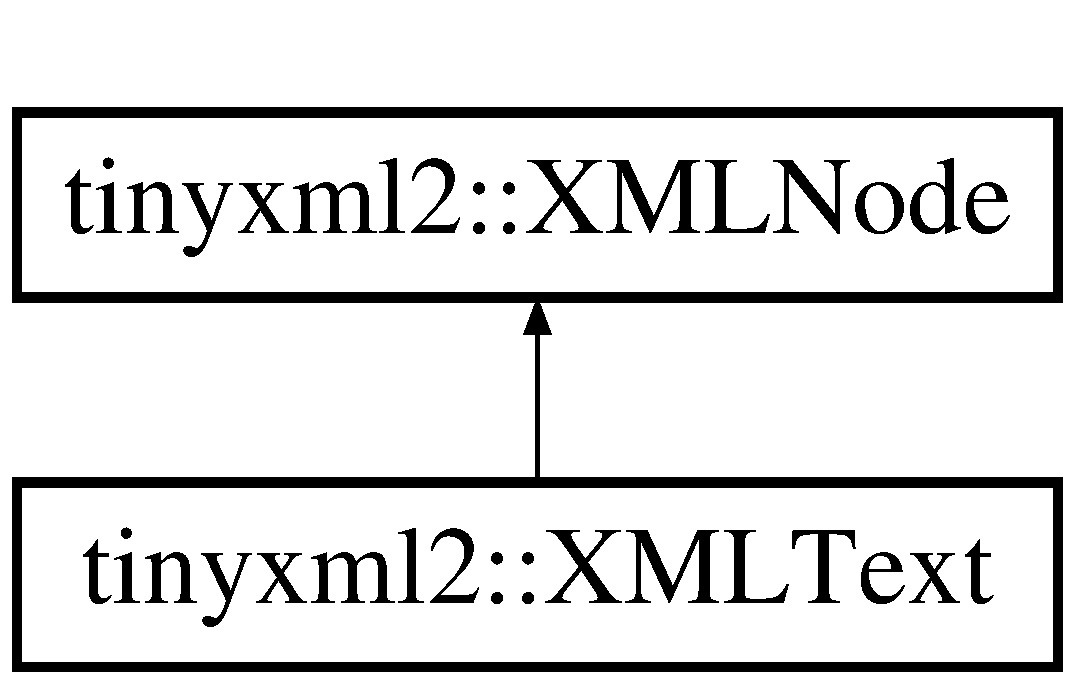
\includegraphics[height=2.000000cm]{classtinyxml2_1_1_x_m_l_text}
\end{center}
\end{figure}
\subsection*{Public Member Functions}
\begin{DoxyCompactItemize}
\item 
virtual bool \mbox{\hyperlink{classtinyxml2_1_1_x_m_l_text_a537c60d7e18fb59c45ac2737a29ac47a}{Accept}} (\mbox{\hyperlink{classtinyxml2_1_1_x_m_l_visitor}{X\+M\+L\+Visitor}} $\ast$visitor) const
\item 
virtual \mbox{\hyperlink{classtinyxml2_1_1_x_m_l_text}{X\+M\+L\+Text}} $\ast$ \mbox{\hyperlink{classtinyxml2_1_1_x_m_l_text_ab1213b4ddebe9b17ec7e7040e9f1caf7}{To\+Text}} ()
\begin{DoxyCompactList}\small\item\em Safely cast to Text, or null. \end{DoxyCompactList}\item 
virtual const \mbox{\hyperlink{classtinyxml2_1_1_x_m_l_text}{X\+M\+L\+Text}} $\ast$ \mbox{\hyperlink{classtinyxml2_1_1_x_m_l_text_a671ce22c7c5ef378f1ce31e6f827b9e2}{To\+Text}} () const
\item 
void \mbox{\hyperlink{classtinyxml2_1_1_x_m_l_text_ad080357d76ab7cc59d7651249949329d}{Set\+C\+Data}} (bool is\+C\+Data)
\begin{DoxyCompactList}\small\item\em Declare whether this should be C\+D\+A\+TA or standard text. \end{DoxyCompactList}\item 
bool \mbox{\hyperlink{classtinyxml2_1_1_x_m_l_text_ac1bb5ea4166c320882d9e0ad16fd385b}{C\+Data}} () const
\begin{DoxyCompactList}\small\item\em Returns true if this is a C\+D\+A\+TA text element. \end{DoxyCompactList}\item 
virtual \mbox{\hyperlink{classtinyxml2_1_1_x_m_l_node}{X\+M\+L\+Node}} $\ast$ \mbox{\hyperlink{classtinyxml2_1_1_x_m_l_text_a86d265c93152726c8c6831e9594840e6}{Shallow\+Clone}} (\mbox{\hyperlink{classtinyxml2_1_1_x_m_l_document}{X\+M\+L\+Document}} $\ast$document) const
\item 
virtual bool \mbox{\hyperlink{classtinyxml2_1_1_x_m_l_text_a99d8bce4dc01df889126e047f358cdfc}{Shallow\+Equal}} (const \mbox{\hyperlink{classtinyxml2_1_1_x_m_l_node}{X\+M\+L\+Node}} $\ast$compare) const
\end{DoxyCompactItemize}
\subsection*{Protected Member Functions}
\begin{DoxyCompactItemize}
\item 
\mbox{\hyperlink{classtinyxml2_1_1_x_m_l_text_ad9f46d70e61e5386ead93728d8b90267}{X\+M\+L\+Text}} (\mbox{\hyperlink{classtinyxml2_1_1_x_m_l_document}{X\+M\+L\+Document}} $\ast$doc)
\item 
virtual \mbox{\hyperlink{classtinyxml2_1_1_x_m_l_text_ae9b8790d0dc13914394dbd7437c0e59d}{$\sim$\+X\+M\+L\+Text}} ()
\item 
char $\ast$ \mbox{\hyperlink{classtinyxml2_1_1_x_m_l_text_af3b93344f1183482e1683f5922ac9c68}{Parse\+Deep}} (char $\ast$p, \mbox{\hyperlink{classtinyxml2_1_1_str_pair}{Str\+Pair}} $\ast$parent\+End\+Tag, int $\ast$cur\+Line\+Num\+Ptr)
\end{DoxyCompactItemize}
\subsection*{Friends}
\begin{DoxyCompactItemize}
\item 
class \mbox{\hyperlink{classtinyxml2_1_1_x_m_l_text_a4eee3bda60c60a30e4e8cd4ea91c4c6e}{X\+M\+L\+Document}}
\end{DoxyCompactItemize}
\subsection*{Additional Inherited Members}


\subsection{Detailed Description}
X\+ML text.

Note that a text node can have child element nodes, for example\+: \begin{DoxyVerb}<root>This is <b>bold</b></root>
\end{DoxyVerb}


A text node can have 2 ways to output the next. \char`\"{}normal\char`\"{} output and C\+D\+A\+TA. It will default to the mode it was parsed from the X\+ML file and you generally want to leave it alone, but you can change the output mode with \mbox{\hyperlink{classtinyxml2_1_1_x_m_l_text_ad080357d76ab7cc59d7651249949329d}{Set\+C\+Data()}} and query it with \mbox{\hyperlink{classtinyxml2_1_1_x_m_l_text_ac1bb5ea4166c320882d9e0ad16fd385b}{C\+Data()}}. 

\subsection{Constructor \& Destructor Documentation}
\mbox{\Hypertarget{classtinyxml2_1_1_x_m_l_text_ad9f46d70e61e5386ead93728d8b90267}\label{classtinyxml2_1_1_x_m_l_text_ad9f46d70e61e5386ead93728d8b90267}} 
\index{tinyxml2\+::\+X\+M\+L\+Text@{tinyxml2\+::\+X\+M\+L\+Text}!X\+M\+L\+Text@{X\+M\+L\+Text}}
\index{X\+M\+L\+Text@{X\+M\+L\+Text}!tinyxml2\+::\+X\+M\+L\+Text@{tinyxml2\+::\+X\+M\+L\+Text}}
\subsubsection{\texorpdfstring{X\+M\+L\+Text()}{XMLText()}}
{\footnotesize\ttfamily tinyxml2\+::\+X\+M\+L\+Text\+::\+X\+M\+L\+Text (\begin{DoxyParamCaption}\item[{\mbox{\hyperlink{classtinyxml2_1_1_x_m_l_document}{X\+M\+L\+Document}} $\ast$}]{doc }\end{DoxyParamCaption})\hspace{0.3cm}{\ttfamily [inline]}, {\ttfamily [protected]}}

\mbox{\Hypertarget{classtinyxml2_1_1_x_m_l_text_ae9b8790d0dc13914394dbd7437c0e59d}\label{classtinyxml2_1_1_x_m_l_text_ae9b8790d0dc13914394dbd7437c0e59d}} 
\index{tinyxml2\+::\+X\+M\+L\+Text@{tinyxml2\+::\+X\+M\+L\+Text}!````~X\+M\+L\+Text@{$\sim$\+X\+M\+L\+Text}}
\index{````~X\+M\+L\+Text@{$\sim$\+X\+M\+L\+Text}!tinyxml2\+::\+X\+M\+L\+Text@{tinyxml2\+::\+X\+M\+L\+Text}}
\subsubsection{\texorpdfstring{$\sim$\+X\+M\+L\+Text()}{~XMLText()}}
{\footnotesize\ttfamily virtual tinyxml2\+::\+X\+M\+L\+Text\+::$\sim$\+X\+M\+L\+Text (\begin{DoxyParamCaption}{ }\end{DoxyParamCaption})\hspace{0.3cm}{\ttfamily [inline]}, {\ttfamily [protected]}, {\ttfamily [virtual]}}



\subsection{Member Function Documentation}
\mbox{\Hypertarget{classtinyxml2_1_1_x_m_l_text_a537c60d7e18fb59c45ac2737a29ac47a}\label{classtinyxml2_1_1_x_m_l_text_a537c60d7e18fb59c45ac2737a29ac47a}} 
\index{tinyxml2\+::\+X\+M\+L\+Text@{tinyxml2\+::\+X\+M\+L\+Text}!Accept@{Accept}}
\index{Accept@{Accept}!tinyxml2\+::\+X\+M\+L\+Text@{tinyxml2\+::\+X\+M\+L\+Text}}
\subsubsection{\texorpdfstring{Accept()}{Accept()}}
{\footnotesize\ttfamily bool tinyxml2\+::\+X\+M\+L\+Text\+::\+Accept (\begin{DoxyParamCaption}\item[{\mbox{\hyperlink{classtinyxml2_1_1_x_m_l_visitor}{X\+M\+L\+Visitor}} $\ast$}]{visitor }\end{DoxyParamCaption}) const\hspace{0.3cm}{\ttfamily [virtual]}}

Accept a hierarchical visit of the nodes in the Tiny\+X\+M\+L-\/2 D\+OM. Every node in the X\+ML tree will be conditionally visited and the host will be called back via the \mbox{\hyperlink{classtinyxml2_1_1_x_m_l_visitor}{X\+M\+L\+Visitor}} interface.

This is essentially a S\+AX interface for Tiny\+X\+M\+L-\/2. (Note however it doesn\textquotesingle{}t re-\/parse the X\+ML for the callbacks, so the performance of Tiny\+X\+M\+L-\/2 is unchanged by using this interface versus any other.)

The interface has been based on ideas from\+:


\begin{DoxyItemize}
\item \href{http://www.saxproject.org/}{\tt http\+://www.\+saxproject.\+org/}
\item \href{http://c2.com/cgi/wiki?HierarchicalVisitorPattern}{\tt http\+://c2.\+com/cgi/wiki?\+Hierarchical\+Visitor\+Pattern}
\end{DoxyItemize}

Which are both good references for \char`\"{}visiting\char`\"{}.

An example of using \mbox{\hyperlink{classtinyxml2_1_1_x_m_l_text_a537c60d7e18fb59c45ac2737a29ac47a}{Accept()}}\+: \begin{DoxyVerb}XMLPrinter printer;
tinyxmlDoc.Accept( &printer );
const char* xmlcstr = printer.CStr();
\end{DoxyVerb}
 

Implements \mbox{\hyperlink{classtinyxml2_1_1_x_m_l_node_a81e66df0a44c67a7af17f3b77a152785}{tinyxml2\+::\+X\+M\+L\+Node}}.

\mbox{\Hypertarget{classtinyxml2_1_1_x_m_l_text_ac1bb5ea4166c320882d9e0ad16fd385b}\label{classtinyxml2_1_1_x_m_l_text_ac1bb5ea4166c320882d9e0ad16fd385b}} 
\index{tinyxml2\+::\+X\+M\+L\+Text@{tinyxml2\+::\+X\+M\+L\+Text}!C\+Data@{C\+Data}}
\index{C\+Data@{C\+Data}!tinyxml2\+::\+X\+M\+L\+Text@{tinyxml2\+::\+X\+M\+L\+Text}}
\subsubsection{\texorpdfstring{C\+Data()}{CData()}}
{\footnotesize\ttfamily bool tinyxml2\+::\+X\+M\+L\+Text\+::\+C\+Data (\begin{DoxyParamCaption}{ }\end{DoxyParamCaption}) const\hspace{0.3cm}{\ttfamily [inline]}}



Returns true if this is a C\+D\+A\+TA text element. 

\mbox{\Hypertarget{classtinyxml2_1_1_x_m_l_text_af3b93344f1183482e1683f5922ac9c68}\label{classtinyxml2_1_1_x_m_l_text_af3b93344f1183482e1683f5922ac9c68}} 
\index{tinyxml2\+::\+X\+M\+L\+Text@{tinyxml2\+::\+X\+M\+L\+Text}!Parse\+Deep@{Parse\+Deep}}
\index{Parse\+Deep@{Parse\+Deep}!tinyxml2\+::\+X\+M\+L\+Text@{tinyxml2\+::\+X\+M\+L\+Text}}
\subsubsection{\texorpdfstring{Parse\+Deep()}{ParseDeep()}}
{\footnotesize\ttfamily char $\ast$ tinyxml2\+::\+X\+M\+L\+Text\+::\+Parse\+Deep (\begin{DoxyParamCaption}\item[{char $\ast$}]{p,  }\item[{\mbox{\hyperlink{classtinyxml2_1_1_str_pair}{Str\+Pair}} $\ast$}]{parent\+End\+Tag,  }\item[{int $\ast$}]{cur\+Line\+Num\+Ptr }\end{DoxyParamCaption})\hspace{0.3cm}{\ttfamily [protected]}, {\ttfamily [virtual]}}



Reimplemented from \mbox{\hyperlink{classtinyxml2_1_1_x_m_l_node_a916e498914baecbc9a1f012352ef7c69}{tinyxml2\+::\+X\+M\+L\+Node}}.

\mbox{\Hypertarget{classtinyxml2_1_1_x_m_l_text_ad080357d76ab7cc59d7651249949329d}\label{classtinyxml2_1_1_x_m_l_text_ad080357d76ab7cc59d7651249949329d}} 
\index{tinyxml2\+::\+X\+M\+L\+Text@{tinyxml2\+::\+X\+M\+L\+Text}!Set\+C\+Data@{Set\+C\+Data}}
\index{Set\+C\+Data@{Set\+C\+Data}!tinyxml2\+::\+X\+M\+L\+Text@{tinyxml2\+::\+X\+M\+L\+Text}}
\subsubsection{\texorpdfstring{Set\+C\+Data()}{SetCData()}}
{\footnotesize\ttfamily void tinyxml2\+::\+X\+M\+L\+Text\+::\+Set\+C\+Data (\begin{DoxyParamCaption}\item[{bool}]{is\+C\+Data }\end{DoxyParamCaption})\hspace{0.3cm}{\ttfamily [inline]}}



Declare whether this should be C\+D\+A\+TA or standard text. 

\mbox{\Hypertarget{classtinyxml2_1_1_x_m_l_text_a86d265c93152726c8c6831e9594840e6}\label{classtinyxml2_1_1_x_m_l_text_a86d265c93152726c8c6831e9594840e6}} 
\index{tinyxml2\+::\+X\+M\+L\+Text@{tinyxml2\+::\+X\+M\+L\+Text}!Shallow\+Clone@{Shallow\+Clone}}
\index{Shallow\+Clone@{Shallow\+Clone}!tinyxml2\+::\+X\+M\+L\+Text@{tinyxml2\+::\+X\+M\+L\+Text}}
\subsubsection{\texorpdfstring{Shallow\+Clone()}{ShallowClone()}}
{\footnotesize\ttfamily \mbox{\hyperlink{classtinyxml2_1_1_x_m_l_node}{X\+M\+L\+Node}} $\ast$ tinyxml2\+::\+X\+M\+L\+Text\+::\+Shallow\+Clone (\begin{DoxyParamCaption}\item[{\mbox{\hyperlink{classtinyxml2_1_1_x_m_l_document}{X\+M\+L\+Document}} $\ast$}]{document }\end{DoxyParamCaption}) const\hspace{0.3cm}{\ttfamily [virtual]}}

Make a copy of this node, but not its children. You may pass in a Document pointer that will be the owner of the new Node. If the \textquotesingle{}document\textquotesingle{} is null, then the node returned will be allocated from the current Document. (this-\/$>$\mbox{\hyperlink{classtinyxml2_1_1_x_m_l_node_af343d1ef0b45c0020e62d784d7e67a68}{Get\+Document()}})

Note\+: if called on a \mbox{\hyperlink{classtinyxml2_1_1_x_m_l_document}{X\+M\+L\+Document}}, this will return null. 

Implements \mbox{\hyperlink{classtinyxml2_1_1_x_m_l_node_a8402cbd3129d20e9e6024bbcc0531283}{tinyxml2\+::\+X\+M\+L\+Node}}.

\mbox{\Hypertarget{classtinyxml2_1_1_x_m_l_text_a99d8bce4dc01df889126e047f358cdfc}\label{classtinyxml2_1_1_x_m_l_text_a99d8bce4dc01df889126e047f358cdfc}} 
\index{tinyxml2\+::\+X\+M\+L\+Text@{tinyxml2\+::\+X\+M\+L\+Text}!Shallow\+Equal@{Shallow\+Equal}}
\index{Shallow\+Equal@{Shallow\+Equal}!tinyxml2\+::\+X\+M\+L\+Text@{tinyxml2\+::\+X\+M\+L\+Text}}
\subsubsection{\texorpdfstring{Shallow\+Equal()}{ShallowEqual()}}
{\footnotesize\ttfamily bool tinyxml2\+::\+X\+M\+L\+Text\+::\+Shallow\+Equal (\begin{DoxyParamCaption}\item[{const \mbox{\hyperlink{classtinyxml2_1_1_x_m_l_node}{X\+M\+L\+Node}} $\ast$}]{compare }\end{DoxyParamCaption}) const\hspace{0.3cm}{\ttfamily [virtual]}}

Test if 2 nodes are the same, but don\textquotesingle{}t test children. The 2 nodes do not need to be in the same Document.

Note\+: if called on a \mbox{\hyperlink{classtinyxml2_1_1_x_m_l_document}{X\+M\+L\+Document}}, this will return false. 

Implements \mbox{\hyperlink{classtinyxml2_1_1_x_m_l_node_a7ce18b751c3ea09eac292dca264f9226}{tinyxml2\+::\+X\+M\+L\+Node}}.

\mbox{\Hypertarget{classtinyxml2_1_1_x_m_l_text_ab1213b4ddebe9b17ec7e7040e9f1caf7}\label{classtinyxml2_1_1_x_m_l_text_ab1213b4ddebe9b17ec7e7040e9f1caf7}} 
\index{tinyxml2\+::\+X\+M\+L\+Text@{tinyxml2\+::\+X\+M\+L\+Text}!To\+Text@{To\+Text}}
\index{To\+Text@{To\+Text}!tinyxml2\+::\+X\+M\+L\+Text@{tinyxml2\+::\+X\+M\+L\+Text}}
\subsubsection{\texorpdfstring{To\+Text()}{ToText()}\hspace{0.1cm}{\footnotesize\ttfamily [1/2]}}
{\footnotesize\ttfamily virtual \mbox{\hyperlink{classtinyxml2_1_1_x_m_l_text}{X\+M\+L\+Text}}$\ast$ tinyxml2\+::\+X\+M\+L\+Text\+::\+To\+Text (\begin{DoxyParamCaption}{ }\end{DoxyParamCaption})\hspace{0.3cm}{\ttfamily [inline]}, {\ttfamily [virtual]}}



Safely cast to Text, or null. 



Reimplemented from \mbox{\hyperlink{classtinyxml2_1_1_x_m_l_node_a41c55dab9162d1eb62db2008430e376b}{tinyxml2\+::\+X\+M\+L\+Node}}.

\mbox{\Hypertarget{classtinyxml2_1_1_x_m_l_text_a671ce22c7c5ef378f1ce31e6f827b9e2}\label{classtinyxml2_1_1_x_m_l_text_a671ce22c7c5ef378f1ce31e6f827b9e2}} 
\index{tinyxml2\+::\+X\+M\+L\+Text@{tinyxml2\+::\+X\+M\+L\+Text}!To\+Text@{To\+Text}}
\index{To\+Text@{To\+Text}!tinyxml2\+::\+X\+M\+L\+Text@{tinyxml2\+::\+X\+M\+L\+Text}}
\subsubsection{\texorpdfstring{To\+Text()}{ToText()}\hspace{0.1cm}{\footnotesize\ttfamily [2/2]}}
{\footnotesize\ttfamily virtual const \mbox{\hyperlink{classtinyxml2_1_1_x_m_l_text}{X\+M\+L\+Text}}$\ast$ tinyxml2\+::\+X\+M\+L\+Text\+::\+To\+Text (\begin{DoxyParamCaption}{ }\end{DoxyParamCaption}) const\hspace{0.3cm}{\ttfamily [inline]}, {\ttfamily [virtual]}}



Reimplemented from \mbox{\hyperlink{classtinyxml2_1_1_x_m_l_node_acb9ccc1beda27c0efcb0545683c3e7f4}{tinyxml2\+::\+X\+M\+L\+Node}}.



\subsection{Friends And Related Function Documentation}
\mbox{\Hypertarget{classtinyxml2_1_1_x_m_l_text_a4eee3bda60c60a30e4e8cd4ea91c4c6e}\label{classtinyxml2_1_1_x_m_l_text_a4eee3bda60c60a30e4e8cd4ea91c4c6e}} 
\index{tinyxml2\+::\+X\+M\+L\+Text@{tinyxml2\+::\+X\+M\+L\+Text}!X\+M\+L\+Document@{X\+M\+L\+Document}}
\index{X\+M\+L\+Document@{X\+M\+L\+Document}!tinyxml2\+::\+X\+M\+L\+Text@{tinyxml2\+::\+X\+M\+L\+Text}}
\subsubsection{\texorpdfstring{X\+M\+L\+Document}{XMLDocument}}
{\footnotesize\ttfamily friend class \mbox{\hyperlink{classtinyxml2_1_1_x_m_l_document}{X\+M\+L\+Document}}\hspace{0.3cm}{\ttfamily [friend]}}



The documentation for this class was generated from the following files\+:\begin{DoxyCompactItemize}
\item 
\mbox{\hyperlink{tinyxml2_8h}{tinyxml2.\+h}}\item 
\mbox{\hyperlink{tinyxml2_8cpp}{tinyxml2.\+cpp}}\end{DoxyCompactItemize}

\hypertarget{classtinyxml2_1_1_x_m_l_unknown}{}\section{tinyxml2\+:\+:X\+M\+L\+Unknown Class Reference}
\label{classtinyxml2_1_1_x_m_l_unknown}\index{tinyxml2\+::\+X\+M\+L\+Unknown@{tinyxml2\+::\+X\+M\+L\+Unknown}}


{\ttfamily \#include $<$tinyxml2.\+h$>$}

Inheritance diagram for tinyxml2\+:\+:X\+M\+L\+Unknown\+:\begin{figure}[H]
\begin{center}
\leavevmode
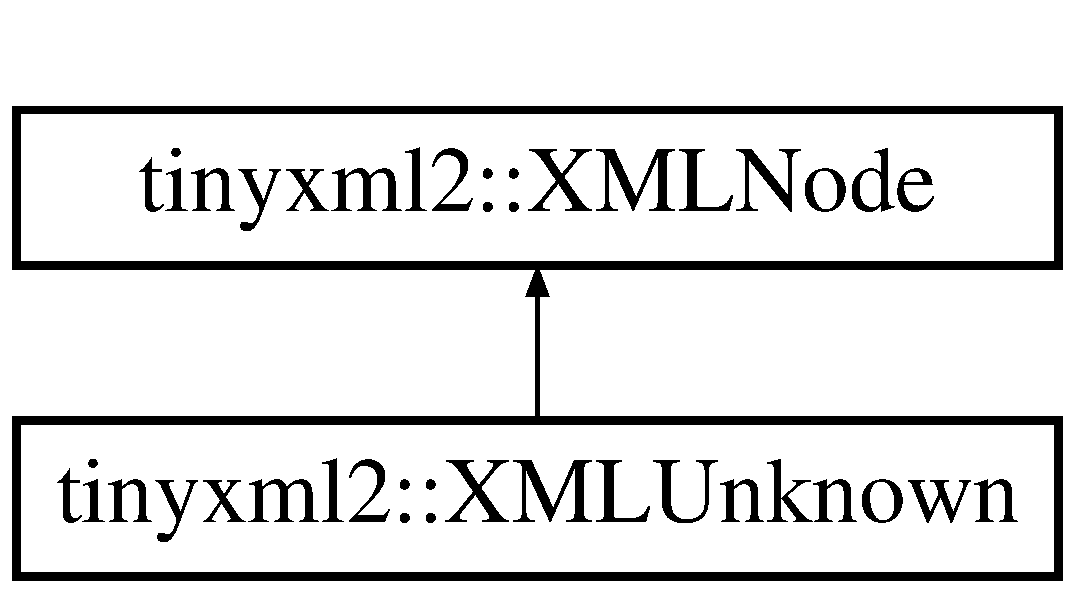
\includegraphics[height=2.000000cm]{classtinyxml2_1_1_x_m_l_unknown}
\end{center}
\end{figure}
\subsection*{Public Member Functions}
\begin{DoxyCompactItemize}
\item 
\mbox{\Hypertarget{classtinyxml2_1_1_x_m_l_unknown_af4374856421921cad578c8affae872b6}\label{classtinyxml2_1_1_x_m_l_unknown_af4374856421921cad578c8affae872b6}} 
virtual \mbox{\hyperlink{classtinyxml2_1_1_x_m_l_unknown}{X\+M\+L\+Unknown}} $\ast$ \mbox{\hyperlink{classtinyxml2_1_1_x_m_l_unknown_af4374856421921cad578c8affae872b6}{To\+Unknown}} ()
\begin{DoxyCompactList}\small\item\em Safely cast to an Unknown, or null. \end{DoxyCompactList}\item 
\mbox{\Hypertarget{classtinyxml2_1_1_x_m_l_unknown_a61b342b4f295cded1dc2f4402e97f07e}\label{classtinyxml2_1_1_x_m_l_unknown_a61b342b4f295cded1dc2f4402e97f07e}} 
virtual const \mbox{\hyperlink{classtinyxml2_1_1_x_m_l_unknown}{X\+M\+L\+Unknown}} $\ast$ {\bfseries To\+Unknown} () const
\item 
virtual bool \mbox{\hyperlink{classtinyxml2_1_1_x_m_l_unknown_a8a06b8c82117ca969a432e17a46830fc}{Accept}} (\mbox{\hyperlink{classtinyxml2_1_1_x_m_l_visitor}{X\+M\+L\+Visitor}} $\ast$visitor) const
\item 
virtual \mbox{\hyperlink{classtinyxml2_1_1_x_m_l_node}{X\+M\+L\+Node}} $\ast$ \mbox{\hyperlink{classtinyxml2_1_1_x_m_l_unknown_ab73b48b819aa4b2ef3815dc2d7d20d5f}{Shallow\+Clone}} (\mbox{\hyperlink{classtinyxml2_1_1_x_m_l_document}{X\+M\+L\+Document}} $\ast$document) const
\item 
virtual bool \mbox{\hyperlink{classtinyxml2_1_1_x_m_l_unknown_ac46767cd721d666e690a6231dfb618d1}{Shallow\+Equal}} (const \mbox{\hyperlink{classtinyxml2_1_1_x_m_l_node}{X\+M\+L\+Node}} $\ast$compare) const
\end{DoxyCompactItemize}
\subsection*{Protected Member Functions}
\begin{DoxyCompactItemize}
\item 
\mbox{\Hypertarget{classtinyxml2_1_1_x_m_l_unknown_a9391eb679598d50baba424e6f1aa367b}\label{classtinyxml2_1_1_x_m_l_unknown_a9391eb679598d50baba424e6f1aa367b}} 
{\bfseries X\+M\+L\+Unknown} (\mbox{\hyperlink{classtinyxml2_1_1_x_m_l_document}{X\+M\+L\+Document}} $\ast$doc)
\item 
\mbox{\Hypertarget{classtinyxml2_1_1_x_m_l_unknown_aefc332cc1e6e25736f364d1e5eeb31fe}\label{classtinyxml2_1_1_x_m_l_unknown_aefc332cc1e6e25736f364d1e5eeb31fe}} 
char $\ast$ {\bfseries Parse\+Deep} (char $\ast$p, \mbox{\hyperlink{classtinyxml2_1_1_str_pair}{Str\+Pair}} $\ast$parent\+End\+Tag, int $\ast$cur\+Line\+Num\+Ptr)
\end{DoxyCompactItemize}
\subsection*{Friends}
\begin{DoxyCompactItemize}
\item 
\mbox{\Hypertarget{classtinyxml2_1_1_x_m_l_unknown_a4eee3bda60c60a30e4e8cd4ea91c4c6e}\label{classtinyxml2_1_1_x_m_l_unknown_a4eee3bda60c60a30e4e8cd4ea91c4c6e}} 
class {\bfseries X\+M\+L\+Document}
\end{DoxyCompactItemize}
\subsection*{Additional Inherited Members}


\subsection{Detailed Description}
Any tag that Tiny\+X\+M\+L-\/2 doesn\textquotesingle{}t recognize is saved as an unknown. It is a tag of text, but should not be modified. It will be written back to the X\+ML, unchanged, when the file is saved.

D\+TD tags get thrown into X\+M\+L\+Unknowns. 

\subsection{Member Function Documentation}
\mbox{\Hypertarget{classtinyxml2_1_1_x_m_l_unknown_a8a06b8c82117ca969a432e17a46830fc}\label{classtinyxml2_1_1_x_m_l_unknown_a8a06b8c82117ca969a432e17a46830fc}} 
\index{tinyxml2\+::\+X\+M\+L\+Unknown@{tinyxml2\+::\+X\+M\+L\+Unknown}!Accept@{Accept}}
\index{Accept@{Accept}!tinyxml2\+::\+X\+M\+L\+Unknown@{tinyxml2\+::\+X\+M\+L\+Unknown}}
\subsubsection{\texorpdfstring{Accept()}{Accept()}}
{\footnotesize\ttfamily bool tinyxml2\+::\+X\+M\+L\+Unknown\+::\+Accept (\begin{DoxyParamCaption}\item[{\mbox{\hyperlink{classtinyxml2_1_1_x_m_l_visitor}{X\+M\+L\+Visitor}} $\ast$}]{visitor }\end{DoxyParamCaption}) const\hspace{0.3cm}{\ttfamily [virtual]}}

Accept a hierarchical visit of the nodes in the Tiny\+X\+M\+L-\/2 D\+OM. Every node in the X\+ML tree will be conditionally visited and the host will be called back via the \mbox{\hyperlink{classtinyxml2_1_1_x_m_l_visitor}{X\+M\+L\+Visitor}} interface.

This is essentially a S\+AX interface for Tiny\+X\+M\+L-\/2. (Note however it doesn\textquotesingle{}t re-\/parse the X\+ML for the callbacks, so the performance of Tiny\+X\+M\+L-\/2 is unchanged by using this interface versus any other.)

The interface has been based on ideas from\+:


\begin{DoxyItemize}
\item \href{http://www.saxproject.org/}{\tt http\+://www.\+saxproject.\+org/}
\item \href{http://c2.com/cgi/wiki?HierarchicalVisitorPattern}{\tt http\+://c2.\+com/cgi/wiki?\+Hierarchical\+Visitor\+Pattern}
\end{DoxyItemize}

Which are both good references for \char`\"{}visiting\char`\"{}.

An example of using \mbox{\hyperlink{classtinyxml2_1_1_x_m_l_unknown_a8a06b8c82117ca969a432e17a46830fc}{Accept()}}\+: \begin{DoxyVerb}XMLPrinter printer;
tinyxmlDoc.Accept( &printer );
const char* xmlcstr = printer.CStr();
\end{DoxyVerb}
 

Implements \mbox{\hyperlink{classtinyxml2_1_1_x_m_l_node_a81e66df0a44c67a7af17f3b77a152785}{tinyxml2\+::\+X\+M\+L\+Node}}.

\mbox{\Hypertarget{classtinyxml2_1_1_x_m_l_unknown_ab73b48b819aa4b2ef3815dc2d7d20d5f}\label{classtinyxml2_1_1_x_m_l_unknown_ab73b48b819aa4b2ef3815dc2d7d20d5f}} 
\index{tinyxml2\+::\+X\+M\+L\+Unknown@{tinyxml2\+::\+X\+M\+L\+Unknown}!Shallow\+Clone@{Shallow\+Clone}}
\index{Shallow\+Clone@{Shallow\+Clone}!tinyxml2\+::\+X\+M\+L\+Unknown@{tinyxml2\+::\+X\+M\+L\+Unknown}}
\subsubsection{\texorpdfstring{Shallow\+Clone()}{ShallowClone()}}
{\footnotesize\ttfamily \mbox{\hyperlink{classtinyxml2_1_1_x_m_l_node}{X\+M\+L\+Node}} $\ast$ tinyxml2\+::\+X\+M\+L\+Unknown\+::\+Shallow\+Clone (\begin{DoxyParamCaption}\item[{\mbox{\hyperlink{classtinyxml2_1_1_x_m_l_document}{X\+M\+L\+Document}} $\ast$}]{document }\end{DoxyParamCaption}) const\hspace{0.3cm}{\ttfamily [virtual]}}

Make a copy of this node, but not its children. You may pass in a Document pointer that will be the owner of the new Node. If the \textquotesingle{}document\textquotesingle{} is null, then the node returned will be allocated from the current Document. (this-\/$>$\mbox{\hyperlink{classtinyxml2_1_1_x_m_l_node_af343d1ef0b45c0020e62d784d7e67a68}{Get\+Document()}})

Note\+: if called on a \mbox{\hyperlink{classtinyxml2_1_1_x_m_l_document}{X\+M\+L\+Document}}, this will return null. 

Implements \mbox{\hyperlink{classtinyxml2_1_1_x_m_l_node_a8402cbd3129d20e9e6024bbcc0531283}{tinyxml2\+::\+X\+M\+L\+Node}}.

\mbox{\Hypertarget{classtinyxml2_1_1_x_m_l_unknown_ac46767cd721d666e690a6231dfb618d1}\label{classtinyxml2_1_1_x_m_l_unknown_ac46767cd721d666e690a6231dfb618d1}} 
\index{tinyxml2\+::\+X\+M\+L\+Unknown@{tinyxml2\+::\+X\+M\+L\+Unknown}!Shallow\+Equal@{Shallow\+Equal}}
\index{Shallow\+Equal@{Shallow\+Equal}!tinyxml2\+::\+X\+M\+L\+Unknown@{tinyxml2\+::\+X\+M\+L\+Unknown}}
\subsubsection{\texorpdfstring{Shallow\+Equal()}{ShallowEqual()}}
{\footnotesize\ttfamily bool tinyxml2\+::\+X\+M\+L\+Unknown\+::\+Shallow\+Equal (\begin{DoxyParamCaption}\item[{const \mbox{\hyperlink{classtinyxml2_1_1_x_m_l_node}{X\+M\+L\+Node}} $\ast$}]{compare }\end{DoxyParamCaption}) const\hspace{0.3cm}{\ttfamily [virtual]}}

Test if 2 nodes are the same, but don\textquotesingle{}t test children. The 2 nodes do not need to be in the same Document.

Note\+: if called on a \mbox{\hyperlink{classtinyxml2_1_1_x_m_l_document}{X\+M\+L\+Document}}, this will return false. 

Implements \mbox{\hyperlink{classtinyxml2_1_1_x_m_l_node_a7ce18b751c3ea09eac292dca264f9226}{tinyxml2\+::\+X\+M\+L\+Node}}.



The documentation for this class was generated from the following files\+:\begin{DoxyCompactItemize}
\item 
tinyxml2.\+h\item 
tinyxml2.\+cpp\end{DoxyCompactItemize}

\hypertarget{classtinyxml2_1_1_x_m_l_util}{}\section{tinyxml2\+:\+:X\+M\+L\+Util Class Reference}
\label{classtinyxml2_1_1_x_m_l_util}\index{tinyxml2\+::\+X\+M\+L\+Util@{tinyxml2\+::\+X\+M\+L\+Util}}
\subsection*{Static Public Member Functions}
\begin{DoxyCompactItemize}
\item 
\mbox{\Hypertarget{classtinyxml2_1_1_x_m_l_util_ab626a194b3523a5ba8b9dbaa2a165202}\label{classtinyxml2_1_1_x_m_l_util_ab626a194b3523a5ba8b9dbaa2a165202}} 
static const char $\ast$ {\bfseries Skip\+White\+Space} (const char $\ast$p, int $\ast$cur\+Line\+Num\+Ptr)
\item 
\mbox{\Hypertarget{classtinyxml2_1_1_x_m_l_util_abb6cb3e71f88efca82cb7157367fd91e}\label{classtinyxml2_1_1_x_m_l_util_abb6cb3e71f88efca82cb7157367fd91e}} 
static char $\ast$ {\bfseries Skip\+White\+Space} (char $\ast$p, int $\ast$cur\+Line\+Num\+Ptr)
\item 
\mbox{\Hypertarget{classtinyxml2_1_1_x_m_l_util_a357ec3af8fc433d19023a815f45e8e33}\label{classtinyxml2_1_1_x_m_l_util_a357ec3af8fc433d19023a815f45e8e33}} 
static bool {\bfseries Is\+White\+Space} (char p)
\item 
\mbox{\Hypertarget{classtinyxml2_1_1_x_m_l_util_abe106a69ac4d942a4381a4d9dfd0e0bd}\label{classtinyxml2_1_1_x_m_l_util_abe106a69ac4d942a4381a4d9dfd0e0bd}} 
static bool {\bfseries Is\+Name\+Start\+Char} (unsigned char ch)
\item 
\mbox{\Hypertarget{classtinyxml2_1_1_x_m_l_util_a04b17341538fa11752f24b4301d19485}\label{classtinyxml2_1_1_x_m_l_util_a04b17341538fa11752f24b4301d19485}} 
static bool {\bfseries Is\+Name\+Char} (unsigned char ch)
\item 
\mbox{\Hypertarget{classtinyxml2_1_1_x_m_l_util_acfcd287cacfd2533e1bc9ea4dfb56602}\label{classtinyxml2_1_1_x_m_l_util_acfcd287cacfd2533e1bc9ea4dfb56602}} 
static bool {\bfseries String\+Equal} (const char $\ast$p, const char $\ast$q, int n\+Char=I\+N\+T\+\_\+\+M\+AX)
\item 
\mbox{\Hypertarget{classtinyxml2_1_1_x_m_l_util_ad7fd82e0fe610d73ef7bf9f359f104a3}\label{classtinyxml2_1_1_x_m_l_util_ad7fd82e0fe610d73ef7bf9f359f104a3}} 
static bool {\bfseries Is\+U\+T\+F8\+Continuation} (char p)
\item 
\mbox{\Hypertarget{classtinyxml2_1_1_x_m_l_util_ae9bcb2bc3cd6475fdc644c8c17790555}\label{classtinyxml2_1_1_x_m_l_util_ae9bcb2bc3cd6475fdc644c8c17790555}} 
static const char $\ast$ {\bfseries Read\+B\+OM} (const char $\ast$p, bool $\ast$has\+B\+OM)
\item 
\mbox{\Hypertarget{classtinyxml2_1_1_x_m_l_util_a5a96e5144a8d693dc4bcd783d9964648}\label{classtinyxml2_1_1_x_m_l_util_a5a96e5144a8d693dc4bcd783d9964648}} 
static const char $\ast$ {\bfseries Get\+Character\+Ref} (const char $\ast$p, char $\ast$value, int $\ast$length)
\item 
\mbox{\Hypertarget{classtinyxml2_1_1_x_m_l_util_a31c00d5c5dfb38382de1dfcaf4be3595}\label{classtinyxml2_1_1_x_m_l_util_a31c00d5c5dfb38382de1dfcaf4be3595}} 
static void {\bfseries Convert\+U\+T\+F32\+To\+U\+T\+F8} (unsigned long input, char $\ast$output, int $\ast$length)
\item 
\mbox{\Hypertarget{classtinyxml2_1_1_x_m_l_util_a3cd6c703d49b9d51bdf0f4ff6aa021c7}\label{classtinyxml2_1_1_x_m_l_util_a3cd6c703d49b9d51bdf0f4ff6aa021c7}} 
static void {\bfseries To\+Str} (int v, char $\ast$buffer, int buffer\+Size)
\item 
\mbox{\Hypertarget{classtinyxml2_1_1_x_m_l_util_ac00c2e52c1c36dab3ff41d86a9bf60f9}\label{classtinyxml2_1_1_x_m_l_util_ac00c2e52c1c36dab3ff41d86a9bf60f9}} 
static void {\bfseries To\+Str} (unsigned v, char $\ast$buffer, int buffer\+Size)
\item 
\mbox{\Hypertarget{classtinyxml2_1_1_x_m_l_util_adba0718527ae9e80f663a71ea325cb11}\label{classtinyxml2_1_1_x_m_l_util_adba0718527ae9e80f663a71ea325cb11}} 
static void {\bfseries To\+Str} (bool v, char $\ast$buffer, int buffer\+Size)
\item 
\mbox{\Hypertarget{classtinyxml2_1_1_x_m_l_util_a8957ad44fee5fa02ba52d73aad4d0a31}\label{classtinyxml2_1_1_x_m_l_util_a8957ad44fee5fa02ba52d73aad4d0a31}} 
static void {\bfseries To\+Str} (float v, char $\ast$buffer, int buffer\+Size)
\item 
\mbox{\Hypertarget{classtinyxml2_1_1_x_m_l_util_a1cd141e50980fcddd6bf9af5de4b1db7}\label{classtinyxml2_1_1_x_m_l_util_a1cd141e50980fcddd6bf9af5de4b1db7}} 
static void {\bfseries To\+Str} (double v, char $\ast$buffer, int buffer\+Size)
\item 
\mbox{\Hypertarget{classtinyxml2_1_1_x_m_l_util_a26a8cb5b833ad587b3af39469c8111de}\label{classtinyxml2_1_1_x_m_l_util_a26a8cb5b833ad587b3af39469c8111de}} 
static void {\bfseries To\+Str} (int64\+\_\+t v, char $\ast$buffer, int buffer\+Size)
\item 
\mbox{\Hypertarget{classtinyxml2_1_1_x_m_l_util_ad4df4023d11ee3fca9689c49b9707323}\label{classtinyxml2_1_1_x_m_l_util_ad4df4023d11ee3fca9689c49b9707323}} 
static bool {\bfseries To\+Int} (const char $\ast$str, int $\ast$value)
\item 
\mbox{\Hypertarget{classtinyxml2_1_1_x_m_l_util_a210c8637d5eb4ce3d4625294af0efc2f}\label{classtinyxml2_1_1_x_m_l_util_a210c8637d5eb4ce3d4625294af0efc2f}} 
static bool {\bfseries To\+Unsigned} (const char $\ast$str, unsigned $\ast$value)
\item 
\mbox{\Hypertarget{classtinyxml2_1_1_x_m_l_util_ae5b03e0a1ca5d42052a7ac540f7aa12a}\label{classtinyxml2_1_1_x_m_l_util_ae5b03e0a1ca5d42052a7ac540f7aa12a}} 
static bool {\bfseries To\+Bool} (const char $\ast$str, bool $\ast$value)
\item 
\mbox{\Hypertarget{classtinyxml2_1_1_x_m_l_util_a399e71edb5f29d61ea81d91ee0332bb9}\label{classtinyxml2_1_1_x_m_l_util_a399e71edb5f29d61ea81d91ee0332bb9}} 
static bool {\bfseries To\+Float} (const char $\ast$str, float $\ast$value)
\item 
\mbox{\Hypertarget{classtinyxml2_1_1_x_m_l_util_ad8f75ac140fb19c1c6e164a957c4cd53}\label{classtinyxml2_1_1_x_m_l_util_ad8f75ac140fb19c1c6e164a957c4cd53}} 
static bool {\bfseries To\+Double} (const char $\ast$str, double $\ast$value)
\item 
\mbox{\Hypertarget{classtinyxml2_1_1_x_m_l_util_afe2ea09257431cd2b4b6d440552e4195}\label{classtinyxml2_1_1_x_m_l_util_afe2ea09257431cd2b4b6d440552e4195}} 
static bool {\bfseries To\+Int64} (const char $\ast$str, int64\+\_\+t $\ast$value)
\item 
\mbox{\Hypertarget{classtinyxml2_1_1_x_m_l_util_af98a6a80dbeec4679366c1aba4c5b747}\label{classtinyxml2_1_1_x_m_l_util_af98a6a80dbeec4679366c1aba4c5b747}} 
static void {\bfseries Set\+Bool\+Serialization} (const char $\ast$write\+True, const char $\ast$write\+False)
\end{DoxyCompactItemize}


The documentation for this class was generated from the following files\+:\begin{DoxyCompactItemize}
\item 
tinyxml2.\+h\item 
tinyxml2.\+cpp\end{DoxyCompactItemize}

\hypertarget{classtinyxml2_1_1_x_m_l_visitor}{}\section{tinyxml2\+:\+:X\+M\+L\+Visitor Class Reference}
\label{classtinyxml2_1_1_x_m_l_visitor}\index{tinyxml2\+::\+X\+M\+L\+Visitor@{tinyxml2\+::\+X\+M\+L\+Visitor}}


{\ttfamily \#include $<$tinyxml2.\+h$>$}

Inheritance diagram for tinyxml2\+:\+:X\+M\+L\+Visitor\+:\begin{figure}[H]
\begin{center}
\leavevmode
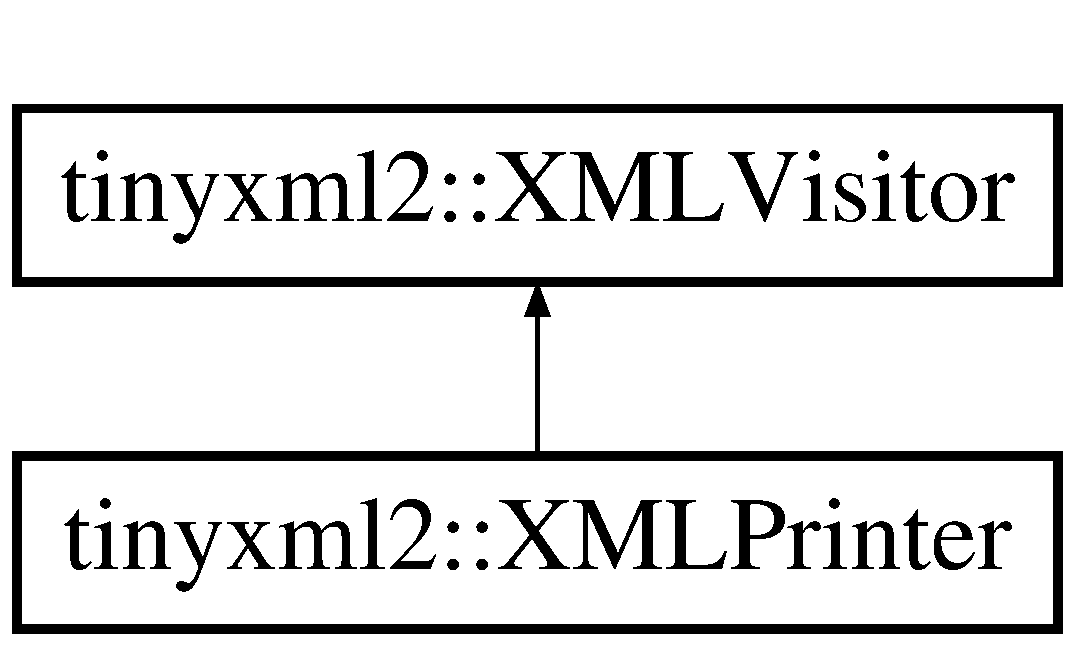
\includegraphics[height=2.000000cm]{classtinyxml2_1_1_x_m_l_visitor}
\end{center}
\end{figure}
\subsection*{Public Member Functions}
\begin{DoxyCompactItemize}
\item 
virtual \mbox{\hyperlink{classtinyxml2_1_1_x_m_l_visitor_a494e72033d646c47d9c65c502ec62364}{$\sim$\+X\+M\+L\+Visitor}} ()
\item 
virtual bool \mbox{\hyperlink{classtinyxml2_1_1_x_m_l_visitor_acb3c22fc5f60eb9db98f533f2761f67d}{Visit\+Enter}} (const \mbox{\hyperlink{classtinyxml2_1_1_x_m_l_document}{X\+M\+L\+Document}} \&)
\begin{DoxyCompactList}\small\item\em Visit a document. \end{DoxyCompactList}\item 
virtual bool \mbox{\hyperlink{classtinyxml2_1_1_x_m_l_visitor_a170e9989cd046ba904f302d087e07086}{Visit\+Exit}} (const \mbox{\hyperlink{classtinyxml2_1_1_x_m_l_document}{X\+M\+L\+Document}} \&)
\begin{DoxyCompactList}\small\item\em Visit a document. \end{DoxyCompactList}\item 
virtual bool \mbox{\hyperlink{classtinyxml2_1_1_x_m_l_visitor_af97980a17dd4e37448b181f5ddfa92b5}{Visit\+Enter}} (const \mbox{\hyperlink{classtinyxml2_1_1_x_m_l_element}{X\+M\+L\+Element}} \&, const \mbox{\hyperlink{classtinyxml2_1_1_x_m_l_attribute}{X\+M\+L\+Attribute}} $\ast$)
\begin{DoxyCompactList}\small\item\em Visit an element. \end{DoxyCompactList}\item 
virtual bool \mbox{\hyperlink{classtinyxml2_1_1_x_m_l_visitor_a772f10ddc83f881956d32628faa16eb6}{Visit\+Exit}} (const \mbox{\hyperlink{classtinyxml2_1_1_x_m_l_element}{X\+M\+L\+Element}} \&)
\begin{DoxyCompactList}\small\item\em Visit an element. \end{DoxyCompactList}\item 
virtual bool \mbox{\hyperlink{classtinyxml2_1_1_x_m_l_visitor_adc75bd459fc7ba8223b50f0616767f9a}{Visit}} (const \mbox{\hyperlink{classtinyxml2_1_1_x_m_l_declaration}{X\+M\+L\+Declaration}} \&)
\begin{DoxyCompactList}\small\item\em Visit a declaration. \end{DoxyCompactList}\item 
virtual bool \mbox{\hyperlink{classtinyxml2_1_1_x_m_l_visitor_af30233565856480ea48b6fa0d6dec65b}{Visit}} (const \mbox{\hyperlink{classtinyxml2_1_1_x_m_l_text}{X\+M\+L\+Text}} \&)
\begin{DoxyCompactList}\small\item\em Visit a text node. \end{DoxyCompactList}\item 
virtual bool \mbox{\hyperlink{classtinyxml2_1_1_x_m_l_visitor_acc8147fb5a85f6c65721654e427752d7}{Visit}} (const \mbox{\hyperlink{classtinyxml2_1_1_x_m_l_comment}{X\+M\+L\+Comment}} \&)
\begin{DoxyCompactList}\small\item\em Visit a comment node. \end{DoxyCompactList}\item 
virtual bool \mbox{\hyperlink{classtinyxml2_1_1_x_m_l_visitor_a14e4748387c34bf53d24e8119bb1f292}{Visit}} (const \mbox{\hyperlink{classtinyxml2_1_1_x_m_l_unknown}{X\+M\+L\+Unknown}} \&)
\begin{DoxyCompactList}\small\item\em Visit an unknown node. \end{DoxyCompactList}\end{DoxyCompactItemize}


\subsection{Detailed Description}
Implements the interface to the \char`\"{}\+Visitor pattern\char`\"{} (see the Accept() method.) If you call the Accept() method, it requires being passed a \mbox{\hyperlink{classtinyxml2_1_1_x_m_l_visitor}{X\+M\+L\+Visitor}} class to handle callbacks. For nodes that contain other nodes (Document, Element) you will get called with a Visit\+Enter/\+Visit\+Exit pair. Nodes that are always leafs are simply called with \mbox{\hyperlink{classtinyxml2_1_1_x_m_l_visitor_adc75bd459fc7ba8223b50f0616767f9a}{Visit()}}.

If you return \textquotesingle{}true\textquotesingle{} from a Visit method, recursive parsing will continue. If you return false, {\bfseries no children of this node or its siblings} will be visited.

All flavors of Visit methods have a default implementation that returns \textquotesingle{}true\textquotesingle{} (continue visiting). You need to only override methods that are interesting to you.

Generally Accept() is called on the \mbox{\hyperlink{classtinyxml2_1_1_x_m_l_document}{X\+M\+L\+Document}}, although all nodes support visiting.

You should never change the document from a callback.

\begin{DoxySeeAlso}{See also}
\mbox{\hyperlink{classtinyxml2_1_1_x_m_l_node_a81e66df0a44c67a7af17f3b77a152785}{X\+M\+L\+Node\+::\+Accept()}} 
\end{DoxySeeAlso}


\subsection{Constructor \& Destructor Documentation}
\mbox{\Hypertarget{classtinyxml2_1_1_x_m_l_visitor_a494e72033d646c47d9c65c502ec62364}\label{classtinyxml2_1_1_x_m_l_visitor_a494e72033d646c47d9c65c502ec62364}} 
\index{tinyxml2\+::\+X\+M\+L\+Visitor@{tinyxml2\+::\+X\+M\+L\+Visitor}!````~X\+M\+L\+Visitor@{$\sim$\+X\+M\+L\+Visitor}}
\index{````~X\+M\+L\+Visitor@{$\sim$\+X\+M\+L\+Visitor}!tinyxml2\+::\+X\+M\+L\+Visitor@{tinyxml2\+::\+X\+M\+L\+Visitor}}
\subsubsection{\texorpdfstring{$\sim$\+X\+M\+L\+Visitor()}{~XMLVisitor()}}
{\footnotesize\ttfamily virtual tinyxml2\+::\+X\+M\+L\+Visitor\+::$\sim$\+X\+M\+L\+Visitor (\begin{DoxyParamCaption}{ }\end{DoxyParamCaption})\hspace{0.3cm}{\ttfamily [inline]}, {\ttfamily [virtual]}}



\subsection{Member Function Documentation}
\mbox{\Hypertarget{classtinyxml2_1_1_x_m_l_visitor_adc75bd459fc7ba8223b50f0616767f9a}\label{classtinyxml2_1_1_x_m_l_visitor_adc75bd459fc7ba8223b50f0616767f9a}} 
\index{tinyxml2\+::\+X\+M\+L\+Visitor@{tinyxml2\+::\+X\+M\+L\+Visitor}!Visit@{Visit}}
\index{Visit@{Visit}!tinyxml2\+::\+X\+M\+L\+Visitor@{tinyxml2\+::\+X\+M\+L\+Visitor}}
\subsubsection{\texorpdfstring{Visit()}{Visit()}\hspace{0.1cm}{\footnotesize\ttfamily [1/4]}}
{\footnotesize\ttfamily virtual bool tinyxml2\+::\+X\+M\+L\+Visitor\+::\+Visit (\begin{DoxyParamCaption}\item[{const \mbox{\hyperlink{classtinyxml2_1_1_x_m_l_declaration}{X\+M\+L\+Declaration}} \&}]{ }\end{DoxyParamCaption})\hspace{0.3cm}{\ttfamily [inline]}, {\ttfamily [virtual]}}



Visit a declaration. 



Reimplemented in \mbox{\hyperlink{classtinyxml2_1_1_x_m_l_printer_acfc625b2549304b9c7eb85ebd5c5eb39}{tinyxml2\+::\+X\+M\+L\+Printer}}.

\mbox{\Hypertarget{classtinyxml2_1_1_x_m_l_visitor_af30233565856480ea48b6fa0d6dec65b}\label{classtinyxml2_1_1_x_m_l_visitor_af30233565856480ea48b6fa0d6dec65b}} 
\index{tinyxml2\+::\+X\+M\+L\+Visitor@{tinyxml2\+::\+X\+M\+L\+Visitor}!Visit@{Visit}}
\index{Visit@{Visit}!tinyxml2\+::\+X\+M\+L\+Visitor@{tinyxml2\+::\+X\+M\+L\+Visitor}}
\subsubsection{\texorpdfstring{Visit()}{Visit()}\hspace{0.1cm}{\footnotesize\ttfamily [2/4]}}
{\footnotesize\ttfamily virtual bool tinyxml2\+::\+X\+M\+L\+Visitor\+::\+Visit (\begin{DoxyParamCaption}\item[{const \mbox{\hyperlink{classtinyxml2_1_1_x_m_l_text}{X\+M\+L\+Text}} \&}]{ }\end{DoxyParamCaption})\hspace{0.3cm}{\ttfamily [inline]}, {\ttfamily [virtual]}}



Visit a text node. 



Reimplemented in \mbox{\hyperlink{classtinyxml2_1_1_x_m_l_printer_adc0e42b4f6fcb90a95630c79575d030b}{tinyxml2\+::\+X\+M\+L\+Printer}}.

\mbox{\Hypertarget{classtinyxml2_1_1_x_m_l_visitor_acc8147fb5a85f6c65721654e427752d7}\label{classtinyxml2_1_1_x_m_l_visitor_acc8147fb5a85f6c65721654e427752d7}} 
\index{tinyxml2\+::\+X\+M\+L\+Visitor@{tinyxml2\+::\+X\+M\+L\+Visitor}!Visit@{Visit}}
\index{Visit@{Visit}!tinyxml2\+::\+X\+M\+L\+Visitor@{tinyxml2\+::\+X\+M\+L\+Visitor}}
\subsubsection{\texorpdfstring{Visit()}{Visit()}\hspace{0.1cm}{\footnotesize\ttfamily [3/4]}}
{\footnotesize\ttfamily virtual bool tinyxml2\+::\+X\+M\+L\+Visitor\+::\+Visit (\begin{DoxyParamCaption}\item[{const \mbox{\hyperlink{classtinyxml2_1_1_x_m_l_comment}{X\+M\+L\+Comment}} \&}]{ }\end{DoxyParamCaption})\hspace{0.3cm}{\ttfamily [inline]}, {\ttfamily [virtual]}}



Visit a comment node. 



Reimplemented in \mbox{\hyperlink{classtinyxml2_1_1_x_m_l_printer_aa294c5c01af0ebb9114902456e4cb53c}{tinyxml2\+::\+X\+M\+L\+Printer}}.

\mbox{\Hypertarget{classtinyxml2_1_1_x_m_l_visitor_a14e4748387c34bf53d24e8119bb1f292}\label{classtinyxml2_1_1_x_m_l_visitor_a14e4748387c34bf53d24e8119bb1f292}} 
\index{tinyxml2\+::\+X\+M\+L\+Visitor@{tinyxml2\+::\+X\+M\+L\+Visitor}!Visit@{Visit}}
\index{Visit@{Visit}!tinyxml2\+::\+X\+M\+L\+Visitor@{tinyxml2\+::\+X\+M\+L\+Visitor}}
\subsubsection{\texorpdfstring{Visit()}{Visit()}\hspace{0.1cm}{\footnotesize\ttfamily [4/4]}}
{\footnotesize\ttfamily virtual bool tinyxml2\+::\+X\+M\+L\+Visitor\+::\+Visit (\begin{DoxyParamCaption}\item[{const \mbox{\hyperlink{classtinyxml2_1_1_x_m_l_unknown}{X\+M\+L\+Unknown}} \&}]{ }\end{DoxyParamCaption})\hspace{0.3cm}{\ttfamily [inline]}, {\ttfamily [virtual]}}



Visit an unknown node. 



Reimplemented in \mbox{\hyperlink{classtinyxml2_1_1_x_m_l_printer_ab8af5455bbf9e4be2663e6642fcd7e32}{tinyxml2\+::\+X\+M\+L\+Printer}}.

\mbox{\Hypertarget{classtinyxml2_1_1_x_m_l_visitor_acb3c22fc5f60eb9db98f533f2761f67d}\label{classtinyxml2_1_1_x_m_l_visitor_acb3c22fc5f60eb9db98f533f2761f67d}} 
\index{tinyxml2\+::\+X\+M\+L\+Visitor@{tinyxml2\+::\+X\+M\+L\+Visitor}!Visit\+Enter@{Visit\+Enter}}
\index{Visit\+Enter@{Visit\+Enter}!tinyxml2\+::\+X\+M\+L\+Visitor@{tinyxml2\+::\+X\+M\+L\+Visitor}}
\subsubsection{\texorpdfstring{Visit\+Enter()}{VisitEnter()}\hspace{0.1cm}{\footnotesize\ttfamily [1/2]}}
{\footnotesize\ttfamily virtual bool tinyxml2\+::\+X\+M\+L\+Visitor\+::\+Visit\+Enter (\begin{DoxyParamCaption}\item[{const \mbox{\hyperlink{classtinyxml2_1_1_x_m_l_document}{X\+M\+L\+Document}} \&}]{ }\end{DoxyParamCaption})\hspace{0.3cm}{\ttfamily [inline]}, {\ttfamily [virtual]}}



Visit a document. 



Reimplemented in \mbox{\hyperlink{classtinyxml2_1_1_x_m_l_printer_a9aa1de11a55a07db55a90fde37d7afad}{tinyxml2\+::\+X\+M\+L\+Printer}}.

\mbox{\Hypertarget{classtinyxml2_1_1_x_m_l_visitor_af97980a17dd4e37448b181f5ddfa92b5}\label{classtinyxml2_1_1_x_m_l_visitor_af97980a17dd4e37448b181f5ddfa92b5}} 
\index{tinyxml2\+::\+X\+M\+L\+Visitor@{tinyxml2\+::\+X\+M\+L\+Visitor}!Visit\+Enter@{Visit\+Enter}}
\index{Visit\+Enter@{Visit\+Enter}!tinyxml2\+::\+X\+M\+L\+Visitor@{tinyxml2\+::\+X\+M\+L\+Visitor}}
\subsubsection{\texorpdfstring{Visit\+Enter()}{VisitEnter()}\hspace{0.1cm}{\footnotesize\ttfamily [2/2]}}
{\footnotesize\ttfamily virtual bool tinyxml2\+::\+X\+M\+L\+Visitor\+::\+Visit\+Enter (\begin{DoxyParamCaption}\item[{const \mbox{\hyperlink{classtinyxml2_1_1_x_m_l_element}{X\+M\+L\+Element}} \&}]{,  }\item[{const \mbox{\hyperlink{classtinyxml2_1_1_x_m_l_attribute}{X\+M\+L\+Attribute}} $\ast$}]{ }\end{DoxyParamCaption})\hspace{0.3cm}{\ttfamily [inline]}, {\ttfamily [virtual]}}



Visit an element. 



Reimplemented in \mbox{\hyperlink{classtinyxml2_1_1_x_m_l_printer_a169b2509d8eabb70811b2bb8cfd1f5d1}{tinyxml2\+::\+X\+M\+L\+Printer}}.

\mbox{\Hypertarget{classtinyxml2_1_1_x_m_l_visitor_a170e9989cd046ba904f302d087e07086}\label{classtinyxml2_1_1_x_m_l_visitor_a170e9989cd046ba904f302d087e07086}} 
\index{tinyxml2\+::\+X\+M\+L\+Visitor@{tinyxml2\+::\+X\+M\+L\+Visitor}!Visit\+Exit@{Visit\+Exit}}
\index{Visit\+Exit@{Visit\+Exit}!tinyxml2\+::\+X\+M\+L\+Visitor@{tinyxml2\+::\+X\+M\+L\+Visitor}}
\subsubsection{\texorpdfstring{Visit\+Exit()}{VisitExit()}\hspace{0.1cm}{\footnotesize\ttfamily [1/2]}}
{\footnotesize\ttfamily virtual bool tinyxml2\+::\+X\+M\+L\+Visitor\+::\+Visit\+Exit (\begin{DoxyParamCaption}\item[{const \mbox{\hyperlink{classtinyxml2_1_1_x_m_l_document}{X\+M\+L\+Document}} \&}]{ }\end{DoxyParamCaption})\hspace{0.3cm}{\ttfamily [inline]}, {\ttfamily [virtual]}}



Visit a document. 



Reimplemented in \mbox{\hyperlink{classtinyxml2_1_1_x_m_l_printer_a15fc1f2b922f540917dcf52808737b29}{tinyxml2\+::\+X\+M\+L\+Printer}}.

\mbox{\Hypertarget{classtinyxml2_1_1_x_m_l_visitor_a772f10ddc83f881956d32628faa16eb6}\label{classtinyxml2_1_1_x_m_l_visitor_a772f10ddc83f881956d32628faa16eb6}} 
\index{tinyxml2\+::\+X\+M\+L\+Visitor@{tinyxml2\+::\+X\+M\+L\+Visitor}!Visit\+Exit@{Visit\+Exit}}
\index{Visit\+Exit@{Visit\+Exit}!tinyxml2\+::\+X\+M\+L\+Visitor@{tinyxml2\+::\+X\+M\+L\+Visitor}}
\subsubsection{\texorpdfstring{Visit\+Exit()}{VisitExit()}\hspace{0.1cm}{\footnotesize\ttfamily [2/2]}}
{\footnotesize\ttfamily virtual bool tinyxml2\+::\+X\+M\+L\+Visitor\+::\+Visit\+Exit (\begin{DoxyParamCaption}\item[{const \mbox{\hyperlink{classtinyxml2_1_1_x_m_l_element}{X\+M\+L\+Element}} \&}]{ }\end{DoxyParamCaption})\hspace{0.3cm}{\ttfamily [inline]}, {\ttfamily [virtual]}}



Visit an element. 



Reimplemented in \mbox{\hyperlink{classtinyxml2_1_1_x_m_l_printer_a2edd48405971a88951c71c9df86a2f50}{tinyxml2\+::\+X\+M\+L\+Printer}}.



The documentation for this class was generated from the following file\+:\begin{DoxyCompactItemize}
\item 
\mbox{\hyperlink{tinyxml2_8h}{tinyxml2.\+h}}\end{DoxyCompactItemize}

%--- End generated contents ---

% Index
\backmatter
\newpage
\phantomsection
\clearemptydoublepage
\addcontentsline{toc}{chapter}{Index}
\printindex

\end{document}
